\documentclass[twoside,11pt]{report}
% ============================================================ EX-TEST
\usepackage[utf8]{vietnam}
%\usepackage{ex_test}
\usepackage[solcolor]{ex_test} % dethi, color, loigiai, solcolor, book
\renewtheorem{ex}{\color{blue!90!black} Câu}
\usepackage{amsmath,amssymb,tikz,mathrsfs,tkz-tab}
\usepackage{fontawesome}
\usepackage[many]{tcolorbox}
\usetikzlibrary{calc}
\usepackage{geometry}
\renewcommand{\baselinestretch}{1.5}
\usepackage[locale=DE]{siunitx} % cách viết số đo có đơn vị theo chuẩn DE (gần giống VN) 
\usepackage{setspace} % hỗ trợ định dạng khoảng cách văn bản.
\usepackage[newparttoc]{titlesec}	% định dạng tiêu đề cho các section
\usepackage{currfile}
\usepackage[version=3]{mhchem} % công thức và phương trình hóa học 
\usepackage{tikz} % gói TikZ vẽ hình 
\usetikzlibrary{decorations.shapes,shapes.geometric,calc,positioning}
\usepackage{pgf} % hỗ trợ phép tính toán học và vẽ hình	
\usetikzlibrary{shapes.geometric, arrows}
\usepackage{pgfplots}
\renewcommand{\baselinestretch}{1.2}
\usepackage{tabularx}
\usepackage{makecell}
\usepackage{titlesec}
\usepackage{titletoc}
\usepackage{colortbl}
\usepackage{capt-of}
\usepackage{tkz-euclide}
% lệnh siunit 
\newcommand{\xsi}[2]{\SI[parse-numbers=false]{#1}{#2}}
\newcommand{\outfooter}{
\color{purple}\bfseries	GV: Lương Hoàng Sang
}
\newcommand{\outheader}{
	\color{purple}\bfseries	Trường THCS - THPT Nguyễn Khuyến
}
\newcommand{\namhoc}{
	\color{purple}\bfseries	Năm học: 2024 - 2025
}
\def\monhoc{\color{purple}\bfseries Vật lí 10}%{\bfseries Kế hoạch bài dạy vật lí 10}
\graphicspath{{figs/}{extra/}} % các thư mục chứa hình ảnh 
% ========== PAPER FORMAT ====================
% --- paper size 
\geometry{
	a4paper	% khổ giấy A4
	,total={180mm,260mm} % kích thước văn bản A4 170mmx247mm
	,left=15mm % canh lề trái
	,top=10mm % canh lề trên
	,bottom=20mm
	,footskip=1.0cm % khoảng cách từ văn bản đến footer
}
% --- line spacing -- choose 1 in 2 choices 
\renewcommand{\baselinestretch}{1.2} 
%\onehalfspacing			% cách dòng đơn
%\doublespacing			% cách dòng đôi 
% ----- định dạng Header và footer
% --- trang văn bản thông thường  
\pagestyle{fancy} 
\fancyhf{}
\renewcommand{\headrulewidth}
{0pt} % độ dày đường kẻ ở header, chọn 0 để ko có dòng kẻ 
\newcommand*\cirpage[1] % tạo hình tròn quanh số trang 
{\tikz[baseline=(char.base)]
	{
		\node[
		shape=circle
		,draw=black
		,fill=gray!0
		,inner sep=2pt
		]
		(char)
		{#1};
	}
}
%\fancyhead[LO,RE]{
%	\small\outheader\hfill\namhoc
%}
\fancyfoot[LO,RE] % footer - lề trong 
{	
	\small \outfooter % tên tài liệu lấy từ phần khai báo đầu file 
}  
\fancyfoot[CO,CE] % footer - giữa trang 
{
	\small \cirpage{\thepage}
} 
\fancyfoot[LE] % footer - lề ngoài 
{
	\vspace*{-11pt}
	\hspace*{-1.1pt}\monhoc
}
\fancyfoot[RO] % footer - lề ngoài 
{
	\vspace*{-11pt}
	\monhoc
}
% --- trang Part và terter title 
\fancypagestyle{plain} % mặc định của trang Part và Chapter title 
{
	\fancyfoot[LO,RE]
	{
		\small \outfooter
	}
	\fancyfoot[CO,CE]
	{
		\small \cirpage{\thepage}
	} % footer - giữa trang chẵn và lẻ 
	\fancyfoot[LE]
	{
		\vspace*{-11pt}
		\hspace*{-1.1pt}\monhoc
	}
	\fancyfoot[RO]
	{
		\vspace*{-11pt}
		\monhoc
	}
} % giống với trang thường 
% ký hiệu từ font Boondox 
\DeclareFontFamily{U}{BOONDOX-cal}{\skewchar\font=45 }
\DeclareFontShape{U}{BOONDOX-cal}{m}{n}{
	<-> s*[1.05] BOONDOX-r-cal}{}
\DeclareFontShape{U}{BOONDOX-cal}{b}{n}{
	<-> s*[1.05] BOONDOX-b-cal}{}
\DeclareMathAlphabet{\bdx}{U}{BOONDOX-cal}{m}{n}
\SetMathAlphabet{\bdx}{bold}{U}{BOONDOX-cal}{b}{n}
\DeclareMathAlphabet{\bbdx}{U}{BOONDOX-cal}{b}{n}
\newcommand{\calE}{\bdx{E}}
\newcommand{\calP}{\bdx{P}}
\newcolumntype{C}[1]{>{\centering\arraybackslash}p{#1}}
\newcolumntype{M}[1]{>{\centering\arraybackslash}m{#1}}
\newcolumntype{L}[1]{>{\raggedright\arraybackslash}m{#1}}
\newcommand{\hoac}[1]{ %hệ hoặc
	\left[\begin{aligned}#1\end{aligned}\right.}
\newcommand{\heva}[1]{ %hệ và
	\left\{\begin{aligned}#1\end{aligned}\right.}

\begin{document}
	\renewcommand{\thesection}{\Roman{section}}
	\titleformat{\section}
	{\normalfont\bfseries}{PHẦN~\thesection.}{0.4em}{}
	\titlespacing{\section}{0pt}{*0}{*0.5}
	\newcolumntype{C}[1]{>{\centering\arraybackslash}p{#1}}
	\newcolumntype{M}[1]{>{\centering\arraybackslash}m{#1}}
	\newcolumntype{L}[1]{>{\raggedright\arraybackslash}p{#1}}
	\renewcommand{\theadfont}
	{
		\normalfont\bfseries
	}
	
% ====================================================== input data BT1+2
	%\setcounter{section}{0}
\section{Câu trắc nghiệm nhiều phương án lựa chọn}
\textit{Thí sinh trả lời từ câu 1 đến câu 18. Mỗi câu hỏi thí sinh chọn một phương án}
\setcounter{ex}{0}
\Opensolutionfile{ans}[ans/G12C1TN]
%-------------------------
\begin{ex}
	"Độ không tuyệt đối" là nhiệt độ ứng với
	\choice
	{\True $\SI{0}{\kelvin}$}
	{$\SI{0}{\celsius}$}
	{$\SI{273}{\celsius}$}
	{$\SI{273}{\kelvin}$}
	\loigiai{
	}
	\end{ex}
% ===================================================================
\begin{ex}
\immini{
	Hình bên mô tả chuyển động phân tử ở các thể khác nhau. Hình cầu là phân tử, mũi tên là hướng chuyển động của phân tử. Hình mô tả chuyển động phân tử tương ứng với thể rắn, thể lỏng và thể khí lần lượt là
}
{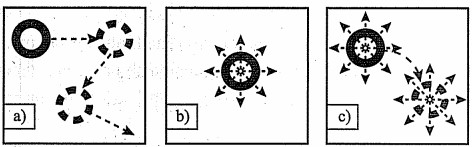
\includegraphics[scale=0.7]{figs/G12-C1-4}
}
\choice
{a), b), c)}
{\True b), c), a)}
{c), b), a)}
{b), a), c)}
	\loigiai{}
\end{ex}
% ===================================================================
\begin{ex}
	Hãy tìm ý \textbf{không đúng} với mô hình động học phân tử.
	\choice
	{Các chất được cấu tạo từ các hạt riêng biệt là phân tử}
	{Các phân tử chuyển động không ngừng}
	{\True Tốc độ chuyển động của các phân tử cấu tạo nên vật càng lớn thì thể tích của vật càng lớn}
	{Giữa các phân tử có lực tương tác gọi là lực liên kết phân tử}
	\loigiai{}
\end{ex}
% ===================================================================
\begin{ex}
	Hãy chọn phương án \textbf{sai} trong các câu sau: Cùng một khối lượng của một chất nhưng khi ở các thể tích khác nhau thì sẽ khác nhau
	\choice
	{thể tích}
	{khối lượng riêng}
	{\True kích thước của các nguyên tử}
	{trật tự của các nguyên tử}
	\loigiai{}
\end{ex}


% ===================================================================
\begin{ex}
Vật ở thể lỏng có	
	\choice
	{thể tích và hình dạng riêng, khó nén}
	{thể tích và hình dạng riêng, dễ nén}
	{\True thể tích riêng nhưng không có hình dạng riêng, khó nén}
	{thể tích riêng nhưng không có hình dạng riêng, dễ nén}
	\loigiai{}
\end{ex}

% ===================================================================
\begin{ex}
	Khi nói đến nhiệt độ của một vật ta thường nghĩ đến cảm giác "nóng" và "lạnh" của vật nhưng đó chỉ là tương đối vì cảm giác mang tính chủ quan. Cảm giác nóng, lạnh mà chúng ta cảm nhận được khi tiếp xúc với vật liên quan đến
	\choice
	{\True năng lượng nhiệt của các phân tử}
	{khối lượng của vật}
	{trọng lượng riêng của vật}
	{động năng chuyển động của vật}
	\loigiai{}
\end{ex}
% ===================================================================
\begin{ex}
	Nội năng của một vật là
	\choice
	{tổng động năng và thế năng của vật}
	{\True tổng động năng và thế năng của các phân tử cấu tạo nên vật}
	{tổng nhiệt lượng và cơ năng mà vật nhận được trong quá trình truyền nhiệt và thực hiện công}
	{nhiệt lượng vật nhận được trong quá trình truyền nhiệt}
	\loigiai{}
\end{ex}
% ===================================================================
\begin{ex}
	Phát biểu nào sau đây là \textbf{đúng}?
	\choice
	{Nội năng của một hệ nhất định phải có thế năng tương tác giữa các hạt cấu tạo nên vật}
	{Nhiệt lượng truyền cho hệ chỉ làm tăng động năng của chuyển động nhiệt của các hạt cấu tạo nên hệ}
	{\True Công mà hệ nhận được có thể làm thay đổi cả tổng động năng chuyển động nhiệt của các hạt cấu tạo nên hệ và thế năng tương tác giữa chúng}
	{Nói chung, nội năng là hàm của nhiệt độ và thể tích, nên nếu thể tích của hệ đã thay đổi thì nội năng của hệ phải thay đổi}
	\loigiai{}
\end{ex}

% ===================================================================
\begin{ex}
	Nhiệt lượng được truyền vào hỗn hợp nước đá để làm tan chảy một phần nước đá. Trong quá trình này, hỗn hợp nước đá
	\choice
	{thực hiện công}
	{có nhiệt độ tăng lên}
	{\True có nội năng tăng lên}
	{thực hiện công, có nhiệt độ tăng và nội năng cũng tăng}
	\loigiai{}
\end{ex}

% ===================================================================
\begin{ex}
	\immini{Hình bên là đồ thị phác hoạ sự thay đổi nhiệt độ theo thời gian trong quá trình chuyển thể từ rắn sang lỏng của chất rắn kết tinh và của chất rắn vô định hình tương ứng lần lượt là
	\choice
	{\True đường (3) và đường (2)}
	{đường (1) và đường (2)}
	{đường (2) và đường (3)}
	{đường (3) và đường (1)}
}{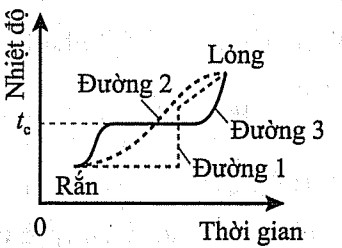
\includegraphics[scale=0.6]{figs/G12-C1-1}}
\loigiai{
\begin{itemize}
	\item Khi nung nóng liên tục một vật rắn kết tinh, nhiệt độ của vật rắn tăng dần. Khi nhiệt độ đạt đến nhiệt độ nóng chảy thì vật bắt đầu chuyển sang thể lỏng và trong suốt quá trình này nhiệt độ của vật không thay đổi. Khi toàn bộ vật rắn đã chuyển sang thể lỏng, nếu tiếp tục cung cấp nhiệt lượng thì nhiệt độ của vật sẽ tiếp tục tăng (đường 3).
	\item Khi nung nóng liên tục vật rắn vô định hình, vật rắn mềm đi và chuyển dần sang thể lỏng một cách liên tục. Trong quá trình này, nhiệt độ của vật tăng lên liên tục. Do đó, vật rắn vô định hình không có nhiệt độ nóng chảy xác định (đường 2).
\end{itemize}
}
	
\end{ex}
% ===================================================================
\begin{ex}
	Gọi $x$, $y$ và $z$ lần lượt là khoảng cách trung bình giữa các phân tử của một chất ở thể rắn, lỏng và khí. Hệ thức đúng là
	\choice
	{$z<y<x$}
	{$x<z<y$}
	{$y<x<z$}
	{\True $x<y<z$}
	\loigiai{}
\end{ex}
% ===================================================================
\begin{ex}
	Một quả bóng có khối lượng $\SI{100}{\gram}$ rơi từ độ cao $\SI{10}{\meter}$ xuống sân và nảy lên được $\SI{7}{\meter}$. Sở dĩ bóng không nảy lên được tới độ cao ban đầu là vì một phần cơ năng của quả bóng đã chuyển hoá thành nội năng của
	\choice
	{chỉ quả bóng và sân}
	{chỉ quả bóng và không khí}
	{chỉ mỗi sân và không khí}
	{\True quả bóng, mặt sân và không khí}
	\loigiai{}
\end{ex}

% ===================================================================
\begin{ex}
	Nếu thực hiện công $\SI{100}{\joule}$ để nén khí trong một xilanh thì khí truyền ra môi trường xung quanh nhiệt lượng $\SI{30}{\joule}$. Xác định độ thay đổi nội năng của khí trong cylanh.
	\choice
	{$\SI{50}{\joule}$}
	{$\SI{60}{\joule}$}
	{$\SI{30}{\joule}$}
	{\True $\SI{70}{\joule}$}
	\loigiai{Hệ nhận công và nhả nhiệt nên: $A=\SI{100}{\joule}$ và $Q=\SI{-30}{\joule}$.\\
		Độ biến thiên nội năng của khí trong xilanh:
		$$\Delta U=A+Q=\SI{70}{\joule}.$$}
\end{ex}
% ===================================================================
\begin{ex}
	Một vật được làm lạnh từ $\SI{25}{\celsius}$ xuống $\SI{5}{\celsius}$. Nhiệt độ của vật theo thang Kelvin giảm đi bao nhiêu Kelvin?
	\choice
	{$\SI{15}{\kelvin}$}
	{\True $\SI{20}{\kelvin}$}
	{$\SI{11}{\kelvin}$}
	{$\SI{18}{\kelvin}$}
	\loigiai{$$\Delta T=\Delta t=\SI{-20}{\kelvin}.$$}
\end{ex}
% ===================================================================
\begin{ex}
Một bình đựng nước ở $\SI{0.00}{\celsius}$. Người ta làm nước trong bình động đặc lại bằng cách hút không khí và hơi nước trong bình ra ngoài. Lấy nhiệt nóng chảy riêng của nước là $\SI{3.3E5}{\joule/\kilogram}$ và nhiệt hoá hơi riêng của nước là $\SI{2.48E6}{\joule/\kilogram}$. Bỏ qua sự trao đổi nhiệt với môi trường bên ngoài. Tỉ số giữa khối lượng nước bị hoá hơi và khối lượng nước ở trong bình lúc đầu là
	\choice
	{\True 0,12}
	{0,84}
	{0,16}
	{0,007}
	\loigiai{Gọi $m$ và $m'$ lần lượt là khối lượng nước ban đầu và khối lượng nước bị hoá hơi. Nhiệt lượng làm hoá hơi hoàn toàn khối lượng nước $m'$ bằng nhiệt lượng làm đông đặc hoàn toàn khối lượng nước $\left(m-m'\right)$.\\
	Ta có:
$$Q_\text{đ}=Q_h\Rightarrow \left(m-m'\right)\lambda=m'L\Rightarrow\dfrac{m'}{m}=\dfrac{\lambda}{\lambda+L}=0,12.$$}
\end{ex}
% ===================================================================
\begin{ex}
	Một học sinh, sau khi biết đến thí nghiệm nổi tiếng của Joule, đã phát triển một thiết bị đạp xe cố định (tập gym), có thể chuyển đổi toàn bộ năng lượng tiêu hao thành nhiệt để làm ấm nước. Cần bao nhiêu cơ năng để tăng nhiệt độ của $\SI{300}{\gram}$ nước $\SI{20}{\celsius}$ đến $\SI{95}{\celsius}$? Biết nhiệt dung riêng của nước là $\SI{4200}{\joule/\left(\kilogram\cdot\kelvin\right)}$.
	\choice
	{\True $\SI{94500}{\joule}$}
	{$\SI{22000}{\joule}$}
	{$\SI{5400}{\joule}$}
	{$\SI{14}{\joule}$}
	\loigiai{
$$Q=mc\Delta T=\SI{94500}{\joule}.$$
}
\end{ex}

% ===================================================================
\begin{ex}
	\immini{Một học sinh dùng một sợi dây buộc vào một vật có khối lượng $\SI{5.0E2}{\kilogram}$ đang rơi qua ròng rọc vào trục bánh guồng. Học sinh này đặt hệ thống vào một bể chứa $\SI{25.0}{\kilogram}$ nước cách nhiệt tốt. Khi vật rơi xuống sẽ làm cho bánh guồng quay và khuấy động nước. Nếu vật rơi một khoảng cách thẳng đứng $\SI{1.00E2}{\meter}$ với vận tốc không đổi thì nhiệt độ của nước tăng bao nhiêu độ? Biết nhiệt dung riêng của nước là $\SI{4.20}{\kilo\joule/\left(\kilogram\cdot\kelvin\right)}$, $g=\SI{9.81}{\meter/\second^2}$.
	\choice
	{$\SI{15}{\kelvin}$}
	{\True $\SI{4.7}{\kelvin}$}
	{$\SI{6.1}{\kelvin}$}
	{$\SI{18}{\kelvin}$}
}
{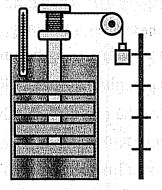
\includegraphics[scale=0.8]{figs/G12-C1-2}}
	\loigiai{Vì vật rơi với vận tốc không đổi nên độ giảm thế năng của nó dùng để làm tăng nhiệt độ cho bình nước.
	$$mgh=m'c\Delta T\Rightarrow \Delta T=\dfrac{mgh}{m'c}=\SI{4.7}{\kilogram}.$$}
\end{ex}
% ===================================================================
\begin{ex}
Một bình cách nhiệt được ngăn làm hai phần bằng một vách ngăn cách nhiệt. Hai phần bình chứa 2 chất lỏng có nhiệt dung riêng $c_1$, $c_2$ và nhiệt độ $t_1$, $t_2$ khác nhau. Bỏ vách ngăn, hai khối chất lỏng không tác dụng hoá học với nhau, nhiệt độ của chất lỏng trong bình sau khi cân bằng nhiệt là $t$. Biết rằng $t_1-t=\dfrac{1}{2}\left(t_1-t_2\right)$. Tỉ số $m_1/m_2$ là	
	\choice
	{$\dfrac{c_1}{c_2}$}
	{\True $\dfrac{c_2}{c_1}$}
	{$\sqrt{\dfrac{c_1}{c_2}}$}
	{$\sqrt{\dfrac{c_2}{c_1}}$}
	\loigiai{
Phương trình cân bằng nhiệt:
\begin{equation}
	m_1c_1\left(t_1-t\right)+m_2c_2\left(t_2-t\right)=0
	\label{eq:C1-5}
\end{equation}	
Theo đề bài, ta có:
$$t_1-t=\dfrac{1}{2}\left(t_1-t_2\right)$$
\begin{equation}
	\Rightarrow t_2-t=t-t_1
	\label{eq:C1-6}
\end{equation}
Thay (\ref{eq:C1-6}) vào (\ref{eq:C1-5}), ta được:
$$m_1c_1\left(t_1-t\right)=m_2c_2\left(t_1-t\right)\Rightarrow \dfrac{m_1}{m_2}=\dfrac{c_2}{c_1}.$$
}
\end{ex}


%-------------------------
\Closesolutionfile{ans}


\section{Câu trắc nghiệm đúng/sai} 
\textit{Thí sinh trả lời từ câu 1 đến câu 4. Trong mỗi ý \textbf{a)}, \textbf{b)}, \textbf{c)}, \textbf{d)} ở mỗi câu, thí sinh chọn đúng hoặc sai}
\setcounter{ex}{0}
\Opensolutionfile{ans}[ans/G12C1TF]
\begin{ex}
	Trong các phát biểu sau đây về sự bay hơi và sự sôi của chất lỏng, phát biểu nào đúng, phát biểu nào sai?
	\choiceTF[t]
	{\True Sự bay hơi là sự hoá hơi xảy ra ở mặt thoáng của khối chất lỏng}
	{\True Sự hoá hơi xảy ra ở cả mặt thoáng và trong lòng của khối chất lỏng khi chất lỏng sôi}
	{Sự bay hơi diễn ra chỉ ở một số nhiệt độ nhất định}
	{\True Sự sôi diễn ra ở nhiệt độ sôi}
	\loigiai{\begin{itemize}
			\item Sự hoá hơi là quá trình chuyển thể từ thể lỏng song thể khí. \item Sự hoá hơi thể hiện qua hai hình thức: sự bay hơi và sự sôi.
			\item Sự sôi xảy ra bên trong và trên bề mặt chất lỏng và chỉ xảy ra ở nhiệt độ sôi.
		\end{itemize}
	}
\end{ex}
% ===============================
\begin{ex}
Hình bên là "giản đồ chuyển thể nhiệt độ/áp suất của nước được đơn giản hoá". Trong các phát biểu sau đây, phát biểu nào đúng, phát biểu nào sai?
\begin{center}
	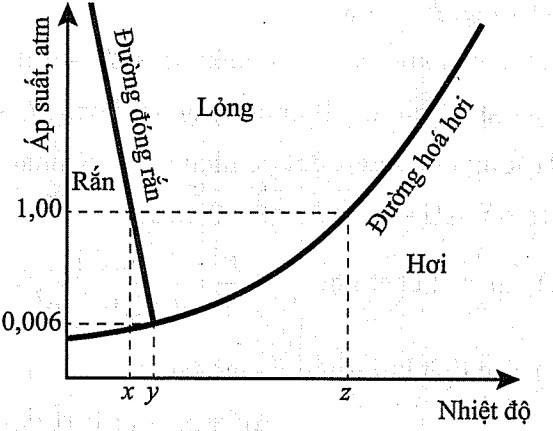
\includegraphics[scale=0.6]{figs/G12-C1-3}
\end{center}
\choiceTF[t]
{\True Thang nhiệt độ Celsius có nhiệt độ dùng làm mốc là nhiệt độ $x$ và nhiệt độ $z$}
{\True Thang nhiệt độ Kelvin có nhiệt độ dùng làm mốc là nhiệt độ thấp nhất mà các vật có thể đạt được (nhiệt độ không tuyệt đối) và nhiệt độ $y$}
{\True Ở nhiệt độ không tuyệt đối, tất cả các chất đều có động năng chuyển động nhiệt của các phân tử bằng không và thế năng của chúng là tối thiểu}
{Hiện nay, các nhà khoa học đã hạ thấp nhiệt độ đến $\SI{0}{\kelvin}$}	


	
	\loigiai{Thang nhiệt độ Celsius có nhiệt độ dùng làm mốc là nhiệt độ tan chảy của nước tinh khiết khi đóng băng và nhiệt độ sôi của nước tinh khiết ở áp suất tiêu chuẩn.\\
	Thang nhiệt độ Kelvin có nhiệt độ dùng làm mốc là nhiệt độ thấp nhất mà các vật có thể đạt được (nhiệt độ không tuyệt đối) và nhiệt độ mà nước tinh khiết có thể tồn tại đồng thời cả ba thể rắn, lỏng và hơi.\\
	Ở nhiệt độ không tuyệt đối, tất cả các chất đều có động năng chuyển động nhiệt của các phân tử bằng không và thế năng của chúng là tối thiểu.\\
	Vật lí học hiện đại chứng tỏ, các hạt không thể đứng yên, điều này có nghĩa chỉ có thể hạ nhiệt độ xuống gần giá trị $\SI{0}{\kelvin}$ nhưng không thể đạt đến giá trị này. Hiện nay, nhiệt độ thấp nhất mà các nhà khoa học có thể tạo ra là $\SI{3.8E-11}{\kelvin}$.
	}
\end{ex}
% ===============================
\begin{ex}
	Nhiệt nóng chảy riêng và nhiệt độ nóng chảy là thông tin, giúp ta có thể
	\choiceTF[t]
	{\True xác định được năng lượng cần cung cấp cho lò nung, thời gian nung}
	{\True thời điểm đổ kim loại nóng chảy vào khuôn, thời điểm lấy sản phẩm ra khỏi khuôn}
	{\True lựa chọn vật liệu chế tạo hợp kim phù hợp với từng yêu cầu sử dụng khác nhau}
	{\True tách các kim loại nguyên chất ra khỏi quặng hỗn hợp}	
	
	\loigiai{}
\end{ex}
% ===============================
\begin{ex}
Một bình đun nước nóng bằng điện có công suất $\SI{9.0}{\kilo\watt}$. Nước được làm nóng khi đi qua buồng đốt của bình. Nước chảy qua buồng đốt với lưu lượng $\SI{5.8E-2}{\kilogram/\second}$. Nhiệt độ của nước khi đi vào buồng đốt là $\SI{15}{\celsius}$. Cho nhiệt dung riêng của nước là $\SI{4200}{\joule/\left(\kilogram\cdot\kelvin\right)}$. Bỏ qua mọi hao phí.
	\choiceTF[t]
	{Nhiệt độ của nước khi ra khỏi buồng đốt là $\SI{50}{\celsius}$}
	{Nếu nhiệt độ của nước khi đi vào buồng đốt tăng gấp đôi thì nhiệt độ nước ra khỏi buồng đốt tăng gấp đôi}
	{\True Nếu công suất điện giảm 2 lần thì nhiệt độ nước ra khỏi buồng đốt là $\SI{33.5}{\celsius}$}
	{\True Để điều chỉnh nhiệt độ của nước ra khỏi buồng đốt, ta có thể thay đổi: công suất điện; lưu lượng nước; nhiệt độ nước đi vào}	

	\loigiai{\begin{itemchoice}
			\itemch Gọi $q$ là lưu lượng nước chảy vào buồng đốt và $\calP$ là công suất buồng đốt.\\
			Nhiệt độ của nước khi ra khỏi buồng đốt:
			$$qtc\left(t_2-t_1\right)=\calP t\Rightarrow t_2=t_1+\dfrac{\calP}{qc}\approx\SI{51.9}{\celsius}.$$
			\itemch Sai vì $t_2=t_1+\dfrac{\calP}{qc}$.
			\itemch Đúng. 
			$$t'_2=t_1+\dfrac{\calP}{2qc}=\SI{33.5}{\celsius}.$$
			\itemch Đúng. $t_2$ phụ thuộc vào $\calP$, $q$ và $t_1$.
			\end{itemchoice}
	}
\end{ex}
\Closesolutionfile{ans}
\section{Câu trắc nghiệm trả lời ngắn} \textit{Thí sinh trả lời từ câu 1 đến câu 6}
\setcounter{ex}{0}
\Opensolutionfile{ans}[ans/G12C1TL]
% ===============================================================
\begin{ex}
	Một người cọ xát một miếng sắt có khối lượng $\SI{0.25}{\kilogram}$ trên một sàn nhà. Sau một thời gian miếng sắt nóng thêm $\SI{12.0}{\celsius}$. Tính công mà người này đã thực hiện \textit{(theo đơn vị $\si{\joule}$, lấy phần nguyên)}. Giả sử rằng $\SI{40}{\percent}$ công đó được dùng làm nóng miếng sắt. Biết nhiệt dung riêng của sắt là $\SI{0.46}{\kilo\joule/\left(\kilogram\cdot\kelvin\right)}$.
	\shortans{$\SI{3450}{}$}
	\loigiai{
		$$0,4A=mc\Delta T\Rightarrow A=\SI{3450}{\joule}.$$
	}
\end{ex}
% ===============================================================
\begin{ex}
	Một viên đạn chì phải có tốc độ tối thiểu là bao nhiêu để khi nó va chạm vào vật cản cứng thì nóng chảy hoàn toàn \textit{(theo đơn vị $\si{\meter/\second}$, lấy phần nguyên)}? Cho rằng $\SI{80.0}{\percent}$ động năng của viên đạn chuyển thành nội năng của nó khi va chạm; Nhiệt độ của viên đạn trước khi và chạm là $\SI{127}{\celsius}$. Cho biết nhiệt dung riêng của chì là $c=\SI{0.130}{\kilo\joule/\left(\kilogram\cdot\kelvin\right)}$; nhiệt độ nóng chảy của chì là $\SI{327}{\celsius}$, nhiệt nóng chảy riêng của chì là $\lambda=\SI{25.0}{\kilo\joule/\kilogram}$.
	\shortans{357}
	\loigiai{
		$$\SI{80}{\percent}\cdot\dfrac{1}{2}mv^2=mc\Delta T+m\lambda\Rightarrow v=\sqrt{\dfrac{2\left(c\Delta T+\lambda\right)}{0,8}}\approx\SI{357}{\meter/\second}.$$
	}
	\end{ex}
	% ===============================================================
\begin{ex}
	Một vật có khối lượng $\SI{1.00}{\kilogram}$ trượt trên một mặt phẳng nghiêng dài $\SI{0.800}{\meter}$ đặt nghiêng $\SI{30.0}{\degree}$. Ở đỉnh của mặt phẳng nghiêng, vận tốc của vật bằng 0; trượt tới chân mặt phẳng nghiêng, tốc độ của vật đạt $\SI{1.10}{\meter/\second}$. Lấy $g=\SI{9.81}{\meter/\second^2}$. Tính nhiệt lượng do vật toả ra do ma sát \textit{(theo đơn vị $\si{\joule}$, lấy đến hai chữ số ở phần thập phân)}.
	\shortans{3,32}
	\loigiai{
		Nhiệt lượng tăng thêm bằng độ lớn công của lực cản và bằng độ giảm cơ năng:
		$$Q=mgh-\dfrac{1}{2}mv^2=mgL\sin\SI{30.0}{\degree}-\dfrac{1}{2}mv^2=\SI{3.32}{\joule}.$$
	}
\end{ex}
	% ===============================================================
\begin{ex}
Ở nhiệt độ $\SI{27}{\celsius}$, các phân tử oxygen chuyển động với tốc độ trung bình khoảng $\SI{500}{\meter/\second}$. Khối lượng của phân tử oxygen là $\SI{53.2E-27}{\kilogram}$. Động năng trung bình của $\SI{E21}{}$ phân tử oxygen bằng bao nhiêu \textit{(viết đáp số 3 kí tự số)}?
	\shortans{6,65}
	\loigiai{
	$$W_\text{đ}=\dfrac{1}{2}Nmv^2=\SI{6.65}{\joule}.$$
	}
\end{ex}
	% ===============================================================
\begin{ex}
Nhiệt lượng kế bằng đồng chứa nước ở $\SI{25}{\celsius}$. Khối lượng tổng cộng của nhiệt lượng kế là $\SI{475}{\gram}$. Bỏ vào nhiệt lượng kế một vật bằng đồng có nhiệt dung riêng $c_3=\SI{0.08}{cal/\left(\gram\cdot\kelvin\right)}$, khối lượng $\SI{400}{\gram}$ ở $\SI{90}{\celsius}$. Nhiệt độ sau cùng của hệ khi cân bằng nhiệt là $\SI{30}{\celsius}$. Tính khối lượng của nhiệt lượng kế theo đơn vị gram. Biết nhiệt dung riêng của nhiệt lượng kế và nước lần lượt là $c_1=\SI{0.09}{cal/\left(\gram\cdot\kelvin\right)}$; $c_2=\SI{1}{cal/\gram\cdot\kelvin}$.
	\shortans{100}
	\loigiai{
	Áp dụng phương trình cân bằng nhiệt:
	$$Q_1+Q_2+Q_3=0$$
	\begin{equation}
		\Rightarrow 0,45m_1+5m_2=1920
		\label{eq:C1-1}
	\end{equation}
Mặt khác:
\begin{equation}
	m_1+m_2=\SI{475}{\gram}
	\label{eq:C1-2}
\end{equation}
Từ (\ref{eq:C1-1}) và (\ref{eq:C1-2}), thu được: $m_1=\SI{100}{\gram}.$
	}
\end{ex}
	% ===============================================================
\begin{ex}
	Lấy $\SI{0.01}{\kilogram}$ hơi nước ở $\SI{100}{\celsius}$ cho ngưng tụ trong bình nhiệt lượng kế chứa $\SI{0.25}{\kilogram}$ nước ở $\SI{10}{\celsius}$; nhiệt độ cuối cùng là $\SI{35}{\celsius}$. Cho nhiệt dung riêng của nước là $c=\SI{4180}{\joule/\left(\kilogram\cdot\kelvin\right)}$. Nhiệt hoá hơi riêng của nước bằng bao nhiêu \textit{(tính theo đơn vị $\SI{E6}{\joule/\kilogram}$, làm tròn đến 2 chữ số thập phân)}.
	\shortans{2,34}
	\loigiai{
		Áp dụng phương trình cân bằng nhiệt:
		$$-m_\text{h}L-m_\text{h}c\left(t_\text{cb}-100\right)+m_\text{n}c\left(t_\text{cb}-t_0\right)=0\Rightarrow L\approx\SI{2.34E6}{\joule/\kilogram}.$$
	}
\end{ex}
\Closesolutionfile{ans}
\begin{center}
	\textbf{--- HẾT ---}
\end{center}
	%\newpage\setcounter{section}{0}
\begin{center}
	\textbf{\large BẢNG ĐÁP ÁN}
\end{center}
\section{}
\inputansbox{10}{ans/G12C1TN}
\section{}
\inputansbox[2]{2}{ans/G12C1TF}
\section{}
\inputansbox[3]{6}{ans/G12C1TL}
	% ====================================================== input data BT1+2
	%\tikzstyle{startstop} = [rectangle, rounded corners, minimum width=10cm, minimum height=1.5cm,text centered, draw=black, fill=green!20]
\begin{center}
	\begin{tikzpicture}
	\node (start) [startstop] {\bfseries \text{ÔN TẬP BÀI 1 VÀ BÀI 2}};
	\end{tikzpicture}
\end{center}
\setcounter{section}{0}
\section{Câu trắc nghiệm nhiều phương án lựa chọn}
%\textit{Thí sinh trả lời từ câu 1 đến câu 18. Mỗi câu hỏi thí sinh chọn một phương án}
\setcounter{ex}{0}
\Opensolutionfile{ans}[ans/G11BT1+2TN]
% ===================================================================
\begin{ex}
	Chuyển động nào sau đây \textbf{không} được gọi là dao động cơ?
	\choice
	{Chuyển động lên xuống của piston trong cylanh của động cơ}
	{Chuyển động qua lại của con lắc đồng hồ}
	{\True Chuyển động của xe ô tô trên đường}
	{Chuyển động của dây đàn khi được gảy}
	\loigiai{}
\end{ex}
% ===================================================================
\begin{ex}
	Dao động tuần hoàn là dao động có đặc điểm
	\choice
	{vật trở lại vị trí cũ sau những khoảng thời gian bằng nhau}
	{vật có hướng chuyển động như cũ sau những khoảng thời gian bằng nhau}
	{\True vật trở lại vị trí cũ theo hướng cũ sau những khoảng thời gian bằng nhau}
	{vật trở lại vị trí cũ theo hướng cũ sau những khoảng thời gian bất kì}
	\loigiai{}
\end{ex}
% ===================================================================
\begin{ex}
Trong các phương trình sau, phương trình nào biểu diễn dao động điều hoà?
	\choice
	{$x=2\tan\left(2\pi t\right)$ cm}
	{$x=3t\cos\left(5\pi t\right)$ cm}
	{$x=\cos \left(0,5\pi t^{3}\right)$ cm}
	{\True $x=\cos\left(100\pi t\right)$ cm}
	\loigiai{}
\end{ex}
% ===================================================================
\begin{ex}
	Pha ban đầu của dao động điều hoà phụ thuộc vào
	\choice
	{\True cách chọn gốc thời gian}
	{biên độ của con lắc}
	{cách kích thích dao động}
	{cấu tạo con lắc lò xo}
	\loigiai{}
\end{ex}
% ===================================================================
\begin{ex}
	Đồ thị li độ - thời gian của một dao động điều hoà sẽ có dạng
	\choice
	{\True một đường hình sin}
	{một đoạn thẳng}
	{một đường tròn}
	{một đường thẳng}
	\loigiai{}
\end{ex}
% ===================================================================
\begin{ex}
Trong dao động điều hoà, đại lượng nào sau đây \textbf{không phải} là hằng số?	
	\choice
	{\True Li độ}
	{Biên độ}
	{Pha ban đầu}
	{Tần số góc}
	\loigiai{}
\end{ex}
% ===================================================================
\begin{ex}
Khi một vật dao động điều hoà, biên độ $A$ là	
	\choice
	{độ dịch chuyển từ vị trí cân bằng đến vị trí của vật}
	{\True độ dịch chuyển cực đại của vật tính từ vị trí cân bằng}
	{độ dịch chuyển cực đại của vật tính từ vị trí biên}
	{độ dịch chuyển của vật tính từ vị trí biên}
	\loigiai{}
\end{ex}
% ===================================================================
\begin{ex}
Trong dao động điều hoà, tần số $f$ và chu kì $T$	
	\choice
	{$f=\dfrac{1}{T^2}$}
	{$f^2=\dfrac{1}{T}$}
	{$f=T$}
	{\True $f=\dfrac{1}{T}$}
	\loigiai{}
\end{ex}
% ===================================================================
\begin{ex}
	Đại lượng nào sau đây \textbf{không phải} là một trong các đại lượng đặc trưng của một dao động điều hoà?
	\choice
	{Chu kì}
	{Tần số góc}
	{\True Pha ban đầu}
	{Tần số}
	\loigiai{}
\end{ex}
% ===================================================================
\begin{ex}
	Trong dao động điều hoà, tần số góc $\omega$ và chu kì $T$ liên hệ với nhau theo công thức 
	\choice
	{$\omega =2\pi T$}
	{\True $\omega=\dfrac{2\pi}{T}$}
	{$\omega=\dfrac{T}{2\pi}$}
	{$\omega=\dfrac{\pi}{T}$}
	\loigiai{}
\end{ex}
% ===================================================================
\begin{ex}
Các đặc trưng cơ bản của dao động điều hoà là	
	\choice
	{\True biên độ và tần số}
	{tần số và pha ban đầu}
	{bước sóng và biên độ}
	{vận tốc và gia tốc}
	\loigiai{}
\end{ex}
% ===================================================================
\begin{ex}
Để biết một vật dao động điều hoà ở đâu và đi về phía nào khi bắt đầu dao động người ta dựa vào	
	\choice
	{chu kì}
	{\True pha ban đầu}
	{li độ}
	{biên độ}
	\loigiai{}
\end{ex}
% ===================================================================
\begin{ex}
	Chu kì trong dao động điều hoà là khoảng thời gian
	\choice
	{\True để vật thực hiện một dao động}
	{để vật trở lại vị trí cũ}
	{giữa hai lần liên tiếp vật đổi chiều chuyển động}
	{giữa hai lần liên tiếp vật đi qua vị trí cân bằng}
	\loigiai{}
\end{ex}
% ===================================================================
\begin{ex}
Số dao động mà vật thực hiện được trong một giây gọi là	
	\choice
	{tần số góc}
	{\True tần số}
	{chu kì}
	{pha dao động}
	\loigiai{}
\end{ex}
% ===================================================================
\begin{ex}
	Đơn vị của tần số góc là
	\choice
	{giây $\left(\si{\second}\right)$}
	{héc $\si{\hertz}$}
	{\True radian/giây $\si{\radian/\second}$}
	{radian $\left(\si{\radian}\right)$}
	\loigiai{}
\end{ex}
% ===================================================================
\begin{ex}
	Một vật dao động điều hoà với phương trình $x=\xsi{6\cos\left(\pi t-\dfrac{\pi}{6}\right)}{\centi\meter}$, pha dao động tại thời điểm $t=\SI{2}{\second}$ là
	\choice
	{\True $\xsi{\dfrac{11\pi}{6}}{\radian}$}
	{$\xsi{-\dfrac{\pi}{6}}{\radian}$}
	{$\xsi{\dfrac{13\pi}{6}}{\radian}$}
{$\xsi{2\pi}{\radian}$}
	\loigiai{}
\end{ex}
% ===================================================================
\begin{ex}
	Đồ thị li độ - thời gian của một vật dao động điều hoà được mô tả như hình vẽ. Biên độ dao động của vật là
	\begin{center}
		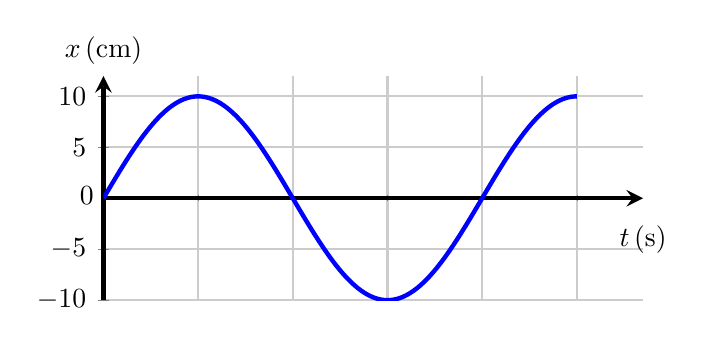
\begin{tikzpicture}  
			\begin{axis}[  ultra thick,
				xmin=0,  
				xmax=5.7, 
				ymin=-10,  
				ymax=12, 
				xtick={0,1,...,5},
				ytick={-10,-5,...,10},
				xticklabels=\empty,
%				minor x tick num=0,
%				minor y tick num=1,
				samples=300,
				axis lines=middle, 
				grid style={step=1, color=gray!20!white},
				grid=both,
				major grid style={line width=0.8pt,gray!40!white},
				xlabel=$\xsi{t}{\left(\second\right)}$, 
				ylabel=$\xsi{x}{\left(\si{\centi\meter}\right)}$, 
				every axis y label/.style={at=(current axis.above origin),anchor=south},  
				every axis x label/.style={at=(current axis.right of origin),anchor=east, below=1.5cm}, yscale=0.5 ]  
				\addplot [ultra thick, blue, smooth, domain=0:5] {10*cos(deg(pi*x/2-pi/2))}; 
			\end{axis}
		\node[label={[left]90:0}] at (0,1.2){};  
		\end{tikzpicture}
	\end{center}
	\choice
	{$\SI{20}{\centi\meter}$}
	{\True $\SI{10}{\centi\meter}$}
	{$\SI{5}{\centi\meter}$}
	{$\SI{30}{\centi\meter}$}
	\loigiai{}
\end{ex}
% ===================================================================
\begin{ex}
Một vật dao động điều hoà có đồ thị li độ - thời gian được mô tả như hình bên. Chu kì dao động của vật là	
	\begin{center}
		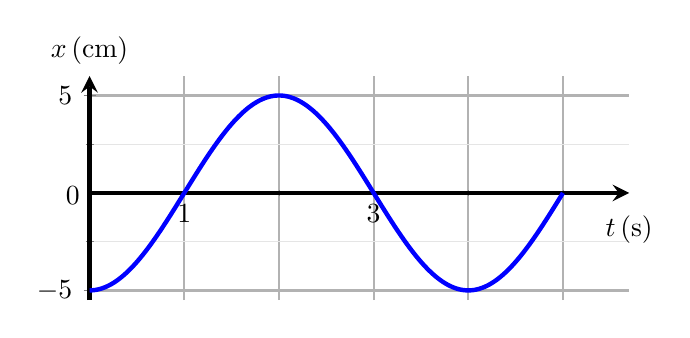
\begin{tikzpicture}  
			\begin{axis}[  ultra thick,
				xmin=0,  
				xmax=5.7, 
				ymin=-5.5,  
				ymax=6, 
				xtick={0,1,...,5},
				ytick={-5,0,5},
				xticklabels=\empty,
				%				minor x tick num=0,
							minor y tick num=1,
				samples=300,
				axis lines=middle, 
				grid style={step=1, color=gray!20!white},
				grid=both,
				major grid style={line width=0.8pt,gray!60!white},
				xlabel=$\xsi{t}{\left(\second\right)}$, 
				ylabel=$\xsi{x}{\left(\si{\centi\meter}\right)}$, 
				every axis y label/.style={at=(current axis.above origin),anchor=south},  
				every axis x label/.style={at=(current axis.right of origin),anchor=east, below=1.5cm}, yscale=0.5 ]  
				\addplot [ultra thick, blue, smooth, domain=0:5] {5*cos(deg(pi*x/2-pi))}; 
				\node at (axis cs:1,0) [below] {1};
				\node at (axis cs:3,0) [below] {3};
			\end{axis}
			\node[label={[left]90:0}] at (0,1.2){};  
		\end{tikzpicture}
	\end{center}
	\choice
	{$\SI{1}{\second}$}
	{$\SI{2}{\second}$}
	{\True $\SI{4}{\second}$}
	{$\SI{3}{\second}$}
	\loigiai{}
\end{ex}
% ===================================================================
\begin{ex}
Một vật dao động điều hoà với phương trình li độ $x=\xsi{4\cos\left(4\pi t-\dfrac{\pi}{4}\right)}{\centi\meter}$. Chu kì dao động của vật là	
	\choice
	{$\xsi{4\pi}{\second}$}
	{$\SI{2}{\second}$}
	{\True $\SI{0.5}{\second}$}
	{$\xsi{2\pi}{\second}$}
	\loigiai{}
\end{ex}
% ===================================================================
\begin{ex}
Một vật dao động điều hoà, trong thời gian 1 phút vật thực hiện được 20 dao động. Tần số dao động của vật là	
	\choice
	{\True $\xsi{\dfrac{1}{3}}{\hertz}$}
	{$\SI{3}{\hertz}$}
	{$\SI{120}{\hertz}$}
	{$\SI{20}{\hertz}$}
	\loigiai{}
\end{ex}
% ===================================================================
\begin{ex}
Cho vật dao động điều hoà có đồ thị li độ - thời gian được mô tả như hình bên. Thời gian giữa hai lần liên tiếp vật đi qua vị trí cân bằng là
	\begin{center}
		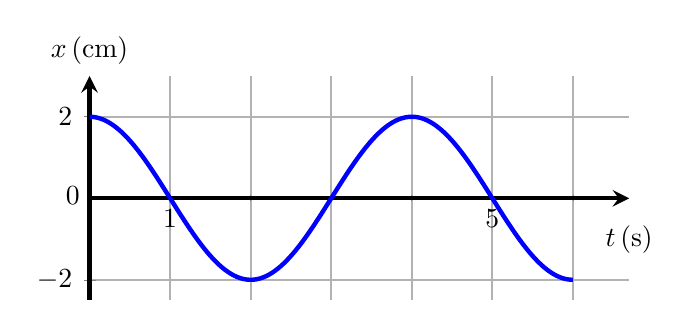
\begin{tikzpicture}  
			\begin{axis}[  ultra thick,
				xmin=0,  
				xmax=6.7, 
				ymin=-2.5,  
				ymax=3, 
				xtick={0,1,...,6},
				ytick={-2,0,2},
				xticklabels=\empty,
				%				minor x tick num=0,
				%minor y tick num=1,
				samples=300,
				axis lines=middle, 
				grid style={step=1, color=gray!20!white},
				grid=both,
				major grid style={line width=0.8pt,gray!60!white},
				xlabel=$\xsi{t}{\left(\second\right)}$, 
				ylabel=$\xsi{x}{\left(\si{\centi\meter}\right)}$, 
				every axis y label/.style={at=(current axis.above origin),anchor=south},  
				every axis x label/.style={at=(current axis.right of origin),anchor=east, below=1.5cm}, yscale=0.5 ]  
				\addplot [ultra thick, blue, smooth, domain=0:6] {2*cos(deg(pi*x/2))}; 
				\node at (axis cs:1,0) [below] {1};
				\node at (axis cs:5,0) [below] {5};
			\end{axis}
			\node[label={[left]90:0}] at (0,1.2){};  
		\end{tikzpicture}
	\end{center}
	\choice
	{$\SI{1}{\second}$}
	{$\SI{5}{\second}$}
	{$\SI{4}{\second}$}
	{\True $\SI{2}{\second}$}
	\loigiai{}
\end{ex}
% ===================================================================
\begin{ex}
	Cho hai vật dao động điều hoà với các phương trình li độ:
	$$x_1=\xsi{5\cos\left(3\pi t+\dfrac{\pi}{3}\right)}{\centi\meter}\quad \text{và}\quad x_2=\xsi{4\cos\left(3\pi t-\dfrac{\pi}{6}\right)}{\centi\meter}.$$ Độ lệch pha của hai dao động này là
	\choice
	{$\xsi{\dfrac{\pi}{3}}{\radian}$}
	{\True $\xsi{\dfrac{\pi}{2}}{\radian}$}
	{$\xsi{\dfrac{\pi}{6}}{\radian}$}
	{$\xsi{\dfrac{2\pi}{3}}{\radian}$}
	\loigiai{}
\end{ex}
% ===================================================================
\begin{ex}
Cho hai vật dao động điều hoà	cùng chu kì có đồ thị li độ - thời gian được mô tả như hình bên. Độ lệch pha giữa hai dao động là
\begin{center}
	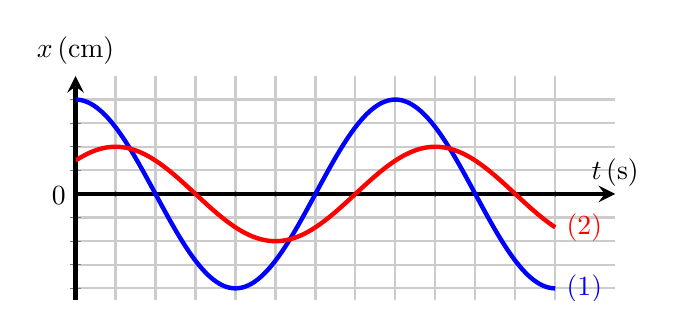
\begin{tikzpicture}  
		\begin{axis}[  ultra thick,
			xmin=0,  
			xmax=13.5, 
			ymin=-4.5,  
			ymax=5, 
			xtick={0,1,...,12},
			ytick={-4,-3,...,4},
			xticklabels=\empty,
			yticklabels=\empty,
			%				minor x tick num=0,
			%minor y tick num=1,
			samples=300,
			axis lines=middle, 
			grid style={step=1, color=gray!20!white},
			grid=both,
			major grid style={line width=0.8pt,gray!40!white},
			xlabel=$\xsi{t}{\left(\second\right)}$, 
			ylabel=$\xsi{x}{\left(\si{\centi\meter}\right)}$, 
			every axis y label/.style={at=(current axis.above origin),anchor=south},  
			every axis x label/.style={at=(current axis.right of origin),anchor=east, below=0.75cm}, yscale=0.5 ]  
			\addplot [ultra thick, blue, smooth, domain=0:12] {4*cos(deg(pi*x/4))} node [right] {(1)}; 
			\addplot [ultra thick, red, smooth, domain=0:12] {2*cos(deg(pi*x/4-pi/4))} node [right] {(2)};
		\end{axis}
		\node[label={[left]90:0}] at (0,1.2){};  
	\end{tikzpicture}
\end{center}
	\choice
	{\True $\xsi{\dfrac{\pi}{4}}{\radian}$}
	{$\xsi{\dfrac{\pi}{2}}{\radian}$}
	{$\xsi{2\pi}{\radian}$}
	{$\SI{0}{\radian}$}
	\loigiai{}
\end{ex}
% ===================================================================
\begin{ex}
Cho hai con lắc lò xo cùng dao động điều hoà có cùng tần số và cùng biên độ với phương trình li độ của con lắc thứ nhất $x_1=\xsi{4\cos\left(4\pi t+\dfrac{2\pi}{3}\right)}{\centi\meter}$. Biết thời gian con lắc thứ hai có cùng trạng thái với con lắc thứ nhất là muộn hơn $\SI{0.1}{\second}$. Phương trình dao động của con lắc thứ hai là	
	\choice
	{$x_2=\xsi{4\cos\left(4\pi t-\dfrac{\pi}{5}\right)}{\centi\meter}$}
	{$x_2=\xsi{4\cos\left(4\pi t+\dfrac{2\pi}{5}\right)}{\centi\meter}$}
	{$x_2=\xsi{4\cos\left(4\pi t-\dfrac{2\pi}{15}\right)}{\centi\meter}$}
	{$x_2=\xsi{4\cos\left(4\pi t+\dfrac{4\pi}{15}\right)}{\centi\meter}$}
	\loigiai{}
\end{ex}
% ===================================================================
\begin{ex}
	Cho hai vật dao động điều hoà cùng chu kì có đồ thị li độ - thời gian được mô tả như hình bên. Độ lệch pha giữa hai dao động là
	\begin{center}
		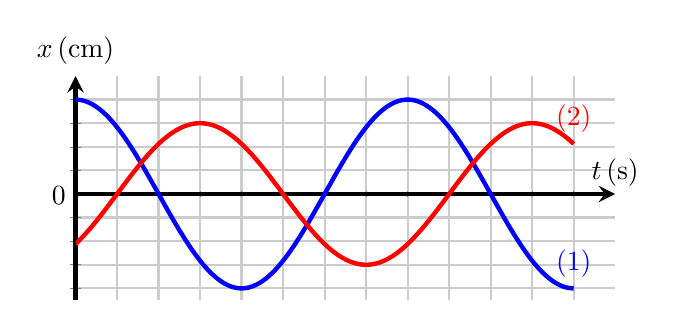
\begin{tikzpicture}  
			\begin{axis}[  ultra thick,
				xmin=0,  
				xmax=13, 
				ymin=-4.5,  
				ymax=5, 
				xtick={0,1,...,12},
				ytick={-4,-3,...,4},
				xticklabels=\empty,
				yticklabels=\empty,
				%				minor x tick num=0,
				%minor y tick num=1,
				samples=300,
				axis lines=middle, 
				grid style={step=1, color=gray!20!white},
				grid=both,
				major grid style={line width=0.8pt,gray!40!white},
				xlabel=$\xsi{t}{\left(\second\right)}$, 
				ylabel=$\xsi{x}{\left(\si{\centi\meter}\right)}$, 
				every axis y label/.style={at=(current axis.above origin),anchor=south},  
				every axis x label/.style={at=(current axis.right of origin),anchor=east, below=0.75cm}, yscale=0.5 ]  
				\addplot [ultra thick, blue, smooth, domain=0:12] {4*cos(deg(pi*x/4))} node [above] {(1)}; 
				\addplot [ultra thick, red, smooth, domain=0:12] {3*cos(deg(pi*x/4-3*pi/4))} node [above] {(2)};
			\end{axis}
			\node[label={[left]90:0}] at (0,1.2){};  
		\end{tikzpicture}
	\end{center}
	\choice
	{$\xsi{\dfrac{\pi}{4}}{\radian}$}
	{\True $\xsi{\dfrac{3\pi}{4}}{\radian}$}
	{$\xsi{2\pi}{\radian}$}
	{$\xsi{\dfrac{5\pi}{6}}{\radian}$}
	\loigiai{}
\end{ex}
\Closesolutionfile{ans}
\section{Tự luận}
\setcounter{ex}{0}
% ===================================================================
\begin{ex}
	Một vật dao động điều hoà có phương trình li độ $x=\xsi{2\cos\left(\pi t-\dfrac{\pi}{6}\right)}{\centi\meter}$, trong đó $t$ tính bằng giây. Trong $\SI{12}{\second}$ vật thực hiện được bao nhiêu dao động?
	\loigiai{$N=\dfrac{\Delta t}{T}=6$.}
\end{ex}
% ===================================================================
\begin{ex}
Xác định biên độ, chu kì, tần số và pha ban đầu của các dao động điều hoà sau:
\begin{enumerate}[label=\alph*)]
	\item $x=\xsi{5\cos\left(2\pi t-\dfrac{\pi}{2}\right)}{\centi\meter}$.
	\item $x=\xsi{-5\cos\left(\pi t-\dfrac{\pi}{6}\right)}{\centi\meter}$.
\end{enumerate}
	\loigiai{}
\end{ex}
% ===================================================================
\begin{ex}
	Một vật dao động điều hoà trên đoạn thẳng có chiều dài $\SI{4}{\centi\meter}$, vật thực hiện được 100 dao động trong $\SI{20}{\second}$. Tính biên độ, chu kì, tần số và tần số góc của dao động.
	\loigiai{}
\end{ex}
% ===================================================================
\begin{ex}
	Một vật dao động điều hoà với phương trình li độ $x=\xsi{5\cos\left(4\pi t+\dfrac{2\pi}{3}\right)}{\centi\meter}$, trong đó $t$ tính bằng giây.
	\begin{enumerate}[label=\alph*)]
		\item Xác định biên độ, tần số góc và pha ban đầu của dao động.
		\item Xác định chiều dài quỹ đạo của vật dao động.
		\item Xác định pha của dao động và li độ của vật tại các thời điểm $\SI{0.25}{\second}$ và $\SI{0.5}{\second}$.
	\end{enumerate}
	\loigiai{}
\end{ex}
% ===================================================================
\begin{ex}
	Một vật dao động điều hoà với phương trình li độ $x=\xsi{6\cos\left(3\pi t+\dfrac{\pi}{3}\right)}{\centi\meter}$ trong đó $t$ tính bằng giây. Lúc $t=\SI{2.0}{\second}$ thì các đại lượng sau đây có giá trị bằng bao nhiêu?
	\begin{enumerate}[label=\alph*)]
		\item Pha dao động.
		\item Li độ.
		\item Chu kì.
		\item Tần số.
	\end{enumerate}
	\loigiai{}
\end{ex}
% ===================================================================
\begin{ex}
	Đồ thị li độ - thời gian của hai vật dao động điều hoà $x_1\left(t\right)$ và $x_2\left(t\right)$ như hình vẽ. Xác định độ lệch pha giữa dao động của vật 1 so với dao động của vật 2.
	\begin{center}
		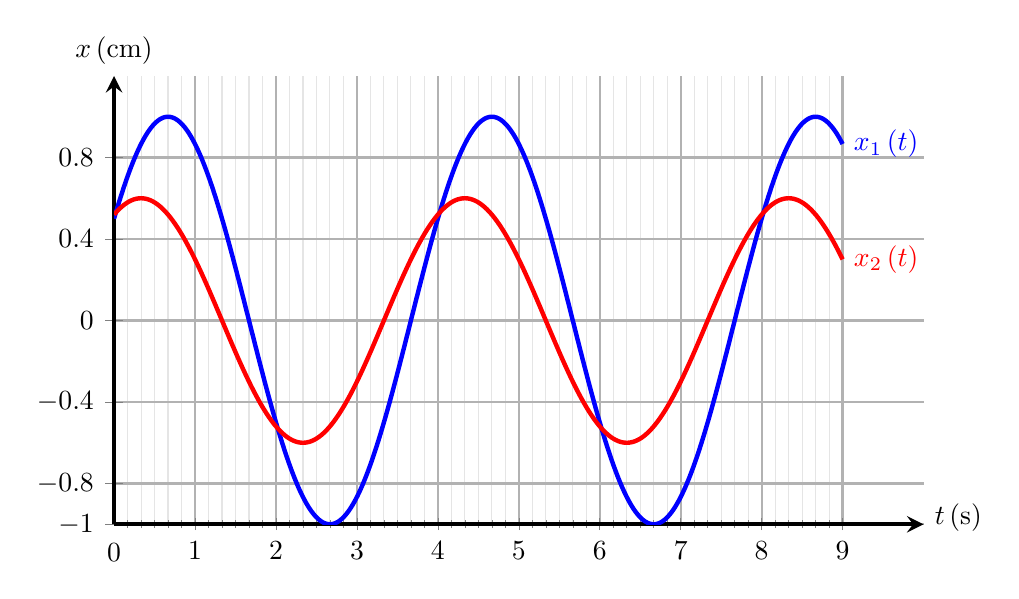
\begin{tikzpicture}  
			\begin{axis}[  ultra thick,
				xmin=0,  
				xmax=10, 
				ymin=-1,  
				ymax=1.2, 
				xtick={0,1,...,9},
				ytick={-1,-0.8,-0.4,0,0.4,0.8},
				minor x tick num=5,
				minor y tick num=1,
				samples=300,
				axis lines=middle, 
				axis x line shift={1},
				grid style={step=1, color=gray!20!white},
				grid=both,
				major grid style={line width=0.8pt,gray!60!white},
				xlabel=$\xsi{t}{\left(\second\right)}$, 
				ylabel=$\xsi{x}{\left(\si{\centi\meter}\right)}$, 
				every axis y label/.style={at=(current axis.above origin),anchor=south},  
				every axis x label/.style={at=(current axis.right of origin),below=2.5cm,anchor=west}, xscale=1.5]  
				\addplot [ultra thick, blue, smooth, domain=0:9] {1*cos(deg(pi*x/2-pi/3))} node [right] {$x_1\left(t\right)$}; 
				\addplot [ultra thick, red, smooth, domain=0:9] {0.6*cos(deg(pi*x/2-pi/6))} node [right] {$x_2\left(t\right)$};
			\end{axis}
		\node[label={[below]90:0}] at (0,-0.25){};
		\end{tikzpicture}
	\end{center}
	\loigiai{$\Delta \varphi=\xsi{\dfrac{\pi}{6}}{\radian}$.}
\end{ex}
% ===================================================================
\begin{ex}
	Đồ thị li độ - thời gian của 2 vật dao động điều hoà được thể hiện như hình vẽ.
		\begin{center}
		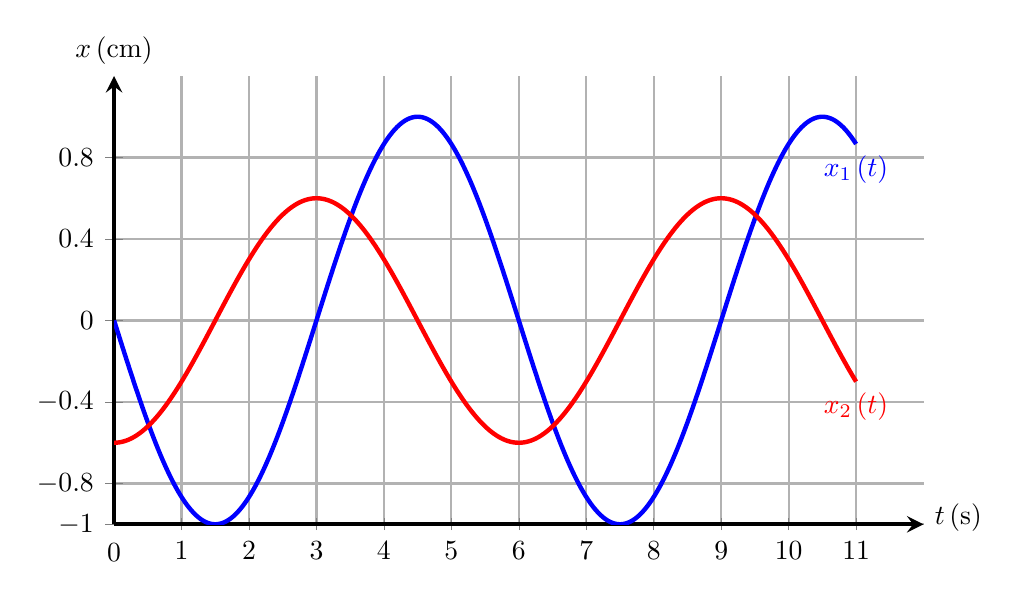
\begin{tikzpicture}  
			\begin{axis}[  ultra thick,
				xmin=0,  
				xmax=12, 
				ymin=-1,  
				ymax=1.2, 
				xtick={0,1,...,11},
				ytick={-1,-0.8,-0.4,0,0.4,0.8},
%				minor x tick num=5,
%				minor y tick num=1,
				samples=300,
				axis lines=middle, 
				axis x line shift={1},
				grid style={step=1, color=gray!20!white},
				grid=both,
				major grid style={line width=0.8pt,gray!60!white},
				xlabel=$\xsi{t}{\left(\second\right)}$, 
				ylabel=$\xsi{x}{\left(\si{\centi\meter}\right)}$, 
				every axis y label/.style={at=(current axis.above origin),anchor=south},  
				every axis x label/.style={at=(current axis.right of origin),below=2.5cm,anchor=west}, xscale=1.5]  
				\addplot [ultra thick, blue, smooth, domain=0:11] {1*cos(deg(pi*x/3+pi/2))} node [below] {$x_1\left(t\right)$}; 
				\addplot [ultra thick, red, smooth, domain=0:11] {0.6*cos(deg(pi*x/3-pi))} node [below] {$x_2\left(t\right)$};
			\end{axis}
			\node[label={[below]90:0}] at (0,-0.25){};
		\end{tikzpicture}
	\end{center}
	\begin{enumerate}[label=\alph*)]
		\item Xác định tần số của mỗi dao động.
		\item Cho biết dao động của vật 1 hay dao động của vật 2 đạt cực đại trước? Giải thích.
		\item Xác định độ lệch pha giữa dao động của vật 1 và dao động của vật 2.
	\end{enumerate}
	\loigiai{}
\end{ex}

	%\tikzstyle{startstop} = [rectangle, rounded corners, minimum width=10cm, minimum height=1.5cm,text centered, draw=black, fill=green!20]
\begin{center}
	\begin{tikzpicture}
		\node (start) [startstop] {\bfseries \text{ÔN TẬP BÀI 1 VÀ BÀI 2}};
	\end{tikzpicture}
\end{center}
\setcounter{section}{0}
\section{Câu trắc nghiệm nhiều phương án lựa chọn}
\Opensolutionfile{ans}[ans/G12BT1+2TN]
% ===================================================================
\begin{ex}
	Với mô hình động học phân tử, sự khác biệt về cấu trúc của chất rắn, chất lỏng, chất khí là do sự khác biệt về
	\choice
	{thành phần các phân tử cấu tạo của mỗi chất}
	{\True độ lớn lực tương tác giữa các phân tử trong mỗi chất}
	{số lượng phân tử cấu tạo nên mỗi chất}
	{kích thước của các phân tử cấu tạo mỗi chất}
	\loigiai{}
\end{ex}
% ===================================================================
\begin{ex}
Khi nói về khoảng cách trung bình giữa các phân tử trong chất rắn, chất lỏng, chất khí. Kết luận nào sau đây là \textbf{đúng}?	
	\choice
	{Khoảng cách giữa các phân tử trong chất lỏng xa hơn so với các phân tử trong chất khí}
	{Khoảng cách giữa các phân tử trong chất rắn xa hơn so với các phân tử trong chất lỏng}
	{\True Khoảng cách giữa các phân tử trong chất lỏng gần hơn so với các phân tử trong chất khí}
	{Khoảng cách giữa các phân tử trong chất lỏng xa hơn so với các phân tử trong chất khí}
	\loigiai{}
\end{ex}
% ===================================================================
\begin{ex}
	Câu nào dưới đây nói về đặc tính của chất rắn kết tinh là \textbf{không đúng}?
	\choice
	{Các nguyên tử, phân tử liên kết chặt với nhau và sắp xếp theo một trật tự hình học xác định}
	{\True Không có nhiệt độ nóng chảy xác định}
	{Có cấu trúc tinh thể}
	{Có nhiệt độ nóng chảy xác định}
	\loigiai{}
\end{ex}
% ===================================================================
\begin{ex}
	Chất rắn nào dưới đây thuộc loại chất rắn vô định hình?
	\choice
	{Muối ăn}
	{Nhựa đường}
	{Kim loại}
	{Kim cương}
	\loigiai{}
\end{ex}
% ===================================================================
\begin{ex}
	Chất lỏng không có hình dạng xác định vì các phân tử chất lỏng
	\choice
	{dao động tại các vị trí cân bằng xác định}
	{có thể chuyển động phân tán ra xa nhau}
	{\True dao động quanh các vị trí cân bằng có thể dịch chuyển được}
	{có thể chuyển động tự do}
	\loigiai{}
\end{ex}
% ===================================================================
\begin{ex}
Chất khí dễ bị nén hơn so với chất rắn và chất lỏng vì	
	\choice
	{lực tương tác giữa các phân tử trong chất khí lớn hơn so với lực tương tác giữa các phân tử trong chất rắn và chất lỏng}
	{\True khoảng cách giữa các phân tử trong chất khí lớn hơn so với khoảng cách giữa các phân tử trong chất rắn và chất lỏng}
	{các phân tử trong chất khí ít chuyển động hơn so với các phân tử trong chất rắn và chất lỏng}
	{các phân tử trong chất khí có kích thước nhỏ hơn so với các phân tử trong chất rắn và chất lỏng}
	\loigiai{}
\end{ex}
% ===================================================================
\begin{ex}
Khi nói về quá trình nóng chảy và đông đặc là đang nói về quá trình chuyển thể giữa	
	\choice
	{chất rắn và chất khí}
	{chất khí và chất lỏng}
	{\True chất rắn và chất lỏng}
	{các chất bất kì}
	\loigiai{}
\end{ex}
% ===================================================================
\begin{ex}
	Quá trình chuyển từ thể khí sang thể rắn của các chất được gọi là
	\choice
	{\True sự ngưng kết}
	{thăng hoa}
	{sự đông đặc}
	{sự ngưng tụ}
	\loigiai{}
\end{ex}
% ===================================================================
\begin{ex}
	Khi chất rắn kết tinh được nung nóng. Kết luận nào sau đây là \textbf{đúng}?
	\choice
	{các phân tử vẫn dao động với biên độ không đổi, khoảng cách giữa các phân tử không đổi}
	{\True các phân tử dao động với biên độ tăng lên, khoảng cách giữa các phân tử tăng lên}
	{các phân tử dao động với biên độ không đổi, khoảng cách giữa các phân tử tăng lên}
	{các phân tử dao động với biên độ tăng lên, khoảng cách giữa các phân tử không đổi}
	\loigiai{}
\end{ex}
% ===================================================================
\begin{ex}
	Sự nóng chảy của chất rắn kết tinh bắt đầu xảy ra khi
	\choice
	{một số phân tử dao động mạnh hơn các phân tử xung quanh}
	{một số phân tử va chạm với các phân tử xung quanh}
	{một số phân tử dao động mạnh lên và truyền năng lượng dao động cho các phân tử khác}
	{\True một số phân tử thắng được lực liên kết với các phân tử xung quanh và thoát khỏi liên kết với chúng}
	\loigiai{}
\end{ex}
% ===================================================================
\begin{ex}
Trong quá trình chất rắn kết tinh đang nóng chảy nhiệt độ của nó không tăng thêm là do
	\choice
	{phần nhiệt nhận thêm cân bằng với phần nhiệt toả ra môi trường bên ngoài}
	{phần nhiệt lượng nhận thêm đã chuyển thành động năng của các phân tử}
	{\True phần nhiệt lượng nhận thêm đã chuyển thành năng lượng để tiếp tục phá vỡ liên kết của mạng tinh thể}
	{phần nhiệt lượng nhận thêm đã chuyển thành thế năng của các phân tử}
	\loigiai{}
\end{ex}
% ===================================================================
\begin{ex}
	Khi cho một cục nước đá vào nước ở nhiệt độ phòng thì kết luận nào sau đây là \textbf{đúng}?
	\choice
	{Nhiệt độ của nước trong cốc từ từ tăng lên}
	{Nước trong cốc sẽ nhận nhiệt lượng từ cục nước đá}
	{\True Nhiệt lượng được truyền từ nước trong cốc cho cục nước đá}
	{Quá trình truyền nhiệt kết thúc khi cục nước đá tan hết.}
	\loigiai{}
\end{ex}
% ===================================================================
\begin{ex}
	Có ba vật A, B, C có các nhiệt độ lần lượt là $t_\text{A}$, $t_\text{B}$, $t_\text{C}$. Cho vật A tiếp xúc với vật B đến khi cân bằng nhiệt, ngay sau đó lại cho vật A tiếp xúc với vật C đến khi cân bằng nhiệt thì nhiệt độ của vật A lúc này bằng với nhiệt độ của nó lúc ban đầu khi chưa tiếp xúc với các vật khác. Kết luận nào sau đây là \textbf{đúng}?
	\choice
	{Vật B đóng vai trò truyền nhiệt lượng khi tiếp xúc với vật A}
	{Vật C đóng vai trò nhận nhiệt lượng khi tiếp xúc với vật A}
	{Nhiệt độ của vật B thấp hơn nhiệt độ của vật C}
	{\True Tổng nhiệt lượng mà vật A nhận được bằng tổng nhiệt lượng mà nó truyền cho vật khác}
	\loigiai{}
\end{ex}
% ===================================================================
\begin{ex}
	Gọi $t_1$, $t_2$ lần lượt là nhiệt độ điểm đóng băng và nhiệt độ sôi của nước tinh khiết ở điều kiện áp suất tiêu chuẩn. Trong thang nhiệt độ Celsius, mỗi độ chia $\left(\SI{1}{\celsius}\right)$ có độ lớn bằng
	\choice
	{$100\left(t_2-t_1\right)$}
	{$100\left(t_1-t_2\right)$}
	{\True $\dfrac{1}{100}\left(t_2-t_1\right)$}
	{$\dfrac{1}{273,15}\left(t_2-t_1\right)$}
	\loigiai{}
\end{ex}
% ===================================================================
\begin{ex}
Nhiệt độ không tuyệt đối là nhiệt độ mà tại đó tất cả các chất có	
	\choice
	{động năng chuyển động nhiệt của các nguyên tử hoặc phân tử bằng không và thế năng của chúng là cực đại}
	{động năng chuyển động nhiệt của các nguyên tử hoặc phân tử là cực đại và thế năng của chúng là tối thiểu}
	{\True động năng chuyển động nhiệt của các nguyên tử hoặc phân tử bằng không và thế năng của chúng là tối thiểu}
	{động năng chuyển động nhiệt của các nguyên tử hoặc phân tử và thế năng của chúng là cực đại}
	\loigiai{}
\end{ex}
% ===================================================================
\begin{ex}
Gọi $\Delta t$ và $\Delta T$ lần lượt  là độ lớn một độ chia trên thang đo nhiệt độ Celsius và thang đo nhiệt độ Kelvin. Hệ thức nào sau đây là \textbf{đúng}?
	\choice
	{$\Delta t=\dfrac{1}{273}\Delta T$}
	{$\Delta t=273\Delta T$}
	{$\Delta T=\dfrac{1}{100}\Delta t$}
	{\True $\Delta T =\Delta t$}
	\loigiai{}
\end{ex}
% ===================================================================
\begin{ex}
Kết luận nào sau đây về nhiệt độ của một vật là \textbf{đúng}?	
	\choice
	{Nhiệt độ của một vật bất kì luôn có giá trị lớn hơn $\SI{0}{\celsius}$}
	{Nhiệt độ của một vật bất kì tỉ lệ thuận với khối lượng của nó}
	{Nhiệt độ của một vật bất kì phụ thuộc vào khoảng cách giữa các phân tử trong mạng tinh thể}
	{\True Nhiệt độ của một vật bất kì không thể nhỏ hơn $\SI{0}{\kelvin}$}
	\loigiai{}
\end{ex}
% ===================================================================
\begin{ex}
Một thang nhiệt độ Z có nhiệt độ đóng băng của nước là $-\SI{12}{\degree Z}$ và khoảng cách mỗi độ chia trong thang đo nhiệt độ Z có độ lớn bằng $\SI{0.8}{}$	lần khoảng cách một độ chia trong thang đo nhiệt độ Kelvin. Nhiệt độ sôi của nước trong thang nhiệt độ Z là
	\choice
	{\True $\SI{113}{\degree Z}$}
	{$\SI{137}{\degree Z}$}
	{$\SI{68}{\degree Z}$}
	{$\SI{92}{\degree Z}$}
	\loigiai{$\Delta t_Z=0,8\Delta T\Rightarrow \left(t_Z+12\right)=0,8\cdot 100\Rightarrow t_Z=\SI{113}{\degree Z}$.}
\end{ex}
% ===================================================================
\begin{ex}
Một thang đo nhiệt độ Y, trong đó nhiệt độ nước đá đang tan là $-\SI{25}{\degree Y}$ và nhiệt độ sôi của nước là $\SI{85}{\degree Y}$. Nhiệt độ $\SI{70}{\degree Y}$ sẽ gần đúng tương ứng với nhiệt độ trong thang nhiệt độ Kelvin là	
	\choice
	{\True $\SI{360}{\kelvin}$}
	{$\SI{377}{\kelvin}$}
	{$\SI{350}{\kelvin}$}
	{$\SI{366}{\kelvin}$}
	\loigiai{
$\dfrac{t_Y+25}{85+25}=\dfrac{T-273}{100}$.	
}
% ===================================================================
\begin{ex}
Có hai thang đo nhiệt độ X và Y liên hệ với nhau theo công thức $T_\text{X}=\dfrac{3}{4}T_\text{Y}+20$. Độ biến thiên nhiệt độ $\SI{30}{\degree X}$ trong thang nhiệt X sẽ tương ứng với một độ biến thiên trong thang nhiệt Y là	
	\choice
	{$\SI{66.6}{\degree Y}$}
	{\True $\SI{40}{\degree Y}$}
	{$\SI{60}{\degree Y}$}
	{$\SI{86.6}{\degree Y}$}
	\loigiai{}
\end{ex}
\end{ex}
\Closesolutionfile{ans}
\section{Trắc nghiệm đúng/sai}
\setcounter{ex}{0}
\Opensolutionfile{ans}[ans/G12B1+2TF]
% ===================================================================
\begin{ex}
	Khi nung nóng một chất rắn kết tinh ở áp suất tiêu chuẩn, nhiệt độ của chất rắn tăng lên đến một giá trị nào đó thì chất rắn bắt đầu chuyển sang thể lỏng. Quá trình này được gọi là quá trình nóng chảy.
	\choiceTF[t]
	{\True Nhiệt độ mà chất rắn kết tinh bắt đầu nóng chảy gọi là nhiệt độ nóng chảy}
	{\True Trong quá trình nung nóng, các phân tử của chất rắn sẽ dao động mạnh làm tăng khoảng cách giữa chúng}
	{Nhiệt độ của chất rắn kết tinh tăng liên tục trong quá trình nung nóng đến khi nó nóng chảy hoàn toàn}
	{\True Sau khi chuyển sang thể lỏng, nếu ngừng cung cấp nhiệt lượng thì chất lỏng sẽ bắt đầu quá trình đông đặc}
	\loigiai{}
\end{ex}
% ===================================================================
\begin{ex}
\immini{
Máy thuỷ lực là một thiết bị quan trọng trong ngành xây dựng, kỹ thuật ô tô, \dots. Bên trong máy thuỷ lực người ta dùng một chất lỏng (dầu thuỷ lực). Khi ta tác dụng một lực $f$ lên piston nhỏ có diện tích $s$ lực này gây ra áp suất $p=f/s$ và được truyền nguyên vẹn đến piston lớn có diện tích $S$ và gây ra lực nâng $F$.	
}
{
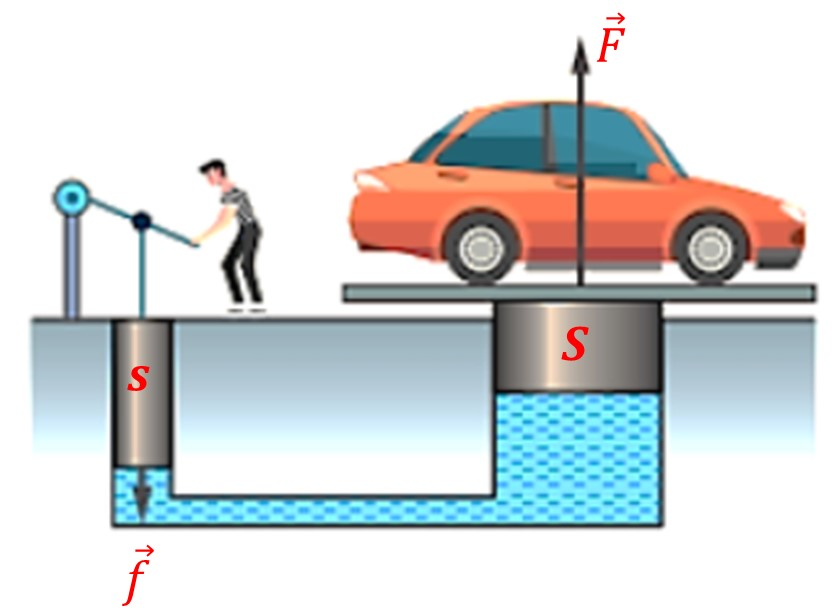
\includegraphics[width=0.6\linewidth]{figs/G12-BT1+2-1}
}
	\choiceTF[t]
	{Có thể thay thế chất lỏng trong máy thuỷ lực bằng chất khí}
	{Người ta sử dụng dầu thuỷ lực vì dầu thuỷ lực có đặc tính rất khó bị nén}
	{\True Nếu người ta nén với lực $f$ rất lón, các phân tử chất lỏng trong máy thuỷ lực càng bị nén chặt và có thể chuyển sang thể rắn}
	{Giả sử piston lớn có diện tích gấp 50 lần piston nhỏ. Khi đó, nếu muốn nâng một xe có khối lượng $\SI{1500}{\kilogram}$ thì cần tác dụng lên piston nhỏ một lực $\SI{30}{\newton}$}
	\loigiai{
\begin{itemchoice}
	\itemch Sai. Vì chất khí dễ bị nén nên máy không hoạt động được.
	\itemch Đúng.
	\itemch Sai. Chất lỏng không thể chuyển thành thể rắn khi chỉ bị nén.
	\itemch Sai. $p=\dfrac{f}{s}=\dfrac{F}{S}\Rightarrow f=\dfrac{Fs}{S}=\SI{300}{\newton}$.
	
	\end{itemchoice}	
}
\end{ex}
% ===================================================================
\begin{ex}

\immini{
Để tạo ra các loại rượu truyền thống đặc trưng của Việt Nam, các cơ sở sản xuất rượu đã thực hiện nhiều công đoạn. Trong các công đoạn đó có một công đoạn rất quan trọng là quá trình chưng cất rượu. Quá	trình chưng cất được thể hiện đơn giản bằng sơ đồ hình bên.
}
{
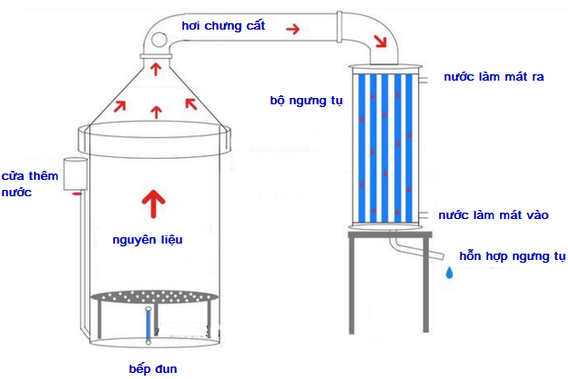
\includegraphics[width=0.7\linewidth]{figs/G12-BT1+2-2}
}
	\choiceTF[t]
	{\True Ở bồn A hỗn hợp nguyên liệu lỏng được cung cấp nhiệt lượng để tạo hơi rượu}
	{Rượu có nhiệt độ sôi cao hơn nước nên rượu hoá hơi trước}
	{Nước làm mát ở bồn B có tác dụng cung cấp nhiệt lượng cho quá trình ngưng tụ của hơi rượu}
	{\True Thực ra trong hỗn hợp hơi vừa có hơi rượu vừa có hơi nước}
	\loigiai{}
\end{ex}
% ===================================================================
\begin{ex}
	\immini{
Máy làm lạnh là một thiết bị khá quen thuộc trong đời sống hằng ngày. Nguyên tắc hoạt động của máy dựa trên nguyên tắc chuyển thể của môi chất gas bên trong máy. Sự trao đổi nhiệt với môi trường diễn ra ở giàn nóng và giàn lạnh của máy.	
}
{
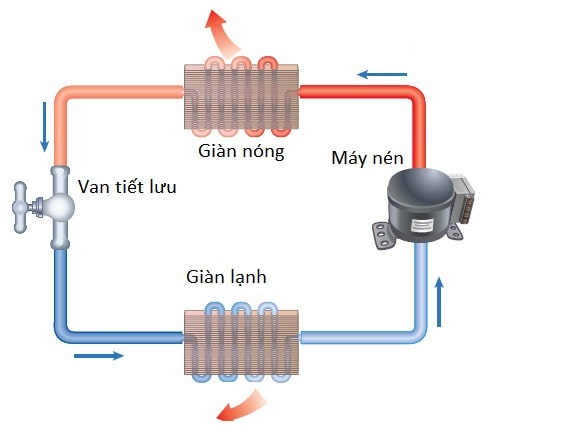
\includegraphics[width=0.65\linewidth]{figs/G12-BT1+2-3}
}
	\choiceTF[t]
	{\True Tại giàn nóng, gas có sự chuyển thể từ dạng khí sang lỏng}
	{\True Tại giàn lạnh, gas có sự chuyển thể từ dạng lỏng sang khí}
	{Tại giàn nóng, gas đã thu nhiệt từ môi trường}
	{Tại giàn lạnh, gas đã toả nhiệt ra môi trường}
	\loigiai{}
\end{ex}
% ===================================================================
\begin{ex}
	Hình bên là đồ thị phác hoạ sự thay đổi nhiệt độ theo thời gian trong quá trình chuyển thể từ rắn sang lỏng của chất rắn kết tinh và chất rắn vô định hình.
\begin{center}
	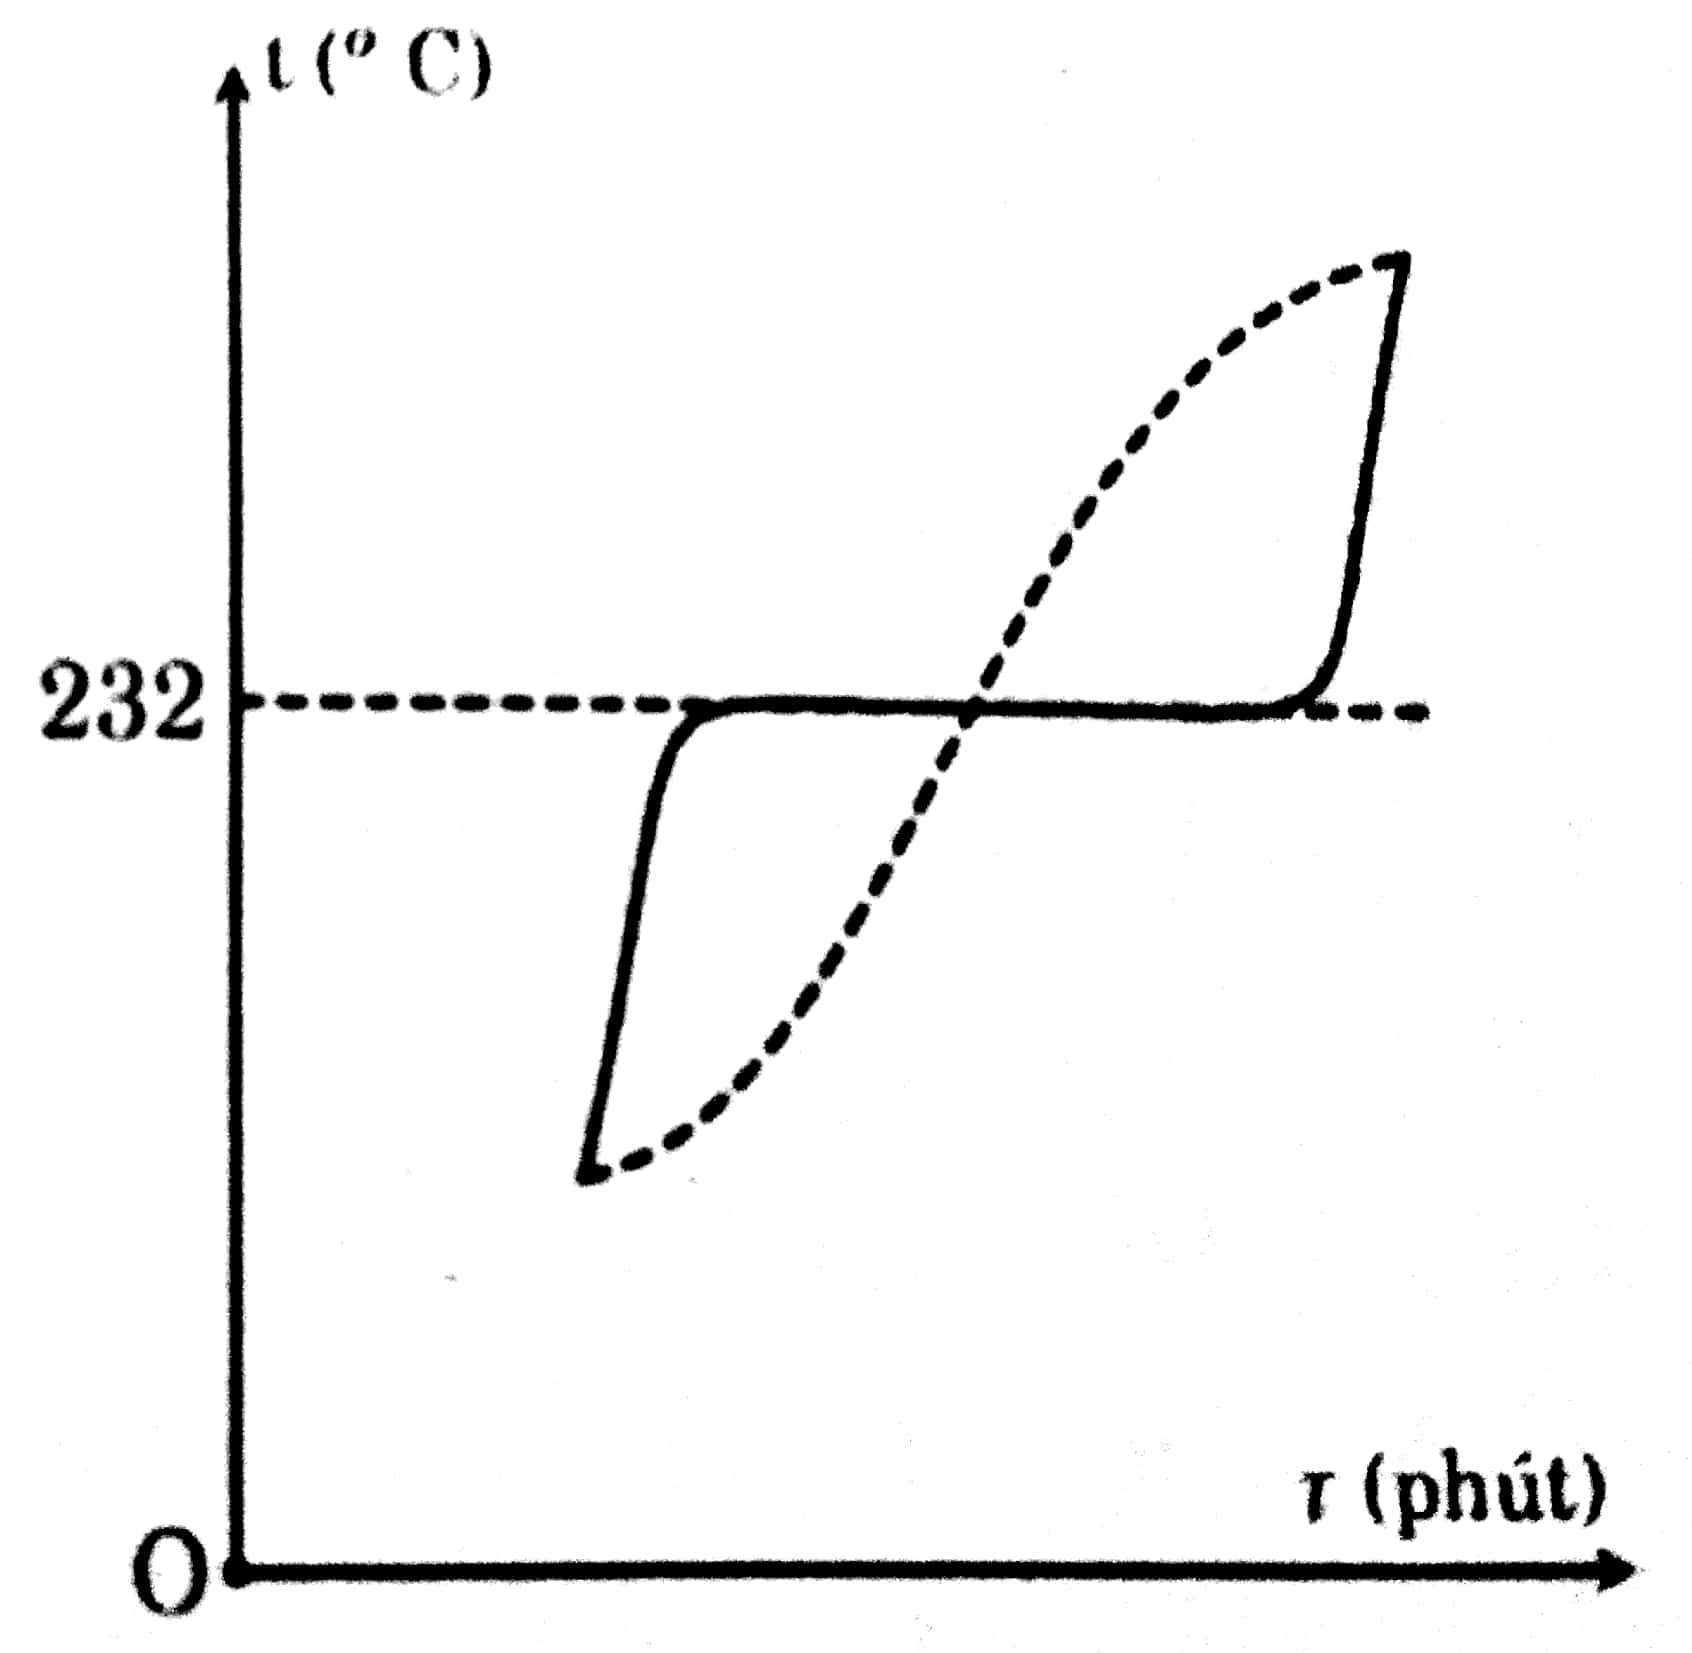
\includegraphics[width=0.3\linewidth]{figs/G12-BT1+2-4}
\end{center}
	\choiceTF[t]
	{Đường nét liền mô tả quá trình chuyển thể của chất rắn vô định hình}
	{Đường nét đứt mô tả quá trình chuyển thể của chất rắn kết tinh}
	{\True Nhiệt độ nóng chảy của chất rắn kết tinh là $\SI{232}{\celsius}$}
	{Chất rắn vô định hình có nhiệt độ nóng chảy cao hơn chất rắn kết tinh}
	\loigiai{}
\end{ex}

% ===================================================================
\begin{ex}
Có hai chai nước lạnh A và B giống nhau (cùng nhiệt độ, cùng thể tích).
\begin{enumerate}[label=\bfseries\itshape Lần \arabic*:, leftmargin=1.5cm]
	\item Nhúng chai A vào chậu nước, nhiệt độ nước trong chậu giảm xuống. Đến khi hệ cân bằng nhiệt thì lấy chai A ra khỏi chậu.
	\item Nhúng chai nước B vào chậu nước, nhiệt độ nước trong chậu tiếp tục giảm xuống đến khi cân bằng nhiệt thì lấy chai nước B ra khỏi chậu.
\end{enumerate}
	\choiceTF[t]
	{\True Nhiệt độ của chai nước A sau khi lấy ra khỏi chậu cao hơn nhiệt độ chai nước B}
	{Nhiệt lượng của chậu nước truyền cho hai chai nước là như nhau}
	{\True Độ giảm nhiệt độ của chậu nước trong lần nhúng thứ nhất nhiều hơn lần nhúng thứ hai}
	{Tổng độ tăng nhiệt độ của hai chai nước bằng tổng độ giảm nhiệt độ của chậu nước trong hai lần nhúng}
	\loigiai{}
\end{ex}
% ===================================================================
\begin{ex}
	Hình bên mô tả mối liên hệ giữa hai thang đo nhiệt độ Kelvin và Fahrenheit ở điều kiện áp suất tiêu chuẩn.
	\begin{center}
		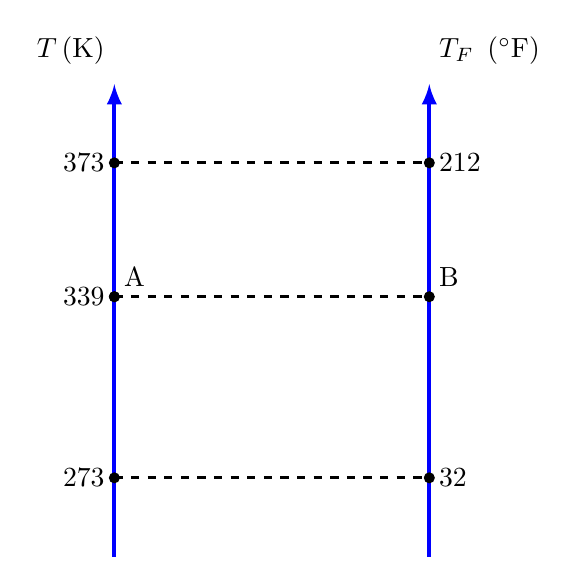
\begin{tikzpicture}
			\draw[line width=1.5pt, blue, -latex] (0,0)--(0,6);
			\draw[line width=1.5pt, blue, -latex] (4,0)--(4,6);
			\draw[line width=1pt, dashed] (0,1)--(4,1);
			\draw[line width=1pt, dashed] (0,5)--(4,5);
			\draw[line width=1pt, dashed] (0,3.3)--(4,3.3);
			\fill   (0,1) circle[radius=2pt]  node [left] {$273$};
			\fill   (4,1) circle[radius=2pt]  node [right] {$32$};
			\fill   (0,5) circle[radius=2pt]  node [left] {$373$};
			\fill   (4,5) circle[radius=2pt]  node [right] {$212$};
			\fill   (0,3.3) circle[radius=2pt]  node [left] {$339$};
			\fill   (0,3.3) circle[radius=2pt]  node [above right] {A};
			\fill   (4,3.3) circle[radius=2pt]  node [above right] {B};
			\node[label={[above left]90:$\xsi{T}{\left(\kelvin\right)}$}] at (0,6){};
			\node[label={[above right]90:$T_F\ \left(\si{\degree F}\right)$}] at (4,6){};
		\end{tikzpicture}
	\end{center}
	\choiceTF[t]
	{Mỗi độ chia trong thang đo nhiệt độ Fahrenheit có độ lớn bằng 1,8 lần mỗi độ chia trong thang đo nhiệt độ Kelvin}
	{\True Độ biến thiên nhiệt độ là $\SI{100}{\kelvin}$ trên thang đo nhiệt độ Kelvin sẽ tương ứng với độ biến thiên $\SI{180}{\degree F}$ trên thang đo nhiệt độ Fahrenheit}
	{\True Tại điểm B trên hình theo thang nhiệt độ Fahrenheit có nhiệt độ là $\SI{150.8}{\degree F}$}
	{\True Tại nhiệt độ $\SI{574.25}{}$ độ thì giá trị trên hai thang đo là bằng nhau}
	\loigiai{}
\end{ex}
% ===================================================================
\begin{ex}
Người ta dùng lò nấu chảy kim loại để nấu chảy sắt. Hình bên là đồ thị ghi lại sự thay đổi nhiệt độ của sắt theo thời gian.
\begin{center}
	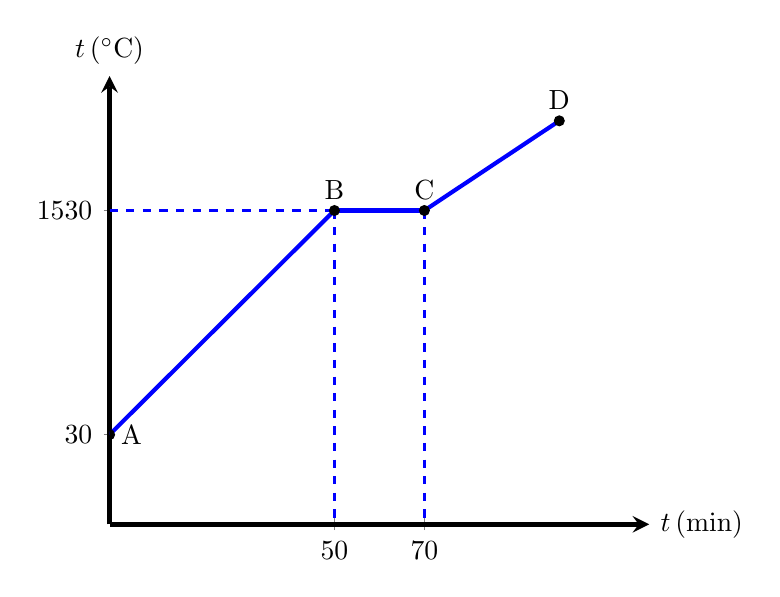
\begin{tikzpicture}  
		\begin{axis}[  ultra thick,
			xmin=0,  
			xmax=12,  
			xtick={0,5, 7},
			ytick={0,2,7},
%			minor x tick num=3,
%			minor y tick num=1,
			ymin=0,  
			ymax=10, 
			xticklabels={0,50,70},
			yticklabels={0,30,1530},
			samples=300,
			axis lines=middle, 
%			grid style={step=1,line width=0.4pt, color=gray!20!white},
%			grid=both,
%			major grid style={line width=0.8pt,gray!60!white},
			xlabel=$\xsi{t}{\left(\minute\right)}$, 
			ylabel=$\xsi{t}{\left(\si{\celsius}\right)}$, 
			every axis y label/.style={at=(current axis.above origin),anchor=south},  
			every axis x label/.style={at=(current axis.right of origin),anchor=west}]  
			\draw[line width=1.5pt, blue] (axis cs: 0,2)--(axis cs: 5,7);
			\draw[line width=1.5pt, blue] (axis cs: 5,7)--(axis cs: 7,7);
			\draw[line width=1.5pt, blue] (axis cs: 7,7)--(axis cs: 10,9);
			\draw[line width=1pt, dashed, blue] (axis cs: 5,7)--(axis cs: 5,0);
			\draw[line width=1pt, dashed, blue] (axis cs: 7,7)--(axis cs: 7,0);
			\draw[line width=1pt, dashed, blue] (axis cs: 0,7)--(axis cs: 5,7);
			\fill   (axis cs: 0,2) circle[radius=2pt]  node [right] {A};
			\fill   (axis cs: 5,7) circle[radius=2pt]  node [above] {B};
			\fill   (axis cs: 7,7) circle[radius=2pt]  node [above] {C};
			\fill   (axis cs: 10,9) circle[radius=2pt]  node [above] {D};
		\end{axis}  
	\end{tikzpicture}
\end{center}	
	\choiceTF[t]
	{\True Kể từ thời điểm ban đầu đến phút thứ 50, sắt vẫn ở thể rắn}
	{\True Nhiệt độ nóng chảy của sắt là $\SI{1530}{\celsius}$}
	{\True Từ phút thứ 50 đến phút thứ 70 là giai đoạn chuyển từ thể rắn sang thể lỏng}
	{Đoạn CD trên đồ thị thể hiện quá trình sôi của sắt}
	\loigiai{}
\end{ex}
% ===================================================================
\begin{ex}
	Giả sử có một thang đo nhiệt độ Z với nhiệt độ điểm đóng băng của nước tinh khiết là $-\SI{10}{\degree Z}$ và nhiệt độ sôi là $\SI{140}{\degree Z}$, biết rằng trong thang nhiệt độ Celsius nhiệt độ các điểm trên là $\SI{0}{\celsius}$ và $\SI{100}{\celsius}$ (các nhiệt độ đều được ghi nhận ở điều kiện áp suất tiêu chuẩn)
	\choiceTF[t]
	{\True Khoảng cách mỗi độ chia trong hai thang đo nhiệt độ là khác nhau}
	{Nếu độ biến thiên nhiệt độ là $\SI{10}{\celsius}$ trong thang nhiệt độ Celsius tương ứng với độ biến thiên $\SI{25}{\degree Z}$ trong thang nhiệt độ Z}
	{\True Nhiệt độ giữa hai thang đo nhiệt độ liên hệ với nhau $t=\dfrac{2}{3}T_\text{Z}+\dfrac{20}{3}$}
	{Nhiệt độ cơ thể người là $\SI{37}{\celsius}$ theo thang nhiệt Celsius thì tương ứng với nhiệt độ $\SI{55.5}{\degree Z}$}
	\loigiai{}
\end{ex}
\Closesolutionfile{ans}
	%\tikzstyle{startstop} = [rectangle, rounded corners, minimum width=10cm, minimum height=1.5cm,text centered, draw=black, fill=green!20]
\begin{center}
	\begin{tikzpicture}
		\node (start) [startstop] {\bfseries \text{ÔN TẬP TUẦN 4}};
	\end{tikzpicture}
\end{center}
\setcounter{section}{0}
\Opensolutionfile{ans}[ans/G10TUAN4-TN]
% ===================================================================
\begin{ex}
	Chọn đáp án có từ /cụm từ thích hợp để hoàn thành bảng sau:
	\begin{center}
		\begin{tabular}{|c|c|c|}
			\hline
			\bfseries Đơn vị &\bfseries Kí hiệu & \bfseries Đại lượng\\
			\hline
			kelvin & (1) & (2)\\
			\hline
			ampe & $\si{\ampere}$ & (3)\\
			\hline
			candela & $\si{\candela}$ & (4)\\
			\hline
		\end{tabular}
	\end{center}
	\choice
	{(1) $\si{\kelvin}$; (2) Khối lượng; (3) Cường độ dòng điện; (4) Lượng chất}
	{\True (1) $\si{\kelvin}$; (2) Nhiệt độ; (3) Cường độ dòng điện; (4) Cường độ ánh sáng}
	{(1) $\si{\kelvin}$; (2) Nhiệt độ; (3) Cường độ dòng điện; (4) Lượng chất}
	{(1) $\si{\kelvin}$; (2) Khối lượng; (3) Cường độ dòng điện; (4) Cường độ ánh sáng}
	\loigiai{}
\end{ex}
% ===================================================================
\begin{ex}
	Đơn vị nào sau đây không thuộc thứ nguyên $L$ [Chiều dài]?
	\choice
	{Dặm}
	{Hải lí}
	{Năm ánh sáng}
	{\True Năm}
	\loigiai{}
\end{ex}
% ===================================================================
\begin{ex}
Đáp án nào sau đây có 1 đơn vị cơ bản và 1 đơn vị dẫn xuất?	
	\choice
	{mét, kilogram}
	{\True newton, mol}
	{pascal, joule}
	{candela, kelvin}
	\loigiai{}
\end{ex}
% ===================================================================
\begin{ex}
	Hãy chọn câu phát biểu \textbf{đúng}?
	\choice
	{Hệ quy chiếu bao gồm hệ toạ độ, mốc thời gian và đồng hồ}
	{Hệ quy chiếu bao gồm vật làm mốc, mốc thời gian và đồng hồ}
	{Hệ quy chiếu bao gồm vật làm mốc, hệ toạ độ, mốc thời gian}
	{\True Hệ quy chiếu bao gồm vật làm mốc, hệ toạ độ, mốc thời gian và đồng hồ}
	\loigiai{}
\end{ex}
% ===================================================================
\begin{ex}
Kết luận nào sau đây là \textbf{đúng} khi nói về độ dịch chuyển và quãng đường đi được của một vật?	
	\choice
	{Độ dịch chuyển và quãng đường đi được đều là đại lượng vô hướng}
	{\True Độ dịch chuyển là đại lượng vector còn quãng đường đi được là đại lượng vô hướng}
	{Độ dịch chuyển và quãng đường đi được đều là đại lượng vector}
	{Độ dịch chuyển và quãng đường đi được đều là đại lượng không âm}
	\loigiai{}
\end{ex}
% ===================================================================
\begin{ex}
	Khi vật chuyển động thẳng đều cùng chiều dương thì đồ thị $d - t$ của vật có dạng là
	\choice
	{đường thẳng vuông góc với trục $Od$}
	{\True đường thẳng xiên góc đi lên}
	{đường thẳng xiên góc đi xuống}
	{đường thẳng vuông góc với trục $Ot$}
	\loigiai{}
\end{ex}
% ===================================================================
\begin{ex}
	Cho đồ thị độ dịch chuyển – thời gian của một vật như hình. Chọn phát biểu \textbf{đúng}.	
	\begin{center}
		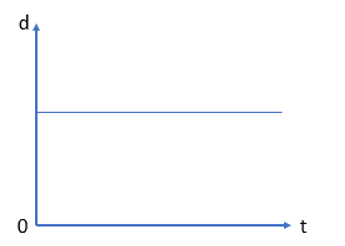
\includegraphics[width=0.25\linewidth]{figs/VN10-2023-PH-TP005-P-1}
	\end{center}
	\choice
	{Vật đang chuyển động thẳng đều theo chiều dương}
	{Vật đang chuyển động thẳng đều theo chiều âm}
	{\True Vật đang đứng yên}
	{Vật chuyển động thẳng đều theo chiều dương rồi đổi chiều chuyển động ngược lại}
	\loigiai{}
\end{ex}

% ===================================================================
\begin{ex}
Một vật bắt đầu chuyển động từ điểm O đến điểm A, sau đó chuyển động về điểm B. Quãng đường và độ dịch chuyển của vật tương ứng là	
\begin{center}
	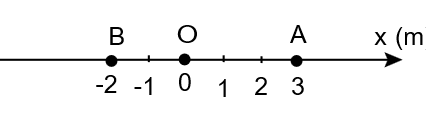
\includegraphics[width=0.4\linewidth]{figs/VN10-2022-PH-TP004-P-2}
\end{center}
	\choice
	{$\SI{2}{\meter}$; $\SI{-2}{\meter}$}
	{\True $\SI{8}{\meter}$; $\SI{-2}{\meter}$}
	{$\SI{2}{\meter}$; $\SI{2}{\meter}$}
	{$\SI{8}{\meter}$; $\SI{-8}{\meter}$}
	\loigiai{}
\end{ex}
% ===================================================================
\begin{ex}
“Lúc 15 giờ 30 phút hôm qua, xe chúng tôi đang chạy trên quốc lộ 5, cách Hải Dương 10 km”. Việc xác định vị trí của ô tô như trên còn thiếu yếu tố gì?	
	\choice
	{Vật làm mốc}
	{\True Chiều dương trên đường đi}
	{Mốc thời gian}
	{Thước đo và đồng hồ}
	\loigiai{}
\end{ex}

% ===================================================================
\begin{ex}

Hai người đi xe đạp từ A đến C, người thứ nhất đi theo đường từ A đến B, rồi từ B đến C; người thứ hai đi thẳng từ A đến C. Cả hai đều về đích cùng một lúc.\\
Hãy chọn kết luận \textbf{sai}.	
\immini{
	\choice
	{Người thứ nhất đi được quãng đường $\SI{8}{\kilo\meter}$}
	{Độ dịch chuyển của người thứ nhất và người thứ hai bằng nhau}
	{\True Độ dịch chuyển và quãng đường đi được của người thứ nhất bằng nhau}
	{Độ dịch chuyển của người thứ nhất là $\SI{5.7}{\kilo\meter}$, hướng $\SI{45}{\degree}$ Đông – Bắc}
}
	{
		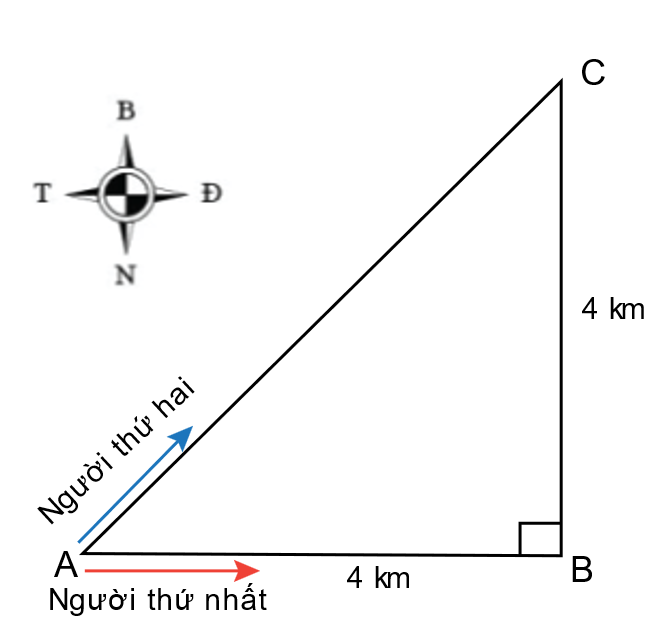
\includegraphics[width=0.5\linewidth]{figs/VN10-2022-PH-TP004-P-3}
	}
	\loigiai{}
	
\end{ex}
% ===================================================================
\begin{ex}
	Khi nhìn vào tốc kế của ô tô đang chạy, số chỉ trên tốc kế cho ta biết
	\choice
	{gia tốc tức thời của ô tô}
	{vận tốc tức thời của ô tô}
	{\True tốc độ tức thời của ô tô}
	{tốc độ trung bình của ô tô}
	\loigiai{}
\end{ex}
% ===================================================================
\begin{ex}
	Một máy bay phản lực có tốc độ $\SI{700}{\kilo\meter/\hour}$. Nếu muốn bay liên tục trên khoảng cách $\SI{1400}{\kilo\meter}$ thì máy bay phải bay trong thời gian là
	\choice
	{\True $\SI{2}{\hour}$}
	{$\SI{3}{\hour}$}
	{$\SI{2}{\hour}\SI{30}{\minute}$}
	{$\SI{1}{\hour}\SI{30}{\minute}$}
	\loigiai{Thời gian máy bay bay quãng đường $\SI{1400}{\kilo\meter}$:
		$$t=\dfrac{s}{v}=\SI{2}{\hour}.$$}
\end{ex}
% ===================================================================
\begin{ex}
	Đồ thị độ dịch chuyển – thời gian trong chuyển động thẳng của một chất điểm có dạng như hình vẽ.\\
	Trong thời gian nào xe chuyển động thẳng đều?
	\begin{center}
		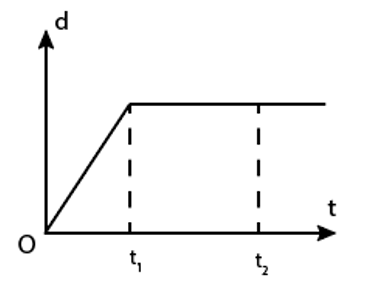
\includegraphics[width=0.25\linewidth]{figs/VN10-2023-PH-TP005-P-4}
	\end{center}
	\choice
	{\True Trong khoảng thời gian từ $0$ đến $t_1$}
	{Trong khoảng thời gian từ $0$ đến $t_2$}
	{Trong khoảng thời gian từ $t_1$ đến $t_2$}
	{Không có lúc nào xe chuyển động thẳng đều}
	\loigiai{}
\end{ex}
% ===================================================================
\begin{ex}
	Phương trình chuyển động của một chất điểm dọc theo trục $Ox$ có dạng: $x = 5 + 60t$ ($x$ đo bằng kilomét và $t$ đo bằng giờ). Chất điểm đó xuất phát từ điểm nào và chuyển động với vận tốc bằng bao nhiêu?
	\choice
	{Từ điểm $O$, với vận tốc $\SI{5}{\kilo\meter/\hour}$}
	{Từ điểm $O$, với vận tốc $\SI{60}{\kilo\meter/\hour}$}
	{Từ điểm cách $O$ $\SI{5}{\kilo\meter/\hour}$, với vận tốc $\SI{5}{\kilo\meter/\hour}$}
	{\True Từ điểm cách $O$ $\SI{5}{\kilo\meter/\hour}$, với vận tốc $\SI{60}{\kilo\meter/\hour}$}
	\loigiai{}
\end{ex}
% ===================================================================
\begin{ex}
Phương trình chuyển động của một chất điểm dọc theo $Ox$ có dạng: $x=5t-12$ (km), với $t$ đo bằng giờ. Độ dịch chuyển của chất điểm từ $\SI{2}{\hour}$ đến $\SI{4}{\hour}$ là	
	\choice
	{$\SI{8}{\kilo\meter}$}
	{$\SI{6}{\kilo\meter}$}
	{\True $\SI{10}{\kilo\meter}$}
	{$\SI{2}{\kilo\meter}$}
	\loigiai{}
\end{ex}
% ===================================================================
\begin{ex}
	Phương trình chuyển động của một chất điểm dọc theo trục $Ox$ có dạng: $x = 4 -10t$ ($x$ đo bằng kilomét và $t$ đo bằng giờ). Quãng đường đi được của chất điểm sau $\SI{2}{\hour}$ chuyển động là
	\choice
	{$\SI{-20}{\kilo\meter}$}
	{\True $\SI{20}{\kilo\meter}$}
	{$\SI{-8}{\kilo\meter}$}
	{$\SI{8}{\kilo\meter}$}
	\loigiai{}
\end{ex}

% ===================================================================
\begin{ex}
	Một xe xuất phát từ lúc 7 giờ 15 phút sáng từ thành phố M, chuyển động thẳng đều tới thành phố N, cách thành phố M $\SI{90}{\kilo\meter}$. Biết tốc độ của xe là $\SI{60}{\kilo\meter/\hour}$, xe đến thành phố N lúc
	\choice
	{9 giờ 45 phút}
	{8 giờ 30 phút}
	{9 giờ 30 phút}
	{\True 8 giờ 45 phút}
	\loigiai{Thời gian để xe đi từ M đến N:
		$$\Delta t=\dfrac{s}{v}=\SI{1.5}{\hour}.$$
		Thời điểm xe đến N:
		$$t=\SI{7}{\hour}\SI{15}{\minute}+\Delta t=\SI{8}{\hour}\SI{45}{\minute}.$$}
\end{ex}
% ===================================================================
\begin{ex}
	Trong nội dung thi đấu môn bơi ếch $\SI{100}{\meter}$, một vận động viên đã hoàn thành đường đua với thành tích $\SI{63.25}{\second}$. Tốc độ trung bình của vận động viên này trong giải thi đấu đó là bao nhiêu?
	\choice
	{\True $\SI{1.58}{\meter/\second}$}
	{$\SI{0.63}{\meter/\second}$}
	{$\SI{6.33}{\meter/\second}$}
	{$\SI{36.75}{\meter/\second}$}
	\loigiai{ Tốc độ trung bình của vận động viên này
		$$v_\text{tb}=\dfrac{s}{t}\approx\SI{1.58}{\meter/\second}.$$}
\end{ex}
% ===================================================================
\begin{ex}
Một ô tô chạy thử nghiệm trên một đoạn đường thẳng. Cứ $\SI{5}{\second}$ thì có một giọt dầu từ động cơ của ô tô rơi thẳng xuống mặt đường. Hình bên cho thấy mô hình các giọt dầu để lại trên mặt đường. Ô tô chuyển động trên đường này với tốc độ trung bình là
\begin{center}
	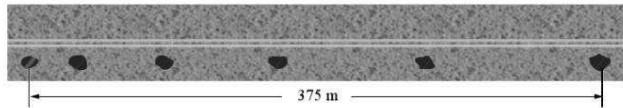
\includegraphics[width=0.5\linewidth]{figs/VN10-2022-PH-TP004-1-P-1}
\end{center}	
	\choice
	{$\SI{12.5}{\meter/\second}$}
	{\True $\SI{15}{\meter/\second}$}
	{$\SI{30}{\meter/\second}$}
	{$\SI{25}{\meter/\second}$}
	\loigiai{Tốc độ trung bình của ô tô:
		$$v_\text{tb}=\dfrac{s}{t}=\dfrac{\SI{375}{\meter}}{\SI{25}{\second}}=\SI{15}{\meter/\second}.$$}
\end{ex}
% ===================================================================
\begin{ex}
	Một xe chuyển động thẳng không đổi chiều, $\SI{1}{\hour}$ đầu xe chạy với tốc độ trung bình $\SI{60}{\kilo\meter/\hour}$ và $\SI{3}{\hour}$ sau xe chạy với tốc độ trung bình $\SI{40}{\kilo\meter/\hour}$. Tốc độ trung bình của xe trong suốt thời gian chuyển động là
	\choice
	{$\SI{48}{\kilo\meter/\hour}$}
	{$\SI{40}{\kilo\meter/\hour}$}
	{$\SI{58}{\kilo\meter/\hour}$}
	{\True $\SI{45}{\kilo\meter/\hour}$}
	\loigiai{$$v_{tb}=\dfrac{v_1t_1+v_2t_2}{t_1+t_2}=\SI{45}{\kilo\meter/\hour}.$$}
\end{ex}
% ===================================================================
\begin{ex}
	Một người đi xe đạp trên $\dfrac{2}{3}$ đoạn đường đầu với tốc độ trung bình $\SI{10}{\kilo\meter/\hour}$ và $\dfrac{1}{3}$ đoạn đường sau với tốc độ trung bình $\SI{20}{\kilo\meter/\hour}$. Tốc độ trung bình của người đi xe đạp trên cả quãng đường là
	\choice
	{\True $\SI{12}{\kilo\meter/\hour}$}
	{$\SI{15}{\kilo\meter/\hour}$}
	{$\SI{17}{\kilo\meter/\hour}$}
	{$\SI{13.3}{\kilo\meter/\hour}$}
	\loigiai{Gọi $s$ là chiều dài đoạn đường
		$$v_{tb}=\dfrac{s}{t_1+t_2}=\dfrac{s}{\dfrac{2s}{3v_1}+\dfrac{s}{3v_2}}=\dfrac{1}{\dfrac{2}{3v_1}+\dfrac{1}{3v_2}}=\SI{12}{\kilo\meter/\hour}.$$}
\end{ex}
% ===================================================================
\begin{ex}
	Hình vẽ bên là đồ thị độ dịch chuyển - thời gian của một chiếc xe ô tô chạy từ $A$ đến $B$ trên một đường thẳng. Vận tốc của xe bằng
\begin{center}
	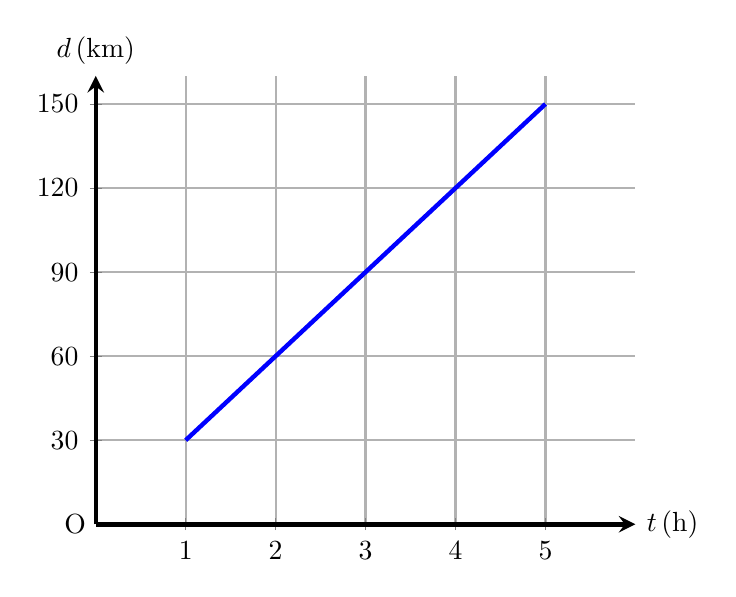
\begin{tikzpicture}  
		\begin{axis}[  ultra thick,
			xmin=0,  
			xmax=6,  
			xtick={0,1,...,5},
			ytick={0,30,...,150},
			minor x tick num=0,
			minor y tick num=0,
			ymin=0,  
			ymax=160, 
			samples=300,
			axis lines=center, 
			grid style={step=1, line width =0.4pt, color=gray!30!white},
			grid=both,
			major grid style={line width=0.8pt,gray!60!white},
			xlabel=$\xsi{t}{\left(\si{\hour}\right)}$, 		ylabel=$\xsi{d}{\left(\si{\kilo\meter}\right)}$,
			every axis y label/.style={at=(current axis.above origin),anchor=south},  
			every axis x label/.style={at=(current axis.right of origin),anchor=west},  ]
			\addplot [ultra thick, blue, smooth, domain=1:5] {30*x};			 
		\end{axis}  
		\node[left] at (0,0) {O};
	\end{tikzpicture}
\end{center}
	\choice
	{\True $\SI{30}{\kilo\meter/\hour}$}
	{$\SI{150}{\kilo\meter/\hour}$}
	{$\SI{120}{\kilo\meter/\hour}$}
	{$\SI{100}{\kilo\meter/\hour}$}
	\loigiai{}
\end{ex}
% ===================================================================
\begin{ex}
Một chất điểm chuyển động trên một đường thẳng. Đồ thị độ dịch chuyển theo thời gian của chất điểm được mô tả như hình vẽ. Tốc độ trung bình của chất điểm trong khoảng thời gian từ 0 đến $\SI{5}{\second}$ là
	\begin{center}
		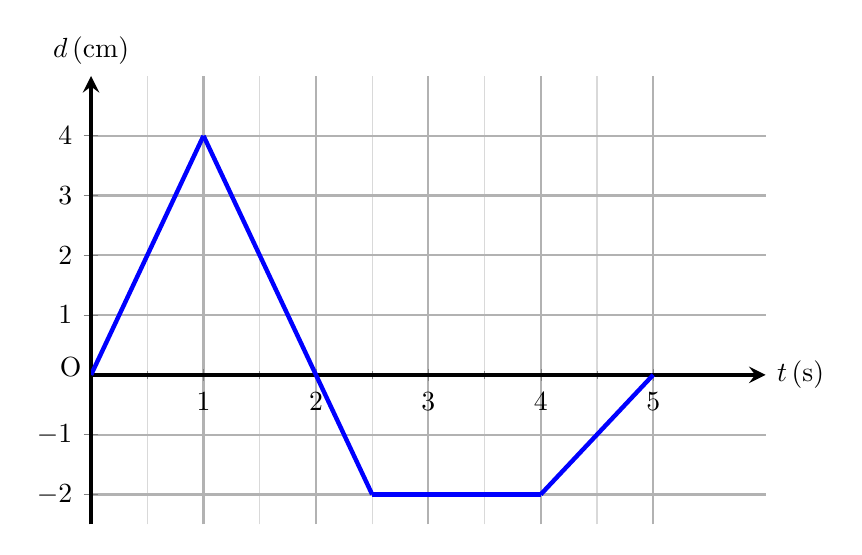
\begin{tikzpicture}  
			\begin{axis}[  ultra thick,xscale=1.25,
				xmin=0,  
				xmax=6,  
				xtick={0,1,...,5},
				ytick={-2,-1,0,1,...,4},
				minor x tick num=1,
				minor y tick num=0,
				ymin=-2.5,  
				ymax=5, 
				samples=300,
				axis lines=center, 
				grid style={step=1, line width =0.4pt, color=gray!30!white},
				grid=both,
				major grid style={line width=0.8pt,gray!60!white},
				xlabel=$\xsi{t}{\left(\si{\second}\right)}$, 		ylabel=$\xsi{d}{\left(\si{\centi\meter}\right)}$,
				every axis y label/.style={at=(current axis.above origin),anchor=south},  
				every axis x label/.style={at=(current axis.right of origin),anchor=west},  ]
				\addplot [ultra thick, blue, smooth, domain=0:1] {4*x};	
				\addplot [ultra thick, blue, smooth, domain=1:2.5] {4-4*(x-1)};		
				\addplot [ultra thick, blue, smooth, domain=2.5:4] {-2};	 
				\addplot [ultra thick, blue, smooth, domain=4:5] {-2+2*(x-4)};
				
			\end{axis}  
		\node[left] at (0,2) {O};
			
		\end{tikzpicture}
	\end{center}
	\choice
	{$\SI{1.6}{\centi\meter/\second}$}
	{$\SI{6.4}{\centi\meter/\second}$}
	{$\SI{4.8}{\centi\meter/\second}$}
	{\True $\SI{2.4}{\centi\meter/\second}$}
	\loigiai{
Tốc độ trung bình của chất điểm:
$$v_\text{tb}=\dfrac{s}{t}=\dfrac{4+4+2+2}{5}=\SI{2.4}{\centi\meter/\second}.$$	
}
\end{ex}
% ===================================================================
\begin{ex}
	Đồ thị toạ độ - thời gian của hai xe (I) và (II) cùng chuyển động trên một đường thẳng được thể hiện như hình bên. Thời điểm hai xe gặp nhau là
	\begin{center}
		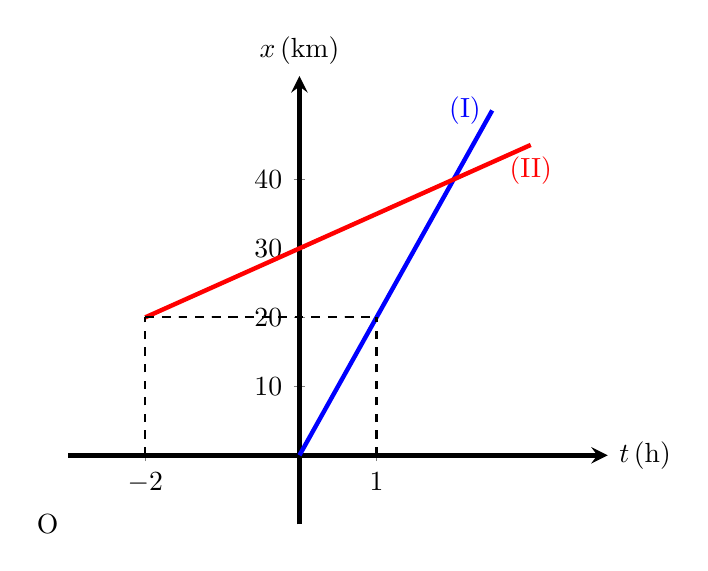
\begin{tikzpicture}  
			\begin{axis}[  ultra thick,
				xmin=-3,  
				xmax=4,  
				xtick={-2,0,1},
				ytick={0,10,...,40},
				minor x tick num=0,
				minor y tick num=0,
				ymin=-10,  
				ymax=55, 
				samples=300,
				axis lines=center, 
%				grid style={step=1, line width =0.4pt, color=gray!30!white},
%				grid=both,
%				major grid style={line width=0.8pt,gray!60!white},
				xlabel=$\xsi{t}{\left(\si{\hour}\right)}$, 		ylabel=$\xsi{x}{\left(\si{\kilo\meter}\right)}$,
				every axis y label/.style={at=(current axis.above origin),anchor=south},  
				every axis x label/.style={at=(current axis.right of origin),anchor=west},  ]
				\addplot [ultra thick, blue, smooth, domain=0:2.5] {20*x} node[left] {(I)};	
				\addplot [ultra thick, red, smooth, domain=-2:3] {30+5*x} node[below] {(II)};	
				\addplot [thick, dashed, domain=-2:1] {20} ;	
				\draw[thick, dashed] (axis cs:-2,0) --(-2,20);	 
				\draw[thick, dashed] (axis cs:1,0) --(1,20);
			\end{axis}  
			\node[left] at (0,0) {O};
		\end{tikzpicture}
	\end{center}
	\choice
	{$\SI{1}{\hour}$}
	{\True$\SI{2}{\hour}$}
	{$\SI{2.5}{\hour}$}
	{$\SI{1.33}{\hour}$}
	\loigiai{}
\end{ex}

% ===================================================================
\begin{ex}
	Hình dưới là đồ thị độ dịch chuyển - thời gian của hai vật chuyển động thẳng cùng hướng. Tỉ lệ vận tốc $\dfrac{v_A}{v_B}$ là
	\begin{center}
		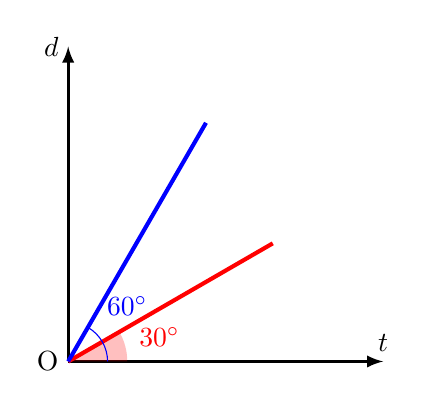
\begin{tikzpicture} 
			\coordinate (O)  at (0,0);
			\coordinate (t) at (4,0);
			\coordinate (d) at (0,4);
			\coordinate (A) at ($(O)+(30:3)$);
			\coordinate (B) at ($(O)+(60:3.5)$);
			\draw[line width=1pt, -latex] (O)--(d);
			\draw[line width=1pt, -latex] (O)--(t);
			\draw[line width=1.5pt, red] (O)--(A);
			\draw[line width=1.5pt, blue] (O)--(B);
			\node[left] at (O) {O};
			\node[above] at (t) {$t$};
			\node[left] at (d) {$d$};
			\tkzFillAngle[size=0.75cm,color=red, fill=red, opacity=0.25](t,O,A);
			\tkzLabelAngle[color=red,pos=1.2](t,O,A){$\SI{30}{\degree}$}
				\tkzMarkAngle[size=0.5cm,color=blue](t,O,B);
		\node[blue] at (0.75,0.7) {$\SI{60}{\degree}$};
		\end{tikzpicture}
	\end{center}
	\choice
	{$\dfrac{3}{1}$}
	{$\dfrac{1}{3}$}
	{$\dfrac{\sqrt{3}}{1}$}
	{$\dfrac{1}{\sqrt{3}}$}
	\loigiai{}
\end{ex}


\Closesolutionfile{ans}
\begin{center}
	\textbf{--- HẾT ---}
\end{center}
	%\tikzstyle{startstop} = [rectangle, rounded corners, minimum width=10cm, minimum height=1.5cm,text centered, draw=black, fill=green!20]
\begin{center}
	\begin{tikzpicture}
		\node (start) [startstop] {\bfseries \text{ÔN TẬP: GIA TỐC - CHUYỂN ĐỘNG THẲNG BIẾN ĐỔI ĐỀU}};
	\end{tikzpicture}
\end{center}
\setcounter{section}{0}
\Opensolutionfile{ans}[ans/G10TUAN4-TN]
% ===================================================================
\begin{ex}
	Gia tốc là đại lượng
	\choice
	{vô hướng, đặc trưng cho sự biến thiên nhanh hay chậm của chuyển động}
	{vô hướng, đặc trưng cho tính không đổi của vận tốc}
	{vector, đặc trưng cho sự biến thiên nhanh hay chậm của chuyển động}
	{\True vector, đặc trưng cho sự biến thiên nhanh hay chậm của vận tốc}
	\loigiai{}
\end{ex}
% ===================================================================
\begin{ex}
	Chọn ý \textbf{sai}. Chuyển động thẳng nhanh dần đều có
	\choice
	{\True vector gia tốc ngược chiều vector vận tốc}
	{vận tốc tức thời là hàm số bậc nhất theo thời gian}
	{toạ độ là hàm số bậc hai theo thời gian}
	{gia tốc không đổi theo thời gian}
	\loigiai{}
\end{ex}
% ===================================================================
\begin{ex}
	Một xe máy đang đứng yên, sau đó khởi động và bắt đầu tăng tốc. Nếu chọn chiều dương cùng chiều chuyển động của xe, nhận xét nào sau đây là \textbf{đúng}? 
	\choice
	{$a<0$, $v<0$}
	{$a>0$, $v<0$}
	{\True $a>0$, $v>0$}
	{$a<0$, $v>0$}
	\loigiai{}
\end{ex}

% ===================================================================
\begin{ex}
Công thức tính quãng đường đi được của vật chuyển động thẳng nhanh dần đều là	
	\choice
	{\True $s=v_0t+\frac{1}{2}at^2$ ($a$ và $v_0$ cùng dấu)}
	{$s=v_0t+\frac{1}{2}at^2$ ($a$ và $v_0$ trái dấu)}
	{$s=at+\frac{1}{2}v_0t^2$ ($a$ và $v_0$ cùng dấu)}
	{$s=at+\frac{1}{2}v_0t^2$ ($a$ và $v_0$ trái dấu)}
	\loigiai{}
\end{ex}
% ===================================================================
\begin{ex}
Tàu hoả đang chuyển động thẳng với tốc độ $\SI{60}{\kilo\meter/\hour}$ thì bị hãm phanh, chuyển động chậm dần đều. Sau khi đi thêm được $\SI{450}{\meter}$ thì tốc độ của tàu chỉ còn $\SI{15}{\kilo\meter/\hour}$. Quãng đường tàu còn đi thêm được đến khi dừng hẳn là	
	\choice
	{$\SI{60}{\meter}$}
	{$\SI{45}{\meter}$}
	{$\SI{15}{\meter}$}
	{\True $\SI{30}{\meter}$}
	\loigiai{}
\end{ex}
% ===================================================================
\begin{ex}
Một ô tô chuyển động chậm dần đều. Sau $\SI{10}{\second}$, tốc độ của ô tô giảm từ $\SI{6}{\meter/\second}$ còn $\SI{4}{\meter/\second}$. Quãng đường ô tô đi được trong khoảng thời gian $\SI{10}{\second}$ đó là	
	\choice
	{$\SI{70}{\meter}$}
	{$\SI{50}{\meter}$}
	{$\SI{40}{\meter}$}
	{\True $\SI{100}{\meter}$}
	\loigiai{}
\end{ex}
% ===================================================================
\begin{ex}
Một ô tô đang chuyển động với tốc độ $\SI{10}{\meter/\second}$ thì bắt đầu tăng tốc, chuyển động nhanh dần đều. Sau $\SI{20}{\second}$ kể từ khi tăng tốc, ô tô đạt tốc độ $\SI{14}{\meter/\second}$. Sau $\SI{50}{\second}$ kể từ lúc tăng tốc, gia tốc và vận tốc của ô tô lần lượt là	
	\choice
	{$\SI{0.2}{\meter/\second^2}$ và $\SI{18}{\meter/\second}$}
	{\True $\SI{0.2}{\meter/\second^2}$ và $\SI{20}{\meter/\second}$}
	{$\SI{0.4}{\meter/\second^2}$ và $\SI{38}{\meter/\second}$}
	{$\SI{0.1}{\meter/\second^2}$ và $\SI{28}{\meter/\second}$}
	\loigiai{}
\end{ex}
% ===================================================================
\begin{ex}
	Một vật chuyển động thẳng có quãng đường đi trong một giai đoạn phụ thuộc thời gian dạng $s=-t^2+3t$ ($s$ đo bằng $\si{\meter}$; $t$ đo bằng giây). Biểu thức vận tốc của vật theo thời gian trong giai đoạn này được xác định bởi
	\choice
	{$v=3+2t$}
	{$v=2-3t$}
	{$v=3-t$}
	{\True $v=3-2t$}
	\loigiai{}
\end{ex}

% ===================================================================
\begin{ex}
Một xe chuyển động trên đường thẳng với biểu thức toạ độ phụ thuộc thời gian: $x=0,4t^2+2t+1$ ($x$ tính bằng $\si{\meter}$; $t$ tính bằng $\si{\second}$). Vận tốc của xe tại thời điểm $t=\SI{5}{\second}$ là
	\choice
	{$\SI{10.4}{\meter/\second}$}
	{$\SI{4.0}{\meter/\second}$}
	{$\SI{5.0}{\meter/\second}$}
	{\True $\SI{6.0}{\meter/\second}$}
	\loigiai{}
\end{ex}

% ===================================================================
\begin{ex}
Một ô tô đang chạy với tốc độ $\SI{10}{\meter/\second}$ trên đoạn đường thẳng thì người lái xe tăng ga và ô tô chuyển động nhanh dần đều. Sau một khoảng thời gian, ô tô đạt tốc độ $\SI{15}{\meter/\second}$. Tốc độ trung bình của ô tô trong khoảng thời gian đó là	
	\choice
	{\True $\SI{12.5}{\meter/\second}$}
	{$\SI{9.5}{\meter/\second}$}
	{$\SI{21}{\meter/\second}$}
	{$\SI{2.5}{\meter/\second}$}
	\loigiai{}
\end{ex}
% ===================================================================
\begin{ex}
	Một vật chuyển động thẳng có phương trình toạ độ $x=20t^2+40t+6$ ($\si{\centi\meter}$; $\si{\second}$). Gia tốc và tính chất chuyển động của vật là
	\choice
	{\True $\SI{40}{\centi\meter/\second^2}$; vật chuyển động nhanh dần đều}
	{$\SI{40}{\centi\meter/\second^2}$; vật chuyển động chậm dần đều}
	{$\SI{20}{\centi\meter/\second^2}$; vật chuyển động nhanh dần đều}
	{$\SI{20}{\centi\meter/\second^2}$; vật chuyển động chậm dần đều}
	\loigiai{}
\end{ex}
% ===================================================================
\begin{ex}
	Lúc $\SI{1}{\hour}$, một xe máy qua A với tốc độ $\SI{10}{\meter/\second}$, chuyển động nhanh dần đều với gia tốc $\SI{1}{\meter/\second^2}$ đuổi theo một xe đạp đang chuyển động nhanh dần đều qua B với tốc độ đầu là $\SI{2}{\meter/\second}$ và với gia tốc $\SI{0.5}{\meter/\second^2}$. Sau $\SI{20}{\second}$ thì xe máy đuổi kịp xe đạp. Khoảng cách AB là
	\choice
	{$\SI{360}{\meter}$}
	{$\SI{160}{\meter}$}
	{$\SI{165}{\meter}$}
	{\True $\SI{260}{\meter}$}
	\loigiai{}
\end{ex}
% ===================================================================
\begin{ex}
	Hai người đi xe đạp khởi hành cùng 1 lúc và đi ngược chiều nhau. Người thứ nhất có tốc độ đầu là $\SI{18}{\kilo\meter/\hour}$ và chuyển động chậm dần đều với gia tốc có độ lớn $\SI{20}{\centi\meter/\second^2}$. Người thứ 2 có tốc độ đầu là $\SI{5.4}{\kilo\meter/\hour}$ và chuyển động nhanh dần đều với gia tốc có độ lớn $\SI{0.2}{\meter/\second^2}$. Khoảng cách ban đầu giữa hai người là $\SI{130}{\meter}$. Sau bao lâu 2 người sẽ gặp nhau và gặp nhau ở vị trí nào?
	\choice
	{\True Sau $\SI{20}{\second}$, cách A đoạn $\SI{60}{\kilo\meter}$}
	{Sau $\SI{17.5}{\second}$, cách A đoạn $\SI{56.9}{\kilo\meter}$}
	{Sau $\SI{20}{\second}$, cách B đoạn $\SI{60}{\kilo\meter}$}
	{Sau $\SI{17.5}{\second}$, cách B đoạn $\SI{56.9}{\kilo\meter}$}
	\loigiai{}
\end{ex}
% ===================================================================
\begin{ex}
	Một vật chuyển động trên đường thẳng có đồ thị vận tốc - thời gian như hình vẽ. Quãng đường vật đi được trong $\SI{400}{\second}$ là 
	\begin{center}
		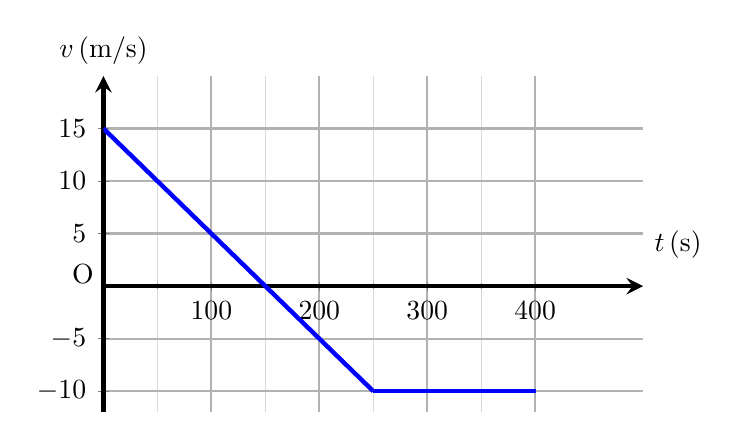
\begin{tikzpicture}  
			\begin{axis}[  ultra thick,yscale=0.75,
				xmin=0,  
				xmax=500,  
				xtick={0,100,...,400},
				ytick={-10,-5,...,15},
				minor x tick num=1,
				minor y tick num=0,
				ymin=-12,  
				ymax=20, 
				samples=300,
				axis lines=center, 
				grid style={step=1, line width =0.4pt, color=gray!30!white},
				grid=both,
				major grid style={line width=0.8pt,gray!60!white},
				xlabel=$\xsi{t}{\left(\si{\second}\right)}$, 		ylabel=$\xsi{v}{\left(\si{\meter/\second}\right)}$,
				every axis y label/.style={at=(current axis.above origin),anchor=south},  
				every axis x label/.style={at=(current axis.right of origin),anchor=west},  ]
				\addplot [ultra thick, blue, smooth, domain=0:250] {15-0.1*x};  
				\addplot [ultra thick, blue, smooth, domain=250:400] {-10};
			 
			\end{axis}  
			\node[below left] at (0,2) {O};
		\end{tikzpicture}
	\end{center}
	\choice
	{$\SI{4625}{\meter}$}
	{\True $\SI{3125}{\meter}$}
	{$\SI{4250}{\meter}$}
	{$\SI{2625}{\meter}$}
	\loigiai{}
\end{ex}
% ===================================================================
\begin{ex}
Một vật chuyển động thẳng có đồ thị vận tốc theo thời gian như hình vẽ. Quãng đường vật đi được trong giai đoạn chuyển động chậm dần đều là	
\begin{center}
	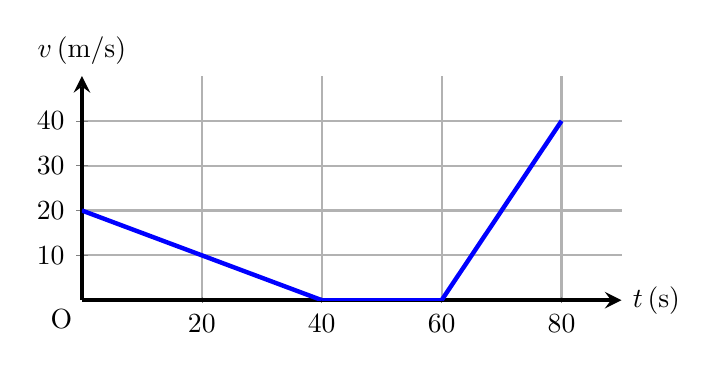
\begin{tikzpicture}  
		\begin{axis}[  ultra thick,yscale=0.5,
			xmin=0,  
			xmax=90,  
			xtick={0,20,...,80},
			ytick={0,10,...,40},
			minor x tick num=0,
			minor y tick num=0,
			ymin=0,  
			ymax=50, 
			samples=300,
			axis lines=center, 
			grid style={step=1, line width =0.4pt, color=gray!30!white},
			grid=both,
			major grid style={line width=0.8pt,gray!60!white},
			xlabel=$\xsi{t}{\left(\si{\second}\right)}$, 		ylabel=$\xsi{v}{\left(\si{\meter/\second}\right)}$,
			every axis y label/.style={at=(current axis.above origin),anchor=south},  
			every axis x label/.style={at=(current axis.right of origin),anchor=west},  ]
			\addplot [ultra thick, blue, smooth, domain=0:40] {20-0.5*x};  
			\addplot [ultra thick, blue, smooth, domain=40:60] {0};
			\addplot [ultra thick, blue, smooth, domain=60:80] {2*(x-60)};
			
		\end{axis}  
	\node[below left] at (0,0) {O}; 
	\end{tikzpicture}
\end{center}
	\choice
	{$\SI{600}{\meter}$}
	{$\SI{800}{\meter}$}
	{$\SI{200}{\meter}$}
	{\True $\SI{400}{\meter}$}
	\loigiai{}
\end{ex}







\Closesolutionfile{ans}
\begin{center}
	\textbf{--- HẾT ---}
\end{center}
	%\setcounter{section}{0}
\begin{center}
	\textbf{\large BẢNG ĐÁP ÁN}
\end{center}
\section{}
\inputansbox{10}{ans/G10C1TN}
\section{}
\inputansbox[2]{2}{ans/G10C1TF}
\section{}
\inputansbox[3]{6}{ans/G10C1TL}\newpage
%	\tikzstyle{startstop} = [rectangle, rounded corners, minimum width=10cm, minimum height=1.5cm,text centered, draw=black, fill=green!20]
\begin{center}
	\begin{tikzpicture}
		\node (start) [startstop] {\bfseries \text{ÔN TẬP: CHƯƠNG MỞ ĐẦU}};
	\end{tikzpicture}
\end{center}
\section{Câu trắc nghiệm nhiều phương án lựa chọn}
\textit{Thí sinh trả lời từ câu 1 đến câu 24. Mỗi câu hỏi thí sinh chọn một phương án}
\setcounter{ex}{0}
\Opensolutionfile{ans}[ans/G10C1TN]
% ===================================================================
\begin{ex}
	Đối tượng nghiên cứu của vật lí là gì?
	\choice
	{Các dạng vận động và tương tác của vật chất}
	{Quy luật tương tác của các dạng năng lượng}
	{\True Các dạng vận động của vật chất và năng lượng}
	{Quy luật vận động, phát triển của sự vật - hiện tượng}
	\loigiai{}
\end{ex}
% ===================================================================
\begin{ex}
Lĩnh vực nghiên cứu nào sau đây là của vật lí?	
	\choice
	{Nghiên cứu về sự thay đổi của các chất khi kết hợp với nhau}
	{Nghiên cứu sự phát triển của vi khuẩn}
	{Nghiên cứu về sự hình thành và phát triển của các tầng lớp, giai cấp trong xã hội}
	{\True Nghiên cứu về các dạng chuyển động và các dạng năng lượng khác nhau}
	\loigiai{}
\end{ex}
% ===================================================================
\begin{ex}
	Thành tựu nghiên cứu nào sau đây của Vật lí được coi là có vai trò quan trọng trong việc mở đầu cho cuộc cách mạng công nghệ lần thứ nhất?
	\choice
	{Nghiên cứu về lực vạn vật hấp dẫn}
	{\True Nghiên cứu về nhiệt động lực học}
	{Nghiên cứu về cảm ứng điện từ}
	{Nghiên cứu về thuyết tương đối}
	\loigiai{}
\end{ex}
% ===================================================================
\begin{ex}
	Trong các hoạt động dưới đây, hoạt động nào tuân thủ nguyên tắc an toàn khi sử dụng điện?
	\choice
	{Sửa chữa điện khi chưa ngắt nguồn điện}
	{Chạm tay trực tiếp vào ổ điện, dây điện trần hoặc dây dẫn điện bị hở}
	{Đến gần nhưng không tiếp xúc với các máy biến thế và lưới điện cao áp}
	{\True Kiểm tra mạch có điện bằng bút thử điện}
	\loigiai{}
\end{ex}
% ===================================================================
\begin{ex}
	Trong các hoạt động dưới đây, hoạt động nào tuân thủ nguyên tắc an toàn khi làm việc với các nguồn phóng xạ?
	\choice
	{Ăn uống, trang điểm trong phòng làm việc có chứa chất phóng xạ}
	{\True Sử dụng phương tiện phòng hộ cá nhân như quần áo phòng hộ, mũ, găng tay, áo chì, \dots}
	{Đổ rác thải phóng xạ tại các khu tập trung rác thải sinh hoạt}
	{Dùng hộp chứa bằng vật liệu thuỷ tinh để đựng chất phóng xạ}
	
	\loigiai{}
\end{ex}
% ===================================================================
\begin{ex}
	Công nghệ chất bán dẫn liên tục phá vỡ các rào cản để có thể tạo ra những con chip nhỏ hơn, nhanh hơn, mạnh hơn và tiết kiệm điện năng hơn. Vừa mới đây, IBM tuyên bố đã tạo ra một con chip $\SI{2}{\nano\meter}$.	Trong khi đó, kích thước trung bình của một gạo là $\SI{6}{\milli\meter}$. So với hạt gạo, con chip trên nhỏ hơn khoảng bao nhiêu lần?
	\begin{center}
		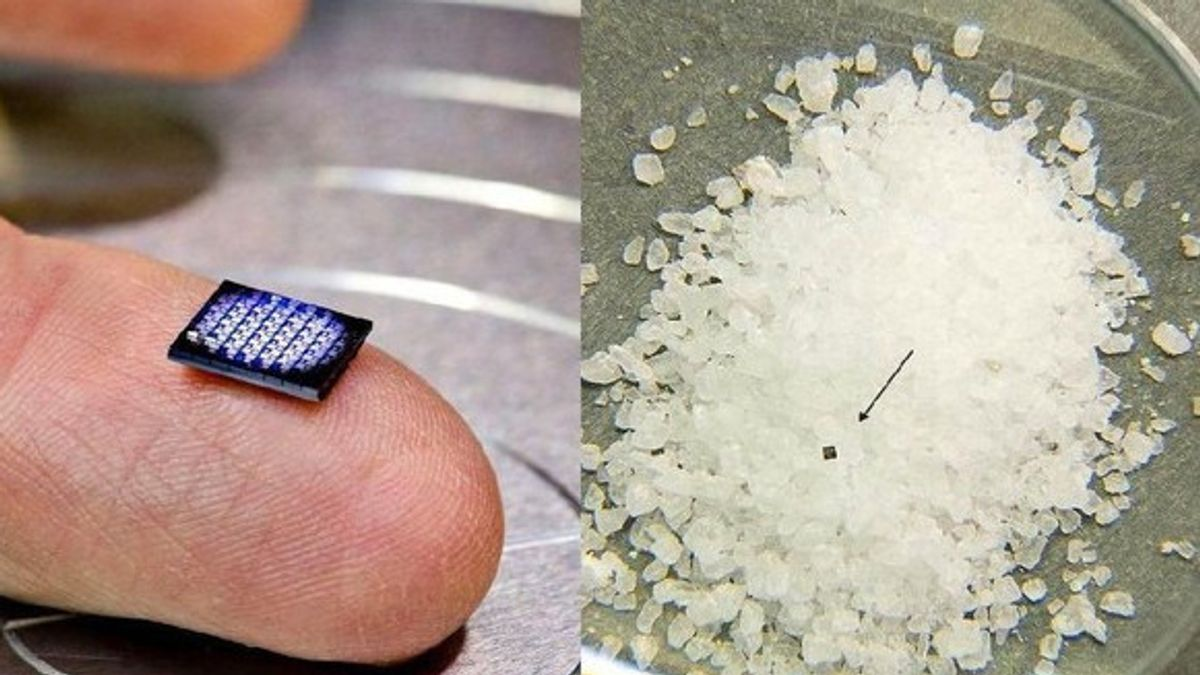
\includegraphics[width=0.4\linewidth]{figs/G10-CHUONG1-6}
		\captionof{figure}{So sánh kích thước chip $\SI{2}{\nano\meter}$ của IBM với các hạt gạo vỡ}
	\end{center}
	\choice
	{$3\cdot10^9$ lần}
	{\True $3\cdot10^6$ lần}
	{$3000$ lần}
	{$0,003$ lần}
	\loigiai{}
\end{ex}
% ===================================================================
\begin{ex}
	Chọn đáp án có từ /cụm từ thích hợp để hoàn thành bảng sau:
	\begin{center}
		\begin{tabular}{|c|c|c|}
			\hline
			\thead{Đơn vị} & \thead{Kí hiệu} & \thead{Đại lượng }\\
			\hline
			kelvin & (1) & (2)\\
			\hline
			ampe & $\si{\ampere}$ & (3)\\
			\hline
			candela & $\si{\candela}$ & (4)\\
			\hline
		\end{tabular}
	\end{center}
	\choice
	{(1) $\si{\kelvin}$; (2) Khối lượng; (3) Cường độ dòng điện; (4) Lượng chất}
	{\True (1) $\si{\kelvin}$; (2) Nhiệt độ; (3) Cường độ dòng điện; (4) Cường độ ánh sáng}
	{(1) $\si{\kelvin}$; (2) Nhiệt độ; (3) Cường độ dòng điện; (4) Lượng chất}
	{(1) $\si{\kelvin}$; (2) Khối lượng; (3) Cường độ dòng điện; (4) Cường độ ánh sáng}
	\loigiai{}
\end{ex}
% ===================================================================
\begin{ex}
	Đơn vị nào sau đây không thuộc thứ nguyên $L$ [Chiều dài]?
	\choice
	{Dặm}
	{Hải lí}
	{Năm ánh sáng}
	{\True Lạng}
	\loigiai{}
\end{ex}
% ===================================================================
\begin{ex}
	Chọn đáp án có từ/cụm từ thích hợp để hoàn thành các câu sau:
	\begin{itemize}
		\item[-] Các số hạng trong phép cộng (hoặc trừ) phải có cùng (1) \dots và nên chuyển về cùng (2) \dots.
		\item[-] (3) \dots của một biểu thức vật lí phải có cùng thứ nguyên.
	\end{itemize}
	\choice
	{(1) đơn vị; (2) thứ nguyên; (3)  Đại lượng}
	{(1) thứ nguyên; (2) đại lượng; (3) Hai vế}
	{(1) đơn vị; (2) đại lượng; (3) Hai vế}
	{\True (1) thứ nguyên; (2) đơn vị; (3) Hai vế}
	\loigiai{}
\end{ex}
% ===================================================================
\begin{ex}
	Trong các phép đo dưới đây, đâu là phép đo trực tiếp?
	\begin{enumerate}[label=(\arabic*)]
		\item Dùng thước đo chiều cao.
		\item Dùng cân đo cân nặng.
		\item Dùng cân và ca đong đo khối lượng riêng của nước.
		\item Dùng đồng hồ và cột cây số đo tốc độ của người lái xe.
	\end{enumerate}
	\choice
	{\True (1), (2)}
	{(1), (2), (4)}
	{(2), (3), (4)}
	{(2), (4)}
	\loigiai{}
\end{ex}
% ===================================================================
\begin{ex}
	Đáp án nào sau đây có 1 đơn vị cơ bản và 1 đơn vị dẫn xuất?
	\choice
	{mét, kilogram}
	{pascal, joule}
	{candela, kelvin}
	{\True newton, mol}
	\loigiai{}
\end{ex}


% ===================================================================
\begin{ex}
		Đại lượng đặc trưng cho tính chất nhanh hay chậm của chuyển động là 
	\choice
	{toạ độ}
	{gia tốc}
	{quãng đường đi}
	{\True tốc độ}
	\loigiai{}
\end{ex}
% ===================================================================
\begin{ex}
	Khi nhìn vào tốc kế của ô tô đang chạy, số chỉ trên tốc kế cho ta biết
	\choice
	{gia tốc tức thời của ô tô}
	{vận tốc tức thời của ô tô}
	{\True tốc độ tức thời của ô tô}
	{tốc độ trung bình của ô tô}
	\loigiai{}
\end{ex}
% ===================================================================
\begin{ex}
	Đâu là cách viết kết quả đo \textbf{đúng}?
	\choice
	{$A=\overline{A}+\Delta A$}
	{$A=\overline{A}-\Delta A$}
	{\True $A=\overline{A}\pm\Delta A$}
	{$A=\overline{A}:\Delta A$}
	\loigiai{}
\end{ex}

% ===================================================================
\begin{ex}
	Giá trị nào sau đây có 2 chữ số có nghĩa (CSCN)?
	\choice
	{\True $\SI{210}{\meter}$}
	{$\SI{20}{\meter}$}
	{$\SI{0.02}{\meter}$}
	{$\SI{201}{\meter}$}
	\loigiai{}
\end{ex}
% ===================================================================
\begin{ex}
Sai số tương đối của đại lượng $A$ được tính bởi công thức	
	\choice
	{\True $\delta A=\dfrac{\Delta A}{\overline{A}}\cdot\SI{100}{\percent}$}
	{$\overline{\Delta A}=\dfrac{\Delta A_1+\Delta A_2+\dots+\Delta A_n}{n}$}
	{$A=\overline{A}\pm\Delta A$}
	{$\delta A=\dfrac{\overline{A}}{\Delta A}$}
	\loigiai{}
\end{ex}

% ===================================================================
\begin{ex}
Một học sinh dùng thước đo chiều dài của chiếc bút chì như hình bên dưới. Nếu lấy sai số dụng cụ bằng 1 nửa độ chia nhỏ nhất thì sai số hệ thống trong phép đo trên là	
\begin{center}
	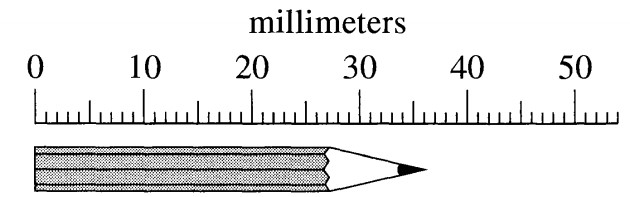
\includegraphics[width=0.4\linewidth]{../figs/G10-CHUONG1-1}
\end{center}
	\choice
	{$\SI{1}{\milli\meter}$}
	{\True $\SI{0.5}{\milli\meter}$}
	{$\SI{1}{\centi\meter}$}
	{$\SI{0.5}{\milli\meter}$}
	\loigiai{}
\end{ex}

% ===================================================================
\begin{ex}
	Một bánh xe có bán kính $R=\xsi{10\pm0,5}{\centi\meter}$. Sai số tương đối của chu vi bánh xe là
	\choice
	{$\SI{0.05}{\percent}$}
	{\True $\SI{5}{\percent}$}
	{$\SI{10}{\percent}$}
	{$\SI{25}{\percent}$}
	\loigiai{
$$\delta R=\dfrac{\Delta R}{\overline{R}}\cdot\SI{100}{\percent}=\SI{5}{\percent}.$$	
}
\end{ex}
% ===================================================================
\begin{ex}
	Thứ nguyên của vận tốc là
	\choice
	{$LT$}
	{$L^{-1}T$}
	{$L^{-1}T^{-1}$}
	{\True $LT^{-1}$}
	\loigiai{
\begin{eqnarray*}
	v&=&\dfrac{s}{t}\\
	\Rightarrow \left[v\right]&=&\dfrac{\left[s\right]}{\left[t\right]}=LT^{-1}.
\end{eqnarray*}	
}
\end{ex}
% ===================================================================
\begin{ex}
	Cho thứ nguyên của trọng lượng là $MLT^{-2}$. Thứ nguyên của trọng lượng riêng là
	\choice
	{$MLT^{-1}$}
	{$MLT^{-2}$}
	{$ML^{-2}T^{-1}$}
	{\True $ML^{-2}T^{-2}$}
	\loigiai{
\begin{eqnarray*}
	d&=&\dfrac{P}{V}\\
	\Rightarrow \left[d\right]&=&\dfrac{\left[P\right]}{\left[V\right]}\\
	\Leftrightarrow \left[d\right]&=&\dfrac{MLT^{-2}}{L^3}=ML^{-2}T^{-2}.
\end{eqnarray*}	
}
\end{ex}
% ===================================================================
\begin{ex}
Một xe xuất phát từ lúc 7 giờ 15 phút sáng từ thành phố M, chuyển động thẳng đều tới thành phố N, cách thành phố M $\SI{90}{\kilo\meter}$. Biết tốc độ của xe là $\SI{60}{\kilo\meter/\hour}$, xe đến thành phố N lúc	
	\choice
	{9 giờ 45 phút}
	{8 giờ 30 phút}
	{9 giờ 30 phút}
	{\True 8 giờ 45 phút}
	\loigiai{
Thời gian để xe đi từ M đến N:
$$\Delta t=\dfrac{s}{v}=\SI{1.5}{\hour}.$$
Thời điểm xe đến N:
$$t=\SI{7}{\hour}\SI{15}{\minute}+\Delta t=\SI{8}{\hour}\SI{45}{\minute}.$$	
}
\end{ex}
% ===================================================================
\begin{ex}
	Một vận động viên chạy cự li $\SI{600}{\meter}$ mất $\SI{74.75}{\second}$. Tốc độ trung bình của vận động viên đó là
	\choice
	{\True $\SI{8.03}{\meter/\second}$}
	{$\SI{9.03}{\meter/\second}$}
	{$\SI{10.03}{\meter/\second}$}
	{$\SI{11.03}{\meter/\second}$}
	\loigiai{
Tốc độ trung bình của vận động viên:
$$v_\text{tb}=\dfrac{s}{\Delta t}=\SI{8.03}{\meter/\second}.$$	
}
\end{ex}
% ===================================================================
\begin{ex}
	Một người bơi dọc theo chiều dài $\SI{55}{\meter}$ của bể bơi hết $\SI{50}{\second}$ rồi quay về lại chỗ xuất phát trong $\SI{60}{\second}$. Trong suốt quãng đường đi và về vận tốc trung bình của người đó là
	\choice
	{\True $\SI{0}{\meter/\second}$}
	{$\SI{1.0}{\meter/\second}$}
	{$\SI{1.1}{\meter/\second}$}
	{$\SI{2.0}{\meter/\second}$}
	\loigiai{
Vì điểm đầu của quĩ đạo chuyển động trùng với điểm cuối nên $d=0\Rightarrow v=0$.	
}
\end{ex}

% ===================================================================
\begin{ex}
	Hình bên là đồ thị toạ độ - thời gian của một chiếc xe máy đang chạy trên đường thẳng. Xe này có tốc độ là
	\begin{center}
		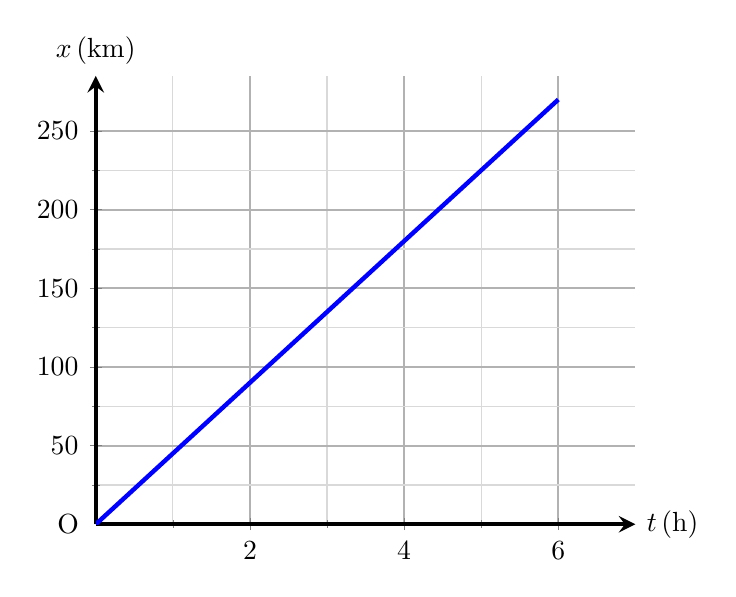
\begin{tikzpicture}  
			\begin{axis}[  ultra thick,
				xmin=0,  
				xmax=7,  
				xtick={0,2,...,6},
				ytick={0,50,...,250},
				minor x tick num=1,
				minor y tick num=1,
				ymin=0,  
				ymax=285, 
				samples=300,
				axis lines=center, 
				grid style={step=1, line width =0.4pt, color=gray!30!white},
				grid=both, %giới hạn ô lưới
				major grid style={line width=0.8pt,gray!60!white},
				xlabel=$\xsi{t}{\left(\si{\hour}\right)}$, 		ylabel=$\xsi{x}{\left(\si{\kilo\meter}\right)}$,
				every axis y label/.style={at=(current axis.above origin),anchor=south},  
				every axis x label/.style={at=(current axis.right of origin),anchor=west},  ] 
				\addplot [ultra thick, blue, smooth, domain=0:6] {45*x}; 
			\end{axis} 
		\node at (-0.35,0) {O}; 
		\end{tikzpicture}
		
	\end{center}
	\choice
	{\True $\SI{45}{\kilo\meter/\hour}$}
	{$\SI{43.75}{\kilo\meter/\hour}$}
	{$\SI{45.45}{\kilo\meter/\hour}$}
	{$\SI{50}{\kilo\meter/\hour}$}
	\loigiai{
Tại $t=\SI{5}{\hour}$ thì $x=\SI{225}{\kilo\meter}$:
$$\left|v\right|=\left|\dfrac{\Delta x}{\Delta t}\right|=\SI{45}{\kilo\meter/\hour}.$$	
}
\end{ex}


\Closesolutionfile{ans}
\section{Câu trắc nghiệm đúng/sai} 
\textit{Trong mỗi ý \textbf{a)}, \textbf{b)}, \textbf{c)}, \textbf{d)} ở câu bên dưới, thí sinh chọn đúng hoặc sai}
\setcounter{ex}{0}
\Opensolutionfile{ans}[ans/G10C1TF]
% ===================================================================
\begin{ex}
Một bạn học sinh dùng volt kế để đo hiệu điện thế hai đầu điện trở. Kết quả trong một lần đo được ghi nhận như hình bên dưới.
\begin{center}
	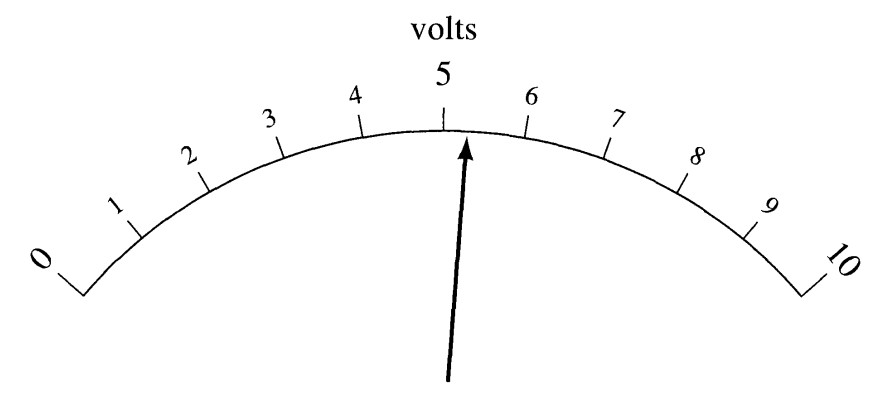
\includegraphics[width=0.6\linewidth]{figs/G10-CHUONG1-2}
\end{center}
	\choiceTF[t]
	{\True Độ chia nhỏ nhất của volt kế trên là $\SI{1}{\volt}$}
	{Kết quả lần đo trên hình nên được đọc là $\SI{5.25}{\volt}$}
	{Có thể hạn chế sai số hệ thống bằng cách thực hiện phép đo nhiều lần}
	{\True Kết quả đo có thể mắc sai số ngẫu nhiên do thao tác của người đo hoặc các yếu tố bên ngoài tác động}
	\loigiai{
\begin{itemchoice}
	\itemch Đúng.
	\itemch Sai. ĐCNN của volt kế là $\SI{1}{\volt}$ nên chỉ có thể đọc được giá trị $\SI{5}{\volt}$ hoặc $\SI{6}{\volt}$. Quan sát chủ quan thấy kim nằm gần vạch $\SI{5}{\volt}$ hơn.
	\itemch Sai. Sai số hệ thống được hạn chế bằng cách dùng dụng cụ có độ chia nhỏ nhất càng nhỏ và hiệu chỉnh dụng cụ đo về 0 trước khi đo.
	\itemch Đúng.
\end{itemchoice}	

}
\end{ex}

\Closesolutionfile{ans}
\section{Câu trắc nghiệm trả lời ngắn} \textit{Thí sinh trả lời từ câu 1 đến câu 6}
\setcounter{ex}{0}
\Opensolutionfile{ans}[ans/G10C1TL]
	% ===============================================================
\begin{ex}
Hố đen là một trong những đối tượng rất đặc biệt trong vũ trụ. Nguồn gốc ra đời của hố đen bắt nguồn từ sự suy sụp hấp dẫn của một vật thể khối lượng rất lớn vào một điểm kỳ dị và tạo ra quanh nó một vùng không - thời gian cong vô hạn, nơi mà không thứ gì có thể thoát ra từ đó, kể cả ánh sáng. 
\begin{center}
	\begin{tabular}{M{7.5cm}M{7.5cm}}
		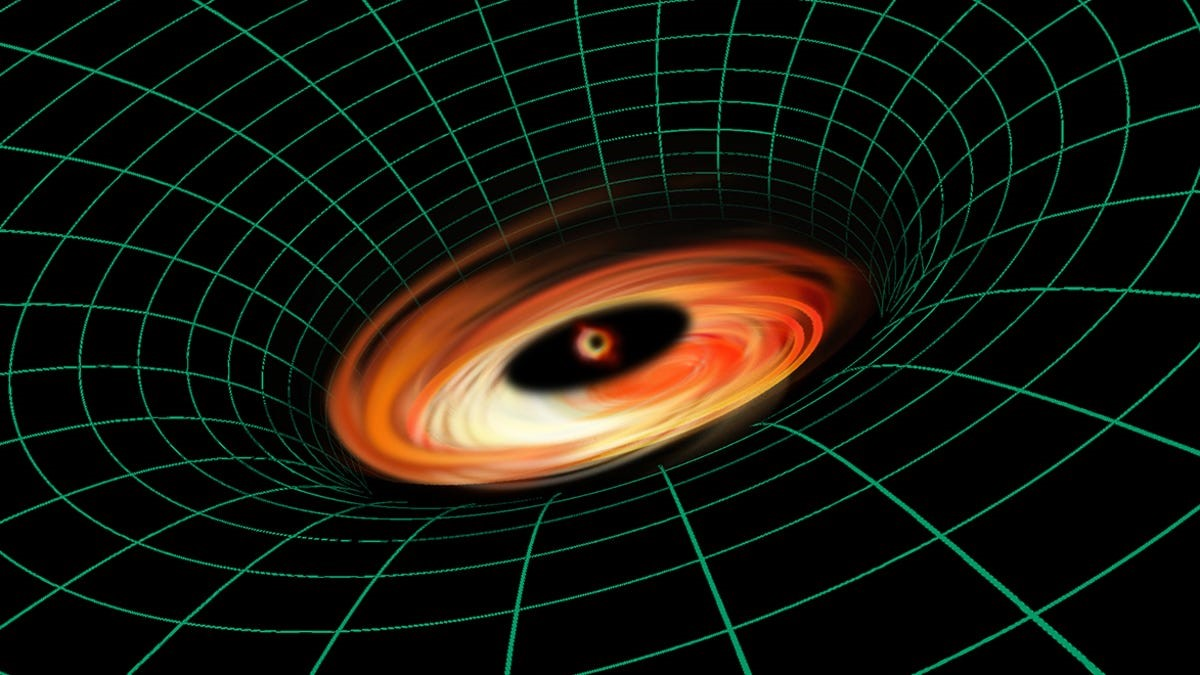
\includegraphics[width=0.7\linewidth]{figs/G10-CHUONG1-4}
		&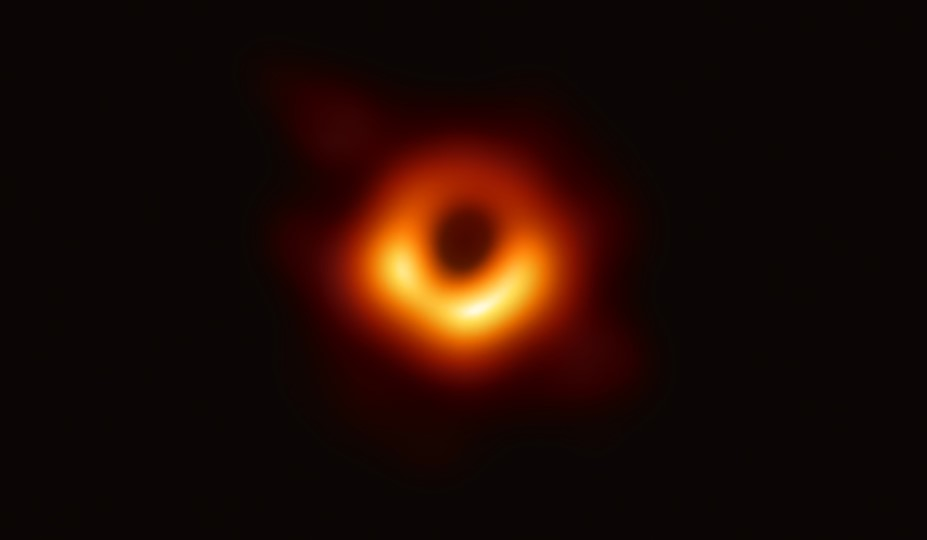
\includegraphics[width=0.7\linewidth]{figs/G10-CHUONG1-5}\\
		\textit{Minh hoạ hố đen làm cong không - thời gian}& \textit{Ảnh hố đen chụp bởi Kính viễn vọng chân trời sự kiện (EHT) và công bố năm 2019} 
	\end{tabular}
\end{center}
Theo nhà vật lí học người Đức Karl Schwarzschild, một vật thể có kích thước bằng với bán kính giới hạn (bán kính Schwarzschild) thì nó sẽ trở thành một hố đen. Bán kính  Schwarzschild được cho bởi công thức:
$$R_S=\dfrac{2GM}{c^2}$$
Trong đó:
\begin{itemize}
	\item $R_S$ là bán kính hấp dẫn Schwarzschild;
	\item $G$ là hằng số hấp dẫn;
	\item $M$ là khối lượng vật thể;
	\item $c$ là tốc độ ánh sáng trong chân không.
\end{itemize}
Trong công thức trên, hằng số hấp dẫn có thứ nguyên là $L^\alpha M^{-\beta}T^{-\gamma}$. Với $\alpha$, $\beta$, $\gamma$ là các số nguyên dương. Xác định giá trị của $\alpha\beta\gamma$.

	\shortans{312 }
	\loigiai{
		Ta có:
		$$G=\dfrac{1}{2}\dfrac{R_Sc^2}{M}.$$
		Phân tích thứ nguyên:
		$$\left[G\right]=\dfrac{\left[R_S\right]\times\left[c\right]^2}{\left[M\right]}=\dfrac{L\times\left(LT^{-1}\right)^2}{M}=L^3M^{-1}T^{-2}\Rightarrow \begin{cases}
			\alpha=3\\
			\beta=1\\
			\gamma=2
		\end{cases}.$$
	}
\end{ex}
	% ===============================================================
\begin{ex}
	Một nhóm học sinh đo được hiệu điện thế giữa hai đầu một điện trở là $U=\xsi{\left(10,0\pm0,3\right)}{\volt}$ và cường độ dòng điện qua điện trở là $I=\xsi{\left(1,3\pm0,2\right)}{\ampere}$. Tính sai số tương đối trong phép đo điện trở \textit{(Kết quả tính theo đơn vị $\si{\percent}$ và làm tròn đến 3 CSCN)}.\\
	Cho biết giá trị của điện trở được xác định bởi $R=\dfrac{U}{I}$.
	\shortans{18,4 }
	\loigiai{
		Giá trị điện trở:
		$$R=\dfrac{U}{I}.$$
		Sai số tương đối của phép đo:
		$$\delta R=\left(\dfrac{\Delta U}{\overline{U}}+\dfrac{\Delta I}{\overline{I}}\right)\cdot\SI{100}{\percent}\approx\SI{18.4}{\percent}.$$
	}
\end{ex}
\textit{Dữ kiện sau đây được dùng chung cho câu 3 đến câu 6}\\
Bạn An thực hiện thí nghiệm đo tốc độ chuyển động thẳng với dụng cụ và sơ đồ bố trí thí nghiệm như hình bên dưới.
Trong đó, hai cổng quang điện A và B được đặt cách nhau $\SI{30}{\centi\meter}$ và được nối với đồng hồ đo thời gian hiện số (1) được đặt ở chế độ đo với sai số dụng cụ $\SI{0.01}{\second}$. Độ chia nhỏ nhất của thước đo (5) là $\SI{0.5}{\centi\meter}$.
\begin{center}
	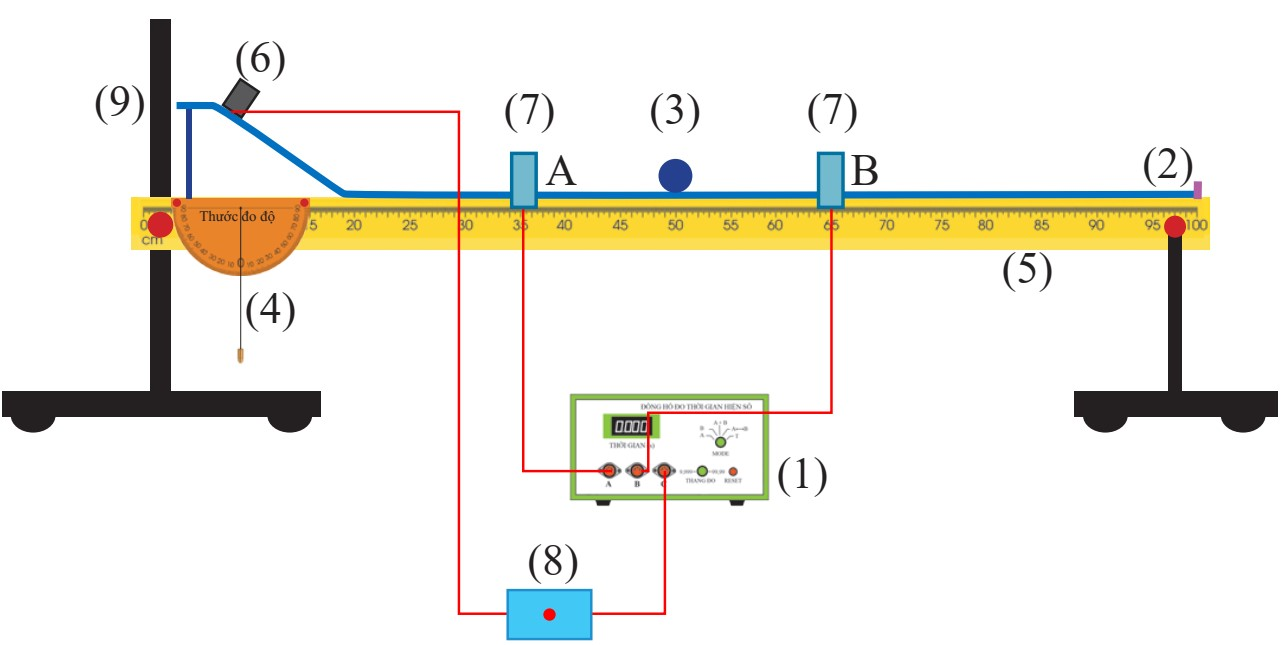
\includegraphics[width=0.75\linewidth]{../figs/G10-CHUONG1-3}
\end{center}
Bạn An thiết đặt đồng hồ đo thời gian hiện số ở chế độ A$\leftrightarrow$B để đo thời gian viên bi chuyển động kể từ khi chắn qua cổng quang A đến khi qua cổng quang B. Sau 5 lần đo, An ghi nhận được các giá trị thời gian chuyển động của viên bi như bảng bên dưới:
\begin{center}
	\begin{longtable}{|M{4cm}|M{2cm}|M{2cm}|M{2cm}|M{2cm}|M{2cm}|}
		\hline
		\thead{Lần đo}&1&2&3&4&5\\
		\hline
		\thead{Thời gian $\left(\si{\second}\right)$}& 4,75 & 4,68 & 4,73 & 4,68 & 4,70\\
		\hline
	\end{longtable}
\end{center}
\textit{* Lưu ý: Trong các phần tính toán bên dưới, các giá trị trung bình được lấy cùng bậc thập phân với giá trị đo.}
	% ===============================================================
\begin{ex}
Xác định thời gian chuyển động trung bình của viên bi \textit{(Kết quả tính theo đơn vị giây và làm tròn đến 3 CSCN)}.
	\shortans{4,71}
	\loigiai{
		Thời gian chuyển động trung bình của viên bi:
	$$\overline{t}=\dfrac{t_1+t_2+\dots+t_5}{5}=\SI{4.708}{\second}\approx\SI{4.71}{\second}.$$	
	}
\end{ex}
	% ===============================================================
\begin{ex}
Xác định sai số tương đối trong phép đo trên \textit{(Kết quả tính theo đơn vị $\si{\percent}$ và làm tròn đến 3 CSCN)}.
	\shortans{0,85}
	\loigiai{
		\begin{center}
			\begin{longtable}{|M{2cm}|M{4cm}|M{2cm}|}
				\hline
				\thead{Lần đo} & $\xsi{t}{\left(\second\right)}$ &$\xsi{\Delta t}{\left(\second\right)}$\\
				\hline
				1 & 4,75 &0,04 \\
				\hline
				2 & 4,68 & 0,03\\
				\hline
				3 & 4,73 & 0,02\\
				\hline
				4 & 4,68 & 0,03\\
				\hline
				5 & 4,70 & 0,01\\
				\hline
				\thead{TB}&4,71&0,03\\
				\hline
			\end{longtable}
		\end{center}
	Sai số tuyệt đối của phép đo thời gian:
	$$\Delta t=\overline{\Delta t}+\Delta t_{\text{dc}}=\SI{0.03}{\second}+\SI{0.01}{\second}=\SI{0.04}{\second}.$$
Sai số tương đối của phép đo thời gian:
$$\delta t=\dfrac{\Delta t}{\overline{t}}\cdot\SI{100}{\percent}=\dfrac{\SI{0.04}{\second}}{\SI{4.71}{\second}}\cdot\SI{100}{\percent}\approx\SI{0.85}{\percent}.$$}
\end{ex}
	% ===============================================================
\begin{ex}
	Xác định tốc độ trung bình của viên bi trong thí nghiệm trên \textit{(Kết quả tính theo đơn vị $\si{\centi\meter/\second}$ và làm tròn đến 3 CSCN)}.
	\shortans{6,37}
	\loigiai{
		$$\overline{v}=\dfrac{\overline{s}}{\overline{t}}=\dfrac{\SI{30}{\centi\meter}}{\SI{4.71}{\second}}\approx\SI{6.37}{\centi\meter/\second}.$$
	}
\end{ex}
	% ===============================================================
\begin{ex}
	Xác định sai số tuyệt đối trong phép đo tốc độ trung bình của viên bi \textit{(Kết quả tính theo đơn vị $\si{\centi\meter/\second}$ và làm tròn đến 3 CSCN)}.
	\shortans{0,11}
	\loigiai{
		ĐCNN của thước (5) là $\SI{0.5}{\centi\meter}$ nên sai số $\Delta s=\dfrac{\SI{0.5}{\centi\meter}}{2}=\SI{0.25}{\centi\meter}$.\\
		Sai số tuyệt đối trong phép đo tốc độ trung bình:
		$$\dfrac{\Delta v}{\overline{v}}=\dfrac{\Delta s}{\overline{s}}+\dfrac{\Delta t}{\overline{t}}\Rightarrow \Delta v=\left(\dfrac{\Delta s}{\overline{s}}+\dfrac{\Delta t}{\overline{t}}\right)\cdot\overline{v}=\left(\dfrac{\SI{0.25}{\centi\meter}}{\SI{30}{\centi\meter}}+\dfrac{\SI{0.04}{\second}}{\SI{4.71}{\second}}\right)\cdot\left(\SI{6.37}{\centi\meter/\second}\right)\approx\SI{0.11}{\centi\meter}.$$
	}
\end{ex}
\Closesolutionfile{ans}
\begin{center}
	\textbf{--- HẾT ---}
\end{center}
	%\begin{center}\textbf{\color{red}BÀI TẬP BỔ SUNG}\\
	\textbf{Bài 4. CHUYỂN ĐỘNG THẲNG}
\end{center}
% ======================================================================
\begin{ex}
	Lúc $\SI{7}{\hour}$ có một xe khởi hành từ A chuyển động thẳng đều về B với tốc độ $\SI{40}{\kilo\meter/\hour}$. Lúc $\SI{7}{\hour}\SI{30}{\minute}$ một xe khác khởi hành từ B chuyển động thẳng đều về A  với tốc độ $\SI{50}{\kilo\meter/\hour}$. Cho $\mathrm{AB}=\SI{110}{\kilo\meter}$.
	\begin{enumerate}[label=\alph*)]
		\item Xác định vị trí của mỗi xe và khoảng cách giữa chúng lúc $\SI{8}{\hour}$ và lúc $\SI{9}{\hour}$.
		\item Hai xe gặp nhau lúc mấy giờ? Ở đâu?
	\end{enumerate}
	\loigiai{
	\begin{enumerate}[label=\alph*)]
		\item Cách A $\SI{40}{\kilo\meter}$, $\SI{85}{\kilo\meter}$, $\SI{45}{\kilo\meter}$.\\
		Cách A $\SI{80}{\kilo\meter}$, $\SI{35}{\kilo\meter}$, $\SI{45}{\kilo\meter}$.
		\item $\SI{8}{\hour}\SI{30}{\minute}$; cách A $\SI{60}{\kilo\meter}$.
	\end{enumerate}
	}
\end{ex}
% ======================================================================
\begin{ex}
	Hai xe chuyển động trên hai đường vuông góc với nhau, xe A đi về hướng tây với tốc độ $\SI{50}{\kilo\meter/\hour}$, xe B đi về hướng Nam với tốc độ $\SI{30}{\kilo\meter/\hour}$. Vào một thời điểm nào đó xe A và B còn cách giao điểm của hai đường lần lượt là $\SI{4.4}{\kilo\meter}$ và $\SI{4}{\kilo\meter}$, hai xe đang tiến về phía giao điểm. Tìm khoảng cách ngắn nhất giữa hai xe.
	\loigiai{
	$\SI{1.166}{\kilo\meter}$.
	}
\end{ex}
	%\begin{center}\textbf{\color{red}LUYỆN TẬP}\\
	\textbf{Bài 5. CHUYỂN ĐỘNG TỔNG HỢP}
\end{center}
\section{TRẮC NGHIỆM}
\Opensolutionfile{ans}[ans/BAI5-TN]
% ===================================================================
\begin{ex}
Một người đi xe máy từ nhà đến bến xe bus cách nhà $\SI{6}{\kilo\meter}$ về phía Đông. Người đó tiếp tục lên xe bus đi tiếp $\SI{6}{\kilo\meter}$ về phía Bắc. Độ dịch chuyển tổng hợp của người này là	
	\choice
	{$\SI{12}{\kilo\meter}$}
	{$\SI{6}{\kilo\meter}$}
	{\True $\xsi{6\sqrt{2}}{\kilo\meter}$}
	{$\SI{72}{\kilo\meter}$}
	\loigiai{}
\end{ex}
% ===================================================================
\begin{ex}
	Gọi $\vec{v}_{12}$ là vận tốc của vật (1) so với vật (2), $\vec{v}_{23}$ là vận tốc của vật (2) so với vật (3), $\vec{v}_{13}$ là vận tốc của vật (1) so với vật (3). Hệ thức đúng là
	\choice
	{$\vec{v}_{13}=\vec{v}_{12}-\vec{v}_{23}$}
	{$\vec{v}_{13}=\vec{v}_{12}+2\vec{v}_{23}$}
	{\True $\vec{v}_{13}=\vec{v}_{12}+\vec{v}_{23}$}
	{$\vec{v}_{13}=2\vec{v}_{12}+\vec{v}_{23}$}
	\loigiai{}
\end{ex}
% ===================================================================
\begin{ex}
	Một hành khách ngồi trong xe A, nhìn qua cửa sổ thấy xe B bên cạnh và sân ga đều chuyển động như nhau. Như vậy
	\choice
	{xe A đứng yên, xe B chuyển động}
	{\True xe A chạy, xe B đứng yên}
	{xe A và xe B chạy cùng chiều}
	{xe A và xe B chạy ngược chiều}
	\loigiai{}
\end{ex}
% ===================================================================
\begin{ex}
Hai ô tô A và B chạy cùng chiều trên cùng một đoạn đường với tốc độ $\SI{70}{\kilo\meter/\hour}$ và $\SI{65}{\kilo\meter/\hour}$. Tốc độ của ô tô A so với ô tô B bằng	
	\choice
	{$\SI{30}{\kilo\meter/\hour}$}
	{\True $\SI{5}{\kilo\meter/\hour}$}
	{$\SI{135}{\kilo\meter/\hour}$}
	{$\SI{65}{\kilo\meter/\hour}$}
	\loigiai{}
\end{ex}
% ===================================================================
\begin{ex}
	A ngồi trên một toa tàu chuyển động với tốc độ $\SI{15}{\kilo\meter/\hour}$ đang rời ga. B ngồi trên một toa tàu khác chuyển động với tốc độ $\SI{10}{\kilo\meter/\hour}$ đang đi ngược chiều vào ga. Hai đường tàu song song với nhau. Chọn chiều dương là chiều chuyển động của đoàn tàu mà A ngồi. Vận tốc của B đối với A là
	\choice
	{$\SI{-5}{\kilo\meter/\hour}$}
	{$\SI{5}{\kilo\meter/\hour}$}
	{$\SI{25}{\kilo\meter/\hour}$}
	{\True $\SI{-25}{\kilo\meter/\hour}$}
	\loigiai{}
\end{ex}
% ===================================================================
\begin{ex}
Hai bến sông A và B cùng nằm trên một bờ sông, cách nhau $\SI{18}{\kilo\meter}$. Cho biết độ lớn vận tốc của ca nô đối với nước là $u =\SI{16.2}{\kilo\meter/\hour}$ và độ lớn vận tốc của nước đối với bờ sông là $v=\SI{5.4}{\kilo\meter/\hour}$. Thời gian để ca nô chạy xuôi dòng từ A đến B rồi lại chạy ngược dòng trở về A là	
	\choice
	{1 giờ 40 phút}
	{1 giờ 20 phút}
	{\True 2 giờ 30 phút}
	{2 giờ 10 phút}
	\loigiai{}
\end{ex}
% ===================================================================
\begin{ex}
Ô tô A chạy thẳng về hướng Tây với độ lớn vận tốc $\SI{40}{\kilo\meter/\hour}$. Ô tô B chạy thẳng về hướng Bắc với độ lớn vận tốc $\SI{60}{\kilo\meter/\hour}$. Độ lớn vận tốc của ô tô B so với người ngồi trên ô tô A gần giá trị nào nhất sau đây?	
	\choice
	{$\SI{85}{\kilo\meter/\hour}$}
	{$\SI{90}{\kilo\meter/\hour}$}
	{$\SI{65}{\kilo\meter/\hour}$}
	{\True $\SI{75}{\kilo\meter/\hour}$}
	\loigiai{}
\end{ex}
% ===================================================================
\begin{ex}
	Một chiếc xuồng đi xuôi dòng nước từ A đến B mất 4 giờ, còn nếu đi ngược dòng nước từ B đến A mất 5 giờ. Biết vận tốc của dòng nước so với bờ sông là $\SI{4}{\kilo\meter/\hour}$. Quãng đường AB là
	\choice
	{\True $\SI{160}{\kilo\meter}$}
	{$\SI{120}{\kilo\meter}$}
	{$\SI{130}{\kilo\meter}$}
	{$\SI{150}{\kilo\meter}$}
	\loigiai{}
\end{ex}
% ===================================================================
\begin{ex}
	Một người lái xuồng máy cho xuồng chạy ngang con sông rộng $\SI{240}{\meter}$. Mũi xuồng luôn luôn vuông góc với bờ sông, nhưng do nước chảy nên xuồng sang đến bờ bên kia tại một điểm cách bến dự định $\SI{180}{\meter}$ về phía hạ lưu và xuồng đi hết 1 phút. Độ lớn vận tốc của xuồng so với bờ là
	\choice
	{$\SI{8}{\meter/\second}$}
	{$\SI{9}{\meter/\second}$}
	{$\SI{6}{\meter/\second}$}
	{\True $\SI{5}{\meter/\second}$}
	\loigiai{}
\end{ex}
% ===================================================================
\begin{ex}
	Nhà của Bách và trường nằm trên cùng một con đường nên hằng ngày Bách đều đi học bằng xe đạp từ nhà đến trường với tốc độ không đổi bằng $\SI{4}{\meter/\second}$ (khi trời lặng gió). Trong một lần Bách đạp xe từ nhà đến trường, có một cơn gió thổi ngược chiều trong khoảng thời gian $\SI{90}{\second}$ . Hình bên mô tả đồ thị độ dịch chuyển - thời gian của Bách trong 5 phút đầu tiên. Tốc độ của gió so với mặt đất là bao nhiêu?
\begin{center}
		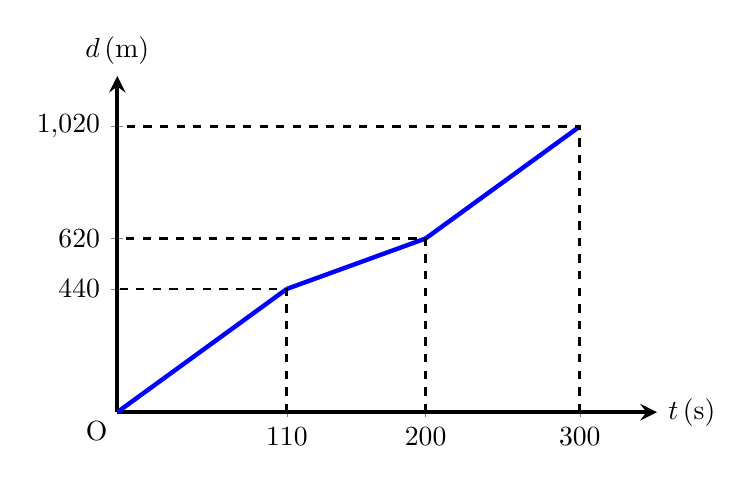
\begin{tikzpicture}  
		\begin{axis}[  ultra thick,yscale=0.75,
			xmin=0,  
			xmax=350,  
			xtick={0,110,200,300},
			ytick={0,440,620,1020},
			minor x tick num=0,
			minor y tick num=0,
			ymin=0,  
			ymax=1200, 
			samples=300,
			axis lines=center, 
			xlabel=$\xsi{t}{\left(\si{\second}\right)}$, 		ylabel=$\xsi{d}{\left(\si{\meter}\right)}$,
			every axis y label/.style={at=(current axis.above origin),anchor=south},  
			every axis x label/.style={at=(current axis.right of origin),anchor=west},  ]
			\addplot [ultra thick, blue, smooth, domain=0:110] {4*x};  
			\addplot [ultra thick, blue, smooth, domain=110:200] {440+2*(x-110)}; 
			\addplot [ultra thick, blue, smooth, domain=200:300] {620+4*(x-200)}; 
			\draw[dashed, line width=1pt] (axis cs: 110,0)--(axis cs:110,440)--(axis cs:0,440);
			\draw[dashed, line width=1pt] (axis cs: 200,0)--(axis cs:200,620)--(axis cs:0,620);
			\draw[dashed, line width=1pt] (axis cs: 300,0)--(axis cs:300,1020)--(axis cs:0,1020);
		\end{axis}  
		\node[below left] at(0,0) {O};
	\end{tikzpicture}
\end{center}
	\choice
	{$\SI{1.2}{\meter/\second}$}
	{$\SI{1.5}{\meter/\second}$}
	{\True $\SI{2}{\meter/\second}$}
	{$\SI{2.5}{\meter/\second}$}
	\loigiai{}
\end{ex}

\Closesolutionfile{ans}
\section{TỰ LUẬN}
\setcounter{ex}{0}
% ======================================================================
\begin{ex}
Một ca nô chạy hết tốc lực trên mặt nước yên lặng có thể đạt $\SI{21,5}{km/h}$. Ca nô này chạy xuôi dòng sông trong 1 giờ rồi quay lại thì phải mất 2 giờ nữa mới về tới vị trí ban đầu. Hãy tính tốc độ của dòng nước.	
	\loigiai{$\SI{7.17}{\kilo\meter/\hour}$}
\end{ex}
% ======================================================================
\begin{ex}
	Một máy bay đang bay theo hướng Bắc với vận tốc $\SI{200}{m/s}$ thì bị gió từ hướng Tây thổi vào với vận tốc $\SI{20}{m/s}$. Xác định vận tốc tổng hợp của máy bay lúc này.
	\loigiai{}
\end{ex}
% ======================================================================
\begin{ex}
	Một người lái tàu vận chuyển hàng hoá xuôi dòng từ sông Đồng Nai đến khu vực cảng Sài Gòn với tốc độ là $\SI{40}{\kilo\meter/\hour}$ so với bờ. Sau khi hoàn thành công việc, lái tàu quay lại sông Đồng Nai theo lộ trình cũ với tốc độ là $\SI{30}{\kilo\meter/\hour}$ so với bờ. Biết rằng chiều và tốc độ của dòng nước đối với bờ không thay đổi trong suốt quá trình tàu di chuyển, ngoài ra tốc độ của tàu so với nước cũng được xem là không đổi. Hãy xác định tốc độ của dòng nước so với bờ.
	\loigiai{$\SI{5}{\kilo\meter/\hour}$}
\end{ex}
% ======================================================================
\begin{ex}
	Một người chèo thuyền qua một con sông rộng $\SI{400}{\meter}$. Muốn cho thuyền đi theo đường AB thì người đó phải luôn hướng mũi thuyền theo hướng AC. Biết thuyền qua sông hết $\SI{8}{\minute} \SI{20}{\second}$ và tốc độ của dòng nước là $\SI{0.6}{\meter/\second}$. Tìm tốc độ của thuyền so với dòng nước.
	\begin{center}
		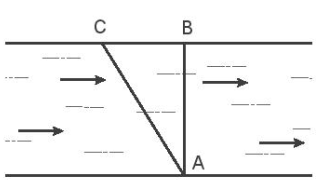
\includegraphics[width=0.35\linewidth]{figs/BAI5-1}
	\end{center}
	\loigiai{$\SI{1}{\meter/\second}$.}
\end{ex}
% ======================================================================
\begin{ex}
	Tại một thời điểm, ở vị trí M trên đoạn đường thẳng có xe máy A chạy qua với tốc độ $\SI{30}{\kilo\meter/\hour}$. Sau 10 phút, cũng tại vị trí M , có xe máy B chạy qua với tốc độ $\SI{40}{\kilo\meter/\hour}$ để đuổi theo xe máy A . Giả sử hai xe máy chuyển động thẳng với tốc độ xem như không đổi.
	\begin{enumerate}[label=\alph*)]
		\item Tính thời gian để xe máy B đuổi kịp xe máy A.
		\item Tính quãng đường mà xe máy A đã đi được đến khi xe máy B đuổi kịp.
	\end{enumerate}
	\loigiai{
	\begin{enumerate}[label=\alph*)]
		\item $\SI{0.5}{\hour}$.
		\item $\SI{15}{\kilo\meter}$.
	\end{enumerate}
	}
\end{ex}
% ======================================================================
\begin{ex}
	Một ô tô đang chạy với vận tốc $v$ theo phương nằm ngang thì người ngồi trong xe trông thấy giọt mưa rơi tạo thành những vạch làm với phương thẳng đứng một góc $\SI{45}{\degree}$. Biết vận tốc rơi của các giọt nước mưa so với mặt đất là $\SI{5}{\meter/\second}$. Tính vận tốc của ô tô.
	\loigiai{$\SI{5}{\meter/\second}$}
\end{ex}
% ======================================================================
\begin{ex}
	Một ca nô chạy ngang qua một dòng sông, xuất phát từ A , hướng mũi về B . Sau $\SI{100}{\second}$, ca nô cập bờ bên kia ở điểm C cách B $\SI{200}{\meter}$. Nếu người lái hướng mũi ca nô theo hướng AD và vẫn giữ tốc độ máy như cũ thì ca nô sẽ cập bờ bên kia tại đúng điểm B. Tìm:
	\begin{center}
		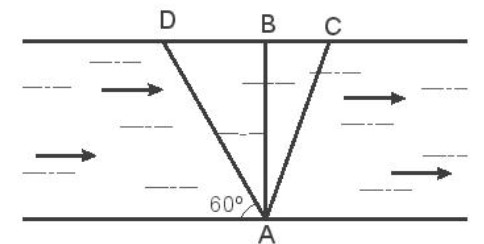
\includegraphics[width=0.35\linewidth]{figs/BAI5-2}
	\end{center}
	\begin{enumerate}[label=\alph*)]
		\item Vận tốc của dòng nước so với bờ sông.
		\item Vận tốc của ca nô so với dòng nước.
		\item Chiều rộng của sông.
	\end{enumerate}
	\loigiai{
	\begin{enumerate}[label=\alph*)]
		\item $\SI{2}{\meter/\second}$.
		\item $\SI{4}{\meter/\second}$.
		\item $\SI{400}{\meter}$.
	\end{enumerate}
	}
\end{ex}
% ======================================================================
\begin{ex}
	Hai xe chuyển động trên hai đường vuông góc với nhau, xe A đi về hướng tây với tốc độ $\SI{50}{\kilo\meter/\hour}$, xe B đi về hướng Nam với tốc độ $\SI{30}{\kilo\meter/\hour}$. Vào một thời điểm nào đó xe A và B còn cách giao điểm của hai đường lần lượt là $\SI{4.4}{\kilo\meter}$ và $\SI{4}{\kilo\meter}$, hai xe đang tiến về phía giao điểm. Tìm khoảng cách ngắn nhất giữa hai xe.\\
	\textit{(Hãy tính bài này bằng 2 cách: dùng phương pháp tọa độ và dùng vận tốc tương đối!!!)}
	\loigiai{
		$\SI{1.166}{\kilo\meter}$.
	}
\end{ex}
\begin{center}
	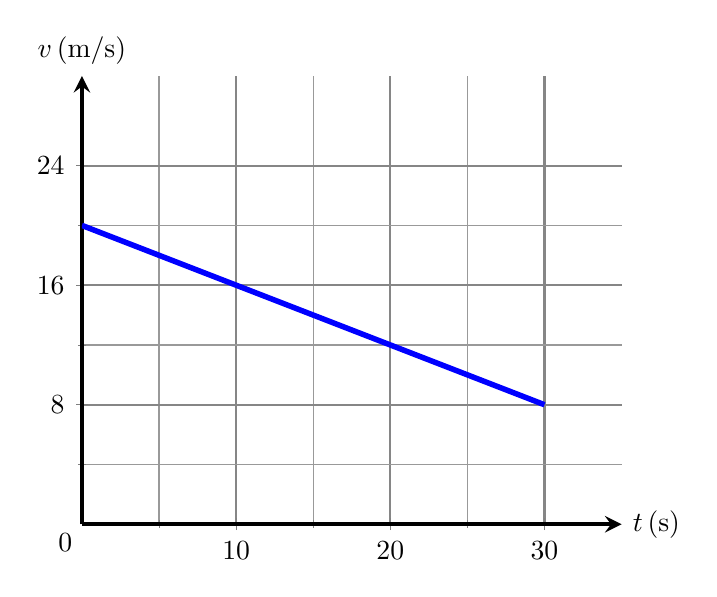
\begin{tikzpicture}  
		\begin{axis}[  ultra thick,
			xmin=0,  
			xmax=35,  
			xtick={0,10,...,30},
			ytick={0,8,...,24},
			minor x tick num=1,
			minor y tick num=1,
			ymin=0,  
			ymax=30, 
			samples=300,
			axis lines=center, 
			grid style={step=1, line width =0.4pt, color=gray!80!white},
			grid=both, %giới hạn ô lưới
			major grid style={line width=0.8pt,gray!95!white},
			xlabel=$\xsi{t}{\left(\si{\second}\right)}$, 		ylabel=$\xsi{v}{\left(\si{\meter/\second}\right)}$,
			every axis y label/.style={at=(current axis.above origin),anchor=south},  
			every axis x label/.style={at=(current axis.right of origin),anchor=west},  ]
			\addplot [line width=2pt, blue, smooth, domain=0:30] {20-0.4*x};  
			\coordinate (O) at (0,0);
		\end{axis}  
		\node[below left] at (O) {0};
	\end{tikzpicture}
\end{center}
\begin{center}
	\textbf{--- HẾT ---}
\end{center}
%	\begin{center}\textbf{\color{red}LUYỆN TẬP}\\
	\textbf{Bài 7. GIA TỐC - CHUYỂN ĐỘNG THẲNG BIẾN ĐỔI ĐỀU}
\end{center}
\section{TRẮC NGHIỆM}
\Opensolutionfile{ans}[ans/BAI7-TN]
% ===================================================================
\begin{ex}
	Một xe máy đang đứng yên, sau đó khởi động và bắt đầu tăng tốc. Nếu chọn chiều dương cùng  chiều chuyển động của xe, nhận xét nào sau đây là đúng? 
	\choice
	{$a<0$, $v<0$}
	{$a>0$, $v<0$}
	{\True $a>0$, $v>0$}
	{$a<0$, $v>0$}
	\loigiai{}
\end{ex}
% ===================================================================
\begin{ex}
	Gia tốc là đại lượng
	\choice
	{\True vector, đặc trưng cho sự biến thiên nhanh hay chậm của vận tốc}
	{vô hướng, đặc trưng cho tính chất nhanh hay chậm của chuyển động}
	{vector, đặc trưng cho tính chất nhanh hay chậm của chuyển động}
	{vô hướng, đặc trưng cho tính sự biến thiên nhanh hay chậm của vận tốc}
	\loigiai{}
\end{ex}
% ===================================================================
\begin{ex}
	Công thức liên hệ giữa độ dịch chuyển, vận tốc và gia tốc của chuyển động nhanh dần đều là
	\choice
	{$v^2-v^2_0=ad$}
	{\True $v^2-v^2_0=2ad$}
	{$v-v_0=2ad$}
	{$v^2_0-v^2=2ad$}
	\loigiai{}
\end{ex}
% ===================================================================
\begin{ex}
	Trong các phương trình mô tả vận tốc $v\ \left(\si{\meter/\second}\right)$ của vật theo thời gian $t\ \left(\si{\second}\right)$ dưới đây, phương trình nào mô tả chuyển động thẳng biến đổi đều?
	\choice
	{$v=7$}
	{$v=6t^2+2t-2$}
	{\True $v=5t-4$}
	{$v=6t^2-2$}
	\loigiai{}
\end{ex}
% ===================================================================
\begin{ex}
Cho các đồ thị độ dịch chuyển - thời gian $\left(d-t\right)$ và vận tốc - thời gian $\left(v-t\right)$ như hình bên dưới. Đồ thị ứng với chuyển động thẳng biến đổi đều là
\begin{center}
	\begin{tabular}{M{4cm}M{4cm}M{4cm}M{4cm}}
		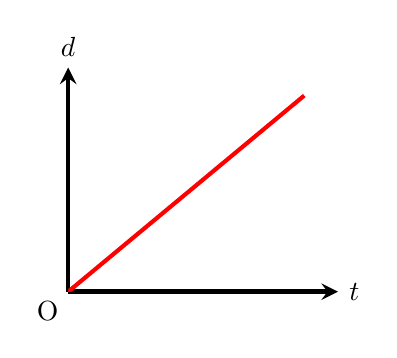
\begin{tikzpicture}  
			\begin{axis}[  ultra thick,scale=0.5,
				xmin=0,  
				xmax=4,  
				ymin=0,  
				ymax=4, 
				samples=300,
				yticklabels=\empty,
				xticklabels=\empty,
				xtick=\empty,
				ytick=\empty,
				axis lines=center, 
				xlabel=$t$, 		ylabel=$d$,
				every axis y label/.style={at=(current axis.above origin),anchor=south},  
				every axis x label/.style={at=(current axis.right of origin),anchor=west},  ]
				\addplot [line width=1.5pt, red, smooth, domain=0:3.5] {x};  
				\coordinate (O) at (0,0);
			\end{axis}  
			\node[below left] at (O) {O};
		\end{tikzpicture}&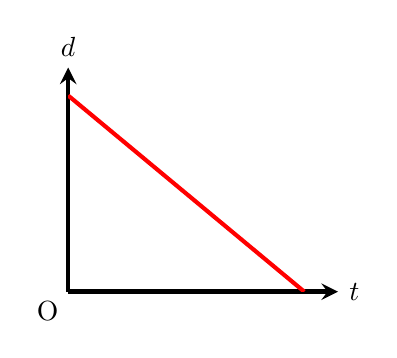
\begin{tikzpicture}  
		\begin{axis}[  ultra thick,scale=0.5,
			xmin=0,  
			xmax=4,  
			ymin=0,  
			ymax=4, 
			samples=300,
			yticklabels=\empty,
			xticklabels=\empty,
			xtick=\empty,
			ytick=\empty,
			axis lines=center, 
			xlabel=$t$, 		ylabel=$d$,
			every axis y label/.style={at=(current axis.above origin),anchor=south},  
			every axis x label/.style={at=(current axis.right of origin),anchor=west},  ]
			\addplot [line width=1.5pt, red, smooth, domain=0:3.5] {3.5-x};  
			\coordinate (O) at (0,0);
		\end{axis}  
		\node[below left] at (O) {O};
		\end{tikzpicture}&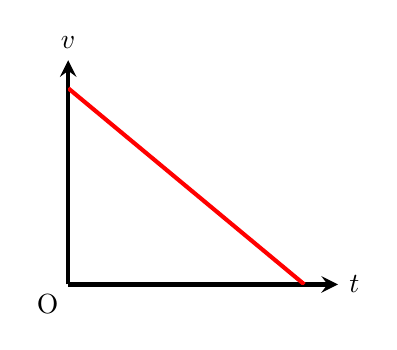
\begin{tikzpicture}  
		\begin{axis}[  ultra thick,scale=0.5,
			xmin=0,  
			xmax=4,  
			ymin=0,  
			ymax=4, 
			samples=300,
			yticklabels=\empty,
			xticklabels=\empty,
			xtick=\empty,
			ytick=\empty,
			axis lines=center, 
			xlabel=$t$, 		ylabel=$v$,
			every axis y label/.style={at=(current axis.above origin),anchor=south},  
			every axis x label/.style={at=(current axis.right of origin),anchor=west},  ]
			\addplot [line width=1.5pt, red, smooth, domain=0:3.5] {3.5-x};  
			\coordinate (O) at (0,0);
		\end{axis}  
		\node[below left] at (O) {O};
		\end{tikzpicture}&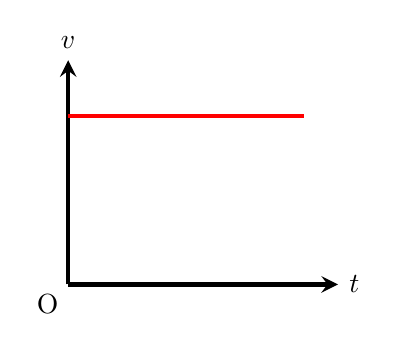
\begin{tikzpicture}  
		\begin{axis}[  ultra thick,scale=0.5,
			xmin=0,  
			xmax=4,  
			ymin=0,  
			ymax=4, 
			samples=300,
			yticklabels=\empty,
			xticklabels=\empty,
			xtick=\empty,
			ytick=\empty,
			axis lines=center, 
			xlabel=$t$, 		ylabel=$v$,
			every axis y label/.style={at=(current axis.above origin),anchor=south},  
			every axis x label/.style={at=(current axis.right of origin),anchor=west},  ]
			\addplot [line width=1.5pt, red, smooth, domain=0:3.5] {3};  
			\coordinate (O) at (0,0);
		\end{axis}  
		\node[below left] at (O) {O};
		\end{tikzpicture}\\
		Hình 1&Hình 2&Hình 3&Hình 4
	\end{tabular}
\end{center}	
	\choice
	{Hình 1 và Hình 4}
	{Hình 2 và Hình 3}
	{\True Hình 3}
	{Hình 1}
	\loigiai{}
\end{ex}
% ===================================================================
\begin{ex}
	Chọn phát biểu \textbf{sai}.
	\choice
	{Gia tốc của vật chuyển động thẳng biến đổi đều có độ lớn không đổi}
	{\True Trong chuyển động thẳng biến đổi đều, quãng đường vật đi được trong những khoảng thời gian bằng nhau thì bằng nhau}
	{Vận tốc tức thời của vật chuyển động thẳng biến đổi đều có độ lớn tăng hoặc giảm đều theo thời gian}
	{Vectơ gia tốc của vật chuyển động thẳng biến đổi đều có thể cùng chiều hoặc ngược chiều với vectơ vận tốc}
	\loigiai{}
\end{ex}
% ===================================================================
\begin{ex}
	Một ô tô đang chạy với tốc độ $\SI{72}{\kilo\meter/\hour}$ thì hãm phanh, chạy chậm dần đều sau $\SI{10}{\second}$ tốc độ giảm còn $\SI{10}{\meter/\second}$. Thời gian từ lúc hãm phanh đến lúc dừng lại là
	\choice
	{$\SI{30}{\second}$}
	{\True $\SI{20}{\second}$}
	{$\SI{12}{\second}$}
	{$\SI{40}{\second}$}
	\loigiai{}
\end{ex}
% ===================================================================
\begin{ex}
Trong chuyển động thẳng nhanh dần đều	
	\choice
	{$a<0$}
	{\True $v\cdot a>0$}
	{$ a>0$}
	{$v\cdot a<0$}
	\loigiai{}
\end{ex}
% ===================================================================
\begin{ex}
Một ô tô đang chạy với tốc độ $\SI{12}{\meter/\second}$ trên một đoạn đường thẳng thì người lái xe tăng
ga cho ôtô chạy nhanh dần đều. Sau $\SI{15}{\second}$ ôtô đạt tốc độ $\SI{15}{\meter/\second}$. Quãng đường của ô tô
đi được sau $\SI{5}{\second}$ kể từ khi tăng ga là	
	\choice
	{$\SI{72.5}{\meter}$}
	{$\SI{65}{\meter}$}
	{$\SI{57.5}{\meter}$}
	{\True $\SI{62.5}{\meter}$}
	\loigiai{}
\end{ex}
% ===================================================================
\begin{ex}
	Một đoàn tàu đang đứng yên  thì bắt đầu tăng tốc chuyển động thẳng nhanh dần đều. Trong khoảng thời gian tăng tốc từ $\SI{21.6}{\kilo\meter/\hour}$ đến $\SI{36}{\kilo\meter/\hour}$, tàu đi được $\SI{64}{\meter}$. Gia tốc của tàu và quãng đường tàu đi được kể từ lúc bắt đầu chuyển động đến khi đạt tốc độ $\SI{36}{\kilo\meter/\hour}$ là
	\choice
	{$a=\SI{-0.7}{\meter/\second^2}$, $s=\SI{200}{\meter}$}
	{$a=\SI{-0.5}{\meter/\second^2}$, $s=\SI{110}{\meter}$}
	{\True $a=\SI{0.5}{\meter/\second^2}$, $s=\SI{100}{\meter}$}
	{$a=\SI{-0.5}{\meter/\second^2}$, $s=\SI{100}{\meter}$}
	\loigiai{}
\end{ex}

% ===================================================================
\begin{ex}
Hình bên mô tả đồ thị $\left(v-t\right)$ của bốn xe ô tô A, B, C, D. Nhận định nào sau đây là đúng?
\begin{center}
	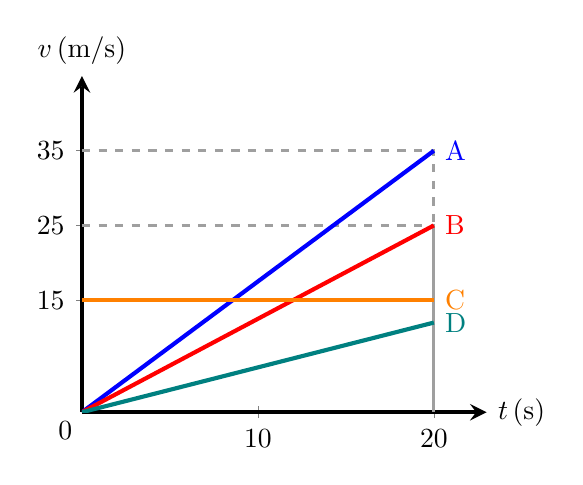
\begin{tikzpicture}  
		\begin{axis}[  ultra thick,scale=0.75,
			xmin=0,  
			xmax=23,  
			xtick={0,10,20},
			ytick={0,15,25,35},
			ymin=0,  
			ymax=45, 
			samples=300,
			axis lines=center, 
			xlabel=$\xsi{t}{\left(\si{\second}\right)}$, 		ylabel=$\xsi{v}{\left(\si{\meter/\second}\right)}$,
			every axis y label/.style={at=(current axis.above origin),anchor=south},  
			every axis x label/.style={at=(current axis.right of origin),anchor=west},  ]
			\draw[dashed, line width=1pt, gray!75!white] (axis cs: 0,35)--(axis cs: 20,35)--(axis cs: 20,0);
			\draw[dashed, line width=1pt, gray!75!white] (axis cs: 0,25)--(axis cs: 20,25)--(axis cs: 20,0);
			\addplot [line width=1.5pt, blue, smooth, domain=0:20] {1.75*x} node[right] {A};
			\addplot [line width=1.5pt, red, smooth, domain=0:20] {1.25*x} node[right] {B}; 
			\addplot [line width=1.5pt,teal , smooth, domain=0:20] {0.6*x} node[right] {D}; 
			\addplot [line width=1.5pt, orange, smooth, domain=0:20] {15} node[right] {C};
			\coordinate (O) at (0,0);
		\end{axis}  
		\node[below left] at (O) {0};
	\end{tikzpicture}
\end{center}	
	\choice
	{\True Xe C chuyển động đều, còn các xe còn lại là chuyển động biến đổi đều}
	{Chỉ có xe A và B chuyển động biến đồi đều, xe C chuyển động đều}
	{Gia tốc xe A có độ lớn nhỏ hơn gia tốc xe D}
	{Xe D chuyển động biến đổi đều, xe C chuyển động đều}
	\loigiai{}
\end{ex}
% ===================================================================
\begin{ex}
	Một vật chuyển động dọc theo trục $Ox$ có phương trình chuyển động $x=3-4t+2t^2\ \left(\si{\meter};\si{\second}\right)$. Biểu thức vận tốc của vật theo thời gian là
	\choice
	{$v=\xsi{2\left(t-2\right)}{\meter/\second}$}
	{$v=\xsi{2\left(t+2\right)}{\meter/\second}$}
	{\True $v=\xsi{4\left(t-1\right)}{\meter/\second}$}
	{$v=\xsi{2\left(t-1\right)}{\meter/\second}$}
	\loigiai{}
\end{ex}
% ===================================================================
\begin{ex}
Một vật chuyển động dọc theo trục $Ox$ có phương trình chuyển động $x=10t+5t^2\ \left(\si{\meter}; \si{\second}\right)$. Vận tốc của vật tại thời điểm $t=\SI{2}{\second}$ là	
	\choice
	{$\SI{40}{\meter/\second}$}
	{$\SI{20}{\meter/\second}$}
	{\True $\SI{30}{\meter/\second}$}
	{$\SI{26}{\meter/\second}$}
	\loigiai{}
\end{ex}
% ===================================================================
\begin{ex}
Phương trình chuyển động của một vật trên trục $Ox$ có dạng: $x=-2t^2+15t+10$.	Trong đó $t$ tính bằng giây, $x$ tính bằng mét. Vật này chuyển động
	\choice
	{nhanh dần đều rồi chậm dần đều theo chiều dương của trục $Ox$}
	{chậm dần đều rồi nhanh dần đều theo chiều âm của trục $Ox$}
	{nhanh dần đều rồi chậm dần đều theo chiều âm của trục $Ox$}
	{\True chậm dần đều theo chiều dương rồi nhanh dần đều theo chiều âm của trục $Ox$}
	\loigiai{}
\end{ex}
% ===================================================================
\begin{ex}
	\immini{Đồ thị vận tốc - thời gian của một vật chuyển động thẳng biến đổi trong 5 giây đầu tiên được cho như hình vẽ bên. Kết luận nào sau đây là đúng?
	\choice
	{\True Vật chuyển động chậm dần đều theo chiều âm với gia tốc $\SI{2}{\meter/\second^2}$}
	{Vật chuyển động thẳng đều theo chiều dương}
	{Vật chuyển động nhanh dần đều theo chiều dương với gia tốc $\SI{2}{\meter/\second^2}$}
	{Vật chuyển động nhanh dần đều theo chiều âm với gia tốc $\SI{-2}{\meter/\second^2}$}
	\loigiai{}}
	{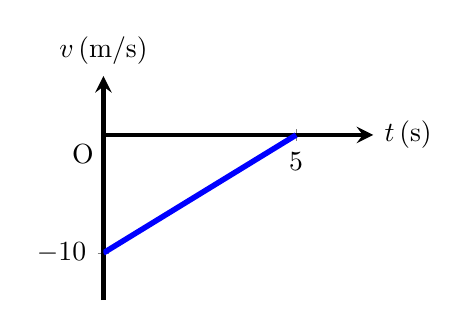
\begin{tikzpicture}  
			\begin{axis}[  ultra thick,scale=0.5,
				xmin=0,  
				xmax=7,  
				xtick={0,5},
				ytick={-10,0},
				ymin=-14,  
				ymax=5, 
				samples=300,
				axis lines=center, 
				xlabel=$\xsi{t}{\left(\si{\second}\right)}$, 		ylabel=$\xsi{v}{\left(\si{\meter/\second}\right)}$,
				every axis y label/.style={at=(current axis.above origin),anchor=south},  
				every axis x label/.style={at=(current axis.right of origin),anchor=west},  ]
				\addplot [line width=2pt, blue, smooth, domain=0:5] {-10+2*x};  
				\coordinate (O) at (axis cs: 0,0);
			\end{axis}  
			\node[below left] at (O) {O};
	\end{tikzpicture}}
\end{ex}
% ===================================================================
\begin{ex}
	Một vật chuyển động thẳng có đồ thị vận tốc theo thời gian như hình vẽ. Quãng đường vật đi được trong giai đoạn chậm dần đều là
	\begin{center}
		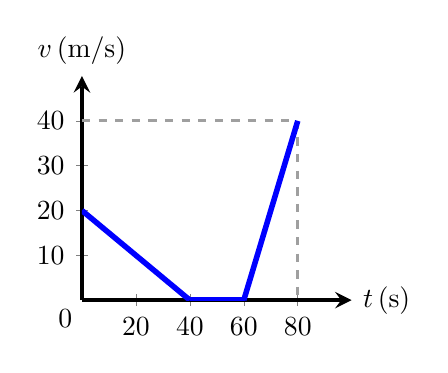
\begin{tikzpicture}  
			\begin{axis}[  ultra thick,scale=0.5,
				xmin=0,  
				xmax=100,  
				xtick={0,20,...,80},
				ytick={0,10,...,40},
				minor x tick num=0,
				minor y tick num=0,
				ymin=0,  
				ymax=50, 
				samples=300,
				axis lines=center, 
				xlabel=$\xsi{t}{\left(\si{\second}\right)}$, 		ylabel=$\xsi{v}{\left(\si{\meter/\second}\right)}$,
				every axis y label/.style={at=(current axis.above origin),anchor=south},  
				every axis x label/.style={at=(current axis.right of origin),anchor=west},  ]
				\draw[dashed, line width=1pt, gray!75!white] (axis cs: 0,40)--(axis cs: 80,40)--(axis cs: 80,0);
				\addplot [line width=2pt, blue, smooth, domain=0:40] {20-0.5*x};  
				\addplot [line width=2pt, blue, smooth, domain=40:60] {0}; 
				\addplot [line width=2pt, blue, smooth, domain=60:80] {2*(x-60)}; 
				\coordinate (O) at (0,0);
			\end{axis}  
			\node[below left] at (O) {0};
		\end{tikzpicture}
	\end{center}
	\choice
	{$\SI{600}{\meter}$}
	{$\SI{800}{\meter}$}
	{$\SI{200}{\meter}$}
	{\True $\SI{400}{\meter}$}
	\loigiai{}
\end{ex}
% ===================================================================
\begin{ex}
	Quan sát đồ thị $\left(v-t\right)$ như hình bên dưới của một vật đang chuyển động thẳng và cho biết quãng đường vật đi được trong khoảng thời gian nào lớn nhất?
	\begin{center}
		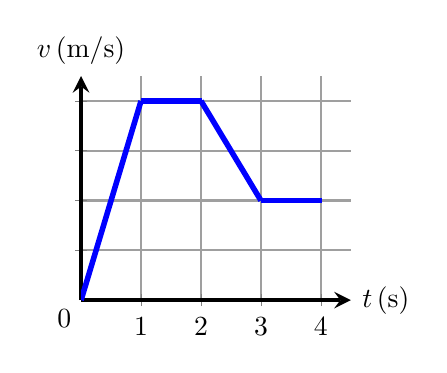
\begin{tikzpicture}  
			\begin{axis}[  ultra thick,scale=0.5,
				xmin=0,  
				xmax=4.5,  
				xtick={0,1,...,4},
				ytick={0,1,...,4},
				minor x tick num=0,
				minor y tick num=0,
				ymin=0,  
				ymax=4.5, 
				samples=300,
				yticklabels=\empty,
				axis lines=center, 
				grid style={step=1, line width =0.4pt, color=gray!40!white},
				grid=both, %giới hạn ô lưới
				major grid style={line width=0.8pt,gray!75!white},
				xlabel=$\xsi{t}{\left(\si{\second}\right)}$, 		ylabel=$\xsi{v}{\left(\si{\meter/\second}\right)}$,
				every axis y label/.style={at=(current axis.above origin),anchor=south},  
				every axis x label/.style={at=(current axis.right of origin),anchor=west},  ]
				\addplot [line width=2pt, blue, smooth, domain=0:1] {4*x};  
				\addplot [line width=2pt, blue, smooth, domain=1:2] {4}; 
				\addplot [line width=2pt, blue, smooth, domain=2:3] {4-2*(x-2)}; 
				\addplot [line width=2pt, blue, smooth, domain=3:4] {2}; 
				\coordinate (O) at (0,0);
			\end{axis}  
			\node[below left] at (O) {0};
		\end{tikzpicture}
	\end{center}
	\choice
	{Trong khoảng thời gian từ $\SI{0}{\second}$ đến $\SI{1}{\second}$}
	{\True Trong khoảng thời gian từ $\SI{1}{\second}$ đến $\SI{2}{\second}$}
	{Trong khoảng thời gian từ $\SI{2}{\second}$ đến $\SI{3}{\second}$}
	{Trong khoảng thời gian từ $\SI{3}{\second}$ đến $\SI{4}{\second}$}
	\loigiai{}
\end{ex}
% ===================================================================
\begin{ex}
Đồ thị vận tốc - thời gian của một vật chuyển động thẳng biến đổi đều được cho như hình vẽ bên. Biết rằng $v_1+v_2=\SI{15}{\meter/\second}$ và $t_2-t_1=\SI{6}{\second}$. Quãng đường vật đi được trong khoảng thời gian từ $t_1$ đến $t_2$ là
\begin{center}
	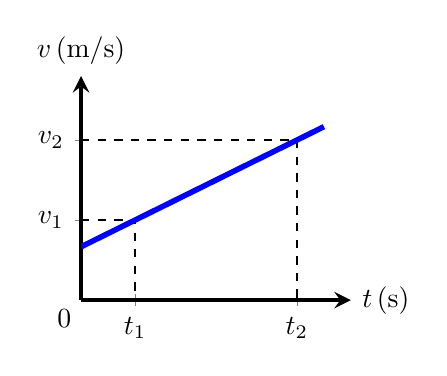
\begin{tikzpicture}  
		\begin{axis}[  ultra thick,scale=0.5,
			xmin=0,  
			xmax=10,  
			xtick={0,2,8},
			ytick={0,5,10},
			ymin=0,  
			ymax=14, 
			samples=300,
			yticklabels={0,$v_1$,$v_2$},
			xticklabels={0,$t_1$,$t_2$},
			axis lines=center, 
			xlabel=$\xsi{t}{\left(\si{\second}\right)}$, 		ylabel=$\xsi{v}{\left(\si{\meter/\second}\right)}$,
			every axis y label/.style={at=(current axis.above origin),anchor=south},  
			every axis x label/.style={at=(current axis.right of origin),anchor=west},  ]
			\draw[dashed, line width=1pt] (axis cs: 0,5)--(axis cs: 2,5)--(axis cs: 2,0);
			\draw[dashed, line width=1pt] (axis cs: 0,10)--(axis cs: 8,10)--(axis cs: 8,0);
			\addplot [line width=2pt, blue, smooth, domain=0:9] {10/3+5*x/6};  
			\coordinate (O) at (0,0);
		\end{axis}  
		\node[below left] at (O) {0};
	\end{tikzpicture}
\end{center}	
	\choice
	{$\SI{90}{\meter}$}
	{\True $\SI{45}{\meter}$}
	{$\SI{9}{\meter}$}
	{$\SI{540}{\meter}$}
	\loigiai{}
\end{ex}
% ===================================================================
\begin{ex}
	Một xe máy chạy đều trên một con đường thẳng với tốc độ $\SI{20}{\meter/\second}$ (vượt quá tốc độ) thì bị cảnh sát giao thông phát hiện. Chỉ sau $\SI{2}{\second}$ khi xe máy đi qua một cảnh sát, anh cảnh sát này bắt đầu đuổi theo với gia tốc không đổi và bằng $\SI{1.05}{\meter/\second^2}$. Thời điểm và vị trí anh cảnh sát đuổi kịp xe máy là
	\choice
	{\True sau $\SI{40}{\second}$ kể từ lúc anh cảnh sát xuất phát, cách vị trí xuất phát $\SI{840}{\meter}$}
	{sau $\SI{42}{\second}$ kể từ lúc anh cảnh sát xuất phát, cách vị trí xuất phát $\SI{840}{\meter}$}
	{sau $\SI{38}{\second}$ kể từ lúc anh cảnh sát xuất phát, cách vị trí xuất phát $\SI{760}{\meter}$}
	{sau $\SI{36}{\second}$ kể từ lúc anh cảnh sát xuất phát, cách vị trí xuất phát $\SI{760}{\meter}$}
	\loigiai{}
\end{ex}
% ===================================================================
\begin{ex}
	Hai xe A và B chuyển động cùng nhau vào hầm Thủ Thiêm dài $\SI{1490}{\meter}$. Xe A chuyển động với tốc độ ban đầu trước khi vào hầm là $\SI{60}{\kilo\meter/\hour}$ và chuyển động chậm dần đều với độ lớn gia tốc $\SI{144}{\kilo\meter/\hour^2}$, xe B chuyển động chậm dần đều với gia tốc $\SI{120}{\kilo\meter/\hour^2}$	từ lúc bắt đầu chạy vào hầm với tốc độ $\SI{55}{\kilo\meter/\hour}$. Nhận định nào sau đây là đúng về thời gian chuyển động của hai xe trong hầm?
	\choice
	{Hai xe đi hết hầm Thủ Thiêm cùng một khoảng thời gian}
	{Xe B ra khỏi hầm trước xe A}
	{\True Xe A ra khỏi hầm trước xe B}
	{Dữ liệu bài toán không đủ kết luận}
	\loigiai{}
\end{ex}
\Closesolutionfile{ans}
\section{TỰ LUẬN}
\Opensolutionfile{ans}[ans/BAI7-TL]
\setcounter{ex}{0}
% ======================================================================
\begin{ex}
	Quan sát đồ thị $\left(v-t\right)$ mô tả chuyển động thẳng của tàu hỏa trong hình bên dưới và trả lời các câu hỏi:
	\begin{center}
		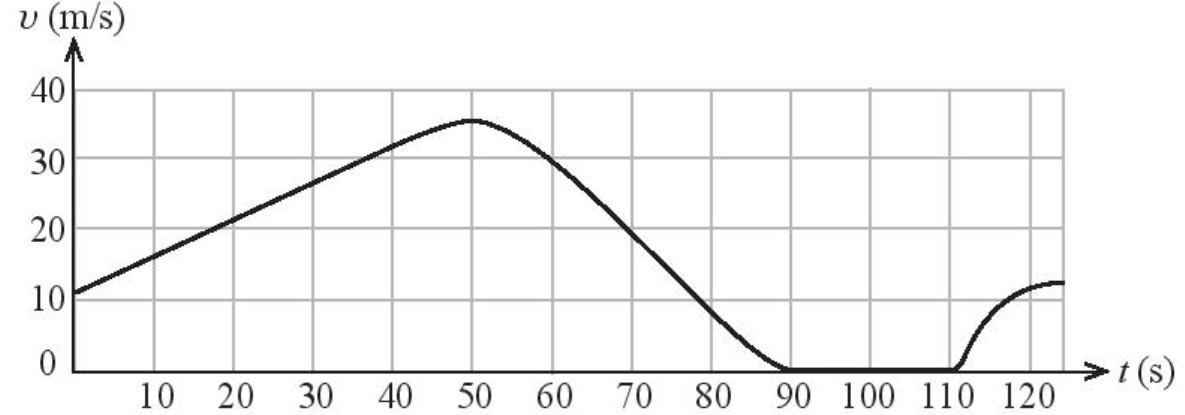
\includegraphics[width=0.65\linewidth]{figs/BAI7-1}
	\end{center}
	\begin{enumerate}[label=\alph*)]
		\item Tại thời điểm nào, vận tôc tàu hỏa có giá trị lớn nhất?
		\item Vận tốc tàu hỏa không đổi trong khoảng thời gian nào?
		\item Tàu chuyển động thẳng nhanh dần đều trong khoảng thời gian nào?
	\end{enumerate}
	\loigiai{}
\end{ex}

% ======================================================================
\begin{ex}
	Đồ thị vận tốc $(v)$ – thời gian $(t)$ của một vật chuyển động thẳng được cho như hình bên. Xác định quãng đường vật đi được trong 6 giây đầu tiên và 6 giây cuối cùng của chuyển động.
	\begin{center}
		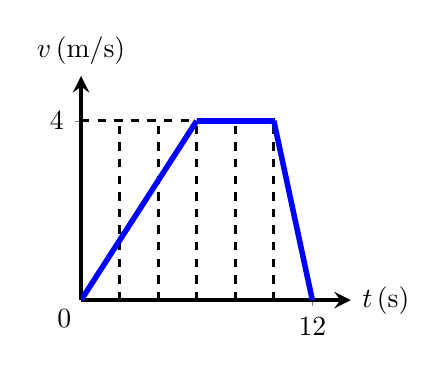
\begin{tikzpicture}  
			\begin{axis}[  ultra thick,scale=0.5,
				xmin=0,  
				xmax=14,  
				xtick={0,12},
				ytick={0,4},
				ymin=0,  
				ymax=5, 
				samples=300,
				axis lines=center,
				xlabel=$\xsi{t}{\left(\si{\second}\right)}$, 		ylabel=$\xsi{v}{\left(\si{\meter/\second}\right)}$,
				every axis y label/.style={at=(current axis.above origin),anchor=south},  
				every axis x label/.style={at=(current axis.right of origin),anchor=west},  ]
				\foreach \i in {2,4,...,10}{
				\edef\temp{\noexpand\draw[dashed, line width=1pt] (axis cs: \i,0)--(axis cs: \i,4);}
				\temp
				}
				\draw[dashed, line width=1pt] (axis cs: 0,4)--(axis cs: 10,4);
				\draw[dashed, line width=1pt] (axis cs: 0,40)--(axis cs: 80,40)--(axis cs: 80,0);
				\addplot [line width=2pt, blue, smooth, domain=0:6] {2*x/3};  
				\addplot [line width=2pt, blue, smooth, domain=6:10] {4}; 
				\addplot [line width=2pt, blue, smooth, domain=10:12] {4-2*(x-10)}; 
				\coordinate (O) at (0,0);
			\end{axis}  
			\node[below left] at (O) {0};
		\end{tikzpicture}
	\end{center}
	\loigiai{}
\end{ex}
% ======================================================================
\begin{ex}
	Một người đạp xe trên đường thẳng với tốc độ $\SI{4}{\meter/\second}$, bóp thắng để giảm tốc với gia tốc có độ lớn không đổi là $\SI{0.5}{\meter/\second^2}$. Xác định thời gian và quãng đường xe đi được từ khi bóp thắng đến khi dừng lại.
	\loigiai{}
\end{ex}
% ======================================================================
\begin{ex}
	Một ô tô chuyễn động chầm dần đều, trong $\SI{8.5}{\second}$ đi được quãng đường $\SI{40.0}{\meter}$ với vận tốc cuối cùng là $\SI{2.80}{\meter/\second}$.
	\begin{enumerate}[label=\alph*)]
		\item Tìm độ lớn vận tốc ban đầu của xe.
		\item Tìm gia tốc của xe.
	\end{enumerate}
	\loigiai{}
\end{ex}
% ======================================================================
\begin{ex}
Tại hiện trường một vụ tai nạn trên đường quốc lộ ngoài đô thị, cảnh sát phát hiện vết trượt kéo dài $\SI{50}{\meter}$. Qua các đo đạc trên mặt đường, cảnh sát kết luận gia tốc của ô tô trong quá trình giảm tốc có độ lớn $\SI{6.5}{\meter/\second^2}$. Nếu tốc độ giới hạn trên làn đường được quy định là $\SI{80}{\kilo\meter/\hour}$ thì ô tô này có vượt quá tốc độ cho phép không? Giả sử trong quá trình giảm tốc, ô tô chuyển động chậm dần đều.
	\loigiai{}
\end{ex}
% ======================================================================
\begin{ex}
	Một ô tô đang đi trên đường thẳng với tốc độ $v$ thì trước mặt ô tô đột ngột xuất hiện một mối nguy hiểm. Trong khoảng thời gian từ khi mối nguy xuất hiện đến khi phanh hoạt động, ô tô chuyển động được quãng đường $\SI{29.3}{\meter}$. Khi phanh hoạt động làm bánh xe ngừng quay, các bánh xe của ô tô để lại vết trượt dài $\SI{12.8}{\meter}$ trên đường, như minh hoạ trong hình bên dưới.
	\begin{center}
		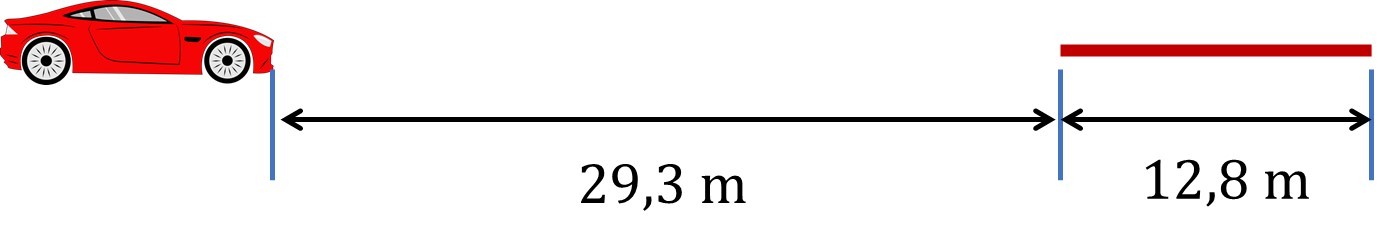
\includegraphics[width=0.5\linewidth]{figs/BAI7-2}
	\end{center}
	Người ta ước tính rằng trong quá trình trượt, ô tô giảm tốc với gia tốc có độ lớn là $\SI{8.33}{\meter/\second^2}$. Xác định:
	\begin{enumerate}[label=\alph*)]
		\item Tốc độ $v$ của ô tô trước khi hãm phanh.
		\item Khoảng thời gian từ khi nguy hiểm xuất hiện đến khi phanh hoạt động.
	\end{enumerate}
	\loigiai{}
\end{ex}
% ======================================================================
\begin{ex}
	Một ô tô khi hãm phanh có thể có gia tốc $\SI{3}{\meter/\second^2}$. Hỏi khi ô tô đang chạy với vận tốc là $\SI{72}{\kilo\meter/\hour}$ thì phải hãm phanh cách vật cản là bao nhiêu mét để không đâm vào vật cản? Thời gian hãm phanh là bao nhiêu?
	\loigiai{}
\end{ex}
% ======================================================================
\begin{ex}
	Một xe đạp đang đi với tốc độ $\SI{2}{\meter/\second}$ thì xuống dốc chuyển động nhanh dần đều với độ lớn gia tốc $\SI{0.2}{\meter/\second^2}$. Cùng lúc đó, một ô tô đang chạy với tốc độ $\SI{20}{\meter/\second}$ lên dốc,
	chuyển động chậm dần đều với độ lớn gia tốc $\SI{0.4}{\meter/\second^2}$. Xác định vị trí hai xe gặp nhau trên dốc. Biết dốc dài $\SI{570}{\meter}$.
	\loigiai{$\SI{420}{\meter}$}
\end{ex}
% ======================================================================
\begin{ex}
	\immini{
	Hai vật A và B chuyển động cùng chiều trên đường thẳng (theo hướng từ A sang B) có đồ thị vận tốc - thời gian vẽ ở hình vẽ bên. Biết ban đầu hai vật cách nhau $\SI{78}{\meter}$.
	\begin{enumerate}[label=\alph*)]
		\item Hai vật có cùng vận tốc ở thời điểm nào?
		\item Viết phương trình chuyển động của mỗi vật.
		\item Xác định vị trí gặp nhau của hai vật.
	\end{enumerate}
	}
	{
	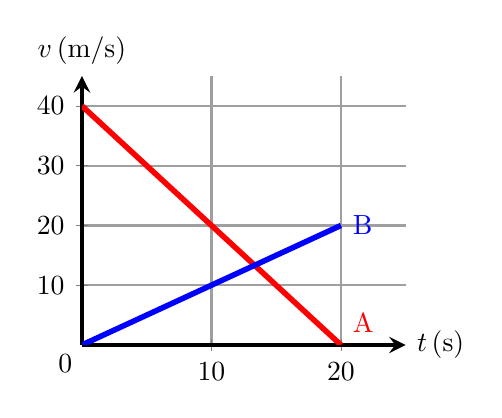
\begin{tikzpicture}  
		\begin{axis}[  ultra thick,scale=0.6,
			xmin=0,  
			xmax=25,  
			xtick={0,10,20},
			ytick={0,10,...,40},
			minor x tick num=0,
			minor y tick num=0,
			ymin=0,  
			ymax=45, 
			samples=300,
			axis lines=center, 
			grid style={step=1, line width =0.4pt, color=gray!40!white},
			grid=both, %giới hạn ô lưới
			major grid style={line width=0.8pt,gray!75!white},
			xlabel=$\xsi{t}{\left(\si{\second}\right)}$, 		ylabel=$\xsi{v}{\left(\si{\meter/\second}\right)}$,
			every axis y label/.style={at=(current axis.above origin),anchor=south},  
			every axis x label/.style={at=(current axis.right of origin),anchor=west},  ]
			\addplot [line width=2pt, red, smooth, domain=0:20] {40-2*x} node[above right] {A}; 
			\addplot [line width=2pt, blue, smooth, domain=0:20] {x} node[right] {B};  
			\coordinate (O) at (axis cs: 0,0);
		\end{axis}  
		\node[below left] at (O) {0};
	\end{tikzpicture}
	}
	\loigiai{}
\end{ex}
% ======================================================================
\begin{ex}
	Một người đứng ở sân ga nhìn ngang đầu toa tàu thứ nhất của một đoàn tàu bắt đầu chuyển bánh. Thời gian toa thứ nhất qua trước mặt người ấy là $t_1=\SI{6}{\second}$. Hỏi toa thứ 7 qua trước mặt người ấy trong bao lâu? Biết rằng đoàn tàu chuyển động thẳng nhanh dần đều, chiều dài các toa bằng nhau và khoảng hở giữa 2 toa là không đáng kể.
	\loigiai{}
\end{ex}
\Closesolutionfile{ans}
\begin{center}
	\textbf{-- HẾT --}
\end{center}
%	% ======================================================================
\begin{ex}
	Một xe chuyển động thẳng nhanh dần đều đi trên hai đoạn đường liên tiếp bằng nhau $\SI{100}{\meter}$, lần lượt trong $\SI{5}{\second}$ và $\SI{3}{\second}$. Tính gia tốc của xe.
	\loigiai{}
\end{ex}
% ======================================================================
\begin{ex}
	Hai người đi xe đạp khởi hành cùng lúc và đi ngược chiều. Người thứ nhất có vận tốc đầu là $\SI{4.5}{\kilo\meter/\hour}$ và nhanh dần đều với gia tốc $\SI{20}{\centi\meter/\second^2}$. Người thứ hai có vận tốc đầu $\SI{5.4}{\kilo\meter/\hour}$ và đi nhanh dần đều với với gia tốc $\SI{0.2}{\meter/\second^2}$. Khoảng cách ban đầu là $\SI{130}{\meter}$. Xác định thời điểm để hai xe cách nhau $\SI{40}{\meter}$?
	
	\loigiai{}
\end{ex}
% ======================================================================
\begin{ex}
	Một ôtô chuyển động trên đường thẳng, bắt đầu khởi hành nhanh dần đều với gia tốc $a_1=\SI{5}{\meter/\second^2}$, sau đó chuyển động thẳng đều và cuối cùng chuyển động chậm dần đều với gia tốc $a_3 = \SI{5}{\meter/\second^2}$ cho đến khi dừng lại. Thời gian ôtô chuyển động là $\SI{25}{\second}$. Tốc độ trung bình của ô tô trên cả đoạn đường là $\SI{20}{\meter/\second}$. Trong giai đoạn chuyển động thẳng đều ôtô đạt vận tốc là bao nhiêu?
	\loigiai{}
\end{ex}
%	\begin{center}\textbf{\color{red}LUYỆN TẬP}\\
\textbf{CHUYỂN ĐỘNG THẲNG ĐỀU - CHUYỂN ĐỘNG TỔNG HỢP\\ GIA TỐC - CHUYỂN ĐỘNG THẲNG BIẾN ĐỔI ĐỀU}
\end{center}
\setcounter{ex}{0}
\Opensolutionfile{ans}[ans/BAITAPTHEMPTCD-TN]
% ===================================================================
\begin{ex}
	Một chiếc xe ô tô xuất phát từ A lúc 6 giờ sáng, chuyển động thẳng đều tới B, cách A $\SI{180}{\kilo\meter}$. Xe tới B lúc 8 giờ 30 phút. Sau 30 phút đỗ tại B, xe chạy ngược về A với tốc độ $\SI{60}{\kilo\meter/\hour}$. Ô tô về tới A lúc
	\choice
	{$\SI{10}{\hour}$}
	{\True $\SI{12}{\hour}$}
	{$\SI{11}{\hour}$}
	{$\SI{10.5}{\hour}$}
	\loigiai{}
\end{ex}
% ===================================================================
\begin{ex}
	Một thuyền đi từ bến A đến bến B rồi lại trở về A. Biết rằng vận tốc thuyền trong nước yên lặng là $\SI{5}{\kilo\meter/\hour}$, vận tốc nước chảy là $\SI{1}{\kilo\meter/\hour}$. Vận tốc của thuyền so với bờ khi đi xuôi dòng là	
	\choice
	{$\SI{4}{\kilo\meter/\hour}$}
	{$\SI{4}{\meter/\second}$}
	{\True $\SI{6}{\kilo\meter/\hour}$}
	{$\SI{6}{\meter/\second}$}
	\loigiai{}
\end{ex}

% ===================================================================
\begin{ex}
	Đồ thị vận tốc – thời gian của một vật chuyển động như hình vẽ. Tỉ số gia tốc của vật trong thời gian OA và AB là
	\begin{center}
		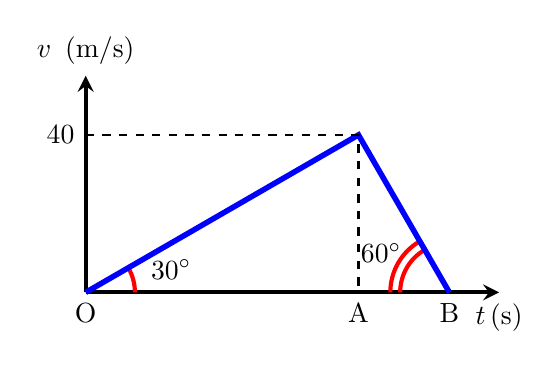
\begin{tikzpicture}[scale=0.5]
			\coordinate (O) at (0,0);
			\coordinate (D) at (0,4);
			\coordinate (A) at (6.9282,0);
			\coordinate (B) at (9.2376,0);
			\coordinate (C) at (6.9282,4);
			\coordinate (t) at (10.5,0);
				\coordinate (v) at (0,5.5);
				\draw[-stealth, line width=1.5pt] (O)--(t);
				\draw[-stealth, line width=1.5pt] (O)--(v);
				\tkzMarkAngle[size=1.25cm,color=red, line width=1.5pt](A,O,C);
				\tkzLabelAngle[color=black,pos=2.25](A,O,C){$\SI{30}{\degree}$};
				\tkzMarkAngle[size=1.25cm,color=red, line width=1.5pt](C,B,A);
				\tkzMarkAngle[size=1.5cm,color=red, line width=1.5pt](C,B,A);
				\tkzLabelAngle[color=black,pos=2](C,B,A){$\SI{60}{\degree}$}
				\draw[line width=2pt, blue] (O)--(C)--(B);
				\draw[line width=1pt,dashed] (D)--(C)--(A);
				\node[left] at (D) {$40$};
				\node[below] at (t) {$\xsi{t}{\left(\second\right)}$};
				\node[above] at (v) {$v\ \left(\si{\meter/\second}\right)$};
				\node[below] at (O) {O};
				\node[below] at (A) {A};
				\node[below] at (B) {B};
		\end{tikzpicture}
	\end{center}
	\choice
	{$\dfrac{1}{3}$}
	{\True $-\dfrac{1}{3}$}
	{$3$}
	{$-3$}
	\loigiai{}
\end{ex}

% ===================================================================
\begin{ex}
	Một chất điểm chuyển động với phương trình vận tốc $v = 8 - 2t$; với ($t$ tính bằng giây và $v$ tính bằng $\si{\meter/\second}$). Thời gian chất điểm dừng lại là
	\choice
	{\True $\SI{4}{\second}$}
	{$\SI{2}{\second}$}
	{$\SI{8}{\second}$}
	{$\SI{1}{\second}$}
	\loigiai{}
\end{ex}

% ===================================================================
\begin{ex}
	Một đoàn tàu đang chạy với tốc độ $\SI{72}{\kilo\meter/\hour}$, thì hãm phanh, sau $\SI{10}{\second}$ thì dừng hẳn. Sau thời gian 4 giây, kể từ lúc hãm phanh, đoàn tàu có tốc độ là
	\choice
	{$\SI{10}{\meter/\second}$}
	{$\SI{8}{\meter/\second}$}
	{$\SI{6}{\meter/\second}$}
	{\True $\SI{12}{\meter/\second}$}
	\loigiai{}
\end{ex}
% ===================================================================
\begin{ex}
	Một chất điểm chuyển động dọc theo trục $Ox$ có phương trình tọa độ $x=4-10t$ trong đó $x$ tính theo đơn vị $\si{\kilo\meter}$ và $t$ tính theo đơn vị giờ. Quãng đường đi được của chất điểm sau 2 giờ chuyển động là
	\choice
	{$\SI{8}{\kilo\meter}$}
	{$\SI{16}{\kilo\meter}$}
	{\True $\SI{20}{\kilo\meter}$}
	{$\SI{12}{\kilo\meter}$}
	\loigiai{}
\end{ex}
% ===================================================================
\begin{ex}
	Cho đồ thị tọa độ - thời gian của một chiếc xe chuyển động thẳng như hình bên dưới. 
	\begin{center}
		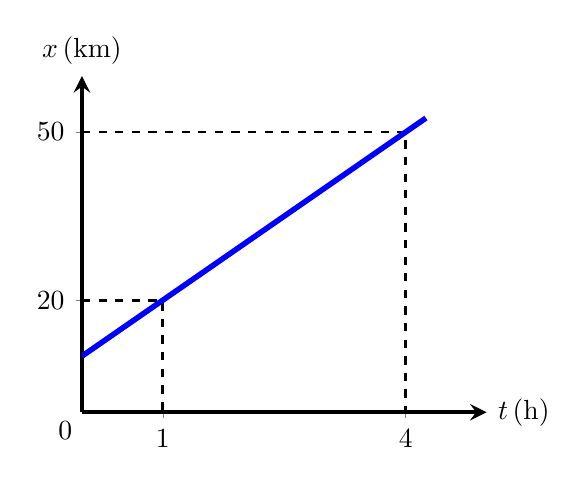
\begin{tikzpicture}  
			\begin{axis}[  ultra thick,scale=0.75,
				xmin=0,  
				xmax=5,  
				xtick={0,1,4},
				ytick={0,20,50},
				minor x tick num=0,
				minor y tick num=0,
				ymin=0,  
				ymax=60, 
				samples=300,
				axis lines=center, 
				xlabel=$\xsi{t}{\left(\si{\hour}\right)}$, 		ylabel=$\xsi{x}{\left(\si{\kilo\meter}\right)}$,
				every axis y label/.style={at=(current axis.above origin),anchor=south},  
				every axis x label/.style={at=(current axis.right of origin),anchor=west},  ]
				\draw[dashed, line width=1pt] (axis cs: 0,20)--(axis cs:1,20)--(axis cs:1,0);
				\draw[dashed, line width=1pt] (axis cs:0,50)--(axis cs:4,50)--(axis cs:4,0);
				\addplot [line width=2pt, blue, smooth, domain=0:4.25] {20+10*(x-1)};  
				\coordinate (O) at (axis cs: 0,0);
			\end{axis}  
			\node[below left] at (O) {0};
		\end{tikzpicture}
	\end{center}
	Phương trình tọa độ của xe là
	
	\choice
	{$x=15+5t$}
	{\True $x=10+10t$}
	{$x=20+10t$}
	{$x=-10+15t$}
	\loigiai{}
\end{ex}


% ===================================================================
\begin{ex}
	Một dòng sông có chiều rộng $\SI{60}{\meter}$, nước chảy với vận tốc $\SI{1}{\meter/\second}$ so với bờ. Một người lái đò chèo một chiếc thuyền đi trên sông với vận tốc $\SI{3}{\meter/\second}$ so với nước. Khi đi từ bờ này theo phương vuông góc sang bờ đối diện (điểm dự định đến). Do nước chảy nên khi sang đến bờ kia, thuyền bị trôi về phía cuối dòng. Khoảng cách từ điểm dự định đến và điểm thuyền đến thực cách nhau là
	\choice
	{$\SI{180}{\meter}$}
	{\True $\SI{20}{\meter}$}
	{$\SI{63}{\meter}$}
	{$\SI{18}{\meter}$}
	\loigiai{}
\end{ex}
% ===================================================================
\begin{ex}
Ở trên một đoạn dốc thẳng dài $\SI{130}{\meter}$, Tâm và Gia Huy đều đi xe đạp và khởi hành cùng một lúc ở hai đầu đoạn dốc. Tâm đi lên dốc với tốc độ $\SI{18}{\kilo\meter/\hour}$ và chuyển động chậm dần đều với gia tốc có độ lớn $\SI{0.2}{\meter/\second^2}$. Gia Huy đi xuống dốc với tốc độ $\SI{5.4}{\kilo\meter/\hour}$ và chuyển động nhanh dần đều với gia tốc có độ lớn $\SI{20}{\centi\meter/\second^2}$. Chọn chiều dương là chiều từ đỉnh đến chân dốc, gốc toạ độ tại đỉnh dốc, gốc thời gian là lúc hai bạn khởi hành. Phương trình chuyển động của Tâm và Gia Huy lần lượt là 
	\choice
	{$x_1=130+5t-0,1t^2\ \left(\si{\meter}, \si{\second}\right)$;  $x_2=1,5t-0,1t^2\ \left(\si{\meter}, \si{\second}\right)$}
	{$x_1=130-5t-0,1t^2\ \left(\si{\meter}, \si{\second}\right)$;  $x_2=1,5t-0,1t^2\ \left(\si{\meter}, \si{\second}\right)$}
	{$x_1=130-5t+0,1t^2\ \left(\si{\meter}, \si{\second}\right)$;  $x_2=-1,5t+0,1t^2\ \left(\si{\meter}, \si{\second}\right)$}
	{\True $x_1=130-5t+0,1t^2\ \left(\si{\meter}, \si{\second}\right)$;  $x_2=1,5t+0,1t^2\ \left(\si{\meter}, \si{\second}\right)$}
	\loigiai{}
\end{ex}

% ===================================================================
\begin{ex}
	Cùng một lúc ở hai địa điểm A, B cách nhau $\SI{300}{\meter}$, có hai xe đi ngược chiều nhau. Xe thứ nhất đi từ A với tốc độ ban đầu là $\SI{10}{\meter/\second}$ và chuyển động nhanh dần đều với gia tốc có độ lớn $\SI{2}{\meter/\second^2}$, còn xe thứ hai đi từ B với tốc độ ban đầu là $\SI{30}{\meter/\second}$ và chuyển động chậm dần đều với gia tốc có độ lớn $\SI{2}{\meter/\second^2}$. Chọn A làm gốc tọa độ, chiều dương hướng từ A đến B, gốc thời gian lúc xe thứ nhất đi qua A. Thời điểm và vị trí hai xe gặp nhau là
	\choice
	{\True $\SI{7.5}{\second}$ và $\SI{131.25}{\meter}$}
	{$\SI{10}{\second}$ và $\SI{131}{\meter}$}
	{$\SI{7.5}{\second}$ và $\SI{225}{\meter}$}
	{$\SI{15}{\second}$ và $\SI{150}{\meter}$}
	\loigiai{}
\end{ex}

\Closesolutionfile{ans}
\newpage
\begin{center}
	\textbf{BẢNG ĐÁP ÁN}
\end{center}
\inputansbox{10}{ans/BAITAPTHEMPTCD-TN}\newpage
%	\begin{center}\textbf{\color{red}LUYỆN TẬP}\\
	\textbf{CHUYỂN ĐỘNG THẲNG ĐỀU - CHUYỂN ĐỘNG TỔNG HỢP\\ GIA TỐC - CHUYỂN ĐỘNG THẲNG BIẾN ĐỔI ĐỀU}
\end{center}
\setcounter{ex}{0}
\Opensolutionfile{ans}[ans/BAITAPTHEMPTCD2-TN]

% ===================================================================
\begin{ex}
	An chạy bộ qua cầu vượt với vận tốc $\SI{3}{\meter/\second}$ theo hướng từ Nam đến Bắc. Đúng lúc đó Hùng chạy bộ dưới cầu vượt theo hướng từ Đông sang Tây với vận tốc $\SI{4}{\meter/\second}$. Vận tốc của An đối với Hùng là 
	\choice
	{$\SI{7}{\meter/\second}$}
	{$\SI{1}{\meter/\second}$}
	{\True $\SI{5}{\meter/\second}$}
	{$\SI{3.5}{\meter/\second}$}
	\loigiai{}
\end{ex}
% ===================================================================
\begin{ex}
	Một xe chuyển động thẳng không đổi chiều có tốc độ trung bình là $\SI{20}{\kilo\meter/\hour}$ trên  $\frac{1}{4}$ đoạn đường đầu và $\SI{40}{\kilo\meter/\hour}$ trên $\frac{3}{4}$ đoạn đường còn lại. Tốc độ trung bình của xe trên cả đoạn đường là 	
	\choice
	{$\SI{30}{\kilo\meter/\hour}$}
	{\True $\SI{32}{\kilo\meter/\hour}$}
	{$\SI{26.67}{\kilo\meter/\hour}$}
	{$\SI{35}{\kilo\meter/\hour}$}
	\loigiai{}
\end{ex}
% ===================================================================
\begin{ex}
	Khi đang chạy với tốc độ $\SI{36}{\kilo\meter/\hour}$ thì ô tô bắt đầu chạy xuống dốc. Nhưng do bị mất phanh nên ô tô chuyển động nhanh dần đều với gia tốc $\SI{0.2}{\meter/\second^2}$ xuống hết đoạn dốc có độ dài $\SI{960}{\meter}$. Thời gian ô tô chạy xuống hết đoạn dốc là 
	\choice
	{$\SI{90}{\second}$}
	{\True $\SI{60}{\second}$}
	{$\SI{160}{\second}$}
	{$\SI{20}{\second}$}
	\loigiai{}
\end{ex}
% ===================================================================
\begin{ex}
	Đồ thị độ dịch chuyển – thời gian của một vật chuyển động như hình vẽ. Vật chuyển động
	\begin{center}
		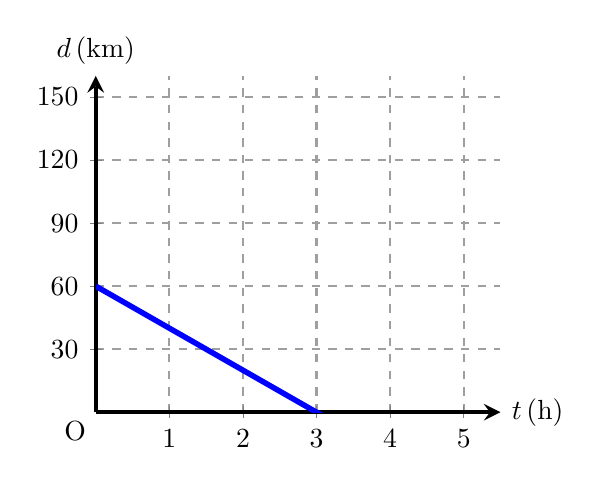
\begin{tikzpicture}  
			\begin{axis}[  ultra thick, scale=0.75,
				xmin=0,  
				xmax=5.5,  
				xtick={0,1,...,5},
				ytick={0,30,...,150},
				minor x tick num=0,
				minor y tick num=0,
				ymin=0,  
				ymax=160, 
				samples=300,
				axis lines=center, 
				grid style={step=1, line width =0.4pt, color=gray!40!white},
				grid=both, %giới hạn ô lưới
				major grid style={line width=0.8pt,gray!75!white, dashed},
				xlabel=$\xsi{t}{\left(\si{\hour}\right)}$, 		ylabel=$\xsi{d}{\left(\si{\kilo\meter}\right)}$,
				every axis y label/.style={at=(current axis.above origin),anchor=south},  
				every axis x label/.style={at=(current axis.right of origin),anchor=west},  ]
				\addplot [line width=2pt, blue, smooth, domain=0:5] {60-20*x};  
				\coordinate (O) at (axis cs: 0,0);
			\end{axis}  
			\node[below left] at (O) {O};
		\end{tikzpicture}
	\end{center}
	\choice
	{cùng chiều dương với tốc độ $\SI{60}{\kilo\meter/\hour}$}
	{\True ngược chiều dương với tốc độ $\SI{20}{\kilo\meter/\hour}$}
	{cùng chiều dương với tốc độ $\SI{20}{\kilo\meter/\hour}$}
	{ngược chiều dương với tốc độ $\SI{60}{\kilo\meter/\hour}$}
	\loigiai{}
\end{ex}
% ===================================================================
\begin{ex}
	Phương trình nào sau đây là phương trình tọa độ của một vật chuyển động thẳng chậm dần đều dọc theo trục $Ox$?
	\choice
	{$x=4-t$}
	{$x=6+t^2$}
	{$x=2-5t-t^2$}
	{\True $x=5t^2-2t+5$}
	\loigiai{}
\end{ex}

% ===================================================================
\begin{ex}
	Một vật chuyển động thẳng dọc theo trục $Ox$ có phương trình tọa độ: $x=4+20t+0,4t^2$ với $x$ tính bằng mét và $t$ tính bằng giây. Quãng đường vật đi được trong khoảng thời gian từ $t_1=\SI{1}{\second}$ đến $t_2=\SI{4}{\second}$ là
	\choice
	{$\SI{20.6}{\meter}$}
	{$\SI{26}{\meter}$}
	{\True $\SI{66}{\meter}$}
	{$\SI{67.6}{\meter}$}
	\loigiai{}
\end{ex}
% ===================================================================
\begin{ex}
	Đồ thị vận tốc - thời gian của một vật chuyển động được biểu diễn như hình vẽ. Quãng đường vật đi được từ thời điểm $t = 0$, đến thời điểm $t = \SI{60}{\second}$ là
	\begin{center}
		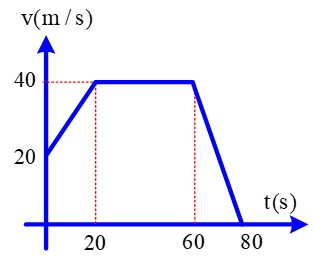
\includegraphics[width=0.3\linewidth]{figs/G10-BTTHEMPTCD-1}
	\end{center}
	\choice
	{\True $\SI{2.2}{\kilo\meter}$}
	{$\SI{1.1}{\kilo\meter}$}
	{$\SI{440}{\meter}$}
	{$\SI{1.2}{\kilo\meter}$}
	\loigiai{}
\end{ex}

% ===================================================================
\begin{ex}
	Hai xe máy cùng xuất phát từ hai địa điểm A và B cách nhau $\SI{400}{\meter}$ và cùng chạy theo hướng AB trên đoạn đường thẳng đi qua A và B. Xe máy xuất phát từ A chuyển động nhanh dần đều với gia tốc $\SI{2.5E-2}{\meter/\second^2}$. Xe máy xuất phát từ B chuyển động với gia tốc $\SI{2.0E-2}{\meter/\second^2}$. Tại vị trí hai xe đuổi kịp nhau thì tốc độ của xe xuất phát từ A và xe xuất phát từ B lần lượt là	
	\choice
	{$\SI{8}{\meter/\second}$; $\SI{10}{\meter/\second}$}
	{\True $\SI{10}{\meter/\second}$; $\SI{8}{\meter/\second}$}
	{$\SI{6}{\meter/\second}$; $\SI{4}{\meter/\second}$}
	{$\SI{4}{\meter/\second}$; $\SI{6}{\meter/\second}$}
	\loigiai{}
\end{ex}
% ===================================================================
\begin{ex}
	Lúc 8 giờ sáng một ôtô đi qua điểm A trên một đường thẳng với tốc độ $\SI{10}{\meter/\second}$, chuyển động chậm dần đều với độ lớn gia tốc $\SI{0.2}{\meter/\second^2}$. Cùng lúc đó tại điểm B cách A $\SI{390}{\meter}$, một ôtô thứ hai bắt đầu khởi hành đi ngược chiều với xe thứ nhất, chuyển động nhanh dần đều với độ lớn gia tốc $\SI{0.4}{\meter/\second^2}$. Hai xe gặp nhau ở vị trí cách A là 
	\choice
	{$\SI{240}{\meter}$}
	{\True $\SI{210}{\meter}$}
	{$\SI{250}{\meter}$}
	{$\SI{150}{\meter}$}
	\loigiai{}
\end{ex}
% ===================================================================
\begin{ex}
	Một xe máy chuyển động thẳng nhanh dần đều trên đoạn AD dài $\SI{28}{\meter}$. Sau khi xe qua A được $\SI{1}{\second}$ xe tới B với vận tốc $\SI{6}{\meter/\second}$. $\SI{1}{\second}$ trước khi tới D, xe ở C với vận tốc $\SI{8}{\meter/\second}$. Thời gian xe đi trên đoạn đường AD là
	\choice
	{$\SI{10}{\second}$}
	{$\SI{7}{\second}$}
	{$\SI{3}{\second}$}
	{\True $\SI{4}{\second}$}
	\loigiai{
	}
\end{ex}
\Closesolutionfile{ans}
\newpage
\begin{center}
	\textbf{BẢNG ĐÁP ÁN}
\end{center}
\inputansbox{10}{ans/BAITAPTHEMPTCD2-TN}
%	\begin{center}\textbf{\color{red}LUYỆN TẬP}\\
\textbf{CHUYỂN ĐỘNG NÉM}
\end{center}

%	\begin{center}\textbf{\color{red}LUYỆN TẬP}\\
	\textbf{CHUYỂN ĐỘNG NÉM}
\end{center}
\section{BÀI TẬP TRẮC NGHIỆM}
% ===================================================================
\begin{ex}
Một vật rơi có khối lượng $m$, được ném ngang với vận tốc ban đầu $v_0$ ở độ cao $h$. Bỏ qua sức cản của không khí. Thời gian rơi	
	\choice
	{chỉ phụ thuộc vào $m$}
	{\True chỉ phụ thuộc vào $h$}
	{phụ thuộc $v_0$ và $h$}
	{phụ thuộc vào $m$, $v_0$, $h$}
	\loigiai{}
\end{ex}
% ===================================================================
\begin{ex}
	Một vật có khối lượng $m$, được ném ngang với vận tốc ban đầu $v_0$ ở độ cao $h$. Bỏ qua sức cản của không khí. Tầm bay xa của vật phụ thuộc vào
	\choice
	{$m$ và $v_0$}
	{$m$ và $h$}
	{$v_0$ và $h$}
	{$m$, $v_0$ và $h$}
	\loigiai{}
\end{ex}
% ===================================================================
\begin{ex}
	Quỹ đạo chuyển động của vật ném ngang là một 
	\choice
	{đường thẳng}
	{đường tròn}
	{đường xoắn ốc}
	{nhánh parabol}
	\loigiai{}
\end{ex}
% ===================================================================
\begin{ex}
	Quả cầu I có khối lượng  gấp đôi quả cầu II. Cùng một lúc tại độ cao $h$, quả cầu I được thả rơi còn quả cầu II được ném theo phương ngang. Bỏ qua sức cản của không khí. Chọn phát biểu đúng?
	\choice
	{Quả cầu I chạm đất trước}
	{Quả cầu II chạm đất trước}
	{Cả hai quả cầu I và II chạm đất cùng một lúc}
	{Chưa đủ cơ sở để kết luận}
	\loigiai{}
\end{ex}
% ===================================================================
\begin{ex}
Từ trên một máy bay đang chuyển động đều theo phương ngang người ta thả một vật rơi xuống đất. Bỏ qua sức cản không khí. Nhận xét nào sau đây là \textbf{sai}?	
	\choice
	{Người quan sát đứng trên mặt đất nhìn thấy quỹ đạo của vật là một phần của parabol}
	{Người quan sát đứng trên máy bay nhìn thấy quỹ đạo của vật là một phần của parabol}
	{Người quan sát đứng trên máy bay nhìn thấy quỹ đạo của vật là một đường thẳng đứng}
	{Vị trí chạm đất ở ngay dưới máy bay theo phương thẳng đứng}
	\loigiai{}
\end{ex}
% ===================================================================
\begin{ex}
	Trong chuyển động ném ngang, gia tốc của vật tại một vị trí bất kì luôn có đặc điểm là hướng theo
	\choice
	{phương ngang, cùng chiều chuyển động}
	{phương ngang, ngược chiều chuyển động}
	{phương thẳng đứng, chiều từ dưới lên trên}
	{phương thẳng đứng, chiều từ trên xuống dưới}
	\loigiai{}
\end{ex}
% ===================================================================
\begin{ex}
Một vật ở độ cao $h$ được ném theo phương ngang với tốc độ $v_0=\SI{50}{\meter/\second}$ và rơi chạm đất sau $\SI{10}{\second}$. Lấy $g=\SI{10}{\meter/\second^2}$. Tầm xa của vật là	
	\choice
	{$\SI{400}{\meter}$}
	{$\SI{200}{\meter}$}
	{$\SI{300}{\meter}$}
	{$\SI{500}{\meter}$}
	\loigiai{}
\end{ex}
% ===================================================================
\begin{ex}
	Ném một vật nhỏ theo phương nằm ngang với tốc độ ban đầu là $\SI{5}{\meter/\second}$, tầm xa của vật là $\SI{15}{\meter}$. Thời gian rơi của vật là
	\choice
	{$\SI{2}{\second}$}
	{$\SI{4}{\second}$}
	{$\SI{1}{\second}$}
	{$\SI{3}{\second}$}
	\loigiai{}
\end{ex}
% ===================================================================
\begin{ex}
	Một vật ở độ cao $h$ được ném theo phương ngang với tốc độ $v_0$ và rơi chạm đất sau $\SI{5}{\second}$. Lấy $g=\SI{10}{\meter/\second^2}$. Vật được ném từ độ cao nào
	\choice
	{\SI{100}{\meter}}
	{\SI{125}{\meter}}
	{\SI{200}{\meter}}
	{\SI{30}{\meter}}
	\loigiai{}
\end{ex}
% ===================================================================
\begin{ex}
	Một quả bóng được ném theo phương ngang với tốc độ ban đầu $v_0=\SI{20}{\meter/\second}$ và rơi xuống đất sau $\SI{3}{\second}$. Lấy $g=\SI{10}{\meter/\second^2}$. Bỏ qua sức cản không khí. Quả bóng được ném từ độ cao
	\choice
	{\SI{45}{\meter}}
	{\SI{30}{\meter}}
	{\SI{60}{\meter}}
	{\SI{90}{\meter}}
	\loigiai{}
\end{ex}
% ===================================================================
\begin{ex}
	Một viên đạn được bắn theo phương ngang từ một khẩu súng đặt ở độ cao $\SI{20}{\meter}$ so với mặt đất. Tốc độ của đạn lúc vừa ra khỏi nòng súng là $\SI{300}{\meter/\second}$. Lấy $g=\SI{10}{\meter/\second^2}$. Điểm đạn rơi xuống cách điểm bắn theo phương ngang là
	\choice
	{\SI{600}{\meter}}
	{\SI{360}{\meter}}
	{\SI{480}{\meter}}
	{\SI{180}{\meter}}
	\loigiai{}
\end{ex}
% ===================================================================
\begin{ex}
	Phương trình quỹ đạo của một vật được ném theo phương ngang có dạng $y=x^2/10$. Lấy $g=\SI{9.8}{\meter/\second^2}$. Tốc độ ban đầu của vật là 
	\choice
	{\SI{7}{\meter/\second}}
	{\SI{5}{\meter/\second}}
	{\SI{2.5}{\meter/\second}}
	{\SI{4.9}{\meter/\second}}
	\loigiai{}
\end{ex}
% ===================================================================
\begin{ex}
	Một vật được ném theo phương ngang với tốc độ $v_0=\SI{15}{\meter/\second}$ và rơi chạm đất sau $\SI{2}{\second}$. Lấy $g=\SI{10}{\meter/\second^2}$. Khi chạm đất vật đạt tốc độ
	\choice
	{\SI{25}{\meter/\second}}
	{\SI{15}{\meter/\second}}
	{\SI{20}{\meter/\second}}
	{\SI{35}{\meter/\second}}
	\loigiai{}
\end{ex}
% ===================================================================
\begin{ex}
Một vật được ném ngang với tốc độ $v_0=\SI{30}{\meter/\second}$, ở độ cao $h=\SI{80}{\meter}$. Lấy $g=\SI{10}{\meter/\second^2}$. Tầm bay xa và tốc độ của vật khi chạm đất là	
	\choice
	{\SI{120}{\meter}; \SI{50}{\meter/\second}}
	{\SI{50}{\meter}; \SI{120}{\meter/\second}}
	{\SI{120}{\meter}; \SI{70}{\meter/\second}}
	{\SI{70}{\meter}; \SI{120}{\meter/\second}}
	\loigiai{}
\end{ex}
% ===================================================================
\begin{ex}
Một vật được ném theo phương ngang với tốc độ ban đầu $v_0=\SI{8}{\meter/\second}$. Lấy $g=\SI{10}{\meter/\second^2}$. Sau khi ném $\SI{2}{\second}$, phương của vận tốc và phương ngang hợp nhau một góc 	
	\choice
	{\SI{37.5}{\degree}}
	{\SI{84.7}{\degree}}
	{\SI{62.8}{\degree}}
	{\SI{68.2}{\degree}}
	\loigiai{}
\end{ex}
\section{BÀI TẬP TỰ LUẬN}
% ======================================================================
\begin{ex}
	Từ độ cao $\SI{45}{\meter}$ so với mặt đất, một vật được ném theo phương ngang với vận tốc đầu $v_0$. Khi chạm đất, vector vận tốc của vật hợp với phương ngang góc $\SI{30}{\degree}$. Tìm $v_0$ và tầm xa vật đạt được. Lấy $g=\SI{9.8}{\meter/\second^2}$.
	\loigiai{$v_0=\xsi{30\sqrt{3}}{\meter/\second}$; $L=\SI{156}{\meter}$.} 
\end{ex}
% ======================================================================
\begin{ex}
	Một người trượt tuyết rời khỏi đường trượt theo phương ngang với vận tốc $\SI{25}{\meter/\second}$. Người này đáp xuống một dốc nghiêng $\SI{35}{\degree}$ so với phương ngang ở vị trí cách điểm xuất phát bao xa? Lấy $g=\SI{9.8}{\meter/\second^2}$.
	\loigiai{$d=\SI{109}{\meter}$}
\end{ex}
% ======================================================================
\begin{ex}
	Một quả cầu được ném theo phương ngang từ độ cao $\SI{80}{\meter}$. Sau khi chuyển động được $\SI{3}{\second}$ vận tốc quả cầu hợp với phương ngang góc $\SI{45}{\degree}$. Lấy $g=\SI{10}{\meter/\second^2}$.
	\begin{enumerate}[label=\alph*)]
		\item Tìm tốc độ ban đầu của quả cầu.
		\item Qủa cầu sẽ chạm đất lúc nào? Ở đâu? Với tốc độ bao nhiêu?
	\end{enumerate}	
	\loigiai{
		\begin{enumerate}[label=\alph*)]
			\item $v_0=\SI{30}{\meter/\second}$.
			\item $t=\SI{4}{\second}$; $L=\SI{120}{\meter}$; $v=\SI{50}{\meter/\second}$.
		\end{enumerate}
	}
\end{ex}

% ======================================================================
\begin{ex}
\immini{Một kiến trúc sư cảnh quan đang lên kế hoạch xây dựng một thác nước nhân tạo trong công viên thành phố. Một kênh dẫn nằm ngang ở độ cao $h=\SI{2.35}{\meter}$ dẫn nước với tốc độ $\SI{1.70}{\meter/\second}$ chảy vào một bể chứa bên dưới như hình vẽ. Lấy $g=\SI{9.8}{\meter/\second^2}$.
\begin{enumerate}[label=\alph*)]
	\item Tính tầm xa của nước khi đổ xuống bể chứa.
	\item Để bán kế hoạch của mình cho hội đồng thành phố, kiến trúc sư muốn xây dựng một mô hình theo tỷ lệ tiêu chuẩn, có kích thước bằng 1 phần 12 kích thước thật. Nước trong kênh trong mô hình phải chảy với tốc độ bao nhiêu?
	\end{enumerate}	}
{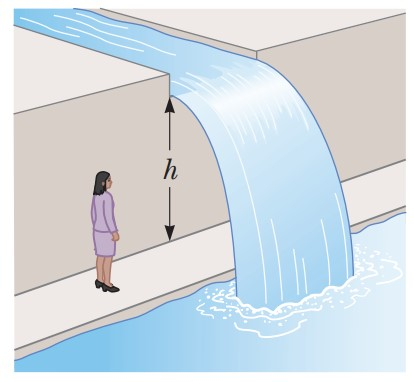
\includegraphics[scale=0.7]{../figs/G10-BTNEMNGANG2}}

	\loigiai{}
\end{ex}
% ======================================================================
\begin{ex}
	\immini{Một chiếc xe tải chở đầy dưa hấu dừng lại đột ngột để tránh lao xuống sông do cây cầu đã bị cuốn trôi. Việc dừng xe đột ngột khiến một số quả dưa văng khỏi xe tải. Một quả dưa rời khỏi mui xe tải với tốc độ ban đầu $v_i=\SI{10}{\meter/\second}$ theo phương ngang. Mặt cắt ngang của bờ sông có dạng nửa parabol $y^2=16x$, với đỉnh là vị trí ban đầu của quả dưa hấu và $x,y$ đều đo bằng mét. Quả dưa hấu va vào bờ sông ở tọa độ bằng bao nhiêu?	Lấy $g=\SI{9.8}{\meter/\second^2}$.}
	{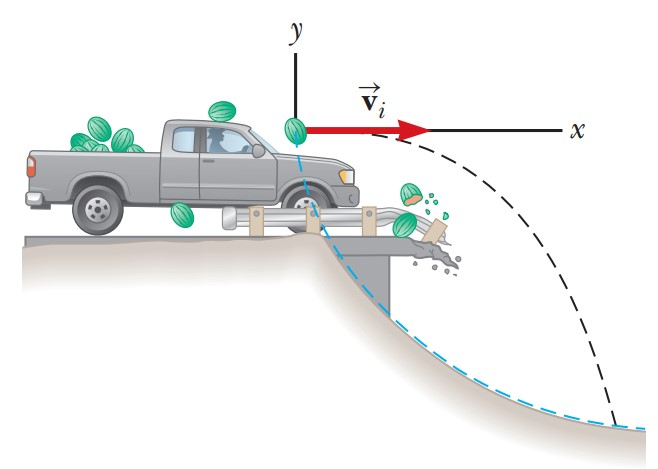
\includegraphics[scale=0.6]{../figs/G10-BTNEMNGANG2-2}}
	\loigiai{}
\end{ex}
% ======================================================================
\begin{ex}
\immini{Trong hình bên, bốn lá sen nhô lên khỏi mặt nước và một con ếch đang ở ngồi trên bờ hồ. Cho rằng độ cao của bờ hồ và lá sen so với mặt nước lần lượt là $H=6h$, $h_a=h_b=4h$, $h_c=h_d=h$. Ếch và tâm của hai lá sen a, b cùng nằm trên một mặt phẳng thẳng đứng. Giao điểm của thân bốn lá sen với mặt nước là bốn đỉnh của một hình vuông song song với bờ sông và có chiều dài cạnh bằng $\ell$. Khoảng cách theo phương ngang giữa lá sen a và bờ hồ cũng là $\ell$. Xem con ếch chuyển động như vật ném ngang với gia tốc trọng trường $g$.}
{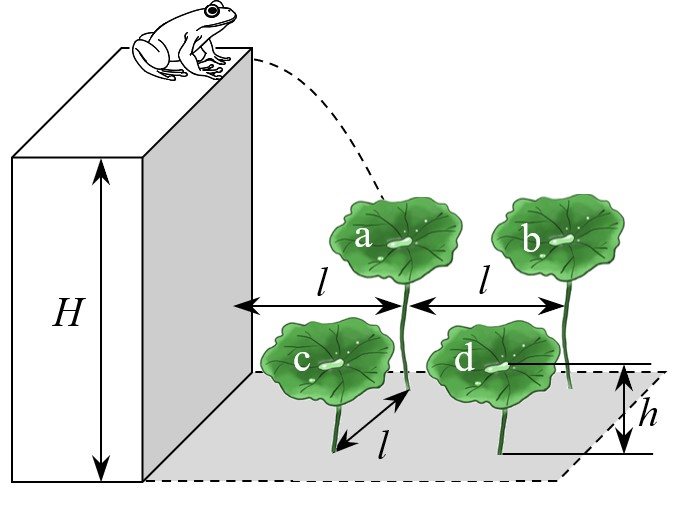
\includegraphics[scale=0.6]{../figs/G10-BTNEMNGANG2-5}}
\begin{enumerate}[label=\alph*)]
	\item Sau một cú nhảy, con ếch đã đậu thành công trên lá sen a. Tìm tốc độ ban đầu của con ếch.
	\item Tốc độ nhảy ban đầu của con ếch ứng với sự rơi trên lá sen nào là nhỏ nhất? Giải thích một cách tường minh.
\end{enumerate}
	\loigiai{}
\end{ex}
% ======================================================================
\begin{ex}
	\immini{Chó sói Wile E. Coyote cố gắng một lần nữa để bắt chú gà lôi thông minh Road Runner. Sói Wile E. mang một đôi giày trượt patin trợ lực mới để tạo ra gia tốc không đổi $\SI{15}{\meter/\second^2}$ trên phương ngang như hình bên. Con sói xuất phát từ trạng thái nghỉ cách mép vách đá $\SI{70}{\meter}$ vào thời điểm gà lôi vượt qua nó và lao về hướng vách đá. Lấy $g=\SI{9.8}{\meter/\second^2}$.
		\begin{enumerate}[label=\alph*)]
			\item Nếu gà lôi chạy với tốc độ không đổi, hãy tìm tốc độ tối thiểu của nó để đến được vách đá trước khi con sói bắt kịp.
			\item Nếu vách đá cao $\SI{100}{\meter}$ so với chân núi, hãy tìm nơi con sói rơi xuống. \textit{(Giả sử giày trượt của Wile E. vẫn còn hoạt động khi nó đang bay và thành phần phần gia tốc theo phương ngang anh ta vẫn bằng $\SI{15}{\meter/\second^2}$ không đổi).}
	\end{enumerate}}
	{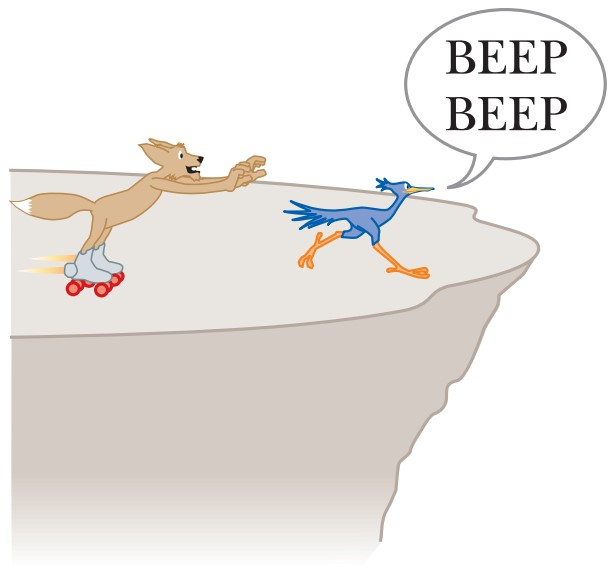
\includegraphics[scale=0.6]{../figs/G10-BTNEMNGANG2-4}}
	
	\loigiai{}
\end{ex}
% ======================================================================
\begin{ex}
	\immini{Một máy bay ném bom, bay theo phương ngang ở độ cao $H=\SI{500}{\meter}$ so với mặt đất, chuyển động nhanh dần đều với gia tốc $a=\SI{2}{\meter/\second^2}$ và các quả bom được thả sau những khoảng thời gian bằng nhau $t=\SI{0.5}{\second}$. Tìm khoảng cách giữa các điểm rơi của quả bom thứ 9 và thứ 11 trên mặt đất nếu quả bom thứ nhất được thả ra khi vận tốc của máy bay là $v_0=\SI{100}{\meter/\second}$. Cho $g=\SI{10}{\meter/\second^2}$ và bỏ qua sức cản của không khí.}
	{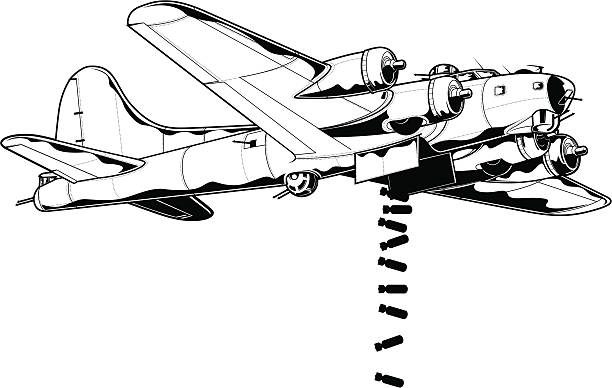
\includegraphics[scale=0.7]{../figs/G10-BTNEMNGANG2-3}}
	\loigiai{$\Delta s=L+s_{11}-s_9=\SI{129}{\meter}$.}
\end{ex}
	% ======================== ÔN TẬP GKI
%	\begin{center}
	\begin{tabular}{M{9.25cm}M{8.75cm}}
		\textbf{TRƯỜNG THCS-THPT NGUYỄN KHUYẾN}& \textbf{ÔN TẬP GIỮA HỌC KÌ 1}\\
		\textbf{MÃ ĐỀ: 001}& \textbf{Bài thi môn: VẬT LÝ 10}\\
		\textit{(Đề thi có 06 trang)}& \textit{Thời gian làm bài: 45 phút, không kể phát đề}
		
		\noindent\rule{4cm}{0.8pt} \\
	\end{tabular}
\end{center}
\setcounter{section}{0}
\begin{center}
	\textbf{\large BẢNG ĐÁP ÁN}
\end{center}
\section{}
\inputansbox{10}{ans/D10-GKI-001-TN}
\section{}
\inputansbox[2]{2}{ans/D10-GKI-001-TF}
\section{}
\inputansbox[3]{6}{ans/D10-GKI-001-TL}
%	\begin{center}
	\begin{tabular}{M{9.25cm}M{8.75cm}}
		\textbf{TRƯỜNG THCS-THPT NGUYỄN KHUYẾN}& \textbf{ÔN TẬP GIỮA HỌC KÌ 1}\\
		\textbf{MÃ ĐỀ: 001}& \textbf{Bài thi môn: VẬT LÝ 10}\\
		\textit{(Đề thi có 06 trang)}& \textit{Thời gian làm bài: 45 phút, không kể phát đề}
		
		\noindent\rule{4cm}{0.8pt} \\
	\end{tabular}
\end{center}
\setcounter{section}{0}
\section{Câu trắc nghiệm nhiều phương án lựa chọn}
\textit{Thí sinh trả lời từ câu 1 đến câu 20. Mỗi câu hỏi thí sinh chọn một phương án}
\setcounter{ex}{0}
\Opensolutionfile{ans}[ans/D10-GKI-001-TN]
% ===================================================================
\begin{ex}
Công thức tính tốc độ trung bình là	
	\choice
	{\True $v_{\text{tb}}=\dfrac{s}{t}$}
	{$v_{\text{tb}}=\dfrac{t}{s}$}
	{$v_{\text{tb}}=st$}
	{$v_{\text{tb}}=st^2$}
	\loigiai{}
\end{ex}
% ===================================================================
\begin{ex}
Một vật chuyển động thẳng biến đổi. Tại thời điểm $t_0$ vận tốc của vật là $v_0$, tại thời điểm $t$ vật có vận tốc $v$. Công thức tính gia tốc trung bình của vật là	
	\choice
	{\True $a_{\text{tb}}=\dfrac{v-v_0}{t-t_0}$}
	{$a_{\text{tb}}=\dfrac{v+v_0}{t-t_0}$}
	{$a_{\text{tb}}=\dfrac{v-v_0}{t+t_0}$}
	{$a_{\text{tb}}=\dfrac{v+v_0}{t+t_0}$}
	\loigiai{}
\end{ex}
% ===================================================================
\begin{ex}
	Chọn phát biểu \textbf{đúng}.
	\choice
	{Vận tốc tức thời cho ta biết chiều chuyển động của vật nên luôn có giá trị dương}
	{Vector độ dịch chuyển thay đổi phương liên tục khi vật chuyển động thẳng}
	{\True Khi vật chuyển động thẳng không đổi chiều, độ lớn của vector độ dịch chuyển bằng quãng đường vật đi được}
	{Vector độ dịch chuyển có độ lớn luôn bằng quãng đường đi được của chất điểm}
	\loigiai{}
\end{ex}
% ===================================================================
\begin{ex}
	Tốc độ là đại lượng đặc trưng cho
	\choice
	{\True tính chất nhanh hay chậm của chuyển động}
	{sự thay đổi hướng của chuyển động}
	{khả năng duy trì chuyển động của vật}
	{sự thay đổi vị trí của vật trong không gian}
	\loigiai{}
\end{ex}
% ===================================================================
\begin{ex}
	\immini{
		Biển báo giao thông như hình bên (viền đỏ, nền trắng) cho biết
		\choice
		{các loại xe có khối lượng không quá $\SI{50}{\kilogram}$ mới được lưu thông}
		{tài xế có cân nặng trên $\SI{50}{\kilo\gram}$ mới được điều khiển các loại xe cơ giới}
		{các loại xe cơ giới (trừ xe ưu tiên) không được chạy quá $\SI{50}{\kilo\meter/\hour}$}
		{còn $\SI{50}{\meter}$ nữa sẽ đến khúc cua nguy hiểm}
	}
	{
	
\includegraphics[width=0.4\linewidth]{../figs/D10-1-6}
	}
	\loigiai{}
\end{ex}
% ===================================================================
\begin{ex}
	Chuyển động thẳng chậm dần đều là chuyển động có
	\choice
	{tốc độ giảm đều, gia tốc giảm đều}
	{vận tốc không đổi, gia tốc giảm đều}
	{\True tốc độ giảm đều, gia tốc không đổi}
	{vận tốc không đổi, gia tốc không đổi}
	\loigiai{}
\end{ex}
% ===================================================================
\begin{ex}
	Chuyển động nhanh dần có đặc điểm
	\choice
	{$\vec{a}$ ngược chiều $\vec{v}$}
	{$a<0$, $v>0$}
	{\True $\vec{a}$ cùng chiều $\vec{v}$}
	{$a>0$, $v<0$}
	\loigiai{}
\end{ex}
% ===================================================================
\begin{ex}
	Dựa vào độ dốc của đồ thị độ dịch chuyển - thời gian có thể xác định đại lượng nào sau đây?
	\choice
	{\True Vận tốc}
	{Gia tốc}
	{Độ dịch chuyển}
	{Khoảng thời gian}
	\loigiai{}
\end{ex}
% ===================================================================
\begin{ex}
	Chọn phát biểu \textbf{đúng}.
	\choice
	{Vận tốc là đại lượng vô hướng không âm}
	{Vận tốc là đại lượng vector có hướng ngược hướng với hướng của độ dịch chuyển}
	{Vận tốc là đại lượng vô hướng có thể âm hoặc dương}
	{\True Vận tốc là đại lượng vector có hướng là hướng của độ dịch chuyển}
	\loigiai{}
\end{ex}
% ===================================================================
\begin{ex}
	\immini{
	Một xe ô tô đồ chơi chuyển động trên đường thẳng có đồ thị độ dịch chuyển - thời gian như hình bên. Tốc độ của xe ô tô đồ chơi tại thời điểm $
	\SI{10}{\second}$ là
	\choice
	{$\SI{0.7}{\meter/\second}$}
	{\True $\SI{1.5}{\meter/\second}$}
	{$\SI{0}{\meter/\second}$}
	{$\SI{1.0}{\meter/\second}$}
	}
	{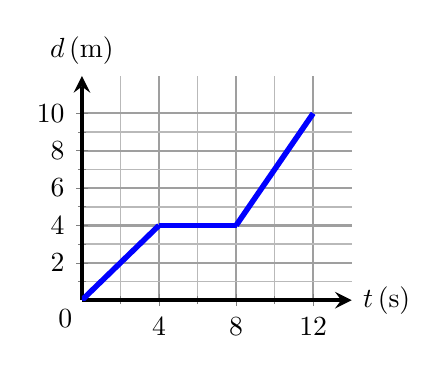
\begin{tikzpicture}  
			\begin{axis}[  ultra thick,scale=0.5,
				xmin=0,  
				xmax=14,  
				xtick={0,4,...,12},
				ytick={0,2,...,10},
				minor x tick num=1,
				minor y tick num=1,
				ymin=0,  
				ymax=12, 
				samples=300,
				axis lines=center, 
				grid style={step=1, line width =0.6pt, color=gray!55!white},
				grid=both, %giới hạn ô lưới
				major grid style={line width=0.8pt,gray!75!white},
				xlabel=$\xsi{t}{\left(\si{\second}\right)}$, 		ylabel=$\xsi{d}{\left(\si{\meter}\right)}$,
				every axis y label/.style={at=(current axis.above origin),anchor=south},  
				every axis x label/.style={at=(current axis.right of origin),anchor=west},  ]
				\addplot [line width=2pt, blue, smooth, domain=0:4] {x};  
				\addplot [line width=2pt, blue, smooth, domain=4:8] {4};
				\addplot [line width=2pt, blue, smooth, domain=8:12] {4+1.5*(x-8)};
				\coordinate (O) at (axis cs: 0,0);
			\end{axis}  
			\node[below left] at (O) {0};
	\end{tikzpicture}}
	\loigiai{}
\end{ex}
% ===================================================================
\begin{ex}
	Một vật chuyển động thẳng có đồ thị vận tốc theo thời gian như hình vẽ. Giai đoạn vật chuyển động thẳng nhanh dần đều là
	\begin{center}
		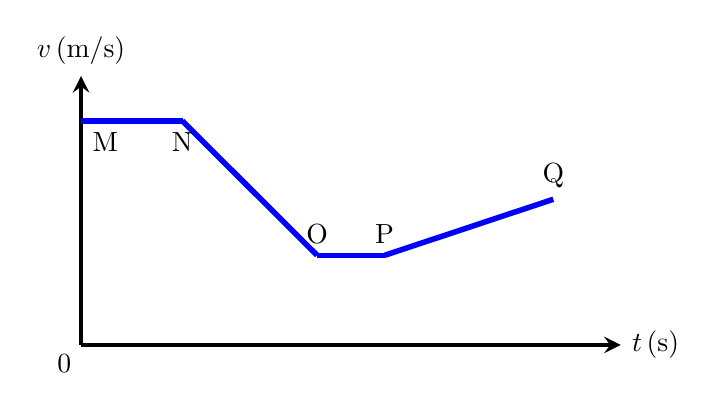
\begin{tikzpicture}  
			\begin{axis}[  ultra thick,yscale=0.6,
				xmin=0,  
				xmax=16,  
				ymin=0,  
				ymax=6, 
				samples=300,
				yticklabels=\empty,
				xticklabels=\empty,
				xtick=\empty,
				ytick=\empty,
				axis lines=center, 
				xlabel=$\xsi{t}{\left(\si{\second}\right)}$, 		ylabel=$\xsi{v}{\left(\si{\meter/\second}\right)}$,
				every axis y label/.style={at=(current axis.above origin),anchor=south},  
				every axis x label/.style={at=(current axis.right of origin),anchor=west},  ]
				\coordinate (M) at (axis cs: 0,5);
				\coordinate (N) at (axis cs: 3,5);
				\coordinate (OO) at (axis cs: 7,2);
				\coordinate (P) at (axis cs: 9,2);
				\coordinate (Q) at (axis cs: 14,3.25);
				\addplot [line width=2pt, blue, smooth, domain=0:3] {5}; 
				\addplot [line width=2pt, blue, smooth, domain=3:7] {5-0.75*(x-3)}; 
				\addplot [line width=2pt, blue, smooth, domain=7:9] {2}; 
				\addplot [line width=2pt, blue, smooth, domain=9:14] {2+0.25*(x-9)};
				\coordinate (O) at (axis cs: 0,0);
				\node[below right] at (M) {M};
				\node[below] at (N) {N};
				\node[above] at (OO) {O};
				\node[above] at (P) {P};
				\node[above] at (Q) {Q};
			\end{axis}  
			\node[below left] at (O) {0};
		\end{tikzpicture}
	\end{center}
	\choice
	{MN}
	{NO}
	{OP}
	{\True PQ}
	\loigiai{}
\end{ex}

% ===================================================================
\begin{ex}
	Bạn Bình đi học từ nhà đến trường theo lộ trình ABC như hình vẽ. Biết bạn Bình đi đoạn đường $\mathrm{AB}=\SI{400}{\meter}$ hết 6 phút, đoạn đường $\mathrm{BC}=\SI{300}{\meter}$ hết 4 phút. Vận tốc trung bình của bạn Bình khi đi từ nhà đến trường là
	\begin{center}
		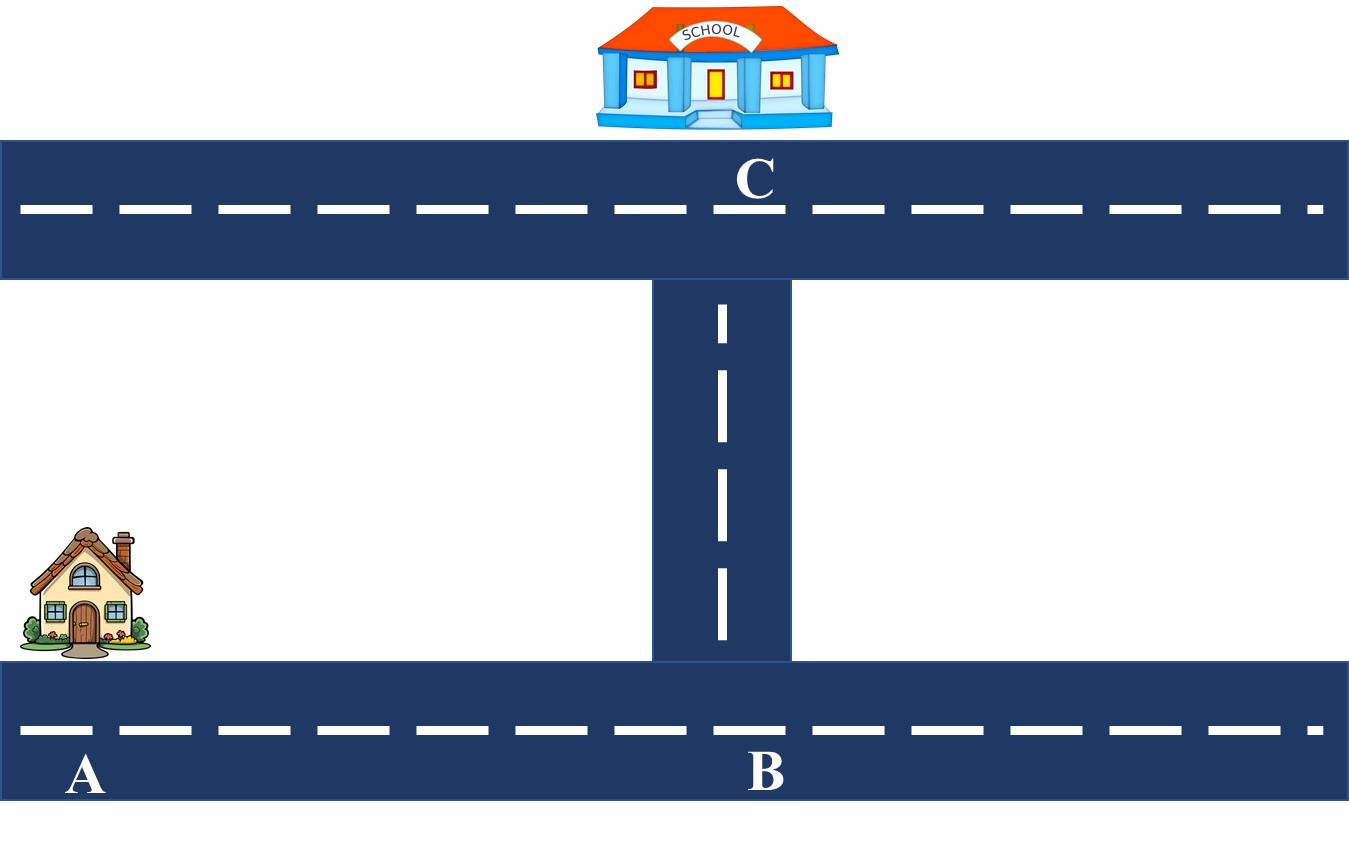
\includegraphics[width=0.4\linewidth]{../figs/D10-1-3}
	\end{center}
	\choice
	{\True $\SI{0.833}{\meter/\second}$}
	{$\SI{2.916}{\meter/\second}$}
	{$\SI{1.167}{\meter/\second}$}
	{$\SI{3.512}{\meter/\second}$}
	\loigiai{
	$$v=\dfrac{\mathrm{AC}}{t_{\mathrm{AB}}+t_{\mathrm{BC}}}\approx\SI{0.833}{\meter/\second}.$$
	}
\end{ex}
% ===================================================================
\begin{ex}
	Giờ Phối hợp Quốc tế (UTC) là tiêu chuẩn thời gian được sử dụng rộng rãi trên thế giới. So với 0 giờ Quốc Tế, Việt Nam ở múi giờ thứ 7 (UTC +7) và Nhật Bản ở múi giờ thứ 9 (UTC +9). Ngày 10/02/2024, máy bay VN300, thuộc hãng hàng không Vietnam Airlines, khởi hành từ Thành phố Hồ Chí Minh lúc 0 giờ 20 phút và đến Thành phố Tokyo lúc 7 giờ 45 phút, theo giờ địa phương. Thời gian di chuyển của máy bay này là
	\choice
	{5 giờ 25 phút}
	{\True 9 giờ 25 phút}
	{7 giờ 25 phút}
	{8 giờ 05 phút}
	\loigiai{
	}
\end{ex}

% ===================================================================
\begin{ex}
	Biểu thức nào sau đây đang mô tả vận tốc của vật chuyển động thẳng chậm dần đều?
	\choice
	{\True $v=-20+5t\ \left(\si{\meter/\second}; \si{\second}\right)$}
	{$v=10+5t\ \left(\si{\meter/\second}; \si{\second}\right)$}
	{$v=5t\ \left(\si{\meter/\second}; \si{\second}\right)$}
	{$v=-20-5t\ \left(\si{\meter/\second}; \si{\second}\right)$}
	\loigiai{}
\end{ex}
% ===================================================================
\begin{ex}
	Một vật chuyển động thẳng nhanh dần đều với tốc độ đầu là $\SI{6}{\meter/\second}$ và độ lớn gia tốc là $\SI{2}{\meter/\second^2}$. Chọn thời điểm ban đầu là lúc vật ở gốc tọa độ và chiều dương ngược chiều chuyển động thì phương trình chuyển động của vật có dạng
	\choice
	{$x=6t-t^2\ \left(\si{\meter}; \si{\second}\right)$}
	{$x=6t-2t^2\ \left(\si{\meter}; \si{\second}\right)$}
	{\True $x=-6t-t^2\ \left(\si{\meter}; \si{\second}\right)$}
	{$x=-6t-2t^2\ \left(\si{\meter}; \si{\second}\right)$}
	\loigiai{}
\end{ex}
% ===================================================================
\begin{ex}
	Một xe đi nửa đoạn đường đầu tiên với tốc độ trung bình
	 $v_1=\SI{12}{\kilo\meter/\hour}$ và nửa đoạn đường	sau với tốc độ trung bình $v_2=\SI{20}{\kilo\meter/\hour}$. Tốc độ trung bình của xe trên cả đoạn đường là
	\choice
	{$\SI{30}{\kilo\meter/\hour}$}
	{\True $\SI{15}{\kilo\meter/\hour}$}
	{$\SI{16}{\kilo\meter/\hour}$}
	{$\SI{32}{\kilo\meter/\hour}$}
	\loigiai{
	$$v_{\text{tb}}=\dfrac{2s}{\dfrac{s}{v_1}+\dfrac{s}{v_2}}=\dfrac{2}{\dfrac{1}{v_1}+\dfrac{1}{v_2}}=\SI{15}{\kilo\meter/\hour}.$$
	}
\end{ex}
% ===================================================================
\begin{ex}
	Một ô tô đang chạy với vận tốc $\SI{72}{\kilo\meter/\hour}$ trên một đoạn đường thắng thì người lái xe hãm phanh cho ô tô chạy chậm dần. Sau $\SI{40}{\second}$, ô tô dừng lại. Gia tốc của ô tô là
	\choice
	{$a=\SI{-0.2}{\meter/\second^2}$}
	{\True $a=\SI{-0.5}{\meter/\second^2}$}
	{$a=\SI{0.2}{\meter/\second^2}$}
	{$a=\SI{-1}{\meter/\second^2}$}
	\loigiai{
	$$a=\dfrac{v-v_0}{\Delta t}=\dfrac{0-20}{40}=\SI{-0.5}{\meter/\second^2}.$$
	}
\end{ex}

% ===================================================================
\begin{ex}
	Một xe máy đang chạy với tốc độ $\SI{36}{\kilo\meter/\hour}$ bỗng người lái xe thấy có một cái hố trước mặt, cách xe $\SI{20}{\meter}$. Người ấy phanh gấp và xe đến ngay trước miệng hố thì dừng lại. Gia tốc của xe máy có độ lớn là 
	\choice
	{$\SI{5.09}{\meter/\second^2}$}
	{$\SI{4.1}{\meter/\second^2}$}
	{\True $\SI{2.5}{\meter/\second^2}$}
	{$\SI{32.4}{\meter/\second^2}$}
	\loigiai{}
\end{ex}

% ===================================================================
\begin{ex}
	Một vật chuyển động trên đường thẳng có phương trình vận tốc - thời gian $v=-5+5t\ \left(\si{\meter/\second};\si{\second}\right)$. Tại thời điểm $t=\SI{10}{\second}$ thì quãng đường vật đã đi \textbf{gần nhất} với giá trị nào?
	\choice
	{$\SI{400}{\meter}$}
	{$\SI{300}{\meter}$}
	{$\SI{100}{\meter}$}
	{\True $\SI{200}{\meter}$}
	\loigiai{
	Thời điểm vật đổi chiều chuyển động: $v=0\Rightarrow t=\SI{1}{\second}$.\\
	Trong 1 giây đầu vật chuyển động chậm dần đều ngược chiều dương với vận tốc đầu $v_0=\SI{-5}{\meter/\second}$ và gia tốc $a=\SI{5}{\meter/\second^2}$: $d=v_0t+\dfrac{1}{2}at^2=\SI{-2.5}{\meter}\Rightarrow s=\SI{2.5}{\meter}$.\\
	Trong 9 giây còn lại vật chuyển động nhanh dần theo chiều dương với gia tốc $a=\SI{5}{\meter/\second^2}$:
	$s'=\dfrac{1}{2}at'^2=\SI{202.5}{\meter}$.\\
	Vậy tổng quãng đường dịch chuyển là $s+s'=\SI{205}{\meter}$.
	}
\end{ex}


% ===================================================================
\begin{ex}
Các giọt nước mưa rơi từ một đám mây; khi xuống tới gần mặt đất	coi giọt mưa rơi thẳng đứng với tốc độ không đổi $\SI{30}{\meter/\second}$, lúc này giọt nước đập vào tấm kính ở cửa bên của một ô tô đang chuyển động thẳng đều theo phương ngang, giọt mưa để lại trên kính một vết nước hợp với phương thẳng đứng một góc $\SI{30}{\degree}$. Tốc độ của ô tô \textbf{gần nhất} với giá trị nào sau đây?
	\choice
	{\True $\SI{62.4}{\kilo\meter/\hour}$}
	{$\SI{108}{\kilo\meter/\hour}$}
	{$\SI{54.8}{\kilo\meter/\hour}$}
	{$\SI{72.5}{\kilo\meter/\hour}$}
	\loigiai{
	$$v_{\text{xe}}=v_{\text{mưa}}\cdot\tan\SI{30}{\degree}\approx\SI{62,4}{\kilo\meter/\hour}.$$
	}
\end{ex}


\Closesolutionfile{ans}
\section{Câu trắc nghiệm đúng/sai} 
\textit{Thí sinh trả lời từ câu 1 đến câu 2. Trong mỗi ý \textbf{a)}, \textbf{b)}, \textbf{c)}, \textbf{d)} ở mỗi câu, thí sinh chọn đúng hoặc sai}
\setcounter{ex}{0}
\Opensolutionfile{ans}[ans/D10-GKI-001-TF]

% ===================================================================
\begin{ex}
	Trong một tình huống bóng đá, thủ môn xuất phát từ vạch ngang nối hai cột của khung thành chạy thẳng lên phía trước để bắt bóng. Hình bên là đồ thị độ dịch chuyển - thời gian của thủ môn. Điểm A tương ứng với điểm xuất phát, đoạn AB có dạng parabol, BC là đoạn thẳng.
	\begin{center}
		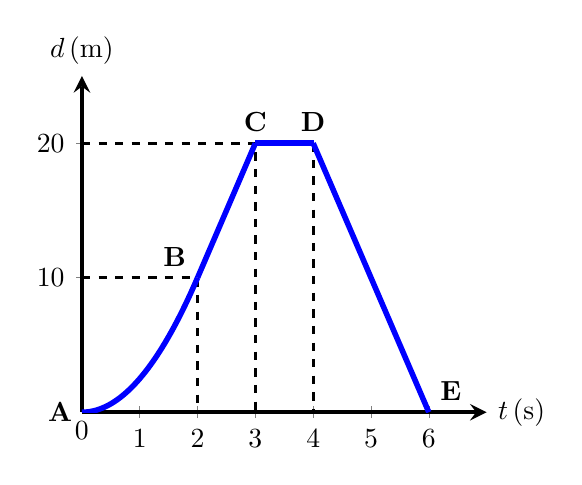
\begin{tikzpicture}  
			\begin{axis}[  ultra thick,scale=0.75,
				xmin=0,  
				xmax=7,  
				xtick={0,1,...,6},
				ytick={0,10,20},
				minor x tick num=0,
				minor y tick num=0,
				ymin=0,  
				ymax=25, 
				samples=300,
				axis lines=center, 
				xlabel=$\xsi{t}{\left(\si{\second}\right)}$, 		ylabel=$\xsi{d}{\left(\si{\meter}\right)}$,
				every axis y label/.style={at=(current axis.above origin),anchor=south},  
				every axis x label/.style={at=(current axis.right of origin),anchor=west},  ]
				\draw[dashed, line width=1pt] (axis cs: 0,10)--(axis cs: 2,10)--(axis cs: 2,0);
				\draw[dashed, line width=1pt] (axis cs: 0,20)--(axis cs: 3,20)--(axis cs: 3,0);
				\draw[dashed, line width=1pt] (axis cs: 4,20)--(axis cs: 4,0);
				\addplot [line width=2pt, blue, smooth, domain=0:2] {0.5*5*x^(2)}; 
				\addplot [line width=2pt, blue, smooth, domain=2:3] {10+10*(x-2)};  
				\addplot [line width=2pt, blue, smooth, domain=3:4] {20}; 
				\addplot [line width=2pt, blue, smooth, domain=4:6] {20-10*(x-4)};
				\coordinate (O) at (axis cs: 0,0);
				\coordinate (A) at (axis cs: 0,0);
				\coordinate (B) at (axis cs: 2,10);
				\coordinate (C) at (axis cs: 3,20);
				\coordinate (D) at (axis cs: 4,20);
				\coordinate (E) at (axis cs: 6,0);
				\node[above left] at (B) {\textbf{B}};
				\node[above] at (C) {\textbf{C}};
				\node[above] at (D) {\textbf{D}};
				\node[above right] at (E) {\textbf{E}};
			\end{axis}  
			\node[below] at (O) {0};
			\node[left] at (A) {\textbf{A}};
		\end{tikzpicture}
	\end{center}
	\choiceTF[t]
	{Trong khoảng thời gian từ $\SI{0}{\second}$ đến $\SI{6}{\second}$ thủ môn không đổi hướng chuyển động}
	{\True Thủ môn tăng tốc trong khoảng thời gian từ $\SI{0}{\second}$ đến $\SI{2}{\second}$}
	{\True Tốc độ chuyển động của thủ môn từ điểm B đến điểm C là $\SI{10}{\meter/\second}$}
	{\True Từ 4 giây đến 6 giây, vận tốc chuyển động của thủ môn có giá trị $\SI{-10}{\meter/\second}$}
	\loigiai{}
\end{ex}
% ===================================================================
\begin{ex}
Khi xe chạy trên đường cao tốc, xe phải giữ khoảng cách an toàn với xe phía trước để có thể xử lý kịp thời khi xe phía trước gặp sự cố.
\begin{center}
	
\includegraphics[width=0.4\linewidth]{../figs/D10-1-4}
\end{center}	
Khoảng cách an toàn này tùy thuộc vào tốc độ xe và đã được nêu trong một số quy định của chính phủ. Tuy nhiên, để dễ nhớ, khi lưu thông vào ban ngày và khi đường khô ráo người ta thường tính toán theo một trong các quy tắc sau:
\begin{itemize}
	\item \textbf{\textit{Quy tắc 1:}} Quy tắc $\SI{3}{\second}$  tối thiểu. Khoảng cách an toàn tối thiểu bằng quãng đường xe đi được trong $\SI{3}{\second}$. Ví dụ xe chạy với tốc độ $\SI{72}{\kilo\meter/\hour}$  thì khoảng cách an toàn tối thiểu với xe phía trước là $\SI{60}{\meter}$.
	\item \textbf{\textit{Quy tắc 2:}} Quy tắc tương đương. Khoảng cách an toàn tối thiểu (theo đơn vị $\si{\meter}$) bằng tốc độ của xe (theo đơn vị $\si{\kilo\meter/\hour}$). Ví dụ tốc độ xe là $\SI{80}{\kilo\meter/\hour}$  thì khoảng cách an toàn tối thiểu với xe phía trước là $\SI{80}{\meter}$.
\end{itemize}
Một xe ô tô đang chạy trên đường cao tốc nằm ngang với tốc độ $\SI{108}{\kilo\meter/\hour}$  thì bất ngờ thấy một sự cố trên đường ở phía trước, sau đó $\SI{1}{\second}$ thì tài xế ô tô bắt đầu giảm hẳn ga và thắng gấp xe lại với gia tốc có độ lớn $\SI{8}{\meter/\second^2}$ cho đến khi xe ngừng lại.
	\choiceTF[t]
	{\True Theo quy tắc 1, khoảng cách an toàn tối thiểu với trường hợp xe ô tô trên là $\SI{90}{\meter}$}
	{Theo quy tắc 2, khoảng cách an toàn tối thiểu với trường hợp xe ô tô trên là $\SI{30}{\meter}$}
	{\True Tổng quãng đường ô tô đi được từ lúc phát hiện sự cố đến khi dừng lại $\SI{86.25}{\meter}$}
	{\True Nếu sự cố mà xe ô tô nhìn thấy là một xe container phía trước, đang chuyển động cùng chiều, thẳng đều, với tốc độ $\SI{36}{\kilo\meter/\hour}$ thì khoảng cách tối thiểu của hai xe kể từ lúc người lái ô tô thắng lại phải là $\SI{25}{\meter}$ để không xảy ra tai nạn. }
	\loigiai{
	\begin{itemchoice}
		\itemch Đúng.
		\itemch Sai. Theo quy tắc 2, khoảng cách an toàn tối thiểu là $\SI{108}{\meter}$.
		\itemch Đúng.\\
		Trong quá trình từ khi ô tô thấy sự cố đến khi thắng lại, ô tô chuyển động thẳng đều. Quãng đường ô tô đi được trong quá trình trên: $s_1=v_0t=30\cdot1=\SI{30}{\meter}$.\\
		Trong quá trình ô tô thắng lại, ô tô chuyển động chậm dần đều với vận tốc đầu $v_0$. Đến khi dừng lại  $v=0$.\\
		Quãng đường ô tô đi được trong quá trình này: $s_2=\dfrac{v^2-v^2_0}{2a}=\SI{56.25}{\meter}$.\\
		Tổng quãng đường ô tô đi được từ lúc phát hiện sự cố đến khi dừng lại: $s=s_1+s_2=\SI{86.25}{\meter}$.
		\itemch Đúng.\\
		Chọn trục tọa độ  gắn với xe con, chiều dương $Ox$ cùng chiều chuyển động của xe, gốc tọa độ O trùng với điểm B, gốc thời gian lúc ô tô bắt đầu hãm phanh.\\
		Phương trình chuyển động của ô tô: $x_1=-\mathrm{AB}+v_{01}t-\dfrac{1}{2}at^2$.\\
		Phương trình chuyển động của xe container:  $x_2=v_2t$.\\
		Nếu hai xe va chạm (gặp nhau): 
		$$x_1=x_1\Rightarrow \mathrm{AB}+\left(v_2-v_{01}\right)t+\dfrac{1}{2}at^2=0 \quad \left(*\right)$$
		Để ô tô chỉ gặp xe container một lần và dừng lại ngay trước khi va chạm, hoặc không gặp xe container (không xảy ra tai nạn) thì phương trình (*) phải có không quá một nghiệm thực, khi đó biệt số $\Delta $:
		$$\Delta \le 0\Leftrightarrow \left(v_2-v_{01}\right)^2-2a\cdot\mathrm{AB}\le 0$$
		$$\Rightarrow \mathrm{AB}\ge \dfrac{\left(v_2-v_{01}\right)^2}{2a}$$
		$$\Rightarrow \mathrm{AB}_{\text{min}}=\dfrac{\left(v_2-v_{01}\right)^2}{2a}=\SI{25}{\meter}.$$
	\end{itemchoice}
	}
\end{ex}
\Closesolutionfile{ans}

\section{Câu trắc nghiệm trả lời ngắn} \textit{Thí sinh trả lời từ câu 1 đến câu 6}
\setcounter{ex}{0}
\Opensolutionfile{ans}[ans/D10-GKI-001-TL]
% ===============================================================
\begin{ex}
	Một vận động viên chạy từ điểm xuất phát lên một quả đồi với tốc độ không đổi $\SI{3}{\meter/\second}$. Khi chạy được $\SI{90}{\meter}$ thì vận động viên này lập tức chạy ngược lại theo đường cũ về điểm xuất phát với tốc độ không đổi $\SI{6}{\meter/\second}$. Ở cả hành trình trên, tốc độ trung bình của vận động viên là bao nhiêu $\si{\meter/\second}$?
	\shortans{4 }
	\loigiai{
		$$v_{\text{tb}}=\dfrac{2s}{\dfrac{s}{v_1}+\dfrac{s}{v_2}}=\SI{4}{\meter/\second}.$$
	}
\end{ex}
% ===============================================================
\begin{ex}
	Một quả bóng tennis đang bay với tốc độ $\SI{25}{\meter/\second}$ theo hướng đông thì chạm vào tường chắn và bay trở lại với tốc độ $\SI{15}{\meter/\second}$ theo hướng tây. Thời gian va chạm giữa tường và bóng là $\SI{0.05}{\second}$. Tính gia tốc của quả bóng trong thời gian tiếp xúc với tường theo đơn vị $\si{\meter/\second^2}$. Chọn chiều dương là chiều chuyển động ban đầu của quả bóng.
	\shortans{-800 }
	\loigiai{
	}
\end{ex}
% ===============================================================
\begin{ex}
	Trong một thí nghiệm đo tốc độ chuyển động của vật nhỏ bằng đồng hồ cần rung, người ta đã thu được một băng giấy với các dấu mực như hình vẽ bên dưới. Thước đo được sử dụng trong hình vẽ là thước đo $\si{\centi\meter}$. Biết rằng khoảng thời gian giữa các lần chấm mực luôn bằng nhau và bằng $\SI{0.2}{\second}$. Trong khoảng thời gian giữa lần chấm mực đầu tiên (đánh số 1) cho đến lần chấm mực cuối cùng (đánh số 8) thì tốc độ trung bình của vật nhỏ đó bằng bao nhiêu $\si{\centi\meter/\second}$?	
	\begin{center}
		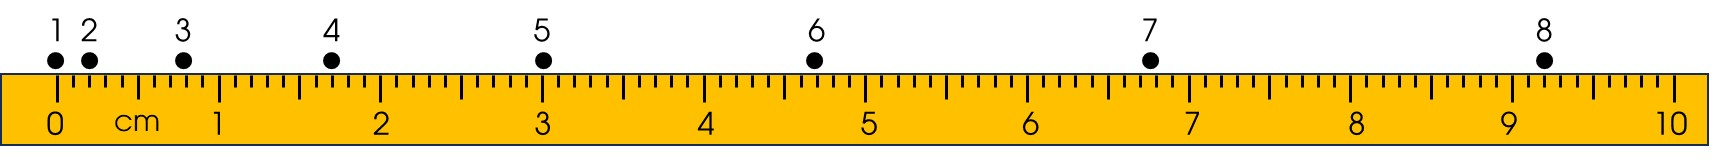
\includegraphics[width=0.9\linewidth]{../figs/D10-2-15}
	\end{center}
	\shortans{6,57}
	\loigiai{
		
	}
\end{ex}

% ===============================================================
\begin{ex}
Một vật chuyển động thẳng có đồ thị vận tốc - thời gian như hình bên dưới. Tính tổng quãng đường vật đi được trong khoảng thời gian $\SI{12}{\second}$ theo đơn vị mét.
\begin{center}
	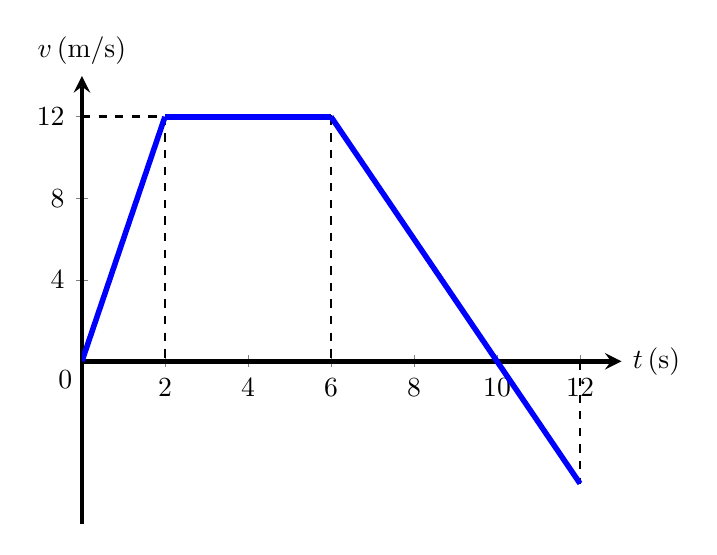
\begin{tikzpicture}  
		\begin{axis}[  ultra thick,
			xmin=0,  
			xmax=13,  
			xtick={0,2,...,12},
			ytick={0,4,...,12},
			ymin=-8,  
			ymax=14, 
			samples=300,
			axis lines=center, 
			xlabel=$\xsi{t}{\left(\si{\second}\right)}$, 		ylabel=$\xsi{v}{\left(\si{\meter/\second}\right)}$,
			every axis y label/.style={at=(current axis.above origin),anchor=south},  
			every axis x label/.style={at=(current axis.right of origin),anchor=west},  ]
			\draw[dashed, line width=1pt] (axis cs: 0,12)--(axis cs: 2,12)--(axis cs: 2,0);
			\draw[dashed, line width=1pt] (axis cs: 0,12)--(axis cs: 6,12)--(axis cs: 6,0);
			\draw[dashed, line width=1pt] (axis cs: 12,0)--(axis cs: 12,-6);
			\addplot [line width=2pt, blue, smooth, domain=0:2] {6*x}; 
			\addplot [line width=2pt, blue, smooth, domain=2:6] {12};  
			\addplot [line width=2pt, blue, smooth, domain=6:12] {12-3*(x-6)}; 
			\coordinate (O) at (axis cs: 0,0);
		\end{axis}  
		\node[below left] at (O) {0};
	\end{tikzpicture}
\end{center}	
	\shortans{$90$ }
	\loigiai{
		$$s=\dfrac{1}{2}\cdot\left(4+10\right)\cdot12+\dfrac{1}{2}\cdot2\cdot6=\SI{90}{\meter}.$$
	}
\end{ex}
% ===================================================================
\begin{ex}
	Một người đi xe đạp với tốc độ $v_1=\SI{5}{\meter/\second}$ bên cạnh đường ray tàu hỏa thì thấy một chiếc tàu hỏa chạy qua cùng chiều. Tốc độ của tàu hỏa là $v_2=\SI{15}{\meter/\second}$ đối với mặt đất. Sau thời gian $\SI{15}{\second}$ thì người đó thấy tàu hỏa vượt qua mặt mình. Chiều dài của tàu hỏa là bao nhiêu mét?
	\begin{center}
		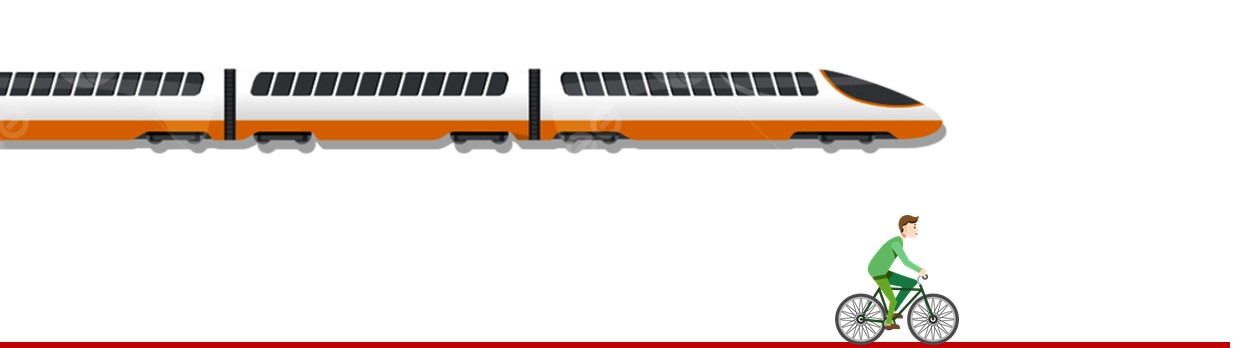
\includegraphics[width=0.5\linewidth]{../figs/D10-1-2}
	\end{center}
\shortans{150}
	\loigiai{
		Vận tốc tương đối của tàu hỏa so với người:
		$$v_{21}=v_2-v_1=\SI{10}{\meter/\second}$$
		Chiều dài của tàu hỏa:
		$$L=v_{21}t=\SI{150}{\meter}.$$
	}
\end{ex}
% ===================================================================
\begin{ex}
	\immini{
		Trong khi làm thí nghiệm với đồng hồ đo thời gian hiện số, một học sinh chọn kiểu làm việc (MODE) của đồng hồ ở vị trí A và nối cổng quang điện với ổ A của đồng hồ. Học sinh này thả rơi một thước nhôm dài $\SI{20}{\centi\meter}$ theo phương thẳng đứng sao cho thước rơi qua cổng quang điện (thước luôn thẳng đứng khi rơi) thì thấy số chỉ của đồng hồ bằng $\SI{0.077}{\second}$. 
	}
	{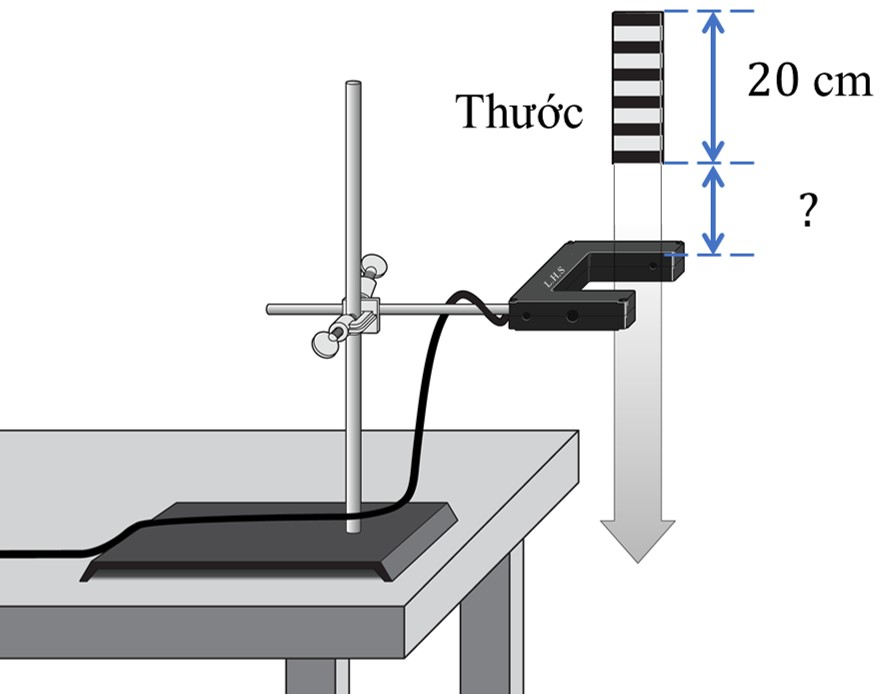
\includegraphics[width=0.6\linewidth]{../figs/D10-1-1}}
	Bỏ qua sức cản của không khí và thước chuyển động nhanh dần đều với gia tốc có độ lớn $\SI{9.8}{\meter/\second^2}$. Khi thả, đầu dưới của thước cách cổng quang điện một khoảng bằng bao nhiêu? \textit{(Kết quả tính theo đơn vị centimet và làm tròn đến phần nguyên.)}
	\shortans{25}
	\loigiai{
		Gọi $v$ là vận tốc của thước khi đầu thước bắt đầu chắn qua cổng quang thì:
		$$\ell=vt+\dfrac{1}{2}at^2\Leftrightarrow 0,2=v\cdot0,072+\dfrac{1}{2}\cdot9,8\cdot0,072^2\Rightarrow v\approx\SI{2.22}{\meter/\second}.$$
		Khoảng cách từ đầu thước đến cổng quang lúc thả:
		$$h=\dfrac{v^2}{2a}\approx\SI{0.25}{\meter}=\SI{25}{\centi\meter}.$$
	}
\end{ex}

\Closesolutionfile{ans}
\begin{center}
	\textbf{-- HẾT --}
\end{center}\newpage
%	\begin{tabular}{M{6.5cm}M{11cm}}
	\textbf{LỚP CÔ THẢO - THẦY SANG}& \textbf{ĐỀ ÔN TẬP KIỂM TRA GIỮA HỌC KÌ 1}\\
	\textbf{MÃ ĐỀ: 002}& \textbf{Bài thi môn: VẬT LÝ 10}\\
	\textit{(Đề thi có 07 trang)}& \textit{Thời gian làm bài: 50 phút, không kể thời gian phát đề}
	
	\noindent\rule{4cm}{0.8pt} \\
\end{tabular}
\setcounter{section}{0}
\begin{center}
	\textbf{\large BẢNG ĐÁP ÁN}
\end{center}
\section{}
\inputansbox{10}{ans/G10-5-TN}
\section{}
\inputansbox[2]{2}{ans/G10-5-TF}
\section{}
\inputansbox[3]{6}{ans/G10-5-TL}\newpage
%	\begin{center}
	\begin{tabular}{M{9.25cm}M{8.75cm}}
		\textbf{TRƯỜNG THCS-THPT NGUYỄN KHUYẾN}& \textbf{ÔN TẬP GIỮA HỌC KÌ 1}\\
		\textbf{MÃ ĐỀ: 002}& \textbf{Bài thi môn: VẬT LÝ 10}\\
		\textit{(Đề thi có 05 trang)}& \textit{Thời gian làm bài: 45 phút, không kể phát đề}
		
		\noindent\rule{4cm}{0.8pt} \\
	\end{tabular}
\end{center}
\setcounter{section}{0}
\section{Câu trắc nghiệm nhiều phương án lựa chọn}
\textit{Thí sinh trả lời từ câu 1 đến câu 20. Mỗi câu hỏi thí sinh chọn một phương án}
\setcounter{ex}{0}
\Opensolutionfile{ans}[ans/D10-GKI-002-TN]
% ===================================================================
\begin{ex}
	Điều nào sau đây là \textbf{đúng} khi nói về tốc độ trung bình?
	\choice
	{Tốc độ trung bình là trung bình cộng của các vận tốc}
	{Tốc độ trung bình cho biết tốc độ của vật tại một thời điểm nhất định}
	{Trong hệ SI, đơn vị của tốc độ trung bình là $\si{\meter/\second^2}$}
	{\True Tốc độ trung bình được xác định bằng thương số giữa quãng đường đi được và khoảng thời gian đi hết quãng đường đó}
	\loigiai{}
\end{ex}
% ===================================================================
\begin{ex}
	Hai đại lượng nào sau đây là hai đại lượng vector?
	\choice
	{Quãng đường và tốc độ}
	{\True Độ dịch chuyển và vận tốc}
	{Quãng đường và độ dịch chuyển}
	{Tốc độ và vận tốc}
	\loigiai{}
\end{ex}
% ===================================================================
\begin{ex}
	Chọn phát biểu \textbf{không đúng} về tính chất chuyển động của vật chuyển động thẳng biến đổi đều.
	\choice
	{Vector gia tốc của vật chuyển động thẳng biến đổi đều có phương không đổi}
	{Trong chuyển động nhanh dần đều, gia tốc của vật có độ lớn không đổi theo thời gian và luôn cùng phương, cùng chiều với vector vận tốc của vật}
	{\True Trong chuyển động chậm dần đều, hiệu quãng đường đi được trong những khoảng thời gian liên tiếp luôn không đổi}
	{Đồ thị độ dịch chuyển - thời gian là một nhánh của parabol}
	\loigiai{}
\end{ex}
% ===================================================================
\begin{ex}
	Đại lượng đặc trưng cho tính chất nhanh hay chậm của chuyển động là 
	\choice
	{toạ độ}
	{gia tốc}
	{quãng đường đi}
	{\True tốc độ}
	\loigiai{}
\end{ex}
% ===================================================================
\begin{ex}
	Dựa vào độ dốc của đồ thị vận tốc - thời gian có thể xác định đại lượng nào sau đây?
	\choice
	{Vận tốc}
	{Độ dịch chuyển}
	{Quãng đường}
	{\True Gia tốc}
	\loigiai{}
\end{ex}
% ===================================================================
\begin{ex}
	Khi nhìn vào tốc kế của ô tô đang chạy, số chỉ trên tốc kế cho ta biết
	\choice
	{gia tốc tức thời của ô tô}
	{vận tốc tức thời của ô tô}
	{\True tốc độ tức thời của ô tô}
	{tốc độ trung bình của ô tô}
	\loigiai{}
\end{ex}

% ===================================================================
\begin{ex}
	Công thức tính quãng đường đi được của vật chuyển động thẳng chậm dần đều là
	\choice
	{$x=x_0+v_0t+\dfrac{1}{2}at^2$ ($a$ và $v_0$ cùng dấu)}
	{$x=x_0+v_0t+\dfrac{1}{2}at^2$ ($a$ và $v_0$ trái dấu)}
	{\True $s=v_0t+\dfrac{1}{2}at^2$ ($a$ và $v_0$ trái dấu)}
	{$s=v_0t+\dfrac{1}{2}at^2$ ($a$ và $v_0$ cùng dấu)}
	\loigiai{
		
	}
\end{ex}
% ===================================================================
\begin{ex}
	Trong các đồ thị sau, đồ thị nào là của chuyển động thẳng nhanh dần đều?
	\begin{center}
		\begin{tabular}{M{4cm}M{4cm}M{4cm}M{4cm}}
			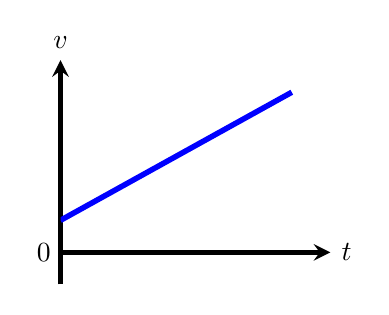
\begin{tikzpicture}  
				\begin{axis}[  ultra thick,scale=0.5,
					xmin=0,  
					xmax=7,  
					ymin=-1,  
					ymax=6, 
					samples=300,
					yticklabels=\empty,
					xticklabels=\empty,
					xtick=\empty,
					ytick=\empty,
					axis lines=center, 
					xlabel=$t$, 		ylabel=$v$,
					every axis y label/.style={at=(current axis.above origin),anchor=south},  
					every axis x label/.style={at=(current axis.right of origin),anchor=west},  ]
					\addplot [line width=2pt, blue, smooth, domain=0:6] {1+2*x/3};  
					\coordinate (O) at (axis cs: 0,0);
				\end{axis}  
				\node[left] at (O) {0};
			\end{tikzpicture}
			&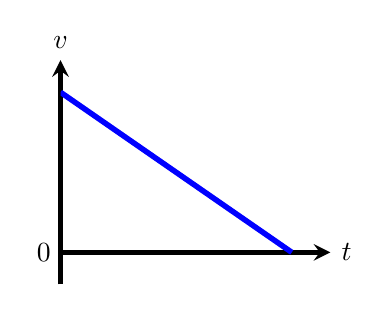
\begin{tikzpicture}  
				\begin{axis}[  ultra thick,scale=0.5,
					xmin=0,  
					xmax=7,  
					ymin=-1,  
					ymax=6, 
					samples=300,
					yticklabels=\empty,
					xticklabels=\empty,
					xtick=\empty,
					ytick=\empty,
					axis lines=center, 
					xlabel=$t$, 		ylabel=$v$,
					every axis y label/.style={at=(current axis.above origin),anchor=south},  
					every axis x label/.style={at=(current axis.right of origin),anchor=west},  ]
					\addplot [line width=2pt, blue, smooth, domain=0:6] {5-5*x/6};  
					\coordinate (O) at (axis cs: 0,0);
				\end{axis}  
				\node[left] at (O) {0};
			\end{tikzpicture}
			&
			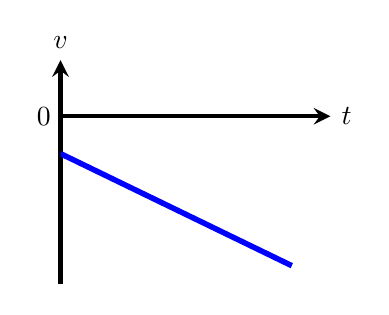
\begin{tikzpicture}  
				\begin{axis}[  ultra thick,scale=0.5,
					xmin=0,  
					xmax=7,  
					ymin=-4.5,  
					ymax=1.5, 
					samples=300,
					yticklabels=\empty,
					xticklabels=\empty,
					xtick=\empty,
					ytick=\empty,
					axis lines=center, 
					xlabel=$t$, 		ylabel=$v$,
					every axis y label/.style={at=(current axis.above origin),anchor=south},  
					every axis x label/.style={at=(current axis.right of origin),anchor=west},  ]
					\addplot [line width=2pt, blue, smooth, domain=0:6] {-1-0.5*x};  
					\coordinate (O) at (axis cs: 0,0);
				\end{axis}  
				\node[left] at (O) {0};
			\end{tikzpicture}
			&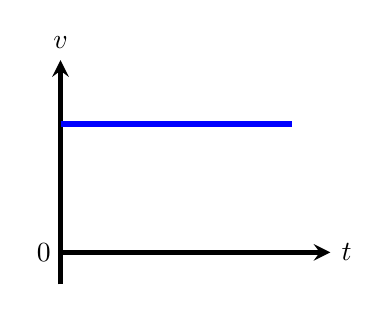
\begin{tikzpicture}  
				\begin{axis}[  ultra thick,scale=0.5,
					xmin=0,  
					xmax=7,  
					ymin=-1,  
					ymax=6, 
					samples=300,
					yticklabels=\empty,
					xticklabels=\empty,
					xtick=\empty,
					ytick=\empty,
					axis lines=center, 
					xlabel=$t$, 		ylabel=$v$,
					every axis y label/.style={at=(current axis.above origin),anchor=south},  
					every axis x label/.style={at=(current axis.right of origin),anchor=west},  ]
					\addplot [line width=2pt, blue, smooth, domain=0:6] {4};  
					\coordinate (O) at (axis cs: 0,0);
				\end{axis}  
				\node[left] at (O) {0};
			\end{tikzpicture}\\
			(I)& (II)& (III)&(IV)
		\end{tabular}
	\end{center}	
	\choice
	{(I), (II) và (III)}
	{(I) và (II)}
	{(I), (II) và (IV)}
	{\True (I) và (III)}
	\loigiai{}
\end{ex}
% ===================================================================
\begin{ex}
Một chất điểm chuyển động biến đổi với công thức vận tốc $v=4+3t\ \left(\si{\meter/\second}; \si{\second}\right)$. Nhận định nào sau đây là đúng khi nói về chuyển động của chất điểm?	
	\choice
	{Chất điểm chuyển động nhanh dần đều theo chiều dương với gia tốc $\SI{6}{\meter/\second^2}$}
	{Chất điểm chuyển động chậm dần đều theo chiều dương với gia tốc $\SI{3}{\meter/\second^2}$}
	{Chất điểm chuyển động nhanh dần đều theo chiều dương với gia tốc $\SI{4}{\meter/\second^2}$}
	{\True Chất điểm chuyển động nhanh dần đều theo chiều dương với gia tốc $\SI{3}{\meter/\second^2}$}
	\loigiai{}
\end{ex}
% ===================================================================
\begin{ex}
\immini{
Hình bên là đồ thị độ dịch chuyển - thời gian của ô tô chuyển động thẳng theo một hướng xác định. Tốc độ lớn nhất của ô tô tương ứng với đoạn nào trên đồ thị?
}	
{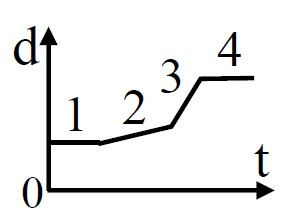
\includegraphics[width=0.35\linewidth]{../figs/D10-2-11}}
	\choice
	{1}
	{2}
	{\True 3}
	{4}
	\loigiai{}
\end{ex}
% ===================================================================
\begin{ex}
	Hình sau thể hiện giờ đi từ Hà Nội (02/01/2024) và giờ đến Vinh của các tàu SE7, SE5, SE3, SE19.
	\begin{center}
		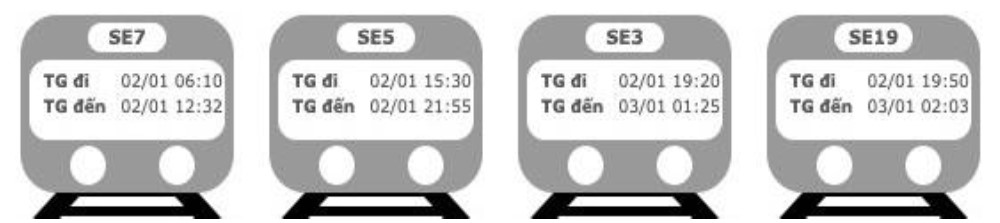
\includegraphics[width=0.7\linewidth]{../figs/D10-2-12}
	\end{center}
	Trong các tàu nói trên, tàu có tốc độ trung bình lớn nhất là
	\choice
	{\True SE3}
	{SE5}
	{SE7}
	{SE19}
	\loigiai{}
\end{ex}
% ===================================================================
\begin{ex}
	Một mặt bàn hình chữ nhật ABCD có chiều dài $\mathrm{AB}=\SI{0.8}{\meter}$ và chiều rộng $\mathrm{BC}=\SI{0.6}{\meter}$. Một con nhện bò dọc theo các cạnh của mặt bàn, từ A đến C. Độ dịch chuyển của con nhện là
	\choice
	{\True $\SI{1.0}{\meter}$}
	{$\SI{1.4}{\meter}$}
	{$\SI{0.2}{\meter}$}
	{$\SI{1.2}{\meter}$}
	\loigiai{}
\end{ex}
% ===================================================================
\begin{ex}
	Một xe xuất phát từ lúc 7 giờ 15 phút sáng từ thành phố M, chuyển động thẳng đều tới thành phố N, cách thành phố M $\SI{90}{\kilo\meter}$. Biết tốc độ của xe là $\SI{60}{\kilo\meter/\hour}$, xe đến thành phố N lúc	
	\choice
	{9 giờ 45 phút}
	{8 giờ 30 phút}
	{9 giờ 30 phút}
	{\True 8 giờ 45 phút}
	\loigiai{
		Thời gian để xe đi từ M đến N:
		$$\Delta t=\dfrac{s}{v}=\SI{1.5}{\hour}.$$
		Thời điểm xe đến N:
		$$t=\SI{7}{\hour}\SI{15}{\minute}+\Delta t=\SI{8}{\hour}\SI{45}{\minute}.$$	
	}
\end{ex}

% ===================================================================
\begin{ex}
Một ô tô chạy trên đoạn đường thẳng từ A đến B mất khoảng thời gian $t$. Trong 1/4 đầu của khoảng thời gian $t$ này, ô tô có tốc độ là $\SI{40}{\kilo\meter/\hour}$. Trong khoảng thời gian còn lại, ô tô có tốc độ là $\SI{60}{\kilo\meter/\hour}$. Tốc độ trung bình của ô tô trên cả đoạn đường AB là	
	\choice
	{$\SI{45}{\kilo\meter/\hour}$}
	{$\SI{49}{\kilo\meter/\hour}$}
	{\True $\SI{55}{\kilo\meter/\hour}$}
	{$\SI{50}{\kilo\meter/\hour}$}
	\loigiai{}
\end{ex}
% ===================================================================
\begin{ex}
	Một chiếc thuyền xuôi dòng từ A đến B với tốc độ $\SI{34}{\kilo\meter/\hour}$ đối với nước. Nước chảy với tốc độ $\SI{2}{\kilo\meter/\hour}$ so với bờ sông. Biết hai bến sông cách nhau $\SI{120}{\kilo\meter}$. Thời gian thuyền đi từ A đến B là
	\choice
	{$\SI{2.94}{\hour}$}
	{$\SI{4.26}{\hour}$}
	{\True $\SI{3.33}{\hour}$}
	{$\SI{2.63}{\hour}$}
	\loigiai{
		Thời gian xuôi dòng:
		$$t_{\text{xd}}=\dfrac{s}{v_t+v_n}\approx\SI{3.33}{\hour}.$$
	}
\end{ex}
% ===================================================================
\begin{ex}
	Một người bơi dọc theo chiều dài $\SI{55}{\meter}$ của bể bơi hết $\SI{50}{\second}$ rồi quay về lại chỗ xuất phát trong $\SI{60}{\second}$. Trong suốt quãng đường đi và về vận tốc trung bình của người đó là
	\choice
	{\True $\SI{0}{\meter/\second}$}
	{$\SI{1.0}{\meter/\second}$}
	{$\SI{1.1}{\meter/\second}$}
	{$\SI{2.0}{\meter/\second}$}
	\loigiai{
		Vì điểm đầu của quĩ đạo chuyển động trùng với điểm cuối nên $d=0\Rightarrow v=0$.	
	}
\end{ex}
% ===================================================================
\begin{ex}
	Xe ô tô đang chuyển động thẳng với vận tốc $\SI{20}{\meter/\second}$ thì hãm phanh chuyển động chậm dần đều. Quãng đường xe đi được từ lúc hãm phanh đến khi xe dừng hẳn là $\SI{100}{\meter}$. Gia tốc của xe là
	\choice
	{$\SI{1}{\meter/\second^2}$}
	{$\SI{5}{\meter/\second^2}$}
	{\True $\SI{-2}{\meter/\second^2}$}
	{$\SI{-1}{\meter/\second^2}$}
	\loigiai{}
\end{ex}
% ===================================================================
\begin{ex}
	Công thức độ dịch chuyển của một vật là $d=-3t+2t^2$ ($x$ tính bằng mét, $t$ tính bằng giây). Công thức vận tốc của vật là
	\choice
	{$v=-3+2t$}
	{\True $v=-3+4t$}
	{$v=-3t+2$}
	{$v=3t$}
	\loigiai{}
\end{ex}
% ===================================================================
\begin{ex}
	Hình bên là đồ thị toạ độ - thời gian của một chiếc xe máy đang chạy trên đường thẳng. Xe này có tốc độ là
	\begin{center}
		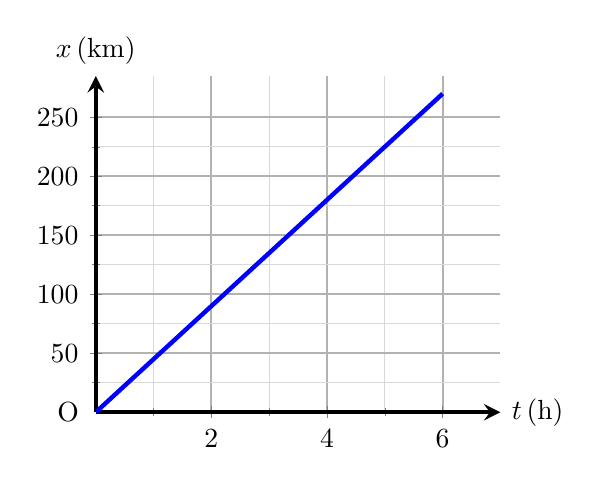
\begin{tikzpicture}  
			\begin{axis}[  ultra thick,scale=0.75,
				xmin=0,  
				xmax=7,  
				xtick={0,2,...,6},
				ytick={0,50,...,250},
				minor x tick num=1,
				minor y tick num=1,
				ymin=0,  
				ymax=285, 
				samples=300,
				axis lines=center, 
				grid style={step=1, line width =0.4pt, color=gray!30!white},
				grid=both, %giới hạn ô lưới
				major grid style={line width=0.8pt,gray!60!white},
				xlabel=$\xsi{t}{\left(\si{\hour}\right)}$, 		ylabel=$\xsi{x}{\left(\si{\kilo\meter}\right)}$,
				every axis y label/.style={at=(current axis.above origin),anchor=south},  
				every axis x label/.style={at=(current axis.right of origin),anchor=west},  ] 
				\addplot [ultra thick, blue, smooth, domain=0:6] {45*x}; 
			\end{axis} 
			\node at (-0.35,0) {O}; 
		\end{tikzpicture}
		
	\end{center}
	\choice
	{\True $\SI{45}{\kilo\meter/\hour}$}
	{$\SI{43.75}{\kilo\meter/\hour}$}
	{$\SI{45.45}{\kilo\meter/\hour}$}
	{$\SI{50}{\kilo\meter/\hour}$}
	\loigiai{
		Tại $t=\SI{5}{\hour}$ thì $x=\SI{225}{\kilo\meter}$:
		$$\left|v\right|=\left|\dfrac{\Delta x}{\Delta t}\right|=\SI{45}{\kilo\meter/\hour}.$$	
	}
\end{ex}

% ===================================================================
\begin{ex}
	Một ô tô đang chạy với tốc độ $\SI{72}{\kilo\meter/\hour}$ thì hãm phanh chuyển động thẳng chậm dần đều với gia tốc có độ lớn $\SI{0.5}{\meter/\second^2}$. Quãng đường mà ô tô đã đi được trong 5 giây cuối trước khi dừng lại là
	\choice
	{$\SI{68.75}{\meter}$}
	{$\SI{81.25}{\meter}$}
	{$\SI{12.5}{\meter}$}
	{\True $\SI{6.25}{\meter}$}
	\loigiai{
		Đảo ngược thời gian sẽ thấy xe chuyển động nhanh dần đều với gia tốc $a=\SI{0.5}{\meter/\second^2}$, không vận tốc đầu. Lúc này, 5 giây cuối trở thành 5 giây đầu:
		$$s=\dfrac{1}{2}at^2=\dfrac{1}{2}\cdot0,5\cdot5^2=\SI{6.25}{\meter}.$$
	}
\end{ex}

\Closesolutionfile{ans}
\section{Câu trắc nghiệm đúng/sai} 
\textit{Thí sinh trả lời từ câu 1 đến câu 2. Trong mỗi ý \textbf{a)}, \textbf{b)}, \textbf{c)}, \textbf{d)} ở mỗi câu, thí sinh chọn đúng hoặc sai}
\setcounter{ex}{0}
\Opensolutionfile{ans}[ans/D10-GKI-002-TF]
\begin{ex}
	Một vật chuyển động thẳng có đồ thị vận tốc theo thời gian như hình bên dưới.
	\begin{center}
		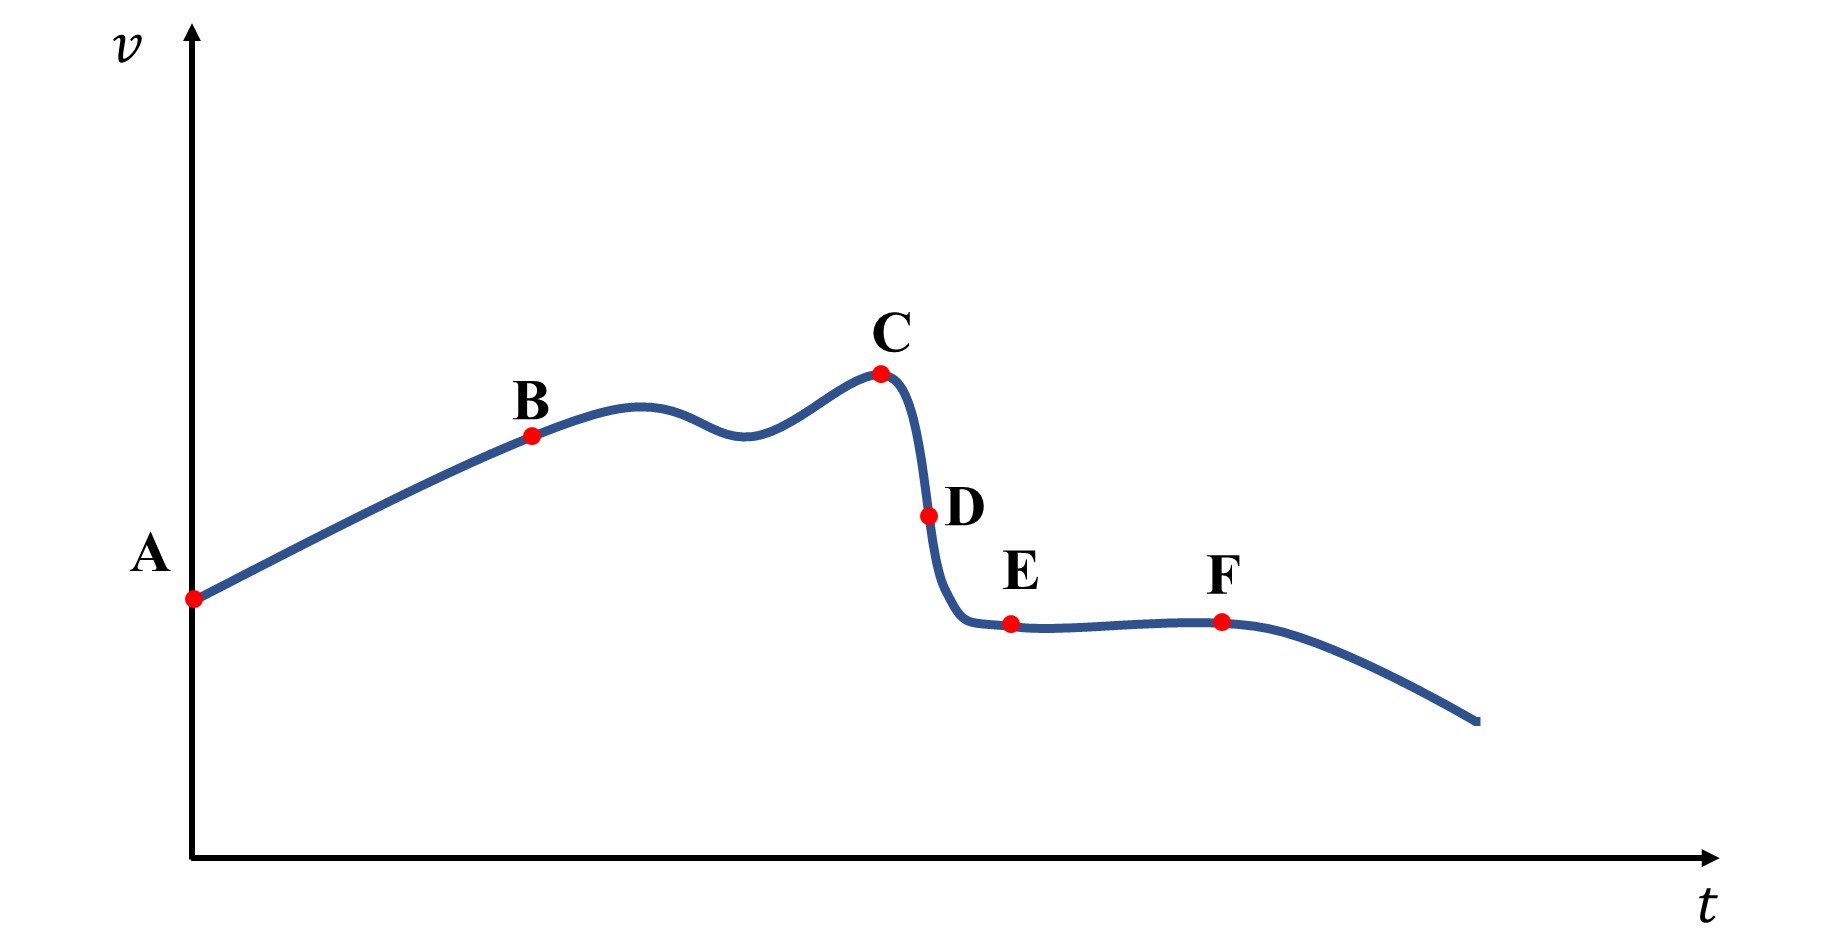
\includegraphics[width=0.7\linewidth]{../figs/D10-2-8}
	\end{center}
	\choiceTF[t]
	{Vật đạt tốc độ lớn nhất tại B}
	{Trong quá trình AB, vật chuyển động thẳng đều}
	{Trong quá trình EF, vật đứng yên}
	{\True Độ lớn gia tốc tại D lớn hơn độ lớn gia tốc tại B}
	\loigiai{}
\end{ex}

% ===================================================================
\begin{ex}
	Một thiết bị tạo ra các chấm trên một băng giấy chuyển động với khoảng thời gian giữa 2 chấm liên tiếp là $\SI{0.02}{\second}$. Hình 1, Hình 2 và Hình 3 biểu diễn kết 3 quả chuyển động thẳng của băng giấy. Mốc thời gian được chọn tại chấm 0.
	\begin{center}
		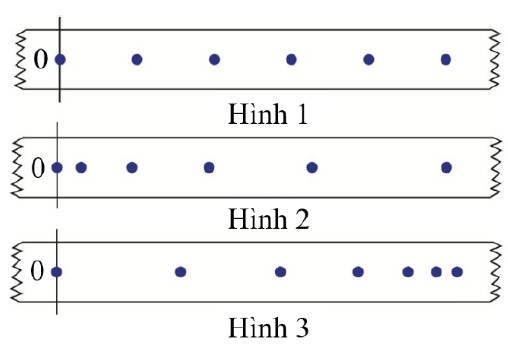
\includegraphics[width=0.4\linewidth]{../figs/D10-2-9}
	\end{center}
	\choiceTF[t]
	{\True Kết quả ở Hình 1 chứng tỏ băng giấy chuyển động thẳng đều}
	{Kết quả ở Hình 2 và Hình 3 chứng tỏ băng giấy chuyển động nhanh dần}
	{\True Tốc độ trung bình của băng giấy ở Hình 1 và Hình 2 trong $\SI{0.1}{\second}$ (tính từ mốc thời gian) là bằng nhau}
	{Độ lớn gia tốc của băng giấy ở Hình 2 lớn hơn độ lớn gia tốc của băng giấy ở Hình 3}
	\loigiai{
	\begin{itemchoice}
		\itemch Đúng.
		\itemch Sai. Hình 2 băng giấy chuyển động nhanh dần, Hình 3 băng giấy chuyển động chậm dần.
		\itemch Đúng.
		\itemch Sai. Chưa thể khẳng định vật chuyển động biến đổi đều nên chưa thể so sánh gia tốc trong 2 trường hợp.
	\end{itemchoice}
	}
\end{ex}
\Closesolutionfile{ans}
\section{Câu trắc nghiệm trả lời ngắn} \textit{Thí sinh trả lời từ câu 1 đến câu 6}
\setcounter{ex}{0}
\Opensolutionfile{ans}[ans/D10-GKI-002-TL]
% ===============================================================
\begin{ex}
	\immini{
	Chuyển động của một viên bi có đồ thị vận tốc - thời gian như hình bên. Ở thời điểm nào (tính bằng giây), vận tốc viên bi có giá trị bằng không?
	}
	{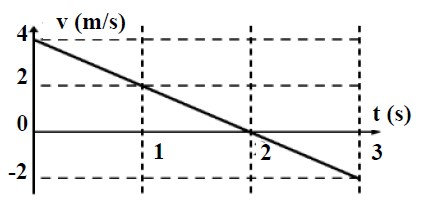
\includegraphics[width=0.55\linewidth]{../figs/D10-2-13}}
	\shortans{2 }
	\loigiai{
		
	}
\end{ex}
% ===================================================================
\begin{ex}
	Một con bọ rùa bò đều trên các cạnh của một tấm ván hình chữ nhật với chiều dài các cạnh $\mathrm{AB}=\SI{40}{\centi\meter}$, $\mathrm{BC}=\SI{20}{\centi\meter}$, mỗi 2 giây nó bò được $\SI{1.5}{\centi\meter}$. Tại thời điểm ban đầu, con bọ rùa ở đỉnh A của tấm ván. Kể từ thời điểm ban đầu, trong thời gian $\SI{80}{\second}$, vận tốc trung bình là bao nhiêu $\si{\centi\meter/\second}$? \textit{(Kết quả làm tròn đến 2 chữ số sau dấu thập phân.)}
	\shortans{$0,56$}
	\loigiai{
		Trong $\SI{80}{\second}$ con bọ rùa bò được $\SI{60}{\centi\meter}$ nên đi được hết cạnh AC và BC.\\
		$$v=\dfrac{\sqrt{\mathrm{AC}^2+\mathrm{BC}^2}}{t}\approx\SI{0.56}{\centi\meter/\second}.$$
	}
\end{ex}
% ===================================================================
\begin{ex}
	Chuyển động của hai viên bi $\mathrm{B}_1$ và $\mathrm{B}_2$ có đồ thị vận tốc thời gian như hình bên. Gọi $s_1$ và $s_2$ là quãng đường đi được tương ứng của $\mathrm{B}_1$ và $\mathrm{B}_2$ trong cùng thời gian kể từ thời điểm $t=\SI{0}{\second}$. Tỉ số $s_2/s_1$ là bao nhiêu? \textit{(Kết quả lấy đến 1 chữ số sau dấu phẩy thập phân)}.
	\begin{center}
		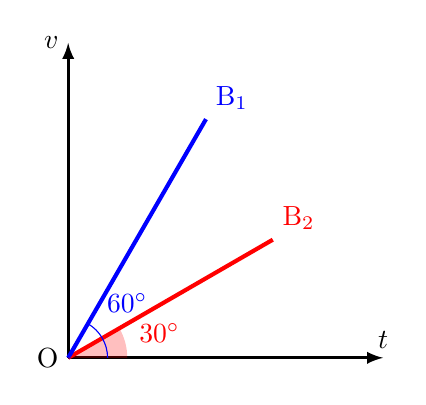
\begin{tikzpicture} 
			\coordinate (O)  at (0,0);
			\coordinate (t) at (4,0);
			\coordinate (v) at (0,4);
			\coordinate (A) at ($(O)+(30:3)$);
			\coordinate (B) at ($(O)+(60:3.5)$);
			\draw[line width=1pt, -latex] (O)--(v);
			\draw[line width=1pt, -latex] (O)--(t);
			\draw[line width=1.5pt, red] (O)--(A);
			\draw[line width=1.5pt, blue] (O)--(B);
			\node[left] at (O) {O};
			\node[above] at (t) {$t$};
			\node[left] at (v) {$v$};
			\tkzFillAngle[size=0.75cm,color=red, fill=red, opacity=0.25](t,O,A);
			\tkzLabelAngle[color=red,pos=1.2](t,O,A){$\SI{30}{\degree}$}
			\tkzMarkAngle[size=0.5cm,color=blue](t,O,B);
			\node[blue] at (0.75,0.7) {$\SI{60}{\degree}$};
			\node[above right, red] at (A) {$\mathrm{B}_2$};
			\node[above right, blue] at (B) {$\mathrm{B}_1$};
		\end{tikzpicture}
	\end{center}
	\shortans{0,3}
	\loigiai{
	$$\dfrac{s_2}{s_1}=\dfrac{\dfrac{1}{2}a_2t^2}{\dfrac{1}{2}a_1t^2}=\dfrac{a_2}{a_1}=\dfrac{\tan\SI{30}{\degree}}{\tan\SI{60}{\degree}}\approx0,3.$$
	}
\end{ex}
% ===============================================================
\begin{ex}
	Hình bên dưới mô tả vị trí của xe ô tô trong khoảng thời gian $\SI{5}{\second}$ kể từ lúc xe bắt đầu tăng tốc đều từ trạng thái nghỉ. Sau $\SI{6}{\second}$ xe cách vị trí ban đầu bao nhiêu mét?
	\begin{center}
		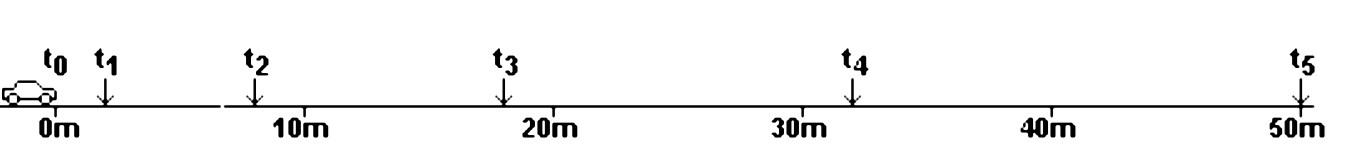
\includegraphics[width=0.8\linewidth]{../figs/D10-2-14}
	\end{center}
	\shortans{72}
	\loigiai{
		
	}
\end{ex}
% ===============================================================
\begin{ex}
Trên quãng đường AB có hai xe chuyển động thẳng. Xe 1 đi từ A tới B với tốc độ trung bình $\SI{32}{\kilo\meter/\hour}$. Xe 2 đi từ B đến A, nửa quãng đường đầu chuyển động đều với tốc độ $\SI{60}{\kilo\meter/\hour}$, nửa quãng đường sau chuyển động đều với tốc độ $\SI{40}{\kilo\meter/\hour}$. Hai xe đến đích cùng lúc, xe 1 xuất phát sớm hơn xe 2 một khoảng thời gian 1 giờ. Tính quãng đường AB theo đơn vị kilomet?
	\shortans{96 }
	\loigiai{
		
	}
\end{ex}
% ===============================================================
\begin{ex}
	Hai chất điểm chuyển động trên hai trục tọa độ vuông góc $Ox$, $Oy$ và đi qua $O$ cùng lúc. Vật thứ nhất chuyển động trên trục $Ox$ theo chiều dương với gia tốc không đổi bằng $\SI{1}{\meter/\second^2}$ và tốc độ khi đi qua O là $\SI{6}{\meter/\second}$. Vật thứ hai chuyển động chậm dần đều theo chiều âm trên trục $Oy$ với gia tốc có độ lớn $\SI{2}{\meter/\second^2}$ và  tốc độ khi đi qua O là $\SI{8}{\meter/\second}$. Độ lớn vận tốc nhỏ nhất của vật thứ nhất đối với vật thứ hai trong khoảng thời gian kể từ lúc đi qua O cho đến khi vật thứ hai dừng là bao nhiêu $\si{\meter/\second}$? \textit{(Kết quả làm tròn đến 2 chữ số sau dấu phẩy thập phân)}.
	\shortans{$8,94$ }
	\loigiai{
		
	}
\end{ex}
\Closesolutionfile{ans}
\begin{center}
	\textbf{-- HẾT --}
\end{center}
%	\begin{center}
	\begin{tabular}{M{9.25cm}M{8.75cm}}
		\textbf{TRƯỜNG THCS-THPT NGUYỄN KHUYẾN}& \textbf{ÔN TẬP GIỮA HỌC KÌ 1}\\
		\textbf{MÃ ĐỀ: 001}& \textbf{Bài thi môn: VẬT LÝ 10}\\
		\textit{(Đề thi có 06 trang)}& \textit{Thời gian làm bài: 45 phút, không kể phát đề}
		
		\noindent\rule{4cm}{0.8pt} \\
	\end{tabular}
\end{center}
\setcounter{section}{0}
\begin{center}
	\textbf{\large BẢNG ĐÁP ÁN}
\end{center}
\section{}
\inputansbox{10}{ans/D10-GKI-001-TN}
\section{}
\inputansbox[2]{2}{ans/D10-GKI-001-TF}
\section{}
\inputansbox[3]{6}{ans/D10-GKI-001-TL}\newpage
% =============== ÔN TẬP KIỂM TRA THƯỜNG XUYÊN 2
%\begin{center}
	\begin{tabular}{M{9.25cm}M{8.75cm}}
		\textbf{TRƯỜNG THCS-THPT NGUYỄN KHUYẾN}& \textbf{ÔN TẬP KTTX LẦN 2 HỌC KÌ I}\\
		\textbf{MÃ ĐỀ: 001}& \textbf{Bài thi môn: VẬT LÝ 10}\\
		\textit{(Đề thi có 05 trang)}& \textit{Thời gian làm bài: 40 phút, không kể phát đề}
		
		\noindent\rule{4cm}{0.8pt} \\
	\end{tabular}
\end{center}
\setcounter{section}{0}
\section{Câu trắc nghiệm nhiều phương án lựa chọn}
\textit{Thí sinh trả lời từ câu 1 đến câu 20. Mỗi câu hỏi thí sinh chọn một phương án}
\setcounter{ex}{0}
\Opensolutionfile{ans}[ans/D10-HKI-KTTX2-001-TN]
% ===================================================================
\begin{ex}
	Đơn vị đo lực (newton) được viết theo các đơn vị cơ bản trong hệ SI là
	\choice
	{$\si{\kilogram/\meter^2}$}
	{$\si{\kilogram/\second^2}$}
	{$\si{\kilogram\cdot\meter^2/\second}$}
	{\True $\si{\kilogram\cdot\meter/\second^2}$}
	\loigiai{}
\end{ex}
% ===================================================================
\begin{ex}
	Phát biểu nào sau đây là đúng?
	\choice
	{\True Khi vận tốc của vật thay đổi thì chắc chắn đã có lực tác dụng lên vật}
	{Nếu không chịu lực nào tác dụng thì vật phải đứng yên}
	{Khi không chịu lực nào tác dụng lên vật thì vật đang chuyển động sẽ lập tức dừng lại}
	{Vật chuyển động được là nhờ có lực tác dụng lên nó}
	\loigiai{}
\end{ex}
% ===================================================================
\begin{ex}
	Nhận định nào dưới đây về lực là \textbf{chính xác nhất}?\\
	Lực là đại lượng đặc trưng cho tác dụng của vật này lên vật khác. Dưới tác dụng của lực
	\choice
	{vật sẽ chuyển động thẳng đều hoặc quay tròn đều}
	{vật sẽ thu gia tốc và chuyển động biến đổi}
	{vật sẽ bị biến dạng}
	{\True vật sẽ thay đổi trạng thái chuyển động hoặc biến dạng}
	\loigiai{}
\end{ex}

% ===================================================================
\begin{ex}
	Trong chuyển động thẳng chậm dần đều thì hợp lực tác dụng vào vật
	\choice
	{\True ngược chiều chuyển động và có độ lớn không đổi và khác không}
	{cùng chiều chuyển động và có độ lớn giảm dần}
	{ngược chiều chuyển động và có độ lớn giảm dần}
	{cùng chiều chuyển động và có độ lớn không đổi và khác không}
	\loigiai{}
\end{ex}
% ===================================================================
\begin{ex}
	Phát biểu nào sau đây là đúng?
	\choice
	{Vật luôn luôn chuyển động cùng chiều với hợp lực tác dụng lên nó}
	{\True Gia tốc của vật luôn cùng chiều với hợp lực tác dụng lên nó}
	{Hợp lực tác dụng lên vật giảm dần thì vật chuyển động chậm dần}
	{Hợp lực tác dụng lên vật không đổi thì vật chuyển động thẳng đều}
	\loigiai{}
\end{ex}
% ===================================================================
\begin{ex}
	Một vật đang chuyển động với vận tốc $v$. Nếu bỗng nhiên các lực tác dụng lên nó mất đi thì vật
	\choice
	{chuyển động chậm dần rồi dừng lại}
	{đổi hướng chuyển động}
	{\True chuyển động thẳng đều}
	{dừng lại ngay}
	\loigiai{}
\end{ex}
% ===================================================================
\begin{ex}
	Nhìn chiếc xe tải chạy trên đoạn đường thẳng nằm ngang với vận tốc không đổi, ta có thể tin rằng
	\choice
	{người lái xe đã cho động cơ ngừng hoạt động và xe tiếp tục chạy theo quán tính}
	{trên xe không có hàng hóa, ma sát xuất hiện là rất bé và không làm thay đổi vận tốc của xe}
	{\True lực tác dụng của động cơ làm cho xe chuyển động cân bằng với tất cả các lực cản tác dụng lên xe}
	{hợp lực của lực động cơ và mọi lực cản là một lực không đổi và cùng hướng chuyển động của xe}
	\loigiai{}
\end{ex}
% ===================================================================
\begin{ex}
Cho hai lực $\vec{F}_1$ và $\vec{F}_2$ đồng quy. Hai lực phải thỏa điều kiện nào sau đây để độ lớn hợp của hai lực bằng 0?
	\choice
	{Hai lực có độ lớn bằng nhau}
	{Hai lực song song, ngược chiều}
	{\True Hai lực song song, ngược chiều và có độ lớn bằng nhau}
	{Hai lực song song, cùng chiều và có độ lớn bằng nhau}
	\loigiai{}
\end{ex}
% ===================================================================
\begin{ex}
	Một vật đang chuyển động dưới tác dụng của lực không đổi $\vec{F}_1$ với gia tốc $a_1$. Nếu tăng độ lớn lực tác dụng thành $F_2=2F_1$ thì gia tốc của vật là $a_2$. Mối liên hệ giữa $a_2$ và $a_1$ là
	\choice
	{$a_1=2a_2$}
	{$a_2=a_1$}
	{\True $a_2=2a_1$}
	{$a_2=4a_1$}
	\loigiai{}
\end{ex}

% ===================================================================
\begin{ex}
	\immini{Con chó săn to khỏe và chạy nhanh hơn thỏ. Tuy nhiên khi thỏ bị chó săn rượt đuổi, thỏ vẫn có thể thoát nạn nhờ vận dụng chiến thuật luôn luôn đổi hướng chạy đột ngột làm chó săn lỡ đà. Điều này dựa vào tính chất nào trong vật lý?}{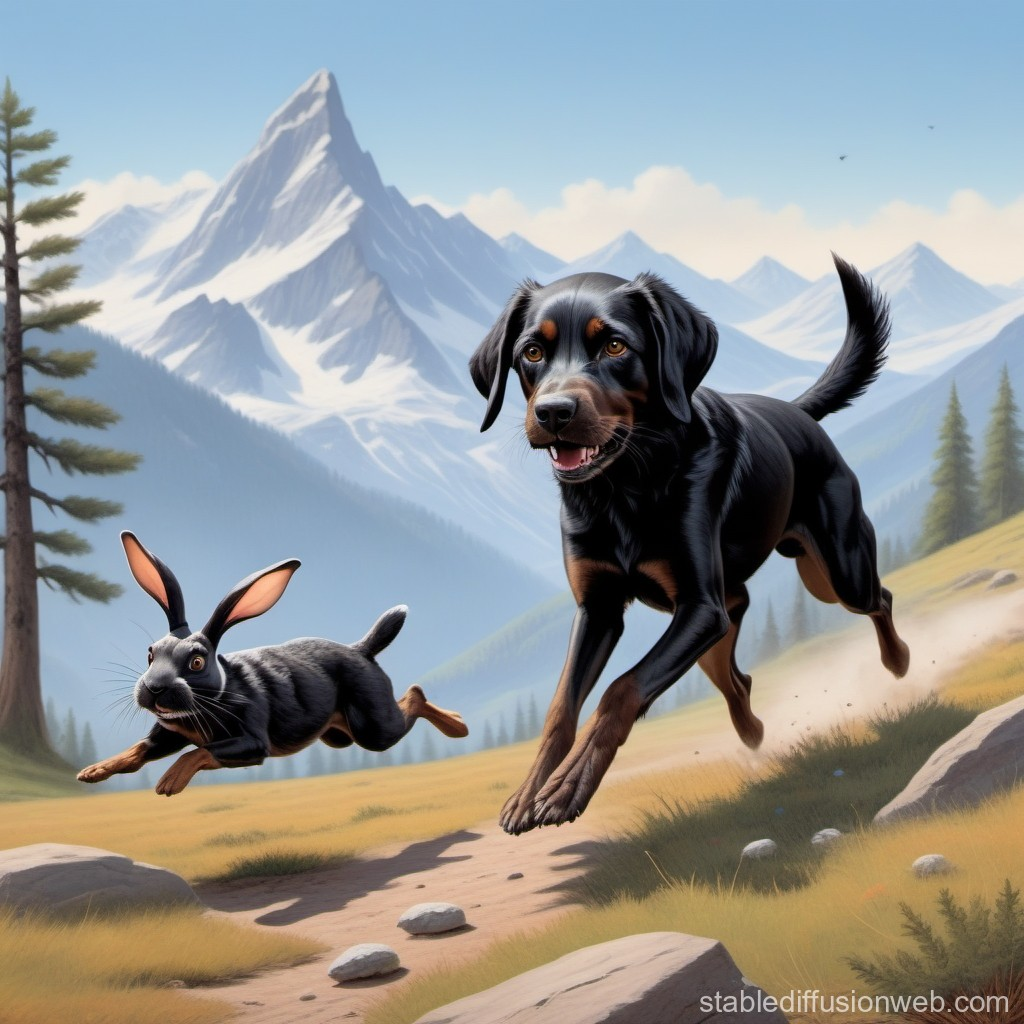
\includegraphics[width=0.4\linewidth]{../figs/D10-HKI-KTTX2-001-1}}
	\choice
	{Trọng lượng}
	{Lực}
	{\True Quán tính}
	{Vận tốc}
	\loigiai{}
\end{ex}
% ===================================================================
\begin{ex}
Một chất điểm chịu tác dụng của một lực $\vec{F}$ có độ lớn $\SI{20}{\newton}$. Nếu hai lực thành phần của lực đó vuông góc với nhau	và có độ lớn lần lượt là $F_1=\SI{12}{\newton}$ và $F_2$ thì $F_2$ bằng
	\choice
	{\True $\SI{8}{\newton}$}
	{$\SI{16}{\newton}$}
	{$\SI{32}{\newton}$}
	{$\SI{20}{\newton}$}
	\loigiai{}
\end{ex}
% ===================================================================
\begin{ex}
Hai lực khác phương $\vec{F}_1$ và $\vec{F}_2$ có độ lớn $F_1=F_2=\SI{20}{\newton}$, góc tạo bởi hai lực này là $\SI{60}{\degree}$. Hợp lực của hai lực này có độ lớn là	
	\choice
	{$\SI{14.1}{\newton}$}
	{\True $\xsi{20\sqrt{3}}{\newton}$}
	{$\SI{17.3}{\newton}$}
	{$\SI{20}{\newton}$}
	\loigiai{}
\end{ex}
% ===================================================================
\begin{ex}
	Một chất điểm đứng yên dưới tác dụng của 3 lực có giá đồng quy và có độ lớn lần lượt là $\SI{8}{\newton}$, $\SI{10}{\newton}$, $\SI{12}{\newton}$. Nếu bỏ đi lực $\SI{10}{\newton}$ thì hợp lực của hai lực còn lại là
	\choice
	{$\SI{20}{\newton}$}
	{$\SI{6}{\newton}$}
	{$\SI{4}{\newton}$}
	{\True $\SI{10}{\newton}$}
	\loigiai{}
\end{ex}
% ===================================================================
\begin{ex}
	Hai vật có cùng khối lượng bắt đầu chuyển động dưới tác dụng của hai lực cùng phương, cùng chiều và có độ lớn $F_1>F_2$. Quãng đường $s_1$, $s_2$ mà hai vật đi được trong cùng một khoảng thời gian sẽ thỏa
	\choice
	{$\dfrac{s_1}{s_2}=\dfrac{F_2}{F_1}$}
	{\True $\dfrac{s_1}{s_2}=\dfrac{F_1}{F_2}$}
	{$\dfrac{s_1}{s_2}>\dfrac{F_2}{F_1}$}
	{$\dfrac{s_1}{s_2}<\dfrac{F_2}{F_1}$}
	\loigiai{}
\end{ex}
% ===================================================================
\begin{ex}
Sau thời gian $\SI{0.02}{\second}$ tiếp xúc với chân của cầu thủ, quả bóng khối lượng $\SI{500}{\gram}$ ban đầu đứng yên sẽ bay đi với tốc độ $\SI{54}{\kilo\meter/\hour}$. Lực tác dụng lên quả bóng có độ lớn là	
	\choice
	{$\SI{250}{\newton}$}
	{\True $\SI{375}{\newton}$}
	{$\SI{1.35}{\kilo\newton}$}
	{$\SI{13.5}{\kilo\newton}$}
	\loigiai{}
\end{ex}
% ===================================================================
\begin{ex}
	Cho hai lực đồng quy có độ lớn bằng $\SI{8}{\newton}$ và $\SI{12}{\newton}$. Giá trị của hợp lực \textbf{không thể} nhận giá trị nào trong các giá trị sau đây?
	\choice
	{$\SI{7}{\newton}$}
	{$\SI{19}{\newton}$}
	{$\SI{4}{\newton}$}
	{\True $\SI{21}{\newton}$}
	\loigiai{}
\end{ex}
% ===================================================================
\begin{ex}
	Cho hai lực đồng qui có cùng độ lớn $\SI{600}{\newton}$. Nếu hợp lực của hai lực cũng có độ lớn bằng $\SI{600}{\newton}$ thì góc giữa 2 lực bằng
	\choice
	{$\SI{0}{\degree}$}
	{$\SI{180}{\degree}$}
	{$\SI{60}{\degree}$}
	{\True $\SI{120}{\degree}$}
	\loigiai{}
\end{ex}
% ===================================================================
\begin{ex}
	Một chất điểm đứng yên dưới tác dụng của 3 lực có độ lớn bằng nhau. Kết luận nào sau đây là đúng?
	\choice
	{Có 2 lực cùng giá, ngược chiều nhau}
	{Ba lực có giá cùng nằm trong một mặt phẳng, trong đó 2 lực có giá vuông góc nhau}
	{\True Ba lực có giá cùng nằm trong một mặt phẳng và đôi một hợp nhau góc $\SI{120}{\degree}$}
	{Có 2 lực cùng giá, cùng chiều nhau}
	\loigiai{}
\end{ex}
% ===================================================================
\begin{ex}
	Một vật nhỏ có khối lượng $\SI{2}{\kilogram}$, lúc đầu đứng yên. Nó bắt đầu chịu tác dụng đồng thời của hai lực $F_1=\SI{4}{\newton}$ và $F_2=\SI{3}{\newton}$. Góc giữa $\vec{F}_1$ và $\vec{F}_2$ bằng $\SI{30}{\degree}$. Quãng đường vật đi được sau $\SI{1.2}{\second}$ \textbf{gần nhất} với giá trị nào?
	\choice
	{$\SI{2}{\meter}$}
	{\True $\SI{2.45}{\meter}$}
	{$\SI{2.88}{\meter}$}
	{$\SI{3.16}{\meter}$}
	\loigiai{}
\end{ex}
% ===================================================================
\begin{ex}
	Một lực $\vec{F}$ không đổi truyền cho một vật có khối lượng $m_1$ một gia tốc bằng $\SI{4}{\meter/\second^2}$, truyền cho một vật khác có khối lượng $m_2$ một gia tốc bằng $\SI{2}{\meter/\second^2}$. Nếu đem ghép hai vật đó làm một vật thì lực $\vec{F}$ truyền cho vật ghép một gia tốc có độ lớn là
	\choice
	{$\SI{1.03}{\meter/\second^2}$}
	{\True $\SI{1.33}{\meter/\second^2}$}
	{$\SI{3.33}{\meter/\second^2}$}
	{$\SI{3.03}{\meter/\second^2}$}
	\loigiai{}
\end{ex}
\Closesolutionfile{ans}
\section{Câu trắc nghiệm đúng/sai} 
\textit{Thí sinh trả lời từ câu 1 đến câu 2. Trong mỗi ý \textbf{a)}, \textbf{b)}, \textbf{c)}, \textbf{d)} ở mỗi câu, thí sinh chọn đúng hoặc sai}
\setcounter{ex}{0}\\
\Opensolutionfile{ans}[ans/D10-HKI-KTTX2-001-TF]
% ===================================================================
\begin{ex}
	Một bạn học sinh có khối lượng $m=\SI{55}{\kilogram}$ đang thực hiện động tác bật nhảy tại chỗ (jump squat) bằng hai chân trên sàn cứng như hình minh họa bên dưới.
	\begin{center}
		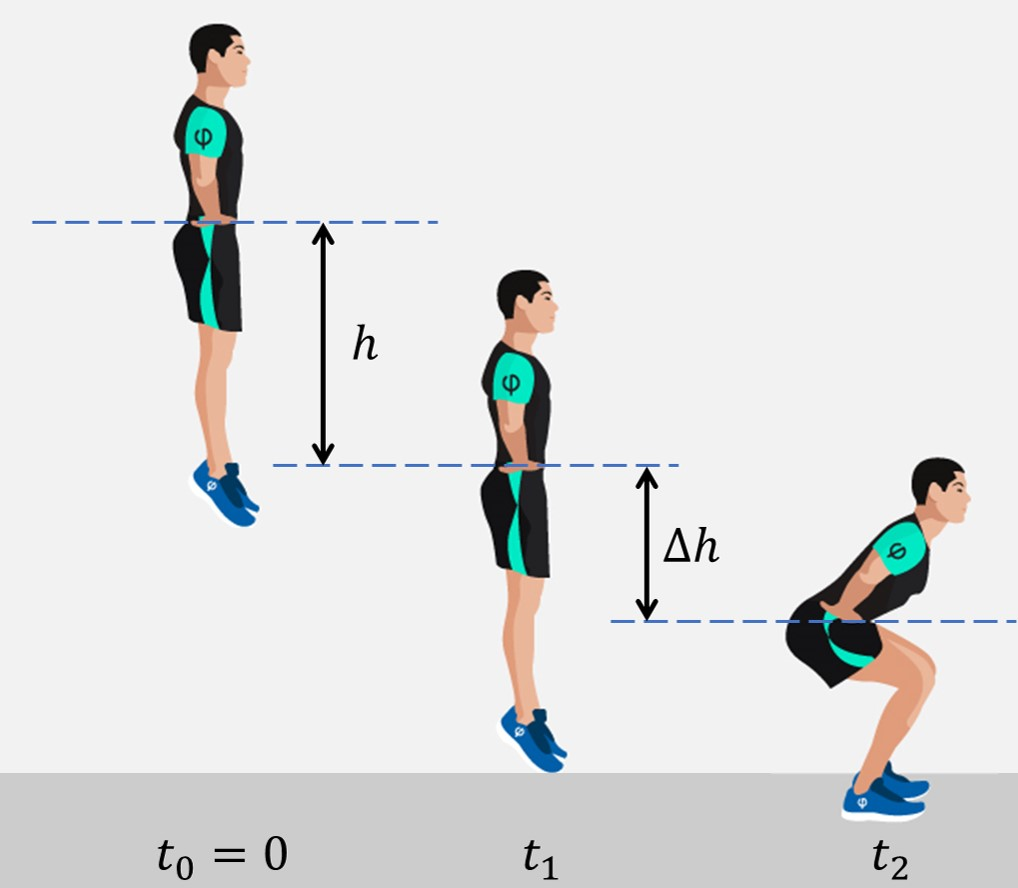
\includegraphics[width=0.4\linewidth]{figs/D10-HKI-KTTX2-001-5}
	\end{center} 
	Tại thời điểm $t_0=0$, học sinh đạt độ cao cực đại và vận tốc bằng 0. Tại thời điểm $t_1$, học sinh này rơi xuống chạm vào mặt sàn bằng hai chân, trọng tâm thân người di chuyển đoạn $h=\SI{0.65}{\meter}$ so với trọng tâm tại thời điểm $t_0$. Để giảm lực tác động lên khớp gối và cột sống trong quá trình tiếp xúc với sàn, bạn này thực hiện động tác gập gối sao cho giữa các thời điểm $t_1$ và $t_2$ trọng tâm của bạn ấy hạ xuống một khoảng $\Delta h=\SI{0.36}{\meter}$.  Trong quá trình rơi trước khi tiếp đất, học sinh rơi nhanh dần đều với gia tốc trọng trường $g=\SI{10}{\meter/\second^2}$ và trọng lực tác dụng lên bạn học sinh được xác định bởi $\vec{P}=m\vec{g}$.
	\choiceTF[t]
	{\True Tốc độ của bạn học sinh ngay trước khi chạm đất là $\SI{3.6}{\meter/\second}$}
	{\True Gia tốc trung bình của bạn học sinh trong quá trình tiếp đất có độ lớn là $\SI{18}{\meter/\second^2}$}
	{Độ lớn lực cản trung bình do sàn tác dụng lên người trong quá trình tiếp đất là $\SI{990}{\newton}$}
	{\True Thời gian mà bạn học sinh tiếp đất là $\SI{0.2}{\second}$}
	\loigiai{
	\begin{itemchoice}
		\itemch Đúng. $v=\sqrt{2gh}\approx\SI{3.6}{\meter/\second}$.
		\itemch Đúng. $a=\dfrac{-v^2}{2\Delta h}\approx\SI{18}{\meter/\second^2}$.
		\itemch  Sai. $F_c=m\left(g+\left|a\right|\right)\approx\SI{1540}{\newton}$.
		\itemch Đúng. $\Delta t=\dfrac{-v}{a}\approx\SI{0.2}{\second}$.
	\end{itemchoice}
	}
\end{ex}
% ===================================================================
\begin{ex}
	Một người dùng đòn gánh dài $\SI{1.8}{\meter}$ để gánh hai vật $m_1=\SI{20}{\kilogram}$ và $m_2=\SI{25}{\kilogram}$ như hình vẽ. 
	\begin{center}
		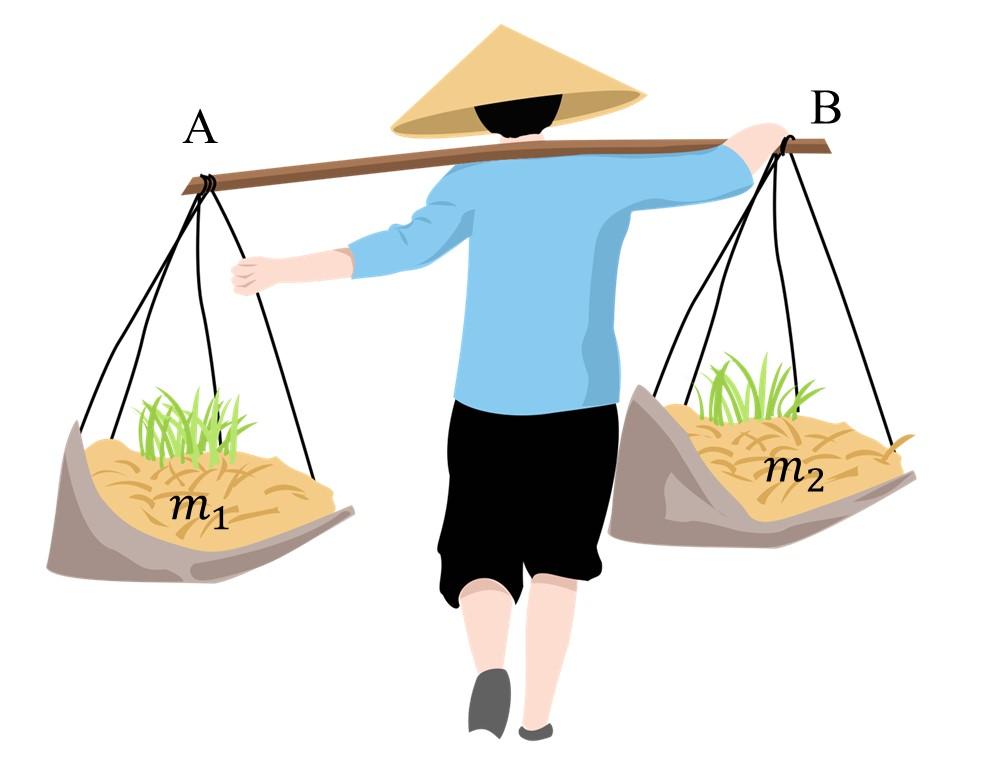
\includegraphics[width=0.3\linewidth]{figs/D10-HKI-KTTX2-001-3}
	\end{center}
	Biết điểm treo hai quang gánh được đặt sát hai đầu đòn gánh, bỏ qua khối lượng của đòn gánh.  Lấy trọng lượng bằng 10 lần khối lượng $P=10m$.
	\choiceTF[t]
	{Trọng lực của vật $m_1$ tác dụng lên đầu A và trọng lực của vật $m_2$ tác dụng lên đầu B là như nhau}
	{\True Điểm đặt vai của người chịu tác dụng của hai lực song song cùng chiều}
	{Để đòn gánh nằm ngang thì vai người đặt ở vị trí chính giữa của đòn gánh}
	{\True Khi gánh nằm ngang thì lực đòn gánh tác dụng lên vai là $\SI{450}{\newton}$ và vai cách đầu A đoạn $\SI{1}{\meter}$}
	\loigiai{
		\begin{itemchoice}
			\itemch Sai. $P_1=\SI{200}{\newton}$; $P_2=\SI{250}{\newton}$.
			\itemch Đúng.
			\itemch Sai. $\dfrac{d_2}{d_1}=\dfrac{P_1}{P_2}=\dfrac{4}{5}$ mà $d_1+d_2=\SI{1.8}{\meter}\Rightarrow \begin{cases}
				d_1=\SI{1}{\meter}\\
				d_2=\SI{0.8}{\meter}
			\end{cases}$.
			\itemch Đúng.
		\end{itemchoice}
	}
\end{ex}
\Closesolutionfile{ans}
\section{Câu trắc nghiệm trả lời ngắn} \textit{Thí sinh trả lời từ câu 1 đến câu 6}
\setcounter{ex}{0}
\Opensolutionfile{ans}[ans/D10-HKI-KTTX2-001-TL]
% ===============================================================
\begin{ex}
	Siêu xe Pininfarina Battista sản xuất tại Italy, được trang bị khả năng động học nâng cao nhờ gói khí động học riêng biệt, có khối lượng khoảng $\SI{2000}{\kilogram}$ đang là siêu xe tăng tốc nhanh nhất thế giới khi chỉ cần 2 giây để tăng tốc từ 0 đến $\SI{28}{\meter/\second}$. Lực để tạo ra gia tốc cho xe trong trường hợp này là bao nhiêu kilo newton $\left(\si{\kilo\newton}\right)$?
	\shortans[oly]{28}
	\loigiai{
		
	}
\end{ex}
% ===============================================================
\begin{ex}
	\immini{Một nha sĩ dùng dây cung niềng răng để chỉnh hình răng khểnh cho một bệnh nhân như hình bên. Lực căng của mỗi dây được điều chỉnh để có độ lớn $\SI{18.0}{\newton}$. Tìm độ lớn của hợp lực do sợi dây tác dụng lên chiếc răng theo đơn vị newton $\left(\si{\newton}\right)$. \textit{(Kết quả làm tròn đến chữ số hàng phần mười)}.}
	{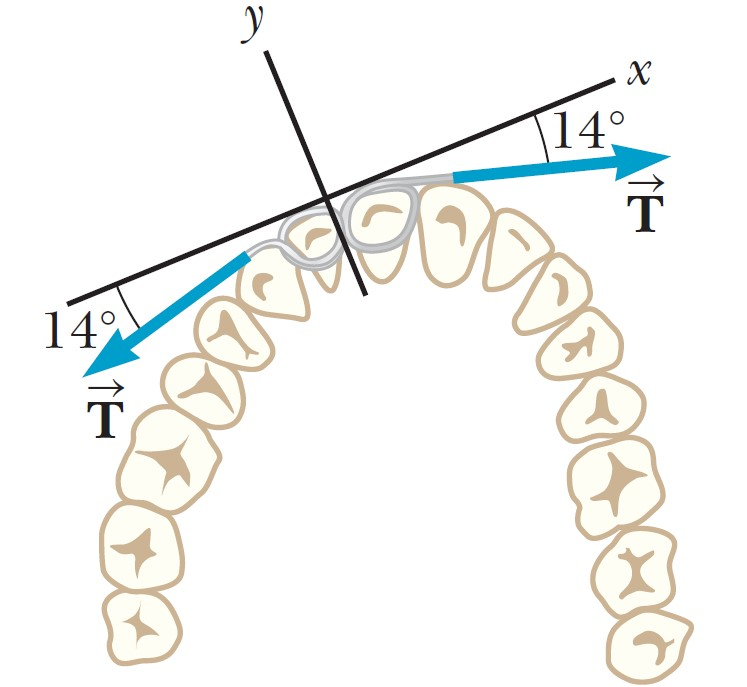
\includegraphics[width=0.5\linewidth]{../figs/D10-HKI-KTTX2-002-1}}
	\shortans[oly]{8,7}
	\loigiai{
		
	}
\end{ex}
% ===============================================================
\begin{ex}
	Một ô tô có khối lượng $m=\SI{1000}{\kilogram}$ chuyển động thẳng đều với tốc độ $v=\SI{18}{\kilo\meter/\hour}$ thì tài xế tắt máy xe. Lực ma sát tác dụng lên các bánh xe có độ lớn $\SI{500}{\newton}$ và không đổi. Xe đi thêm được bao xa nữa thì dừng lại?
	\shortans[oly]{25 }
	\loigiai{
		
	}
\end{ex}
% ===============================================================
\begin{ex}
	\immini{Một con nhện đang treo mình dưới một sợi tơ theo phương thẳng đứng thì bị một cơn gió thổi theo phương ngang làm dây treo lệch đi so với phương thẳng đứng một góc $\SI{30}{\degree}$. Biết trọng lượng của con nhện là $P=\SI{0.1}{\newton}$. Xác định độ lớn của lực mà gió tác dụng lên con nhện ở vị trí cân bằng trong hình bên \textit{(làm tròn kết quả đến chữ số hàng phần trăm)}.}
	{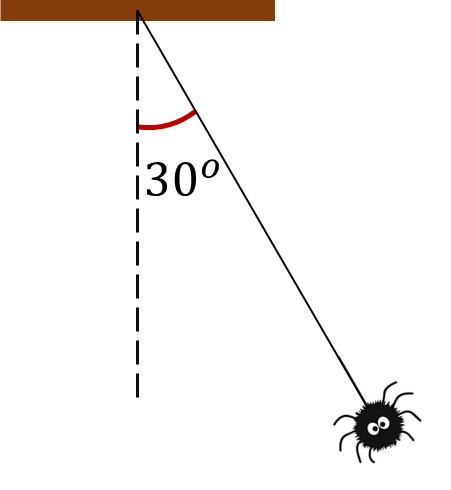
\includegraphics[width=0.45\linewidth]{../figs/D10-HKI-KTTX2-001-2}}
	\shortans[oly]{$0,06$}
	\loigiai{
		
	}
\end{ex}
\textit{Dữ kiện dùng chung cho câu 5 và câu 6:}\\
Một vật nhỏ có khối lượng $m=\SI{2}{\kilogram}$ đang nằm yên trên mặt phẳng ngang thì chịu tác dụng của lực kéo $\vec{F}_k$ theo phương nằm ngang. Vật bắt đầu trượt nhanh dần đều với gia tốc $\SI{2}{\meter/\second^2}$. Trong quá trình chuyển động, vật chịu tác dụng của lực cản có độ lớn $\SI{2}{\newton}$.
% ===============================================================
\begin{ex}
Tính độ lớn lực kéo tác dụng lên vật theo đơn vị newton $\left(\si{\newton}\right)$.	
	\shortans[oly]{6}
	\loigiai{
			}
\end{ex}
% ===============================================================
\begin{ex}
Sau khi vật chuyển động được 5 giây, lực kéo ngừng tác dụng. Tính tổng quãng đường vật đi được từ lúc bắt đầu chuyển động đến khi dừng lại theo đơn vị mét $\left(\si{\meter}\right)$.	
	\shortans[oly]{75}
	\loigiai{
		
	}
\end{ex}
\Closesolutionfile{ans}
\begin{center}
	\textbf{--- HẾT ---}
\end{center}\newpage
%\begin{center}
	\begin{tabular}{M{9.25cm}M{8.75cm}}
		\textbf{TRƯỜNG THCS-THPT NGUYỄN KHUYẾN}& \textbf{ÔN TẬP KTTX LẦN 2 HỌC KÌ I}\\
		\textbf{MÃ ĐỀ: 002}& \textbf{Bài thi môn: VẬT LÝ 10}\\
		\textit{(Đề thi có 05 trang)}& \textit{Thời gian làm bài: 40 phút, không kể phát đề}
		
		\noindent\rule{4cm}{0.8pt} \\
	\end{tabular}
\end{center}
\setcounter{section}{0}
\section{Câu trắc nghiệm nhiều phương án lựa chọn}
\textit{Thí sinh trả lời từ câu 1 đến câu 20. Mỗi câu hỏi thí sinh chọn một phương án}
\setcounter{ex}{0}
\Opensolutionfile{ans}[ans/D10-HKI-KTTX2-002-TN]
% ===================================================================
\begin{ex}
	Hệ thức nào sau đây là đúng theo định luật II Newton?
	\choice
	{\True $\vec{F}=m\vec{a}$}
	{$a=\dfrac{F}{m}$}
	{$\vec{a}=\dfrac{F}{m}$}
	{$\vec{F}=-m\vec{a}$}
	\loigiai{}
\end{ex}
% ===================================================================
\begin{ex}
	Khối lượng là đại lượng đặc trưng cho
	\choice
	{trọng lượng của vật}
	{tác dụng làm quay của lực quanh một trục}
	{thể tích của vật}
	{\True mức quán tính của vật}
	\loigiai{}
\end{ex}
% ===================================================================
\begin{ex}
Một chất điểm chịu tác dụng đồng thời của hai lực $\vec{F}_1$ và $\vec{F}_2$ thì hợp lực $\vec{F}$ của chúng luôn có độ lớn thỏa mãn hệ thức	
	\choice
	{$F=F_1-F_2$}
	{$F=F_1+F_2$}
	{\True $\left|F_1-F_2\right|\le F\le F_1+F_2$}
	{$F^2=F^2_1+F^2_2$}
	\loigiai{}
\end{ex}
% ===================================================================
\begin{ex}
	Một vật đang chuyển động nhanh dần đều dưới tác dụng của lực kéo mà lực đó đột ngột giảm độ lớn thì
	\choice
	{gia tốc của vật không đổi}
	{\True gia tốc của vật giảm}
	{gia tốc của vật tăng}
	{gia tốc và vận tốc của vật đều giảm}
	\loigiai{}
\end{ex}
% ===================================================================
\begin{ex}
	Khi đang đi xe đạp trên đường nằm ngang, nếu ta ngừng đạp, xe vẫn còn đi tiếp chưa dừng lại ngay là nhờ
	\choice
	{trọng lượng của xe}
	{lực ma sát}
	{\True quán tính của xe}
	{phản lực của mặt đường}
	\loigiai{}
\end{ex}
% ===================================================================
\begin{ex}
Theo định luật I Newton thì 	
	\choice
	{lực là nguyên nhân duy trì chuyển động}
	{\True một vật sẽ giữ nguyên trạng thái đứng yên hoặc chuyển động thẳng đều nếu nó không chịu tác dụng của lực nào}
	{một vật không thể chuyển động được nếu hợp lực tác dụng lên nó bằng 0}
	{mọi vật đang chuyển động đều có xu hướng dừng lại do quán tính}
	\loigiai{}
\end{ex}
% ===================================================================
\begin{ex}
	Một xe ô tô đang chuyển động thẳng với vận tốc không đổi là $\SI{20}{\meter/\second}$. Hợp lực tác dụng lên ô tô có độ lớn bằng
	\choice
	{$\SI{20}{\newton}$}
	{\True $0$}
	{$\SI{10}{\newton}$}
	{$\SI{-20}{\newton}$}
	\loigiai{}
\end{ex}
% ===================================================================
\begin{ex}
Khi một ô tô đột ngột phanh gấp thì người ngồi trong xe	
	\choice
	{ngả người về sau}
	{\True chúi người về phía trước}
	{ngả người sang bên cạnh}
	{dừng lại ngay}
	\loigiai{}
\end{ex}
% ===================================================================
\begin{ex}
	Những nhận định nào sau đây là đúng?
	\begin{enumerate}[label=\arabic*.]
		\item Khi vật chịu tác dụng của lực $\vec{F}$ thì gia tốc $\vec{a}$ mà vật thu được cùng phương nhưng ngược chiều với $\vec{F}$.
		\item Khi vật chỉ chịu tác dụng của lực $\vec{F}$ thì gia tốc $\vec{a}$ mà vật thu được cùng hướng với $\vec{F}$.
		\item Khi vật chịu tác dụng của hai lực cân bằng thì gia tốc $\vec{a}$ của vật thu được khác không.
		\item Khi vật chịu tác dụng của nhiều lực thì gia tốc $\vec{a}$ của vật thu được cùng hướng với lực tổng hợp tác dụng lên vật.
	\end{enumerate}
	\choice
	{\True 2, 4}
	{1, 3}
	{1, 4}
	{3, 4}
	\loigiai{}
\end{ex}
% ===================================================================
\begin{ex}
	Một lực $F_1$ không đổi, tác dụng lên vật khối lượng $m_1$ làm cho vật thu được gia tốc $a_1$.  Một lực $F_2$ không đổi, tác dụng lên vật khối lượng $m_2$ làm cho vật thu được gia tốc $a_2$. Nếu $F_2=F_1/3$ và $m_1=2m_2/5$ thì tỉ số $a_1/a_2$ bằng
	\choice
	{\True 15/2}
	{6/5}
	{11/15}
	{5/6}
	\loigiai{}
\end{ex}
% ===================================================================
\begin{ex}
	Tác dụng vào vật có khối lượng $\SI{3}{\kilogram}$ đang đứng yên một lực theo phương ngang thì vật này chuyển động nhanh dần đều với gia tốc $\SI{1.5}{\meter/\second^2}$. Độ lớn của lực này là
	\choice
	{$\SI{3}{\newton}$}
	{\True $\SI{4.5}{\newton}$}
	{$\SI{1.5}{\newton}$}
	{$\SI{2}{\newton}$}
	\loigiai{}
\end{ex}
% ===================================================================
\begin{ex}
	Một mẫu siêu xe có khối lượng $\SI{1.60}{\text{tấn}}$. Nếu coi xe tăng tốc đều và lực trung bình để tăng tốc xe là $\SI{24.0}{\kilo\newton}$ thì mẫu xe này cần bao lâu để có thể tăng tốc từ trạng thái nghỉ lên đến tốc độ $\SI{108}{\kilo\meter/\hour}$?
	\choice
	{\True Khoảng $\SI{2.00}{\second}$}
	{Khoảng $\SI{7.20}{\second}$}
	{Khoảng $\SI{10.0}{\second}$}
	{Khoảng $\SI{15.0}{\second}$}
	\loigiai{}
\end{ex}
% ===================================================================
\begin{ex}
	Một vật có khối lượng $m=\SI{10}{\kilogram}$ đang chuyển động thẳng đều với tốc độ $v=\SI{10}{\meter/\second}$ thì chịu tác dụng của một lực $\vec{F}$ không đổi, ngược hướng chuyển động và có độ lớn $F=\SI{10}{\newton}$.\\ Nhận định nào sau đây về chuyển động của vật là đúng?
	\choice
	{Vật dừng lại ngay}
	{\True Sau $\SI{10}{\second}$ kể từ lúc lực $\vec{F}$ tác dụng thì vật sẽ chuyển động theo chiều ngược lại}
	{Vật chuyển động chậm dần rồi dừng lại}
	{}
	\loigiai{}
\end{ex}
% ===================================================================
\begin{ex}
	Chất điểm khối lượng $\SI{2}{\kilogram}$ đứng yên dưới tác dụng của ba lực đồng qui có độ lớn lần lượt là $\SI{10}{\newton}$, $\SI{20}{\newton}$, $\SI{30}{\newton}$. Nếu bỏ đi lực $\SI{20}{\newton}$ thì
	\choice
	{chất điểm chuyển động thẳng đều}
	{chất điểm tiếp tục đứng yên}
	{\True chất điểm chuyển nhanh dần đều với gia tốc có độ lớn $\SI{10}{\meter/\second^2}$}
	{chất điểm chuyển nhanh dần đều với gia tốc có độ lớn $\SI{5}{\meter/\second^2}$}
	\loigiai{}
\end{ex}
% ===================================================================
\begin{ex}
	Một lực không đổi tác dụng vào một vật có khối lượng $\SI{7.5}{\kilogram}$ làm vật thay đổi tốc độ từ $\SI{8}{\meter/\second}$ đến $\SI{3}{\meter/\second}$ trong khoảng thời gian $\SI{2}{\second}$ nhưng vẫn giữ nguyên chiều chuyển động. Lực tác dụng vào vật có giá trị là
	\choice
	{$\SI{18.75}{\newton}$}
	{\True $\SI{-18.75}{\newton}$}
	{$\SI{20.5}{\newton}$}
	{$\SI{-20.5}{\newton}$}
	\loigiai{}
\end{ex}
% ===================================================================
\begin{ex}
	Một chất điểm chịu tác dụng của hai lực có độ lớn $\SI{18}{\newton}$ và $\SI{24}{\newton}$. Biết hợp lực của hai lực này có giá trị $\SI{30}{\newton}$, góc tạo bởi hai lực này là
	\choice
	{\True $\SI{90}{\degree}$}
	{$\SI{30}{\degree}$}
	{$\SI{45}{\degree}$}
	{$\SI{60}{\degree}$}
	\loigiai{}
\end{ex}
% ===================================================================
\begin{ex}
	Một xe tải chở hàng có tổng khối lượng xe và hàng hóa là 4 tấn, khởi hành với gia tốc $\SI{0.3}{\meter/\second^2}$. Khi không chở hàng, xe tải khởi hành với tốc $\SI{0.6}{\meter/\second^2}$. Biết rằng hợp lực tác dụng vào ô tô trong hai trường hợp đều bằng nhau. Khối lượng của xe lúc không chở hàng là
	\choice
	{1 tấn}
	{1,5 tấn}
	{\True 2 tấn}
	{2,5 tấn}
	\loigiai{}
\end{ex}
% ===================================================================
\begin{ex}
	Một xe tải không chở hàng đang chạy trên đường. Nếu người lái xe hãm phanh thì xe trượt một đoạn đường $\SI{12}{\meter}$ thì dừng lại. Nếu xe chở hàng có khối lượng hàng bằng hai lần khối lượng xe thì đoạn đường trượt bằng bao nhiêu? Cho rằng lực hãm và vận tốc ban đầu của xe tải không đổi.
	\choice
	{$\SI{4}{\meter}$}
	{$\SI{6}{\meter}$}
	{$\SI{24}{\meter}$}
	{\True $\SI{36}{\meter}$}
	\loigiai{}
\end{ex}
% ===================================================================
\begin{ex}
	Một vật nhỏ có khối lượng $\SI{10}{\kilogram}$ đang chuyển động với tốc độ $\SI{3}{\meter/\second}$ thì chịu tác động của một lực $\vec{F}$ cùng phương, cùng chiều chuyển động. Khi đó vật chuyển động nhanh dần đều và sau khi đi được thêm $\SI{32}{\meter}$ thì có tốc độ $\SI{5}{\meter/\second}$. Lực tác dụng vào vật có độ lớn bằng
	\choice
	{$\SI{0.25}{\newton}$}
	{\True $\SI{2.5}{\newton}$}
	{$\SI{25}{\newton}$}
	{$\SI{16}{\newton}$}
	\loigiai{}
\end{ex}
% ===================================================================
\begin{ex}
	Một lực tác dụng vào vật trong khoảng thời gian $\SI{0.6}{\second}$ làm vận tốc của nó thay đổi từ $\SI{8}{\centi\meter/\second}$ đến $\SI{5}{\centi\meter/\second}$ (lực cùng phương với phương chuyển động). Tiếp đó, tăng độ lớn của lực lên gấp đôi trong khoảng thời gian $\SI{2.2}{\second}$ nhưng vẫn giữ nguyên hướng của lực. Vận tốc của vật tại thời điểm cuối là
	\choice
	{$\SI{12}{\centi\meter/\second}$}
	{$\SI{15}{\centi\meter/\second}$}
	{\True $\SI{-17}{\centi\meter/\second}$}
	{$\SI{-20}{\centi\meter/\second}$}
	\loigiai{}
\end{ex}
\Closesolutionfile{ans}
\section{Câu trắc nghiệm đúng/sai} 
\textit{Thí sinh trả lời từ câu 1 đến câu 2. Trong mỗi ý \textbf{a)}, \textbf{b)}, \textbf{c)}, \textbf{d)} ở mỗi câu, thí sinh chọn đúng hoặc sai}
\setcounter{ex}{0}\\
\Opensolutionfile{ans}[ans/D10-HKI-KTTX2-002-TF]
% ===================================================================
\begin{ex}
	Một cậu bé đứng trên thùng xe của một chiếc xe bán tải đang chuyển động thẳng đều trên một đoạn đường nằm ngang. Cậu bé ném một lon nước ngọt theo phương thẳng đứng lên cao như hình minh họa bên dưới.
	\begin{center}
		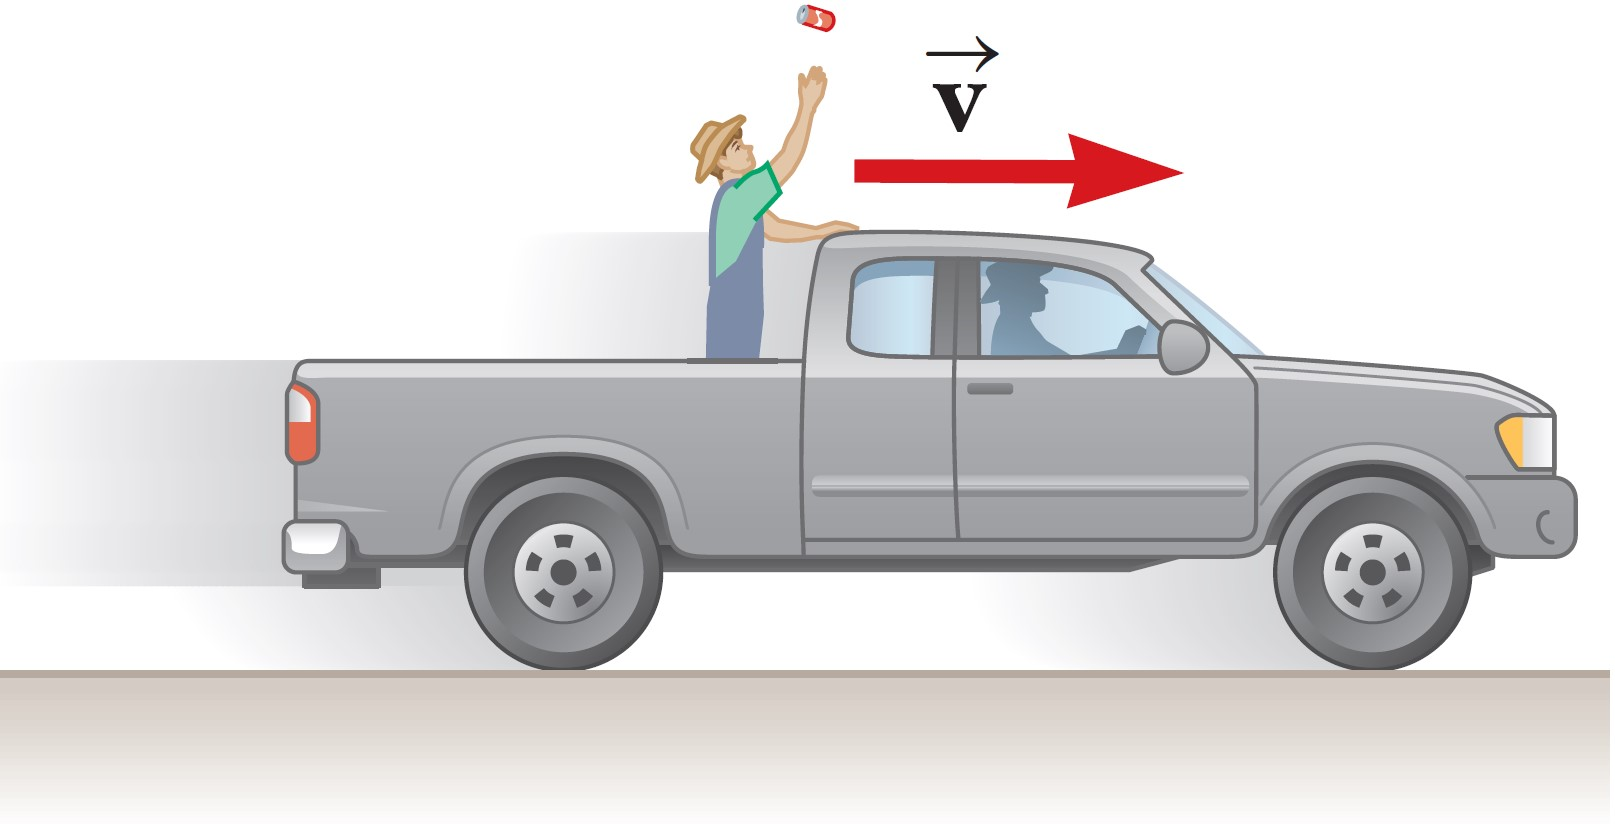
\includegraphics[width=0.4\linewidth]{figs/D10-HKI-KTTX2-001-4}
	\end{center}
	\choiceTF[t]
	{\True Lon nước ngọt sẽ rơi trở lại về tay cậu bé}
	{Đối với người quan sát đang đứng yên bên đường, lon nước ngọt chuyển động theo phương thẳng đứng}
	{\True Nếu xe tăng tốc trong quá trình lon nước rơi, lon nước sẽ rơi về phía sau cậu bé}
	{\True Nếu xe giảm tốc trong quá trình lon nước rơi, lon nước sẽ rơi về phía trước cậu bé}
	\loigiai{}
\end{ex}
% ===================================================================
\begin{ex}
	Hai thanh dầm thép đồng chất, có trọng tâm (điểm đặt của trọng lực) tại A và B, đặt chồng lên nhau như hình bên. Thanh dài hơn có trọng lượng $\SI{10}{\kilo\newton}$.
	\begin{center}
		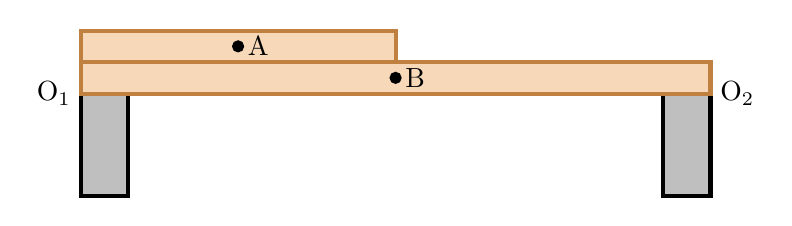
\begin{tikzpicture}
			\filldraw[line width=1.5pt, black, fill=gray!50!white] (0,-0.2) rectangle (0.6,-1.5);
			\filldraw[line width=1.5pt, black, fill=gray!50!white] (7.4,-0.2) rectangle (8,-1.5);
			\filldraw[line width=1.5pt, brown, fill=orange!60!brown!30!white] (0,-0.2) rectangle (8,0.2);
			\filldraw[line width=1.5pt, brown, fill=orange!60!brown!30!white] (0,0.2) rectangle (4,0.6);
			\filldraw (4,0) circle(2pt) node[right] {B};
			\filldraw (2,0.4) circle(2pt) node[right] {A};
			\node[left] at (0,-0.2) {O$_1$};
			\node[right] at (8,-0.2) {O$_2$};
		\end{tikzpicture}
	\end{center}
	Hai thanh dầm được đặt lên các cột đỡ tại $O_1$ và $O_2$. Hệ ở trạng thái cân bằng.
	\choiceTF[t]
	{\True Trọng lượng của thanh dầm ngắn hơn là $\SI{5}{\kilo\newton}$}
	{Hợp lực $\vec{P}$ của các trọng lực tác dụng lên hai thanh dầm có độ lớn $\SI{12.5}{\kilo\newton}$}
	{Khoảng cách từ giá của hợp lực $\vec{P}$ đến cột $O_1$ gấp 1,4 lần khoảng cách đến cột O$_2$}
	{\True Lực nâng của cột đỡ O$_1$ tác dụng lên thanh dầm có độ lớn $\SI{8.75}{\newton}$}
	\loigiai{}
\end{ex}
\Closesolutionfile{ans}
\section{Câu trắc nghiệm trả lời ngắn} \textit{Thí sinh trả lời từ câu 1 đến câu 6}
\setcounter{ex}{0}
\Opensolutionfile{ans}[ans/D10-HKI-KTTX2-002-TL]
% ===============================================================
\begin{ex}
	Một ô tô có các thông số gồm:
	\begin{center}
		\begin{tabular}{|M{5cm}|M{5cm}|M{5cm}|}
			\hline
		\thead{Khối lượng $\left(\si{\kilogram}\right)$} &\thead{Tải trọng $\left(\si{\kilogram}\right)$}&\thead{Tốc độ tối ưu $\left(\si{\kilo\meter/\hour}\right)$}\\
		\hline
		$\SI{2.10E3}{}$ & $950$ & $75,6$\\
		\hline
		\end{tabular}
	\end{center}
	Khi ô tô chở đủ tải trọng, nó có thể tăng tốc từ trạng thái nghỉ đến tốc độ tối ưu trong $\SI{3.00}{\text{giây}}$. Độ lớn lực tác dụng lên ô tô khi tăng tốc là bao nhiêu kilo newton $\left(\si{\kilo\newton}\right)$? \textit{(Làm tròn kết quả đến chữ số hàng phần mười)}.
	\shortans[oly]{21,4}
	\loigiai{
		
	}
\end{ex}
% ===============================================================
\begin{ex}
	Một quả bóng tennis khối lượng $\SI{56}{\gram}$ đang bay với tốc độ $\SI{20}{\meter/\second}$ thì đập trực diện vào bức tường và bật ngược trở lại với tốc độ $\SI{15}{\meter/\second}$. Thời gian quả bóng va chạm với tường là $\SI{0.05}{\second}$. Chọn chiều dương là chiều chuyển động ban đầu của quả bóng. Xác định lực do tường tác dụng lên quả bóng trong quá trình va chạm \textit{(làm tròn kết quả đến chữ số hàng đơn vị)}. 
	\shortans[oly]{$-39$}
	\loigiai{
		
	}
\end{ex}
% ===============================================================
\begin{ex}
	Một vật chịu tác dụng đồng thời của bốn lực như hình bên. Độ lớn của các lực lần lượt là $F_1=\SI{10}{\newton}$, $F_2=\SI{20}{\newton}$, $F_3=\SI{22}{\newton}$, $F_4=\SI{36}{\newton}$. Xác định độ lớn của hợp lực do các lực này tác dụng lên vật theo đơn vị newton $\left(\si{\newton}\right)$.
	\begin{center}
		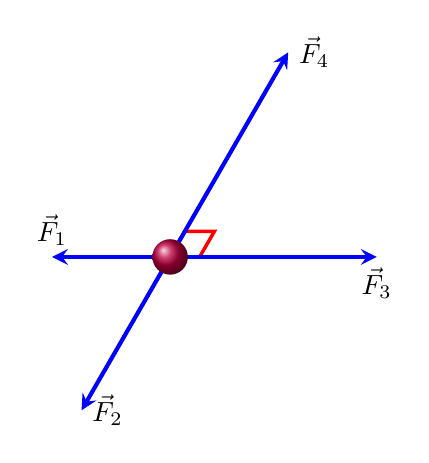
\begin{tikzpicture}[scale=0.75]
			\coordinate (O) at (0,0);
			\coordinate (N) at ($(O)+(60:4)$);
			\coordinate (B) at ($(O)+(-120:3)$);
			\coordinate (T) at ($(O)+(3.5,0)$);
			\coordinate (D) at ($(O)+(-2,0)$);
				\draw[-stealth, blue, line width=1.5pt] (O)--(D);
					\tkzMarkRightAngle[size=0.5,color=red, line width=1.25pt](T,O,N);
		\draw[-stealth, blue, line width=1.5pt] (O)--(T);
		\draw[-stealth, blue, line width=1.5pt] (O)--(N);
		\draw[-stealth, blue, line width=1.5pt] (O)--(B);
		\shade[ball color=purple] (0,0) circle (0.3cm);
		\node[below] at (T) {$\vec{F}_3$};
		\node[right] at (B) {$\vec{F}_2$};
		\node[right] at (N) {$\vec{F}_4$};
		\node[above] at (D) {$\vec{F}_1$};
		\end{tikzpicture}
	\end{center}
	\shortans[oly]{20}
	\loigiai{
		
	}
\end{ex}
% ===============================================================
\begin{ex}
Một cái đèn được treo vào hai sợi dây giống nhau như hình bên. Biết trọng lượng của đèn là $\SI{25}{\newton}$, hai dây làm thành góc $\SI{60}{\degree}$. Xác định lực căng của mỗi dây theo đơn vị newton $\left(\si{\newton}\right)$ \textit{(làm tròn kết quả đến chữ số hàng phần mười)}.
\begin{center}
	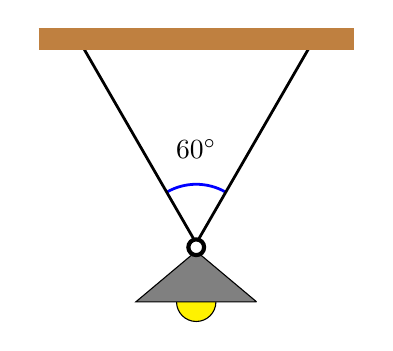
\begin{tikzpicture}
		\coordinate (O) at (0,0);
		\coordinate (A) at ($(O)+(60:3)$);
		\coordinate (B) at ($(O)+(120:3)$);
		\coordinate (C) at ($(0,-0.1)+(-40:1)$);
		\coordinate (D) at ($(0,-0.1)+(-140:1)$);
		\tkzMarkAngle[size=0.75cm,color=blue, line width=1pt](A,O,B);
		\tkzLabelAngle[color=black,pos=1.2](A,O,B){$\SI{60}{\degree}$}
		\draw[line width=1pt] (A)--(O)--(B);
		\draw[line width=8pt, brown] ($(B)+(-0.5,0)$)--($(A)+(0.5,0)$);
		\filldraw[fill=yellow] ($(C)!(O)!(D)$) circle (0.25);
		\filldraw[black, fill=gray] (C)--(0,-0.1)--(D)--(C);
		\filldraw[line width=1.5pt,fill=white] (0,-0.05) circle(0.1);
	\end{tikzpicture}
\end{center}	
	\shortans[oly]{14,4}
	\loigiai{
		
	}
\end{ex}

% ===============================================================
\begin{ex}
	Một vật có khối lượng $\SI{5}{\kilogram}$ được ném thẳng đứng hướng xuống với tốc độ ban đầu $\SI{2}{\meter/\second}$ từ độ cao $\SI{24}{\meter}$. Vật này rơi chạm đất sau $\SI{3}{\second}$ sau khi ném. Cho biết lực cản không khí tác dụng vào vật không đổi trong quá trình vật chuyển động và trọng lượng có độ lớn bằng 10 lần khối lượng. Tính độ lớn lực cản của không khí tác dụng vào vật theo đơn vị newton $\left(\si{\newton}\right)$.
	\shortans[oly]{30}
	\loigiai{
		
	}
\end{ex}
% ===============================================================
\begin{ex}
Đo những quãng đường đi được của một vật chuyển động thẳng biến đổi đều trong các khoảng thời gian liên tiếp bằng nhau và bằng $\SI{1.5}{\second}$, người ta thấy quãng đường sau dài hơn quãng đường trước $\SI{90}{\centi\meter}$. Biết khối lượng của vật là $\SI{250}{\gram}$. Tính độ lớn lực tác dụng lên vật theo đơn vị newton $\left(\si{\newton}\right)$. 	
	\shortans[oly]{0,1}
	\loigiai{
		
	}
\end{ex}
\Closesolutionfile{ans}
\begin{center}
	\textbf{--- HẾT ---}
\end{center}
%\newpage\begin{center}
	\begin{tabular}{M{9.25cm}M{8.75cm}}
		\textbf{TRƯỜNG THCS-THPT NGUYỄN KHUYẾN}& \textbf{ÔN TẬP KTTX LẦN 2 HỌC KÌ I}\\
		\textbf{MÃ ĐỀ: 001}& \textbf{Bài thi môn: VẬT LÝ 10}\\
		\textit{(Đề thi có 06 trang)}& \textit{Thời gian làm bài: 40 phút, không kể phát đề}
		
		\noindent\rule{4cm}{0.8pt} \\
	\end{tabular}
\end{center}
\setcounter{section}{0}
\begin{center}
	\textbf{\large BẢNG ĐÁP ÁN}
\end{center}
\section{}
\inputansbox{10}{ans/D10-HKI-KTTX2-001-TN}
\section{}
\inputansbox[2]{2}{ans/D10-HKI-KTTX2-001-TF}
\section{}
\inputansbox[3]{6}{ans/D10-HKI-KTTX2-001-TL}
%\newpage\begin{center}
	\begin{tabular}{M{9.25cm}M{8.75cm}}
		\textbf{TRƯỜNG THCS-THPT NGUYỄN KHUYẾN}& \textbf{ÔN TẬP KTTX LẦN 2 HỌC KÌ I}\\
		\textbf{MÃ ĐỀ: 002}& \textbf{Bài thi môn: VẬT LÝ 10}\\
		\textit{(Đề thi có 06 trang)}& \textit{Thời gian làm bài: 40 phút, không kể phát đề}
		
		\noindent\rule{4cm}{0.8pt} \\
	\end{tabular}
\end{center}
\setcounter{section}{0}
\begin{center}
	\textbf{\large BẢNG ĐÁP ÁN}
\end{center}
\section{}
\inputansbox{10}{ans/D10-HKI-KTTX2-002-TN}
\section{}
\inputansbox[2]{2}{ans/D10-HKI-KTTX2-002-TF}
\section{}
\inputansbox[3]{6}{ans/D10-HKI-KTTX2-002-TL}
% ======================= ÔN TẬP KIỂM TRA CUỐI KÌ I
%\begin{center}
	\begin{tabular}{M{9.25cm}M{8.75cm}}
		\textbf{TRƯỜNG THCS-THPT NGUYỄN KHUYẾN}& \textbf{ÔN TẬP KIỂM TRA CUỐI HỌC KÌ I}\\
		\textbf{MÃ ĐỀ: 001}& \textbf{Bài thi môn: VẬT LÝ 10}\\
		\textit{(Đề thi có 04 trang)}& \textit{Thời gian làm bài: 45 phút, không kể phát đề}
		
		\noindent\rule{4cm}{0.8pt} \\
	\end{tabular}
\end{center}
\setcounter{section}{0}
\section{Câu trắc nghiệm nhiều phương án lựa chọn}
\textit{Thí sinh trả lời từ câu 1 đến câu 18. Mỗi câu hỏi thí sinh chọn một phương án}
\setcounter{ex}{0}
\Opensolutionfile{ans}[ans/D10-CK1-001-TN]

% ===================================================================
\begin{ex}
	Đại lượng đặc trưng cho mức quán tính của một vật là
	\choice
	{vận tốc của vật}
	{\True khối lượng của vật}
	{kích thước của vật}
	{gia tốc của vật}
	\loigiai{}
\end{ex}
% ===================================================================
\begin{ex}
	Gia tốc rơi tự do phụ thuộc vào yếu tố nào?
	\choice
	{Quãng đường vật đi được}
	{\True Vĩ độ địa lí và độ cao}
	{Vĩ độ địa lí}
	{Độ cao}
	\loigiai{}
\end{ex}
% ===================================================================
\begin{ex}
	Lực căng dây \textbf{không có} đặc điểm nào sau đây?
	\choice
	{\True Độ lớn luôn bằng trọng lượng của vật}
	{Phương trùng với phương sợi dây}
	{Điểm đặt ở hai đầu dây, chỗ tiếp xúc với vật}
	{Chiều luôn hướng vào giữa sợi dây}
	\loigiai{}
\end{ex}
% ===================================================================
\begin{ex}
	Trong chuyển động thẳng biến đổi đều, đại lượng không đổi theo thời gian là
	\choice
	{tọa độ}
	{quãng đường}
	{vận tốc}
	{\True gia tốc}
	\loigiai{}
\end{ex}

% ===================================================================
\begin{ex}
	Câu nào sau đây là đúng khi nói về lực hấp dẫn do Trái Đất tác dụng lên Mặt Trăng và do Mặt Trăng tác dụng lên Trái Đất?
	\choice
	{Hai lực này cùng phương cùng chiều}
	{\True Hai lực này cùng phương ngược chiều}
	{Hai lực này cùng chiều, cùng độ lớn}
	{Phương của hai lực này không thay đổi và luôn trùng nhau}
	\loigiai{}
\end{ex}
% ===================================================================
\begin{ex}
	Một vật chuyển động thẳng đều khi
	\choice
	{hợp lực tác dụng vào nó cùng chiều chuyển động}
	{\True các lực tác dụng vào nó cân bằng nhau}
	{hợp lực tác dụng vào nó không đổi}
	{hợp lực tác dụng vào nó ngược chiều chuyển động}
	\loigiai{}
\end{ex}
% ===================================================================
\begin{ex}
	Hệ số ma sát giữa hai mặt tiếp xúc sẽ thay đổi như thế nào nếu lực ép hai mặt đó tăng lên?
	\choice
	{Tăng lên}
	{Giảm đi}
	{\True Không thay đổi}
	{Còn phụ thuộc vào diện tích hai bề mặt}
	\loigiai{}
\end{ex}
% ===================================================================
\begin{ex}
	\immini{Trên hình bên là đồ thị tọa độ - thời gian của một vật chuyển động thẳng. Hãy cho biết thông tin nào sau đây là \textbf{sai}?
		\choice
		{Tọa độ ban đầu của vật là $x_0=\SI{10}{\meter}$}
		{\True Trong $\SI{5}{\second}$ đầu tiên, vật đi được $\SI{25}{\meter}$}
		{Vật chuyển động theo chiều dương của trục tọa độ}
		{Gốc thời gian được chọn là thời điểm vật ở cách gốc tọa độ $\SI{10}{\meter}$}}
		{
		\begin{tikzpicture}  
			\begin{axis}[  ultra thick,
				xmin=0,  
				xmax=7,  
				xtick={0,5},
				ytick={0,10,25},
				ymin=0,  
				ymax=30, 
				samples=300,
				axis lines=center, 
				xlabel=$\xsi{t}{\left(\si{\second}\right)}$, 		ylabel=$\xsi{x}{\left(\si{\meter}\right)}$,
				every axis y label/.style={at=(current axis.above origin),anchor=south},  
				every axis x label/.style={at=(current axis.right of origin),anchor=west},  scale=0.5]
				\draw[line width=1pt, dashed] (axis cs: 0,25)--(axis cs: 5,25)--(axis cs: 5,0);
				\addplot [line width=1.5pt, blue, smooth, domain=0:5] {10+3*x};  
				\coordinate (O) at (axis cs: 0,0);
			\end{axis}  
			\node[below left] at (O) {0};
		\end{tikzpicture}
		}
	\loigiai{}
\end{ex}
% ===================================================================
\begin{ex}
Một đoàn tàu rời ga chuyển động thẳng nhanh dần, sau 1 phút đạt vận tốc $\SI{40}{\kilo\meter/\hour}$. Gia tốc trung bình của đoàn tàu gần giá trị nào sau đây nhất?	
	\choice
	{$\SI{0.188}{\meter/\second^2}$}
	{$\SI{0.288}{\meter/\second^2}$}
	{$\SI{0.285}{\meter/\second^2}$}
	{\True $\SI{0.185}{\meter/\second^2}$}
	\loigiai{}
\end{ex}
% ===================================================================
\begin{ex}
	Hình vẽ nào sau đây biểu diễn đúng lực tổng hợp $\vec{F}$ của hai lực $\vec{F}_1$ và $\vec{F}_2$?
	\choice
	{\begin{tikzpicture}
			\coordinate (A) at (0,0);
			\coordinate (B) at ($(A)+(2.5,0)$);
			\coordinate (C) at ($(B)+(90:1.5)$);
			\draw[blue, line width=1.5pt, -stealth] (A)--(B);
			\draw[blue, line width=1.5pt, -stealth] (B)--(C);
			\draw[blue, line width=1.5pt, -stealth] (A)--(C);
			\node[below, blue] at ($(A)!0.5!(B)$) {$\vec{F}$};
			\node[right, blue] at ($(B)!0.5!(C)$) {$\vec{F}_2$};
			\node[above left, blue] at ($(A)!0.5!(C)$) {$\vec{F}_1$};
	\end{tikzpicture}}
	{\begin{tikzpicture}
			\coordinate (O) at (0,0);
			\coordinate (A) at (2,0);
			\coordinate (C) at ($(A)+(-60:1.5)$);
			\coordinate (B) at ($(O)+(-60:1.5)$);
			\draw[dashed, line width=1pt] (A)--(C)--(B);
			\draw[-stealth, blue, line width=1.5pt] (O)--(A);
			\draw[-stealth, blue, line width=1.5pt] (O)--(B);
			\draw[-stealth, blue, line width=1.5pt] (O)--(C);
			\node[below left, blue] at ($(O)!0.5!(B)$) {$\vec{F}$};
			\node[above, blue] at ($(O)!0.5!(A)$) {$\vec{F}_1$};
			\node[below, blue] at ($(O)!0.5!(C)$) {$\vec{F}_2$};
	\end{tikzpicture}}
	{\True \begin{tikzpicture}
			\coordinate (O) at (0,0);
			\coordinate (A) at ($(O)+(90:2.5)$);
			\coordinate (B) at ($(O)+(180:2)$);
			\coordinate (C) at ($(A)+(180:2)$);
			\draw[dashed, line width=1pt] (A)--(C)--(B);
			\draw[blue, line width=1.5pt, -stealth] (O)--(A);
			\draw[blue, line width=1.5pt, -stealth] (O)--(C);
			\draw[blue, line width=1.5pt, -stealth] (O)--(B);
			\node[above right, blue] at ($(O)!0.5!(C)$) {$\vec{F}$};
			\node[above, blue] at ($(O)!0.5!(B)$) {$\vec{F}_2$};
			\node[right, blue] at ($(O)!0.5!(A)$) {$\vec{F}_1$};
	\end{tikzpicture}}
	{\begin{tikzpicture}
			\coordinate (O) at (0,0);
			\coordinate (A) at ($(O)+(2,0)$);
			\coordinate (B) at ($(O)+(60:2)$);
			\draw[blue, -stealth, line width=1.5pt] (O)--(A);
			\draw[blue, -stealth, line width=1.5pt] (O)--(B);
			\draw[blue, -stealth, line width=1.5pt] (A)--(B);
			\node[above, blue] at ($(O)!0.5!(A)$) {$\vec{F}_2$};
			\node[right, blue] at ($(A)!0.5!(B)$) {$\vec{F}$};
			\node[left, blue] at ($(O)!0.5!(B)$) {$\vec{F}_1$};
	\end{tikzpicture}}
	\loigiai{}
\end{ex}
% ===================================================================
\begin{ex}
\immini{Một vật chuyển động thẳng có đồ thị vận tốc - thời gian như hình bên. Tính chất chuyển động của vật là	
	\choice
	{Chuyển động chậm dần đều theo chiều dương rồi nhanh dần đều theo chiều âm}
	{Chuyển động nhanh dần đều theo chiều dương rồi chậm dần đều theo chiều âm}
	{\True Chuyển động nhanh dần đều rồi chậm dần đều theo chiều dương}
	{Chuyển động nhanh dần đều rồi chậm dần đều theo chiều âm}}
	{
	\begin{tikzpicture}  
		\begin{axis}[  ultra thick,
			xmin=0,  
			xmax=45,  
			xtick={0,15,40},
			ytick={0,30},
			ymin=0,  
			ymax=40, 
			samples=300,
			axis lines=center, 
			xlabel=$\xsi{t}{\left(\si{\second}\right)}$, 		ylabel=$\xsi{v}{\left(\si{\meter/\second}\right)}$,
			every axis y label/.style={at=(current axis.above origin),anchor=south},  
			every axis x label/.style={at=(current axis.right of origin),anchor=west},  scale=0.5]
			\draw[line width=1pt, dashed] (axis cs: 0,30)--(axis cs: 15,30)--(axis cs: 15,0);
			\addplot [line width=1.5pt, blue, smooth, domain=0:15] {2*x};  
			\addplot [line width=1.5pt, blue, smooth, domain=15:40] {30-1.2*(x-15)}; 
			\coordinate (O) at (axis cs: 0,0);
		\end{axis}  
		\node[below left] at (O) {0};
	\end{tikzpicture}
	}
	\loigiai{}
\end{ex}
% ===================================================================
\begin{ex}
	Một lực không đổi tác dụng vào một vật có khối lượng $\SI{5.0}{\kilogram}$ làm vận tốc của nó tăng dần từ $\SI{2.0}{\meter}$ đến $\SI{8.0}{\meter/\second}$ trong $\SI{3.0}{\second}$. Độ lớn lực tác dụng vào vật là
	\choice
	{\True $\SI{10}{\newton}$}
	{$\SI{5}{\newton}$}
	{$\SI{15}{\newton}$}
	{$\SI{1}{\newton}$}
	\loigiai{}
\end{ex}
% ===================================================================
\begin{ex}
Cho biết khối lượng của Trái Đất là $M=\SI{6E24}{\kilogram}$; khối lượng của một hòn đá $m=\SI{2.3}{\kilogram}$; gia tốc trọng trường là $g=\SI{9.81}{\meter/\second^2}$. Hòn đá hút Trái Đất một lực có độ lớn xấp xỉ
	\choice
	{$\SI{15.82}{\newton}$}
	{$\SI{20.24}{\newton}$}
	{\True $\SI{22.56}{\newton}$}
	{$\SI{32}{\newton}$}
	\loigiai{}
\end{ex}
% ===================================================================
\begin{ex}
	Một dòng sông rộng $\SI{100}{\meter}$ và dòng nước chảy với vận tốc $\SI{3}{\meter/\second}$ so với bờ. Một chiếc thuyền đi ngang sông với vận tốc $\SI{4}{\meter/\second}$ so với dòng nước. Quãng đường mà thuyền đi được khi sang đến bờ bên kia là
	\choice
	{$\SI{150}{\meter}$}
	{\True $\SI{125}{\meter}$}
	{$\SI{100}{\meter}$}
	{$\SI{50}{\meter}$}
	\loigiai{}
\end{ex}
% ===================================================================
\begin{ex}
	Một vật có khối lượng $\SI{70}{\kilogram}$ chuyển động thẳng đều trên mặt sàn nằm ngang dưới tác dụng của lực kéo không đổi và có độ lớn $\SI{210}{\newton}$ theo phương ngang. Lấy $g=\SI{10}{\meter/\second^2}$. Hệ số ma sát trượt giữa vật và sàn là
	\choice
	{\True $0,3$}
	{$0,147$}
	{$3,3$}
	{$0,05$}
	\loigiai{}
\end{ex}
% ===================================================================
\begin{ex}
	Một vật khối lượng $\SI{2.5}{\kilogram}$ rơi thẳng đứng từ độ cao $\SI{100}{\meter}$ không vận tốc đầu, sau $\SI{20}{\second}$ thì chạm đất. Lấy gia tốc trọng trường $g=\SI{10}{\meter/\second^2}$. Nếu coi lực cản không khí tác dụng lên vật trong quá trình rơi là không đổi thì độ lớn của lực cản là
	\choice
	{$\SI{20}{\newton}$}
	{$\SI{40}{\newton}$}
	{\True $\SI{23.75}{\newton}$}
	{$\SI{25}{\newton}$}
	\loigiai{}
\end{ex}
% ===================================================================
\begin{ex}
Một vật chuyển động nhanh dần đều không vận tốc đầu. Trong giây thứ nhất vật đi được đoạn đường $s_1=\SI{3}{\meter}$, trong giây thứ hai vật đi được quãng đường $s_2$ bằng	
	\choice
	{$\SI{6}{\meter}$}
	{$\SI{3}{\meter}$}
	{\True $\SI{9}{\meter}$}
	{$\SI{12}{\meter}$}
	\loigiai{}
\end{ex}
% ===================================================================
\begin{ex}
	Một quả bóng có khối lượng $\SI{300}{\gram}$ bay với vận tốc $\SI{72}{\kilo\meter/\hour}$ đến đập vuông góc vào một bức tường thẳng đứng rồi bật trở lại theo phương cũ với vận tốc $\SI{54}{\kilo\meter/\hour}$. Thời gian va chạm $\SI{0.14}{\second}$. Lực do tường tác dụng lên quả bóng có độ lớn là
	\choice
	{\True $\SI{75}{\newton}$}
	{$\SI{70}{\newton}$}
	{$\SI{85}{\newton}$}
	{$\SI{65}{\newton}$}
	\loigiai{}
\end{ex}
\Closesolutionfile{ans}
\section{Câu trắc nghiệm đúng/sai} 
\textit{Thí sinh trả lời từ câu 1 đến câu 4. Trong mỗi ý \textbf{a)}, \textbf{b)}, \textbf{c)}, \textbf{d)} ở mỗi câu, thí sinh chọn đúng hoặc sai}
\setcounter{ex}{0}\\
\Opensolutionfile{ans}[ans/D10-CK1-001-TF]
% ===================================================================
\begin{ex}
	Nhận định các phát biểu sau về vai trò của lực ma sát nghỉ.\\
	Lực ma sát nghỉ
	\choiceTF[t]
	{\True đóng vai trò là lực phát động trong trường hợp chuyển động của người đi bộ, xe đạp, ô tô, tàu hỏa, \dots}
	{\True giúp ta cầm, nắm các vật}
	{giúp xe chuyển động chậm lại khi hãm phanh}
	{\True đóng vai trò truyền chuyển động bằng dây curoa trong các máy móc, băng chuyền, \dots}
	\loigiai{}
\end{ex}
% ===================================================================
\begin{ex}
	\immini{Một quả khúc côn cầu có khối lượng $\SI{0.30}{\kilogram}$ đang nằm trên mặt băng cứng, hoàn toàn nhẵn nằm ngang, thì chịu tác dụng đồng thời của hai cú đánh như hình bên. Lực $\vec{F}_1$ do cú đánh thứ nhất có độ lớn $\SI{5.0}{\newton}$ làm với trục $x$ về phía dưới một góc $\SI{20}{\degree}$. Lực $\vec{F}_2$ do cú đánh thứ hai có độ lớn $\SI{8.0}{\newton}$ làm với trục $x$ về phía trên một góc $\SI{60}{\degree}$.} {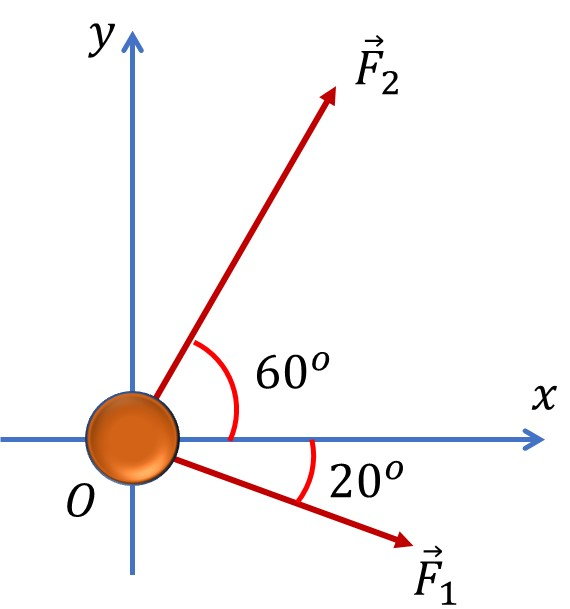
\includegraphics[scale=0.35]{figs/D10-CK1-002-2}}
	\choiceTF[t]
	{\True Hợp lực tác dụng lên quả khúc côn cầu có độ lớn $\SI{10.14}{\newton}$}
	{\True Sau cú đánh, quả khúc côn cầu chuyển động theo hướng hợp với trục $x$ góc $\SI{31}{\degree}$}
	{\True Trọng lực tác dụng lên quả khúc côn cầu không gây ra gia tốc cho nó}
	{\True Gia tốc của quả khúc côn cầu ngay sau cú đánh kép xấp xỉ $\SI{34}{\meter/\second^2}$}
	\loigiai{}
\end{ex}

% ===================================================================
\begin{ex}
\immini{	Huyền thoại điền kinh Usain Bolt người Jamaica đã lập kỉ lục thế giới ở nội dung chạy $\SI{100}{\meter}$ vào tháng 8/2009 tại Berlin. Usain Bolt đã hoàn thành cự li trên với thời gian $\SI{9.58}{\second}$. Ta giả sử rằng Bolt tăng tốc đều trong $\SI{3.00}{\second}$ đầu tiên để đạt tốc độ tối đa và duy trì tốc độ đó trong suốt phần còn lại của cuộc đua.}
{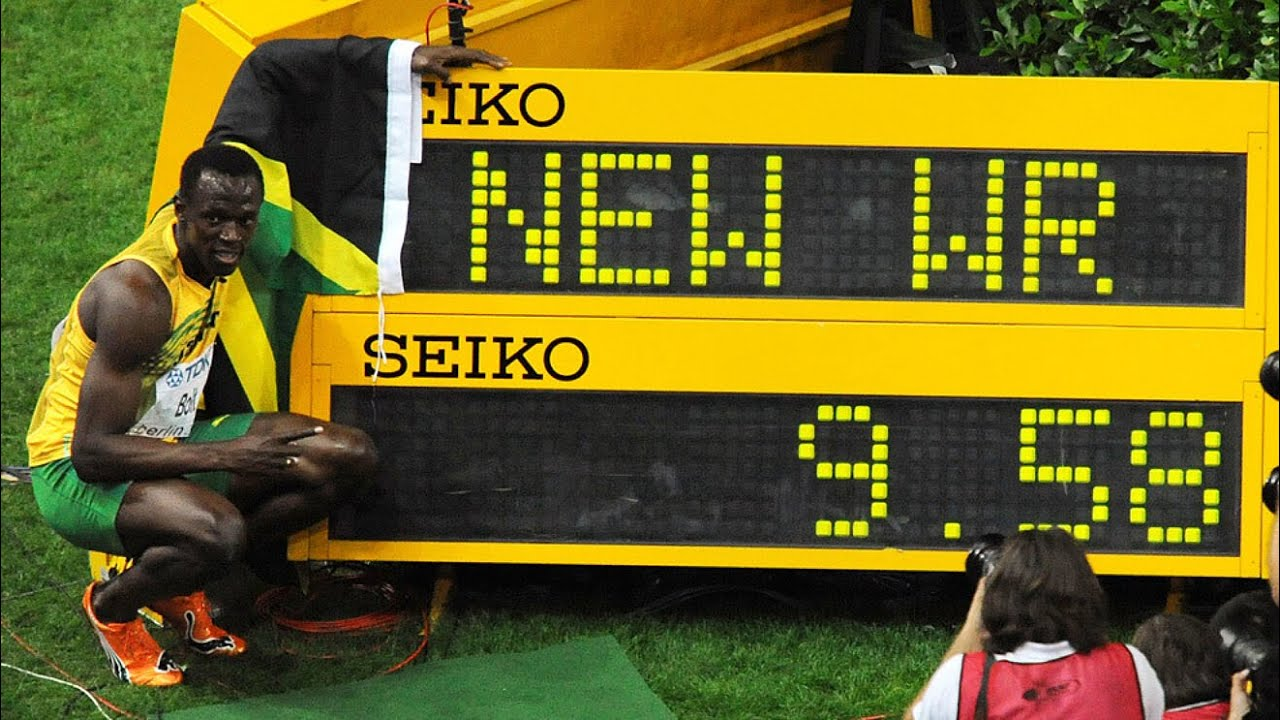
\includegraphics[scale=0.08]{figs/D10-CK1-001-5}}
	\choiceTF[t]
	{Chuyển động của Usain Bolt là chuyển động thẳng nhanh dần đều}
	{\True Tốc độ của Usain Bolt khi về đến đích xấp xỉ $\SI{12.38}{\meter/\second}$}
	{Gia tốc trong giai đoạn tăng tốc của Usain Bolt là khoảng $\SI{6}{\meter/\second^2}$}
	{\True Usain Bolt đã duy trì tốc độ tối đa của mình trên đoạn đường dài $\SI{81.46}{\meter}$}
	\loigiai{}
\end{ex}
% ===================================================================
\begin{ex}
\immini{Một vật nhỏ có khối lượng $\SI{5.0}{\kilogram}$ được kéo bằng sợi dây trên sàn nằm ngang. Sợi dây nhẹ, không dãn và làm góc $\SI{25}{\degree}$ so với phương ngang. Hệ số ma sát trượt giữa vật và mặt sàn là $0,15$. Lực kéo tác dụng lên dây có độ lớn $F=\SI{12}{\newton}$. Lấy $g=\SI{9.8}{\meter/\second^2}$.}
{\begin{tikzpicture}
		\coordinate (O) at (0,0);
		\coordinate (A) at ($(O)+(2.5,0)$);
		\coordinate (B) at ($(O)+(25:2)$);
		\filldraw[color=orange!80!brown] (-0.5,-0.25) rectangle (0.5,0.25);
		\draw[line width=6pt, color=gray] (-2.5,-0.36)--(2.5,-0.36);
		\draw[-stealth, blue, line width=1.5pt] (O)--(B);
		\draw[dashed, line width=1pt] (O)--(A);
		\tkzMarkAngle[size=0.75cm,color=red, line width=1.2pt](A,O,B);
		\tkzLabelAngle[color=black,pos=1.2](A,O,B){$\SI{25}{\degree}$};
		\node[above, blue]at(B) {$\vec{F}$};
\end{tikzpicture}}
	\choiceTF[t]
	{Phản lực của mặt sàn tác dụng lên vật bằng $\SI{49}{\newton}$}
	{\True Lực ma sát trượt tác dụng lên vật có độ lớn xấp xỉ $\SI{6.6}{\newton}$}
	{Gia tốc của vật xấp xỉ $\SI{1.08}{\meter/\second^2}$}
	{Người ta tăng dần lực kéo $F$, ngay khi lực kéo có độ lớn $\SI{49}{\newton}$ thì vật bị nâng khỏi mặt sàn}
	\loigiai{}
\end{ex}
\Closesolutionfile{ans}
\section{Câu trắc nghiệm trả lời ngắn} \textit{Thí sinh trả lời từ câu 1 đến câu 6}
\setcounter{ex}{0}
\Opensolutionfile{ans}[ans/D10-CK1-001-TL]
% ===============================================================
\begin{ex}
	Một chất điểm chuyển động thẳng có phương trình vận tốc theo thời gian dạng $v=15-3t$, trong đó $t$ tính bằng giây và $v$ tính bằng $\si{\meter/\second}$. Tính tốc độ trung bình của chất điểm trong khoảng thời gian từ $t_1=\SI{0}{\second}$ đến $t_2=\SI{2}{\second}$ theo đơn vị mét/giây $\left(\si{\meter/\second}\right)$.
	\shortans[oly]{12}
	\loigiai{
		
	}
\end{ex}
% ===============================================================
\begin{ex}
	Một vật khối lượng $m=\SI{1.5}{\kilogram}$ bắt đầu chuyển động nhanh dần đều trên mặt phẳng ngang dưới tác dụng của lực kéo theo phương ngang, độ lớn $F_{\mathrm{k}}=\SI{7.5}{\newton}$. Hệ số ma sát giữa vật và mặt phẳng ngang là $\mu=0,2$. Lấy $g=\SI{10}{\meter/\second^2}$. Tính gia tốc của vật theo đơn vị $\si{\meter/\second^2}$.
	\shortans[oly]{3}
	\loigiai{
		
	}
\end{ex}
% ===============================================================
\begin{ex}
\immini{Một vòng đệm bằng đồng có đường kính ngoài và đường kính trong lần lượt là $\SI{4.50}{\centi\meter}$ và $\SI{1.25}{\centi\meter}$. Bề dày của vòng đệm là $\SI{1.50}{\milli\meter}$. Đồng có khối lượng riêng là $\SI{8600}{\kilogram/\meter^3}$. Lấy gia tốc trọng trường $g=\SI{9.8}{\meter/\second^2}$, $\pi=3,14$. Trọng lượng của vòng đệm trên là bao nhiêu newton $\left(\si{\newton}\right)$? \textit{(Kết quả làm tròn đến chữ số hàng phần mười)}.}
{
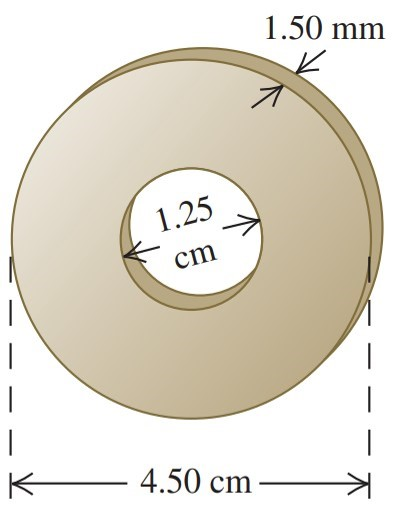
\includegraphics[scale=0.4]{figs/D10-CK1-001-3}
}
	\shortans[oly]{0,2}
	\loigiai{
		
	}
\end{ex}

% ===============================================================
\begin{ex}
	\immini{Một khối hộp có dạng hình lập phương nặng $\SI{1}{\kilogram}$  đặt trong nước nguyên chất có khối lượng riêng $\rho=\SI{1000}{\kilogram/\meter^3}$. Mỗi cạnh của khối hộp có độ dài $\SI{10}{\centi\meter}$. Cho $g=\SI{10}{\meter/\second^2}$. Tính lực đẩy Archimedes tác dụng lên khối hộp nếu nó được nhúng hoàn toàn trong nước. \textit{(Kết quả tính theo đơn vị newton $\left(\si{\newton}\right)$)}.}
	{\includegraphics[scale=0.4]{figs/D10-CK1-001-1}}
	\shortans[oly]{10}
	\loigiai{
		
	}
\end{ex}
% ===============================================================
\begin{ex}
	\immini{Một cơ hệ bố trí như hình bên được sử dụng trong bệnh viện để hỗ trợ tác dụng lực kéo ngang lên chân bị thương của bệnh nhân. Lấy gia tốc trọng trường $g=\SI{9.8}{\meter/\second^2}$. Tính độ lớn hợp lực kéo ngang tác dụng lên giá đỡ bàn chân theo đơn vị newton $\left(\si{\newton}\right)$. \textit{(Kết quả làm tròn đến chữ số hàng đơn vị)}.}{
		\includegraphics[scale=0.35]{figs/D10-CK1-001-6}
	}
	\shortans[oly]{105}
	\loigiai{
		
	}
\end{ex}
% ===============================================================
\begin{ex}
\immini{Một vật khối lượng $m=\SI{1}{\kilogram}$ có thể trượt trên mặt phẳng nghiêng góc $\alpha=\SI{30}{\degree}$ so với mặt ngang. Hệ số ma sát giữa vật và mặt phẳng nghiêng là $\mu=0,2$. Lực $\vec{F}$  không đổi tác dụng vào vật có phương nằm ngang (hình vẽ). Lấy $g=\SI{10}{\meter/\second^2}$.	Xác định độ lớn của lực $\vec{F}$ để vật trượt đều lên mặt phẳng nghiêng. \textit{(Kết quả tính theo đơn vị $\si{\newton}$ và làm tròn đến chữ số hàng phần mười)}.
}
{\includegraphics[scale=0.8]{figs/D10-CK1-001-2}}
	\shortans[oly]{ 8,8}
	\loigiai{
		
	}
\end{ex}
\Closesolutionfile{ans}
\begin{center}
	\textbf{--- HẾT ---}
\end{center}\newpage
%\begin{center}
	\begin{tabular}{M{9.25cm}M{8.75cm}}
		\textbf{TRƯỜNG THCS-THPT NGUYỄN KHUYẾN}& \textbf{ÔN TẬP KIỂM TRA CUỐI HỌC KÌ I}\\
		\textbf{MÃ ĐỀ: 002}& \textbf{Bài thi môn: VẬT LÝ 10}\\
		\textit{(Đề thi có 04 trang)}& \textit{Thời gian làm bài: 45 phút, không kể phát đề}
		
		\noindent\rule{4cm}{0.8pt} \\
	\end{tabular}
\end{center}
\setcounter{section}{0}
\section{Câu trắc nghiệm nhiều phương án lựa chọn}
\textit{Thí sinh trả lời từ câu 1 đến câu 18. Mỗi câu hỏi thí sinh chọn một phương án}
\setcounter{ex}{0}
\Opensolutionfile{ans}[ans/D10-CK1-002-TN]
% ===================================================================
\begin{ex}
	Người ta thường dùng quãng đường đi được trong cùng một đơn vị thời gian để xác định độ nhanh, chậm của chuyển động. Đại lượng này gọi là
	\choice
	{vận tốc trung bình}
	{\True tốc độ trung bình}
	{tốc độ tức thời}
	{vận tốc tức thời}
	\loigiai{}
\end{ex}
% ===================================================================
\begin{ex}
	Điều nào sau đây là \textbf{sai} khi nói về trọng lực?
	\choice
	{Trọng lực được xác định bởi biểu thức $\vec{P}=m\cdot\vec{g}$}
	{Điểm đặt của trọng lực là trọng tâm của vật}
	{\True Trọng lực có độ lớn tỉ lệ nghịch với khối lượng của vật}
	{Trọng lực là lực hút của Trái Đất tác dụng lên vật}
	\loigiai{}
\end{ex}
% ===================================================================
\begin{ex}
Trong một cơn giông, một cành cây bị gãy và bay trúng vào một cửa kính, làm vỡ kính. Chọn nhận xét đúng.	
	\choice
	{Lực của cành cây tác dụng lên tấm kính lớn hơn lực của tấm kính tác dụng vào cành cây}
	{\True Lực của cành cây tác dụng lên tấm kính có độ lớn bằng lực của tấm kính tác dụng vào cành cây}
	{Lực của cành cây tác dụng lên tấm kính nhỏ hơn lực của tấm kính tác dụng vào cành cây}
	{Cành cây không tương tác với tấm kính khi làm vỡ kính}
	\loigiai{}
\end{ex}
% ===================================================================
\begin{ex}
Chỉ ra phát biểu \textbf{sai}.\\
Độ lớn của lực ma sát trượt	
	\choice
	{\True phụ thuộc vào diện tích tiếp xúc của vật}
	{không phụ thuộc vào tốc độ của vật}
	{tỉ lệ với độ lớn của áp lực}
	{phụ thuộc vào vật liệu và tính chất của hai mặt tiếp xúc}
	\loigiai{}
\end{ex}
% ===================================================================
\begin{ex}
	Lực đẩy Archimedes phụ thuộc vào các yếu tố:
	\choice
	{trọng lượng riêng của chất lỏng và thể tích của vật}
	{trọng lượng của chất lỏng và thể tích của phần chất lỏng bị vật chiếm chỗ}
	{\True trọng lượng riêng của chất lỏng và thể tích của phần chất lỏng bị vật chiếm chỗ}
	{trọng lượng riêng của vật và thể tích của phần chất lỏng bị vật chiếm chỗ}
	\loigiai{}
\end{ex}
% ===================================================================
\begin{ex}
	Một người kéo xe hàng trên mặt sàn nằm ngang, lực tác dụng lên người để làm người chuyển động về phía trước là lực mà
	\choice
	{người tác dụng vào xe}
	{xe tác dụng vào người}
	{người tác dụng vào mặt đất}
	{\True mặt đất tác dụng vào người}
	\loigiai{}
\end{ex}
% ===================================================================
\begin{ex}
Khi vật đang chuyển động thẳng và đổi chiều chuyển động thì đại lượng nào sau đây đổi dấu?	
	\choice
	{Tốc độ trung bình và vận tốc trung bình}
	{Tốc độ tức thời}
	{\True Độ dịch chuyển và vận tốc}
	{Quãng đường và độ dịch chuyển}
	\loigiai{}
\end{ex}
% ===================================================================
\begin{ex}
	Câu nào sau đây là \textbf{sai} khi nói về lực căng dây?
	\choice
	{Lực căng dây có bản chất là lực đàn hồi}
	{Lực căng dây có điểm đặt là điểm mà đầu dây tiếp xúc với vật}
	{Lực căng có phương trùng với chính sợi dây, chiều hướng từ hai đầu vào phần giữa của sợi dây}
	{\True Lực căng có thể là lực kéo hoặc lực nén}
	\loigiai{}
\end{ex}
% ===================================================================
\begin{ex}
	Các giọt mưa rơi thẳng đứng với tốc độ $\SI{6}{\kilo\meter/\hour}$. Một người đi bộ trên đường thẳng nằm ngang với tốc độ $\SI{8}{\kilo\meter/\hour}$. Vận tốc tương đổi của giọt mưa đối với người có độ lớn là
	\choice
	{$\SI{7}{\kilo\meter/\hour}$}
	{\True $\SI{10}{\kilo\meter/\hour}$}
	{$\SI{14}{\kilo\meter/\hour}$}
	{$\SI{2}{\kilo\meter/\hour}$}
	\loigiai{}
\end{ex}
% ===================================================================
\begin{ex}
	Một xe có khối lượng $m=\SI{5}{\text{tấn}}$ đang đứng yên trên mặt phẳng nghiêng $\SI{30}{\degree}$ so với phương ngang. Độ lớn của lực ma sát tác dụng lên xe
	\choice
	{lớn hơn trọng lượng của xe}
	{bằng trọng lượng của xe}
	{bằng độ lớn của thành phần trọng lực vuông góc với mặt phẳng nghiêng}
	{\True bằng độ lớn của thành phần trọng lực song song với mặt phẳng nghiêng}
	\loigiai{}
\end{ex}
% ===================================================================
\begin{ex}
Một thỏi nhôm và một thỏi thép có thể tích bằng nhau cùng được nhúng chìm trong nước. Nhận xét nào sau đây là \textbf{đúng}?	
	\choice
	{Thỏi nào chìm sâu hơn thì lực đẩy Archimedes tác dụng lên thỏi đó lớn hơn}
	{\True Hai thỏi nhôm và thép đều chịu tác dụng của lực đẩy Archimedes như nhau vì chúng chiếm thể tích trong nước như nhau}
	{Hai thỏi nhôm và thép đều chịu tác dụng của lực đẩy Archimedes như nhau vì chúng cùng được nhúng trong nước}
	{Thép có trọng lượng riêng lớn hơn nhôm nên thỏi thép chịu tác dụng của lực đẩy Archimedes lớn hơn}
	\loigiai{}
\end{ex}

% ===================================================================
\begin{ex}
	Lực hãm không đổi có độ lớn $F$ tác dụng vào vật khối lượng $m$ đang chuyển động với vận tốc ban đầu $v$. Sau thời gian $t$ bao lâu thì vật đó đứng yên?
	\choice
	{$t=\dfrac{vF}{m}$}
	{\True $t=\dfrac{mv}{F}$}
	{$t=\dfrac{F}{mv}$}
	{$t=\dfrac{v}{mF}$}
	\loigiai{}
\end{ex}
% ===================================================================
\begin{ex}
	Một xe ô tô đang chạy trên đường thẳng nằm ngang với tốc độ $v_0=\SI{72}{\kilo\meter/\hour}$ thì tắt máy. Quãng đường ô tô đi được từ lúc tắt máy đến khi dừng hẳn là $\SI{40}{\meter}$. Lấy gia tốc trọng trường $g=\SI{10}{\meter/\second^2}$. Hệ số ma sát giữa bánh xe và mặt đường là
	\choice
	{\True $\mu=0,5$}
	{$\mu=0,4$}
	{$\mu=0,3$}
	{$\mu=0,6$}
	\loigiai{}
\end{ex}
% ===================================================================
\begin{ex}
Một vật có khối lượng $\SI{3}{\kilogram}$ đang chuyển động thẳng đều với vận tốc $v_0=\SI{2}{\meter/\second}$ thì chịu tác dụng của một lực $\SI{9}{\newton}$ cùng chiều với $\vec{v}_0$. Vật sẽ chuyển động $\SI{10}{\meter}$ tiếp theo trong thời gian	
	\choice
	{\True $\SI{2}{\second}$}
	{$\SI{3}{\second}$}
	{$\SI{4}{\second}$}
	{$\SI{5}{\second}$}
	\loigiai{}
\end{ex}
% ===================================================================
\begin{ex}
	Thể tích của một miếng sắt là $\SI{2}{\deci\meter^3}$. Cho khối lượng riêng của nước là $\SI{1000}{\kilogram/\meter^3}$. Lấy $g=\SI{9.8}{\meter/\second^2}$. Lực đẩy tác dụng lên miếng sắt khi nhúng chìm trong nước có giá trị là
		\choice
	{$\SI{25}{\newton}$}
	{$\SI{20}{\newton}$}
	{\True $\SI{19.6}{\newton}$}
	{$\SI{19600}{\newton}$}
	\loigiai{}
\end{ex}
% ===================================================================
\begin{ex}
\immini{Một chất điểm chịu tác dụng của ba lực $\vec{F}_1$, $\vec{F}_2$, $\vec{F}_3$ có cùng độ lớn $\SI{12}{\newton}$. Biết góc tạo bởi các lực $\left(\vec{F}_1, \vec{F}_2\right)=\left(\vec{F}_2,\vec{F}_3\right)=\SI{60}{\degree}$. Hợp lực của ba lực này có độ lớn 	
\choice
{$\SI{6}{\newton}$}
{\True $\SI{24}{\newton}$}
{$\SI{10.4}{\newton}$}
{$\SI{20.8}{\newton}$}}
{\vspace{-0.5cm}\begin{tikzpicture}
		\coordinate (O) at (0,0);
		\coordinate (F1) at ($(O)+(30:2)$);
		\coordinate (F2) at ($(O)+(90:2)$);
		\coordinate (F3) at ($(O)+(150:2)$);
		\tkzMarkAngle[size=0.6cm,color=red, line width=1.2pt](F1,O,F2);
		\tkzLabelAngle[color=black,pos=1.0](F1,O,F2){$\SI{60}{\degree}$};
		\tkzMarkAngle[size=0.75cm,color=red, line width=1.2pt](F2,O,F3);
		\tkzLabelAngle[color=black,pos=1.2](F2,O,F3){$\SI{60}{\degree}$};
		\draw[-stealth, line width=1.5pt, blue] (O)--(F1);
		\draw[-stealth, line width=1.5pt, blue] (O)--(F2);
		\draw[-stealth, line width=1.5pt, blue] (O)--(F3);
		\node[above, blue] at (F1) {$\vec{F}_1$};
		\node[above, blue] at (F2) {$\vec{F}_2$};
		\node[above, blue] at (F3) {$\vec{F}_3$};
\end{tikzpicture}}
	
	\loigiai{}
\end{ex}
% ===================================================================
\begin{ex}
Vật nhỏ khối lượng $m=\SI{5}{\kilogram}$ nằm yên trên mặt phẳng ngang. Tác dụng lên vật lực kéo $F=\SI{12}{\newton}$ theo phương ngang. Lấy $g=\SI{10}{\meter/\second^2}$. Hệ số ma sát giữa vật và mặt phẳng ngang là $0,2$.	  Sau khi vật trượt được $\SI{5}{\meter}$ thì ngừng tác dụng lực. Quãng đường dài nhất vật đi từ lúc bắt đầu chuyển động là
	\choice
	{$\SI{8}{\meter}$}
	{\True $\SI{6}{\meter}$}
	{$\SI{1}{\meter}$}
	{$\SI{10}{\meter}$}
	\loigiai{}
\end{ex}
% ===================================================================
\begin{ex}
	Một sợi dây có thể treo một vật đứng yên có khối lượng tối đa là $\SI{50}{\kilogram}$ mà không bị đứt. Dùng sợi dây này để kéo một vật khác có khối lượng $\SI{45}{\kilogram}$ lên cao theo phương thẳng đứng. Lấy gia tốc trọng trường $g=\SI{10}{\meter/\second^2}$. Gia tốc lớn nhất mà vật có thể có để dây không bị đứt là
	\choice
	{\True $\SI{1.1}{\meter/\second^2}$}
	{$\SI{11.1}{\meter/\second^2}$}
	{$\SI{21.1}{\meter/\second^2}$}
	{$\SI{10.5}{\meter/\second^2}$}
	\loigiai{}
\end{ex}
\Closesolutionfile{ans}
\section{Câu trắc nghiệm đúng/sai} 
\textit{Thí sinh trả lời từ câu 1 đến câu 4. Trong mỗi ý \textbf{a)}, \textbf{b)}, \textbf{c)}, \textbf{d)} ở mỗi câu, thí sinh chọn đúng hoặc sai}
\setcounter{ex}{0}\\
\Opensolutionfile{ans}[ans/D10-CK1-002-TF]
% ===================================================================
\begin{ex}
	Một quyển sách đang được đặt nằm yên trên mặt bàn nằm ngang.	Nhận định các phát biểu sau đây:
	\choiceTF[t]
	{\True Trọng lực tác dụng lên quyển sách cũng là lực hấp dẫn do Trái Đất tác dụng lên sách}
	{Trọng lực của quyển sách và phản lực của mặt bàn tác dụng lên sách có cùng bản chất}
	{Quyển sách chịu tác dụng của lực ma sát nghỉ có phương song song với mặt bàn}
	{Trọng lực tác dụng lên sách luôn có độ lớn bằng phản lực của bàn tác dụng lên sách}
	\loigiai{}
\end{ex}

% ===================================================================
\begin{ex}
	Hai xe đồ chơi A và B chuyển động trên mặt phẳng nằm ngang với tốc độ lần lượt là $\SI{50}{\centi\meter/\second}$ và $\SI{150}{\centi\meter/\second}$. Xe B tới va chạm với xe A từ phía sau. Sau va chạm, hai xe chuyển động với cùng tốc độ $\SI{100}{\centi\meter/\second}$. Biết rằng trong suốt quá trình va chạm, các vector vận tốc không đổi hướng.
	\choiceTF[t]
	{Độ lớn lực do xe A tác dụng lên xe B lớn hơn độ lớn lực do xe B tác dụng lên xe A}
	{Xe A tác dụng lực lên xe B trước, sau đó xe B mới tác dụng lực lên xe A}
	{Gia tốc của hai xe trong quá trình va chạm là bằng nhau}
	{Khối lượng xe A lớn hơn khối lượng xe B}
	\loigiai{}
\end{ex}
% ===================================================================
\begin{ex}
	Một quả cầu đặc được làm bằng nhôm. Người ta treo quả cầu bên dưới một lực kế trong không khí, lực kế chỉ $\SI{7.1}{\newton}$. Biết khối lượng riêng của nhôm, nước và dầu lần lượt là $\rho_1=\SI{2700}{\kilogram/\meter^3}$, $\rho_2=\SI{1000}{\kilogram/\meter^3}$, $\SI{800}{\kilogram/\meter^3}$. Lấy gia tốc trọng trường $g=\SI{9.8}{\meter/\second^2}$. Thể tích khối cầu bán kính $r$ được xác định bởi $V=\dfrac{4}{3}\pi r^3$.
	\choiceTF[t]
	{\True Bán kính quả cầu nhôm là $\SI{4}{\centi\meter}$}
	{\True Nhúng quả cầu chìm trong dầu thì số chỉ lực kế là $\SI{5}{\newton}$}
	{Nếu nhúng quả cầu vào trong nước, quả cầu chỉ chìm một phần}
	{\True Để quả cầu lơ lửng trong dầu, người ta phải khoét rỗng phần bên trong của quả cầu với bán kính phần rỗng là $\SI{35.6}{\milli\meter}$}
	\loigiai{}
\end{ex}
% ===================================================================
\begin{ex}
	\immini{Một vật nhỏ có khối lượng $\SI{15}{\kilogram}$ được giữ nằm yên trên mặt phẳng nghiêng không ma sát với góc nghiêng $\SI{27}{\degree}$ so với mặt ngang bằng một sợi dây nhẹ, không dãn như hình. Lấy $g=\SI{9.8}{\meter/\second^2}$. }{\vspace{-0.5cm}\includegraphics[scale=0.25]{figs/D10-CK1-002-1}}
	\choiceTF[t]
	{Phản lực của mặt phẳng nghiêng tác dụng lên vật cân bằng với trọng lực của vật}
	{\True Lực căng của sợi dây là $\SI{67}{\newton}$}
	{\True Khi cắt đứt dây giữ vật thì vật sẽ trượt xuống với gia tốc có độ lớn $\SI{4.4}{\meter/\second^2}$}
	{Nếu tăng góc nghiêng thì áp lực của vật lên mặt phẳng nghiêng tăng lên}
	\loigiai{2,6}
\end{ex}
\Closesolutionfile{ans}
\section{Câu trắc nghiệm trả lời ngắn} \textit{Thí sinh trả lời từ câu 1 đến câu 6}
\setcounter{ex}{0}
\Opensolutionfile{ans}[ans/D10-CK1-002-TL]
% ===============================================================
\begin{ex}
Một ô tô đang chạy với tốc độ $\SI{10}{\meter/\second}$ trên một đoạn đường thẳng thì người lái xe tăng ga cho ô tô chạy nhanh dần đều. Sau $\SI{20}{\second}$, ô tô đạt tốc độ $\SI{14}{\meter/\second}$. Tính quãng đường ô tô đi được sau $\SI{50}{\second}$ kể từ khi tăng ga theo đơn vị mét $\left(\si{\meter}\right)$.	
	\shortans[oly]{750}
	\loigiai{
		
	}
\end{ex}
% ===============================================================
\begin{ex}
\immini{Một đèn tín hiệu giao thông có trọng lượng $\SI{1.00E2}{\newton}$ được treo cố định nhờ ba sợi dây như hình bên. Hai sợi dây cáp ở trên hợp với phương ngang các góc lần lượt $\SI{37.0}{\degree}$ và $\SI{53.0}{\degree}$. Xác định độ lớn lực căng trên dây cáp $T_2$ theo đơn vị newton $\left(\si{\newton}\right)$. \textit{(Kết quả làm tròn đến chữ số hàng phần mười)}.}	
{\vspace{-0.5cm}
	\includegraphics[scale=0.3]{figs/D10-CK1-002-4}}
	\shortans[oly]{79,9}
	\loigiai{
		
	}
\end{ex}
% ===============================================================
\begin{ex}
	\immini{Một người đẩy máy cắt cỏ có khối lượng $\SI{15}{\kilogram}$ di chuyển với một lực có độ lớn xem như không đổi bằng $\SI{80}{\newton}$ theo phương của giá đẩy như hình bên. Biết góc tạo bởi giá đẩy và phương ngang là $\SI{45}{\degree}$. Nếu từ trạng thái nghỉ, người này tác dụng lực để tăng tốc cho máy đạt tốc độ $\SI{1.2}{\meter/\second}$ trong $\SI{3}{\second}$ thì độ lớn lực ma sát trong giai đoạn này là bao nhiêu newton ($\si{\newton}$)? \textit{(Kết quả làm tròn đến chữ số hàng phần mười).}}
	{\vspace{-0.5cm}
		\includegraphics[scale=0.3]{figs/D10-CK1-002-3}}
	\shortans[oly]{50,6}
	\loigiai{
		
	}
\end{ex}
% ===============================================================
\begin{ex}
	\immini{Thùng hàng có trọng lượng $\SI{1000}{\newton}$ đang nằm yên trên mặt sàn nằm ngang thì chịu tác dụng bởi lực $\vec{F}$ có hướng như hình bên. Độ lớn lực $\vec{F}$ là $\SI{300}{\newton}$. Xác định tỉ số áp lực của thùng hàng lên mặt sàn trong trường hợp a và trường hợp b.	\textit{(Kết quả làm tròn đến chữ số hàng phần mười)}.}
	{\vspace{-0.5cm}\includegraphics[scale=0.4]{figs/D10-CK1-001-4}}
	\shortans[oly]{1,2}
	\loigiai{
		
	}
\end{ex}
% ===============================================================
\begin{ex}
	\immini{Một vật nhỏ khối lượng $m=\SI{2}{\kilogram}$ đang nằm yên trên mặt bàn nằm ngang thì chịu tác dụng của lực $\vec{F}$ không đổi, theo phương song song với mặt bàn trong khoảng thời gian $\SI{8}{\second}$. Hình bên là đồ thị vận tốc thời gian của vật kể từ khi chịu tác dụng của lực $\vec{F}$. Xem như lực ma sát giữa vật và mặt bàn là không đổi trong suốt quá trình vật chuyển động. Xác định độ lớn của lực $\vec{F}$ theo đơn vị newton $\left(\si{\newton}\right)$. \textit{(Kết quả làm tròn đến chữ số hàng phần mười)}.}
	{\vspace{-0.5cm}\begin{tikzpicture}  
			\begin{axis}[  ultra thick,scale=0.5,
				xmin=0,  
				xmax=15,  
				xtick={0,8,13},
				ytick={0,4},
				ymin=0,  
				ymax=5, 
				samples=300,
				axis lines=center, 
				xlabel=$\xsi{t}{\left(\si{\second}\right)}$, 		ylabel=$\xsi{v}{\left(\si{\meter/\second}\right)}$,
				every axis y label/.style={at=(current axis.above origin),anchor=south},  
				every axis x label/.style={at=(current axis.right of origin),anchor=west},  ]
				\draw[dashed, line width=0.75pt] (axis cs: 0,4)--(axis cs: 8,4)--(axis cs: 8,0);
				\addplot [line width=1.5pt, purple, smooth, domain=0:8] {0.5*x}; 
				\addplot [line width=1.5pt, purple, smooth, domain=8:13] {4-0.8*(x-8)};   
				\coordinate (O) at (axis cs: 0,0);
			\end{axis}  
			\node[below left] at (O) {0};
	\end{tikzpicture}}
	\shortans[oly]{2,6}
	\loigiai{
		
	}
\end{ex}
% ===============================================================
\begin{ex}
Lực phát động lớn nhất của một mẫu ô tô đạt được trong điều kiện thử nghiệm là $F=\SI{500}{\newton}$. Cho rằng lực cản không khí $F_c$ tác dụng lên ô tô phụ thuộc vào tốc độ của nó theo biểu thức $F_c=0,2v^2$, trong đó $v$ là tốc độ tính bằng $\si{\meter/\second}$. Xác định tốc độ khi ổn định của ô tô này trong điều kiện thử nghiệm.	
	\shortans[oly]{50}
	\loigiai{
		
	}
\end{ex}
\Closesolutionfile{ans}
\begin{center}
	\textbf{--- HẾT ---}
\end{center}\newpage
%\begin{center}
	\begin{tabular}{M{9.25cm}M{8.75cm}}
		\textbf{TRƯỜNG THCS-THPT NGUYỄN KHUYẾN}& \textbf{ÔN TẬP KIỂM TRA CUỐI HỌC KÌ I}\\
		\textbf{MÃ ĐỀ: 001}& \textbf{Bài thi môn: VẬT LÝ 10}\\
		\textit{(Đề thi có 04 trang)}& \textit{Thời gian làm bài: 45 phút, không kể phát đề}
		
		\noindent\rule{4cm}{0.8pt} \\
	\end{tabular}
\end{center}
\setcounter{section}{0}
\begin{center}
	\textbf{\large BẢNG ĐÁP ÁN}
\end{center}
\section{}
\inputansbox{10}{ans/D10-CK1-001-TN}
\section{}
\inputansbox[2]{2}{ans/D10-CK1-001-TF}
\section{}
\inputansbox[3]{6}{ans/D10-CK1-001-TL}\newpage
%\begin{center}
	\begin{tabular}{M{9.25cm}M{8.75cm}}
		\textbf{TRƯỜNG THCS-THPT NGUYỄN KHUYẾN}& \textbf{ÔN TẬP KIỂM TRA CUỐI HỌC KÌ I}\\
		\textbf{MÃ ĐỀ: 002}& \textbf{Bài thi môn: VẬT LÝ 10}\\
		\textit{(Đề thi có 04 trang)}& \textit{Thời gian làm bài: 45 phút, không kể phát đề}
		
		\noindent\rule{4cm}{0.8pt} \\
	\end{tabular}
\end{center}
\setcounter{section}{0}
\begin{center}
	\textbf{\large BẢNG ĐÁP ÁN}
\end{center}
\section{}
\inputansbox{10}{ans/D10-CK1-002-TN}
\section{}
\inputansbox[2]{2}{ans/D10-CK1-002-TF}
\section{}
\inputansbox[3]{6}{ans/D10-CK1-002-TL}
% ======================= ÔN TẬP KTTX LẦN 1 HK2
%\begin{center}
	\begin{tabular}{M{9.25cm}M{8.75cm}}
		\textbf{TRƯỜNG THCS-THPT NGUYỄN KHUYẾN}& \textbf{ÔN TẬP KTTX LẦN 1 - HỌC KÌ 2}\\
		\textbf{MÃ ĐỀ: 005}& \textbf{Bài thi môn: VẬT LÝ 10}\\
		\textit{(Đề thi có 04 trang)}& \textit{Thời gian làm bài: 40 phút, không kể phát đề}
		
		\noindent\rule{4cm}{0.8pt} \\
	\end{tabular}
\end{center}
\vspace{-0.5cm}
\setcounter{section}{0}
\section{Câu trắc nghiệm nhiều phương án lựa chọn}
\textit{Thí sinh trả lời từ câu 1 đến câu 12. Mỗi câu hỏi thí sinh chọn một phương án}
\setcounter{ex}{0}
\Opensolutionfile{ans}[ans/D10-KTTX3-001-TN]
% ===================================================================
\begin{ex}
\immini{Ba bình thủy tinh cùng đựng nước như hình bên, độ cao cột nước trong các bình là như nhau. Áp suất tại đáy bình nào là lớn nhất?
\choice
{Bình A}
{Bình B}
{Bình C}
{\True Áp suất tại đáy 3 bình như nhau}
}
{\includegraphics[scale=0.6]{../figs/D10-KTTX3-001-2}}
	\loigiai{}
\end{ex}
% ===================================================================
\begin{ex}
	Một vật có trục quay cố định, chịu tác dụng của lực $\vec{F}_1$ (với cánh tay đòn $d_1$) và lực $\vec{F}_2$ (với cánh tay đòn $d_2$). Vật cân bằng thì điều kiện cân bằng của vật là
	\choice
	{\True $F_1\cdot d_1=F_2\cdot d_2$}
	{$F_1\cdot d_2=F_2\cdot d_1$}
	{$F_1\cdot F_2=d_1\cdot d_2$}
	{$\left(F_1+F_2\right)\cdot\left(d_1+d_2\right)=0$}
	\loigiai{}
\end{ex}
% ===================================================================
\begin{ex}
	Các tàu ngầm thường được thiết kế giống với hình dạng cá heo để
	\choice
	{\True giảm thiểu lực cản}
	{đẹp mắt}
	{tiết kiệm chi phí chế tạo}
	{tăng thể tích khoang chứa}
	\loigiai{}
\end{ex}
% ===================================================================
\begin{ex}
	Chọn phát biểu đúng.
	\choice
	{Moment lực tác dụng lên vật là đại lượng vô hướng}
	{\True Moment lực đối với một trục quay được đo bằng tích của lực với cánh tay đòn của nó}
	{Moment lực là đại lượng đặc trưng cho độ mạnh yếu của lực}
	{Đơn vị của moment lực là $\si{\newton/\meter}$}
	\loigiai{}
\end{ex}
% ===================================================================
\begin{ex}
	Hình dạng nào của vật cho lực cản nhỏ nhất?
	\choice
	{Khối cầu}
	{\True Hình dạng khí động học}
	{Khối lập phương}
	{Khối trụ dài}
	\loigiai{}
\end{ex}
% ===================================================================
\begin{ex}
	\immini{Dùng kéo để cắt một sợi dây kim loại theo 3 trường hợp như hình bên. Chỉ xét thành phần lực vuông góc do 1 ngón tay tác dụng lên kéo như trên hình. 
		}
	{\includegraphics[scale=0.6]{../figs/D10-KTTX3-001-4}}
	So sánh độ lớn thành phần lực $F_\mathrm{A}$, $F_\mathrm{B}$ và $F_\mathrm{C}$ cần tác dụng vào kéo để cắt đứt dây (lực trên hình không đúng tỉ lệ độ lớn).
	\choice
	{$F_{\mathrm{C}}>F_{\mathrm{B}}>F_{\mathrm{A}}$}
	{\True $F_{\mathrm{A}}>F_{\mathrm{C}}>F_{\mathrm{B}}$}
	{$F_{\mathrm{B}}>F_{\mathrm{C}}>F_{\mathrm{A}}$}
	{$F_{\mathrm{A}}=F_{\mathrm{B}}=F_{\mathrm{C}}$}
	\loigiai{}
\end{ex}
% ===================================================================
\begin{ex}
	Chọn phát biểu đúng.
	\choice
	{Độ lớn lực cản càng lớn khi diện tích mặt cản càng nhỏ}
	{Độ lớn của lực cản không phụ thuộc vào tốc độ của vật}
	{Vật đi càng nhanh thì lực cản của không khí càng nhỏ}
	{\True Tờ giấy để phẳng rơi chậm hơn hòn đá khi cùng được thả từ trạng thái nghỉ trong không khí}
	\loigiai{}
\end{ex}

% ===================================================================
\begin{ex}
	Có ba bình như nhau đựng ba loại chất lỏng có cùng độ cao. Bình (1) đựng cồn, bình (2) đựng nước, bình (3) đựng nước muối. Gọi $p_1$, $p_2$, $p_3$ là áp suất khối chất lỏng tác dụng lên đáy các bình (1), (2), (3). Điều nào dưới đây là đúng?
	\choice
	{$p_1>p_2>p_3$}
	{$p_2>p_1>p_3$}
	{\True $p_3>p_2>p_1$}
	{$p_2>p_3>p_1$}
	\loigiai{}
\end{ex}
% ===================================================================
\begin{ex}
\immini{	Biết các lực $F_1=\SI{25}{\newton}$, $F_2=\SI{10}{\newton}$, $F_3=\SI{10}{\newton}$ tác dụng vào thanh AB như hình vẽ. Quy ước moment của các lực làm thanh AB quay ngược chiều kim đồng hồ mang giá trị dương. Moment của các lực $\vec{F}_1$, $\vec{F}_2$, $\vec{F}_3$ đối với trục quay qua A lần lượt là
\choice
{\SI{-8}{\newton\cdot\meter}; \SI{8.5}{\newton\cdot\meter}; \SI{0}{\newton\cdot\meter}}
{\SI{-0.8}{\newton\cdot\meter}; \SI{8.5}{\newton\cdot\meter}; \SI{0}{\newton\cdot\meter}}
{\SI{8}{\newton\cdot\meter}; \SI{8.5}{\newton\cdot\meter}; \SI{0}{\newton\cdot\meter}}
{\True \SI{8.5}{\newton\cdot\meter}; \SI{-8}{\newton\cdot\meter}; \SI{0}{\newton\cdot\meter}}
}
{	\begin{tikzpicture}
			\coordinate (B) at (0,0);
			\coordinate (A)  at ($(B)+(200:4)$);
			\coordinate (F1)  at ($(B)+(175:2.5)$);
			\coordinate (F3)  at ($(B)+(20:2)$);
			\coordinate (F2)  at ($(B)+(-70:2)$);
			\coordinate (C)  at ($(B)+(175:3.625)$);
			\tkzMarkRightAngle[size=0.3,color=red, line width=1pt](A,B,F2);
			\tkzMarkRightAngle[size=0.3, line width=1pt](A,C,B);
			\draw[line width=3pt] (A)--(B);
			\draw[dashed, line width=1pt] (A)--(C)--(B);
			\draw[blue, line width=2pt, -stealth] (B)--(F1);
			\draw[blue, line width=2pt, -stealth] (B)--(F2);
			\draw[blue, line width=2pt, -stealth] (B)--(F3);
			\fill   (A) circle[radius=4pt]  node [below left] {A};
			\node[above, blue] at (F1) {$\vec{F_1}$};
			\node[above, blue] at (F3) {$\vec{F_3}$};
			\node[right, blue] at (F2) {$\vec{F_2}$};
			\node[above] at (B) {B};
			\node[above] at (C) {C};
			\node[below] at ($(A)!0.5!(B)-(0,0.25)$) {$\SI{80}{\centi\meter}$};
			\tkzMarkAngle[size=0.75cm,color=red, line width=1pt](F1,B,A);
			\tkzLabelAngle[color=black,pos=1.2](F1,B,A){$\SI{25}{\degree}$};
			
		\end{tikzpicture}
}
	\loigiai{}
\end{ex}
% ===================================================================
\begin{ex}
	Một thanh AB dài $\SI{7.5}{\meter}$ có trọng lượng $\SI{200}{\newton}$ và trọng tâm G cách đầu A một đoạn $\SI{2}{\meter}$. Thanh có thể quay xung quanh một trục đi qua O. Biết $\mathrm{OA}=\SI{2.5}{\meter}$. Phải tác dụng vào đầu B một lực $\vec{F}$ có độ lớn bằng bao nhiêu để AB cân bằng?
	\choice
	{\SI{100}{\newton}}
	{\SI{25}{\newton}}
	{\SI{10}{\newton}}
	{\True \SI{20}{\newton}}
	\loigiai{}
\end{ex}
% ===================================================================
\begin{ex}
	\immini{Đĩa phẳng có thể quay quanh trục quay $\Delta$ như hình bên. Tác dụng  lực $\vec{F}$ có độ lớn $\SI{10}{\newton}$ tại điểm cách trục quay $\SI{12}{\centi\meter}$. Giá của $\vec{F}$ hợp với mặt đĩa góc $\SI{60}{\degree}$. Moment do lực $\vec{F}$ gây ra đối với trục quay $\Delta$ là \choice
		{\SI{1.2}{\newton\cdot\meter}}
		{\SI{1.04}{\newton\cdot\meter}}
		{\True \SI{0.6}{\newton\cdot\meter}}
		{\SI{0.83}{\newton\cdot\meter}}}
	{\vspace{-0.75cm}\includegraphics[scale=0.2]{../figs/D10-KTTX3-001-6}}
	
	\loigiai{}
\end{ex}
% ===================================================================
\begin{ex}
\immini{	Một thanh AB đồng chất, tiết diện đều có khối lượng $\SI{3}{\kilogram}$, dài $\SI{2}{\meter}$, có một đầu được gắn bởi một bản lề nhẵn vào trần nhà tại A. Đầu B được buộc vào một sợi dây nhẹ không đàn hồi. Đầu kia của sợi dây được gắn vào trần nhà ở điểm C. Thanh tạo một góc $\SI{30}{\degree}$ với phương ngang và sợi dây tạo một góc $\SI{60}{\degree}$ so với phương ngang như hình bên. 	}
	{\begin{tikzpicture}
			\coordinate (A) at (0,0);
			\coordinate (B) at ($(A)+(-30:4)$);
			\coordinate (C) at (5,0);
			\tkzMarkAngle[size=0.75cm,color=blue,line width=1.5pt](B,A,C);
			\tkzLabelAngle[color=black,pos=1.2](B,A,C){$\SI{30}{\degree}$};
			\tkzMarkAngle[size=0.75cm,color=blue,line width=1.5pt](A,C,B);
			\tkzMarkAngle[size=0.65cm,color=blue,line width=1.5pt](A,C,B);
			\tkzLabelAngle[color=black,pos=1.2](A,C,B){$\SI{60}{\degree}$};
			
			\draw[line width=1pt, gray] (C)--(B);
			\draw[line width=6pt, gray] (-0.5,0)--(5.5,0);
			\node[above] at (A) {A};
			\node[above] at (C) {C};
			\node[below] at (B) {B};
			\draw[line width=3pt] (A)--(B);
			\filldraw[black] (A) circle(4pt);
	\end{tikzpicture}}
Lấy $g=\SI{10}{\meter/\second^2}$. Lực căng của sợi dây có độ lớn là
\choice
{$\SI{7.5}{\newton}$}
{$\SI{14}{\newton}$}
{\True $\SI{13}{\newton}$}
{$\SI{6.5}{\newton}$}
	\loigiai{}
\end{ex}
\Closesolutionfile{ans}
\section{Câu trắc nghiệm đúng/sai} 
\textit{Thí sinh trả lời từ câu 1 đến câu 4. Trong mỗi ý \textbf{a)}, \textbf{b)}, \textbf{c)}, \textbf{d)} ở mỗi câu, thí sinh chọn đúng hoặc sai}
\setcounter{ex}{0}\\
\Opensolutionfile{ans}[ans/D10-KTTX3-001-TF]
% ===================================================================
\begin{ex} Trong các phát biểu sau, phát biểu nào đúng, phát biểu nào sai?
	\choiceTF
	{Ngẫu lực là hệ gồm hai lực song song, ngược chiều và có độ lớn bằng nhau. Do đó, hợp lực của ngẫu lực bằng không}
	{\True Nếu vật không có trục quay cố định chịu tác dụng của ngẫu lực thì nó sẽ quay quanh một trục đi qua trọng tâm và vuông góc với mặt phẳng chứa ngẫu lực}
	{\True Moment của ngẫu lực tính theo công thức: $M=F\cdot d$ (trong đó $d$ là khoảng cách giữa giá của hai lực thành phần)}
	{Khi tác dụng một lực $\vec{F}$ có giá đi qua trọng tâm của một vật thì vật đó sẽ vừa chuyển động tịnh tiến vừa chuyển động quay}
	\loigiai{}
\end{ex}
% ===================================================================
\begin{ex}
	Hai anh em Bình và An đang chơi trò bập bênh. Bập bênh là một tấm ván AB cứng, đồng chất, tiết diện đều và giá đỡ nằm ngay trọng tâm O của tấm ván. AB chia thành 6 đoạn bằng nhau (như hình). Khối lượng của An bằng $\SI{25}{\kilogram}$ còn khối lượng của Bình bằng $\SI{75}{\kilogram}$. An ngồi bên phần OA và Bình ngồi bên phần OB.
	\begin{center}
		\begin{tikzpicture}
			\draw[line width=2pt, fill=gray!50!white] (0,0)--(-0.5,-0.5)--(0.5,-0.5)--(0,0);
			\draw[line width=2pt, purple] (-4.5,0)--(4.5,0);
			\foreach \i in {-4.5,-3,...,4.5}{
				\fill[fill=purple]   (\i,0) circle[radius=2pt];
				
			};
			\node[above] at (-4.5,0) {A};
			\node[above] at (-1.5,0) {I};
			\node[above] at (-3,0) {N};
			\node[above] at (0,0) {O};
			\node[above] at (1.5,0) {M};
			\node[above] at (3,0) {K};
			\node[above] at (4.5,0) {B};
		\end{tikzpicture}
	\end{center}
	\choiceTF
	{\True Bập bênh trên không có moment trọng lực}
	{Khi Bình và An cùng ngồi tại hai đầu tấm ván thì moment trọng lực của hai anh em bằng nhau }
	{Khi Bình và An cùng ngồi tại hai đầu tấm ván thì bập bênh có xu hướng quay ngược chiều kim đồng hồ}
	{\True Khi An ngồi ở A, để bập bênh ở trạng thái cân bằng nằm ngang thì Bình phải dịch chuyển tới vị trí M}
	\loigiai{
		\begin{itemchoice}
			\itemch Đúng.
			\itemch Sai. Do $\mathrm{OA}=\mathrm{OB}$ và $m_{\text{Bình}}>m_{\text{An}}$ nên $M_{\vec{P}\text{An}}<M_{\vec{P}{\text{Bình}}}$.
			\itemch Sai. Do $M_{\vec{P}\text{An}}<M_{\vec{P}\text{Bình}}$ nên bập bênh có xu hướng quay cùng chiều kim đồng hồ.
			\itemch Đúng.
		\end{itemchoice}
	}
\end{ex}
% ===================================================================
\begin{ex}
	Một bình trụ đế nằm ngang diện tích $\SI{50}{\centi\meter^2}$ chứa 1 lít nước, biết khối lượng riêng của nước là $\rho_{\mathrm{n}}=\SI{1000}{\kilogram/\meter^3}$. Lấy $g=\SI{9.8}{\meter/\second^2}$. Áp suất khí quyển $p_0=\SI{1.013E5}{\pascal}$, gia tốc trọng trường $g=\SI{9.8}{\meter/\second^2}$.
	\choiceTF
	{\True Chiều cao của nước trong bình là $\SI{20}{\centi\meter}$}
	{\True Độ chênh lệch áp suất giữa đáy bình và mặt thoáng của nước là $\SI{1960}{\pascal}$}
	{\True Áp suất ở đáy bình xấp xỉ bằng $\SI{1.033E5}{\pascal}$}
	{Người ta đặt lên mặt thoáng của nước một piston có khối lượng $\SI{2}{\kilogram}$, đường kính bằng đường kính trong của bình. Coi piston có thể trượt không ma sát lên thành bình. Áp suất tác dụng lên đáy bình là $\SI{2E5}{\pascal}$}
	\loigiai{}
\end{ex}
% ===================================================================
\begin{ex}
	\immini{Khi một viên bi hình cầu chuyển động trong chất lỏng, viên bi chịu tác dụng của lực cản được gọi là lực nội ma sát. Biểu thức độ lớn của lực nội ma sát được xác định bởi định luật Stokes: $f=6\pi\eta r v$, trong đó:
	\begin{itemize}
		\item $f$ là lực nội ma sát;
		\item $r$ là bán kính viên bi;
		\item $v$ tốc độ tức thời của viên bi;
		\item $\eta$ là hệ số ma sát nhớt hay độ nhớt của chất lỏng.
	\end{itemize}	
	}
	{\vspace{-0.75cm}\includegraphics[scale=0.5]{../figs/D10-KTTX3-001-8}}
	Độ lớn lực nội ma sát tăng tỉ lệ thuận với tốc độ của viên bi, khi lực đẩy Archimedes và lực nội ma sát triệt tiêu hoàn toàn trọng lực của bi thì viên bi sẽ chuyển động đều với tốc độ giới hạn $v_{\mathrm{gh}}$. Hình bên là sơ đồ bố trí thí nghiệm định luật Stokes. Tốc độ giới hạn của viên bi có thể được xác định thông qua thời gian chuyển động $t$ của viên bi rơi thẳng đều giữa hai vị trí cổng quang cách nhau khoảng $L$.\\
	Một nhóm học sinh thực hiện thí nghiệm xác định hệ số ma sát nhớt của dầu với các số liệu cố định và bảng kết quả thời gian rơi như sau:
	\begin{itemize}
		\item Khối lượng riêng của dầu: $\rho=\xsi{900\pm10}{\kilogram/\meter^3}$;
		\item Khối lượng riêng của viên bi: $\sigma=\xsi{7890\pm 10}{\kilogram/\meter^3}$;
		\item Gia tốc trọng trường: $g=\xsi{9,81\pm 0,01}{\meter/\second^2}$;
		\item Khoảng cách 2 cổng quang: $L=\xsi{30,0\pm 0,1}{\centi\meter}$;
		\item Đường kính viên bi: $d=\xsi{6,84\pm0,02}{\milli\meter}$.
	\end{itemize}
	
	\begin{center}
		\textbf{Bảng kết quả thời gian bi rơi giữa hai cổng quang}\\
		\begin{tabular}{|M{4cm}|M{2cm}|M{2cm}|M{2cm}|M{2cm}|M{2cm}|}
			\hline
			\thead{Lần đo} & 1& 2 & 3 & 4 & 5 \\
			\hline
			\thead{Thời gian $\left(\si{\second}\right)$} & $\SI{0.579}{}$ & $\SI{0.579}{}$ & $\SI{0.578}{}$ & $\SI{0.577}{}$ & $\SI{0.579}{}$\\
			\hline
		\end{tabular}
	\end{center}
	Xem đường kính viên bi là rất nhỏ so với đường kính ống thủy tinh.\\
	\textit{Gợi ý: Thể tích hình cầu bán kính $r$ được xác định bởi $V=\dfrac{4}{3}\pi r^3$.}
	\choiceTF
	{Đồng hồ đo thời gian hiện số được đặt ở mode A + B}
	{\True Tốc độ giới hạn của viên bi xấp xỉ $\SI{51.9}{\centi\meter/\second}$}
	{Độ lớn lực nội ma sát tác dụng lên viên bi đang chuyển động ở tốc độ giới hạn là $\SI{0.013}{\newton}$}
	{\True Hệ số ma sát nhớt đo được trong điều kiện thí nghiệm trên là $\SI{0.34}{\kilogram\cdot\meter^{-1}\cdot\second^{-1}}$}

	\loigiai{}
\end{ex}
\Closesolutionfile{ans}
\section{Tự luận}
\setcounter{ex}{0}
\Opensolutionfile{ans}[ans/D10-KTTX3-001-TL]
% ======================================================================
\begin{ex}\textit{(1,0 điểm)} 
	Vì sao chân đập nước luôn được thiết kế dày hơn đỉnh đập nước?
	\begin{center}
		\includegraphics[scale=0.4]{../figs/D10-KTTX3-001-5}
	\end{center}
	\loigiai{}
\end{ex}
% ======================================================================
\begin{ex}\textit{(1,0 điểm)} 
	Hình dưới đây là thiết kế một chiếc bẫy chuột đơn giản, gồm:
	\begin{itemize}
		\item Thanh nhẹ có khối lượng không đáng kể so với con chuột và vật nặng, có thể quay quanh trục đi qua O. Trục quay được giữ cố định bởi giá đỡ gắn với cái xô.
		\item Vật nặng gắn với một đầu thanh nhẹ, điểm đặt trọng lực tại B.
		\item Chuột khi đi đến vị trí A thì bẫy sập xuống.
	\end{itemize}
	\begin{center}
		\includegraphics[scale=0.5]{../figs/D10-KTTX3-001-3}
	\end{center}
	\begin{enumerate}[label=\alph*)]
		\item Ban đầu, thiết kế được dùng để bắt chuột nâu. Biết khối lượng trung bình của chuột nâu là $m=\SI{300}{\gram}$, các kích thước $d_1=\SI{20}{\centi\meter}$; $d_2=\SI{5}{\centi\meter}$. Tính khối lượng vật nặng cần dùng.
		\item 	Ngoài chuột nâu, ở khu vực đặt bẫy có xuất hiện chuột đen. Chuột đen nặng trung bình $m'=\SI{150}{\gram}$ nên không sập bẫy. Phải làm đầu OA dài bao nhiêu để khi chỉ có một con chuột đen đến vị trí A thì bẫy vẫn sập xuống?
	\end{enumerate}
	\loigiai{}
\end{ex}
% ======================================================================
\begin{ex}\textit{(1,0 điểm)}
	Người ta đổ thêm $\SI{100}{\centi\meter^3}$ nước vào một nhánh của một bình hình chữ U có hai nhánh giống nhau đang chứa thủy ngân. Hỏi mặt thoáng của thủy ngân ở nhánh bên kia của bình di chuyển bao nhiêu $\si{\centi\meter}$? Biết đường kính trong của bình $d=\SI{2}{\centi\meter}$, khối lượng riêng của thủy ngân $\rho_{\ce{Hg}}=\SI{13600}{\kilogram/\meter^3}$ và của nước $\rho_{\ce{H_2O}}=\SI{1000}{\kilogram/\meter^3}$.
	\loigiai{$\SI{1.17}{\centi\meter}$}
\end{ex}
\Closesolutionfile{ans}
\begin{center}
	\textbf{--- HẾT ---}
\end{center}\newpage
%\begin{center}
	\begin{tabular}{M{9.25cm}M{8.75cm}}
		\textbf{TRƯỜNG THCS-THPT NGUYỄN KHUYẾN}& \textbf{ÔN TẬP KTTX LẦN 1 - HỌC KÌ 2}\\
		\textbf{MÃ ĐỀ: 002}& \textbf{Bài thi môn: VẬT LÝ 10}\\
		\textit{(Đề thi có 04 trang)}& \textit{Thời gian làm bài: 40 phút, không kể phát đề}
		
		\noindent\rule{4cm}{0.8pt} \\
	\end{tabular}
\end{center}
\vspace{-0.5cm}
\setcounter{section}{0}
\section{Câu trắc nghiệm nhiều phương án lựa chọn}
\textit{Thí sinh trả lời từ câu 1 đến câu 12. Mỗi câu hỏi thí sinh chọn một phương án}
\setcounter{ex}{0}
\Opensolutionfile{ans}[ans/D10-KTTX3-002-TN]
% ===================================================================
\begin{ex}
	Câu nào sau đây là \textbf{không đúng}?
	\choice
	{\True Áp suất của chất lỏng không phụ thuộc vào khối lượng riêng của chất lỏng}
	{Độ tăng áp suất lên một bình kín truyền đi nguyên vẹn trong bình}
	{Độ chênh lệch áp suất tại hai vị trí khác nhau trong lòng chất lỏng không phụ thuộc áp suất khí quyển ở mặt thoáng}
	{Khi lặn xuống nước càng sâu thì ta chịu một áp suất càng lớn }
	\loigiai{}
\end{ex}
% ===================================================================
\begin{ex}
	\immini{Ba quả cầu bằng thép được nhúng vào trong nước như hình bên. Nhận xét nào sau đây là đúng về áp suất của nước lên các quả cầu?
		\choice
		{Áp suất lên quả 2 là lớn nhất vì có thể tích lớn nhất}
		{Áp suất lên quả 1 là lớn nhất vì có thể tích nhỏ nhất}
		{\True Áp suất lên quả 3 là lớn nhất vì sâu nhất}
		{Áp suất lên ba quả như nhau vì cùng bằng thép và cùng ở trong nước}}
	{\includegraphics[scale=0.6]{../figs/D10-KTTX3-002-6}}
	\loigiai{}
\end{ex}
% ===================================================================
\begin{ex}
	\immini{Khi tác dụng một lực $\vec{F}$ vuông góc với cánh cửa, có độ lớn không đổi vào các vị trí khác nhau như hình bên. Moment lực gây ra tại vị trí nào là lớn nhất?	
		\choice
		{Điểm A}
		{Điểm B}
		{Điểm C}
		{\True Điểm D}}
	{\vspace{-0.75cm}\includegraphics[scale=0.6]{../figs/D10-KTTX3-001-7}}
	\loigiai{}
\end{ex}
% ===================================================================
\begin{ex}
	Ở trường hợp nào sau đây, lực có tác dụng làm cho vật rắn quay quanh trục?
	\choice
	{Lực có giá nằm trong mặt phẳng vuông góc với trục quay và cắt trục quay}
	{Lực có giá song song với trục quay}
	{Lực có giá cắt trục quay}
	{\True Lực có giá nằm trong mặt phẳng vuông góc với trục quay và không cắt trục quay}
	\loigiai{}
\end{ex}
% ===================================================================
\begin{ex}
	Một vật rắn quay quanh trục thì tổng moment lực tác dụng lên vật có giá trị
	\choice
	{bằng không}
	{\True khác không}
	{luôn dương}
	{luôn âm}
	\loigiai{}
\end{ex}
% ===================================================================
\begin{ex}
	Chọn câu đúng.\\
	Cánh tay đòn của một lực $\vec{F}$ đến trục quay O là
	\choice
	{khoảng cách từ trục quay O đến ngọn của vector lực}
	{khoảng cách từ điểm đặt của lực đến trục quay}
	{\True khoảng cách từ trục quay O đến đường thẳng mang vector lực $\vec{F}$}
	{khoảng cách từ trục quay O đến một điểm trên vector lực}
	\loigiai{}
\end{ex}
% ===================================================================
\begin{ex}
	Moment của một lực $\vec{F}$ nằm trong mặt phẳng vuông góc với trục quay là
	\choice
	{đại lượng đặc trưng cho tác dụng làm quay quanh trục ấy}
	{đo bằng tích số giữa độ lớn của lực với cánh tay đòn}
	{đơn vị $\si{\newton\cdot\meter}$}
	{\True Cả ba đáp án trên}
	\loigiai{}
\end{ex}
% ===================================================================
\begin{ex}
	Cửa ngoài của một nhà rộng $\SI{3.4}{\meter}$ cao $\SI{2.1}{\meter}$. Một trận bão đi qua, áp suất bên ngoài giảm còn $\SI{0.96}{atm}$. Trong nhà áp suất vẫn giữa ở $\SI{1.0}{atm}$, áp lực toàn phần ép vào của là
	\choice
	{\SI{5.78E4}{\newton}}
	{\SI{1.45E4}{\newton}}
	{\True \SI{2.89E4}{\newton}}
	{\SI{4.34E4}{\newton}}
	\loigiai{}
\end{ex}
% ===================================================================
\begin{ex}
Khối lượng riêng của nước biển là \SI{1.0E3}{\kilogram/\meter^3}, áp suất khí quyển $p_0=\SI{1.01E5}{\newton/\meter^2}$ thì ở độ sâu \SI{1000}{\meter} dưới mực nước biển có áp suất tuyệt đối là	
	\choice
	{\SI{E8}{\pascal}}
	{\True \SI{E7}{\pascal}}
	{\SI{99.01E5}{\pascal}}
	{\SI{E9}{\pascal}}
	\loigiai{}
\end{ex}
% ===================================================================
\begin{ex}
	Một thanh chắn đường dài \SI{7.8}{\meter} có trọng lượng \SI{210}{\newton} và có trọng tâm cách đầu bên trái \SI{1.2}{\meter}. Thanh có thể quay quanh một trục nằm ngang ở cách đầu bên trái \SI{1.5}{\meter}. Để thanh nằm ngang thì cần tác dụng vào đầu bên phải một lực có độ lớn là
	\begin{center}
		\includegraphics[scale=0.5]{../figs/D10-KTTX3-002-8}
	\end{center}
	\choice
	{\SI{20}{\newton}}
	{\True \SI{10}{\newton}}
	{\SI{30}{\newton}}
	{\SI{40}{\newton}}
	\loigiai{}
\end{ex}
% ===================================================================
\begin{ex}
	Một viên bi sắt có thể tích \SI{5E-7}{\meter^3} được thả rơi trong dầu. Lực cản do dầu tác dụng lên viên bi có độ lớn phụ thuộc vào tốc độ $v$ của bi dạng $F_c=0,1v$. Khối lượng riêng của sắt và dầu lần lượt là \SI{7890}{\kilogram/\meter^3} và \SI{890}{\kilogram/\meter^3}. Lấy gia tốc trọng trường $g=\SI{9.8}{\meter/\second^2}$. Tốc độ bão hòa của viên bi là
	\choice
	{\True \SI{0.34}{\meter/\second}}
	{\SI{0.39}{\meter/\second}}
	{\SI{0.04}{\meter/\second}}
	{\SI{0.43}{\meter/\second}}
	\loigiai{}
\end{ex}
% ===================================================================
\begin{ex}
Một cân đòn sử dụng khối lượng trượt \SI{100}{\gram} để cân vật M. Cân đạt được sự cân bằng khi hệ vật nằm ở vị trí như hình bên dưới. Khối lượng của vật M được cân trong trường hợp này là
\begin{center}
	\includegraphics[scale=0.6]{../figs/D10-KTTX3-002-5}
\end{center}
		\choice
		{\True \SI{150}{\gram}}
		{\SI{66.7}{\gram}}
		{\SI{500}{\gram}}
		{\SI{100}{\gram}}
	\loigiai{}
\end{ex}
\Closesolutionfile{ans}
\section{Câu trắc nghiệm đúng/sai} 
\textit{Thí sinh trả lời từ câu 1 đến câu 4. Trong mỗi ý \textbf{a)}, \textbf{b)}, \textbf{c)}, \textbf{d)} ở mỗi câu, thí sinh chọn đúng hoặc sai}
\setcounter{ex}{0}\\
\Opensolutionfile{ans}[ans/D10-KTTX3-002-TF]
% ===================================================================
\begin{ex}
\immini{Trong các phát biểu sau, phát biểu nào đúng, phát biểu nào sai?	
	\choiceTF
	{\True Người ta làm các mũi kim nhọn để tăng áp suất giúp nó dễ xuyên qua vải}
	{Khi qua các đường lầy lội, người ta hay đặt các tấm ván giúp tăng áp suất để người và xe đi lại dễ dàng}
	{\True Bánh xe của các xe tăng được thiết kế dạng bánh xích to rộng để giảm áp suất của xe lên mặt đường}
	{\True Trong hai cái xẻng như hình bên thì xẻng đầu nhọn dễ xúc đất hơn}}
	{\includegraphics[scale=0.3]{../figs/D10-KTTX3-002-7}}
	\loigiai{}
\end{ex}
% ===================================================================
\begin{ex}
	\immini{Hình bên mô tả chuyển động của người nhảy dù ở 4 giai đoạn:
		\begin{enumerate}[label=Hình \alph*), leftmargin=2cm]
			\item Khi vừa mới nhảy.
			\item Chuyển động ổn định.
			\item Vừa bung dù.
			\item Chuyển động ổn định.
		\end{enumerate}
		\choiceTF
		{\True Trong quá trình rơi khi chưa bung dù, lực cản tác dụng lên người có độ lớn tăng dần cho đến khi người đạt tốc độ giới hạn}
		{Trong quá trình kể từ khi nhảy đến khi đạt tốc độ giới hạn, người nhảy dù rơi nhanh dần đều}
		{Sau khi bung dù, người nhảy dù chuyển động chậm dần đều do độ lớn lực cản lớn hơn trọng lực}
		{\True Ở giai đoạn chuyển động ổn định, lực cản tác dụng lên người và dù có độ lớn không đổi}
	}
	{\includegraphics[scale=0.55]{../figs/D10-KTTX3-001-1}}
	\loigiai{}
\end{ex}
% ===================================================================
\begin{ex}
	\immini{Nhóm học sinh thực hiện thí nghiệm kiểm chứng quy tắc moment lực với các dụng cụ thí nghiệm như hình bên. Một đĩa tròn có trục quay đi qua tâm O, trên mặt đĩa có những lỗ ghim để treo các quả cân. Dây CD được vắt qua ròng rọc cố định R.\choiceTF
		{\True Trọng lực của đĩa không có tác dụng làm cho đĩa quay}
		{\True Nếu treo tại B và D mỗi bên 1 quả cân như hình, thì đĩa có xu hướng quay ngược chiều kim đồng hồ}
		{Nếu treo 1 quả cân tại B thì cần treo 3 quả cân tại D để đĩa không quay}
		{Khi đĩa cân bằng, hợp lực của lực căng 2 dây bằng trọng lượng của đĩa}}
	{\includegraphics[scale=0.5]{../figs/D10-KTTX3-002-3}}
	
	\loigiai{}
\end{ex}
% ===================================================================
\begin{ex}
	Để vận chuyển cống bê tông cốt thép hình trụ có trọng lượng \SI{24}{\kilo\newton} đến công trình xây dựng một cách an toàn, người ta đặt cống lên 2 nêm I và II như hình vẽ bên. Xét trong quá trình xe đang chuyển động thẳng đều, cống và các nêm nằm yên trên sàn xe.	
	\immini{\choiceTF
		{\True Phản lực do các mặt nêm tác dụng lên cống có phương qua tâm cống}
		{\True Phản lực do mặt nêm (I) tác dụng lên cống có độ lớn $\xsi{12\sqrt{3}}{\kilo\newton}$}
		{Đối với trục quay qua điểm tiếp xúc giữa cống và nêm (I), moment của phản lực do mặt nêm (II) tác dụng lên cống bằng không}
		{\True Phản lực do mặt nêm (II) tác dụng lên cống có độ lớn $\SI{12}{\kilo\newton}$}}
	{\includegraphics[scale=0.4]{../figs/D10-KTTX3-002-4}}
	\loigiai{}
\end{ex}
\Closesolutionfile{ans}
\section{Tự luận}
\setcounter{ex}{0}
\Opensolutionfile{ans}[ans/D10-KTTX3-002-TL]
% ======================================================================
\begin{ex} \textit{(2,0 điểm)}
\immini{	Tiến trang trí nhà cửa để chuẩn bị đón Tết Nguyên Đán 2025. Phía trước nhà, Tiến cần treo cặp đèn lồng, mỗi chiếc đèn có khối lượng $\SI{1.8}{\kilogram}$. Đèn lồng được treo ở đầu thanh kim loại đồng chất, tiết diện đều, có thể quay quanh bản lề tại O như hình vẽ. Để thanh cân bằng, đầu A của thanh cần được gắn với tường bằng sợi dây AB nhẹ, không dãn, dây làm với tường góc $\SI{60}{\degree}$. Lấy gia tốc trọng trường $g=\SI{10}{\meter/\second^2}$. Em hãy xác định độ lớn của lực căng trên dây AB trong các trường hợp sau:
	\begin{enumerate}[label=\alph*)]
		\item thanh OA nhẹ.
		\item thanh OA có khối lượng $\SI{1.2}{\kilogram}$.
\end{enumerate}}
{\includegraphics[scale=0.5]{../figs/D10-KTTX3-002-1}}
		\loigiai{}
\end{ex}
% ======================================================================
\begin{ex} \textit{(1,0 điểm)}
\immini{	Dịch não tủy là chất lỏng tồn tại trong các não thất và tủy sống, có vai trò quan trọng trong việc bảo vệ não, lấy các nguồn dinh dưỡng cần thiết từ máu cung cấp cho não và loại bỏ các chất thải từ các tế bào não. Dịch não tủy lưu chuyển giữa các khoang sọ và cột sống, tạo ra áp suất cao hơn áp suất khí quyển từ \SI{100}{\milli\meter\ce{H_2O}} đến \SI{200}{\milli\meter\ce{H_2O}}. Trong y tế, áp suất thường được đo bằng đơn vị \si{\milli\meter\ce{H_2O}} vì dịch cơ thể (bao gồm cả dịch não tủy) có khối lượng riêng gần bằng khối lượng riêng của nước. }
{\includegraphics[scale=0.4]{../figs/D10-KTTX3-002-2}}
Áp suất của dịch não tủy có thể được xác định bằng phương pháp "chọc dò tủy sống". Một ống rỗng được đưa vào cột sống của bệnh nhân và chiều cao mà chất lỏng dâng lên được quan sát như hình bên. Lấy khối lượng riêng của nước $\rho=\SI{1000}{\kilogram/\meter^3}$, gia tốc trọng trường $g=\SI{9.8}{\meter/\second^2}$.
	\begin{enumerate}[label=\alph*)]
		\item Nếu chiều cao cột chất lỏng dâng lên trong ống là $\SI{160}{\milli\meter}$ thì áp suất của dịch não tủy cao hơn áp suất khí quyển bao nhiêu pascal?
		\item Trong một số trường hợp, chẳng hạn bệnh nhân bị chấn thương dẫn đến dập đốt sống làm tắc nghẽn dòng chảy của dịch não tủy hoặc bác sĩ nghi ngờ về sự phát triển của khối u xâm lấn cột sống và ức chế dòng chảy của dịch não tủy, bác sĩ có thể làm nghiệm pháp Queckensted. Trong thủ thuật này, người ta ấn hai bên tĩnh mạch cổ của bệnh nhân trong thời gian 30 giây khiến huyết áp trong não tăng lên. Nếu bệnh nhân bình thường, điều gì sẽ xảy ra với mực chất lỏng trong ống chọc tủy sống? Giải thích.
	\end{enumerate} 
	\loigiai{}
\end{ex}
\Closesolutionfile{ans}
\begin{center}
	\textbf{--- HẾT ---}
\end{center}\newpage
%\begin{center}
	\begin{tabular}{M{9.25cm}M{8.75cm}}
	\textbf{TRƯỜNG THCS-THPT NGUYỄN KHUYẾN}& \textbf{ÔN TẬP KTTX LẦN 1 - HỌC KÌ 2}\\
	\textbf{MÃ ĐỀ: 001}& \textbf{Bài thi môn: VẬT LÝ 10}\\
	\textit{(Đề thi có 04 trang)}& \textit{Thời gian làm bài: 40 phút, không kể phát đề}
	
	\noindent\rule{4cm}{0.8pt} \\
\end{tabular}
\end{center}
\setcounter{section}{0}
\begin{center}
	\textbf{\large BẢNG ĐÁP ÁN}
\end{center}
\section{}
\inputansbox{10}{ans/D10-KTTX3-001-TN}
\section{}
\inputansbox[2]{2}{ans/D10-KTTX3-001-TF}
\section{}
\setcounter{ex}{0}
% ======================================================================
\begin{ex}
	\begin{itemize}
		\item Áp suất tại đáy lớn hơn áp suất tại đỉnh.
		\item Tiết kiệm vật liệu và chi phí xây dựng.
		\item Có thể kể thêm để trọng tâm đập luôn rơi vào mặt chân đế (tăng diện tích mặt chân đế).
	\end{itemize}
	\loigiai{}
\end{ex}
% ======================================================================
\begin{ex}
	\begin{enumerate}[label=\alph*)]
		\item $\SI{1.2}{\kilogram}$.
		\item $\SI{40}{\centi\meter}$.
	\end{enumerate}
	\loigiai{}
\end{ex}
% ======================================================================
\begin{ex}
	\SI{1.17}{\centi\meter}
	\loigiai{}
\end{ex}\newpage
%\begin{center}
	\begin{tabular}{M{9.25cm}M{8.75cm}}
		\textbf{TRƯỜNG THCS-THPT NGUYỄN KHUYẾN}& \textbf{ÔN TẬP KTTX LẦN 1 - HỌC KÌ 2}\\
		\textbf{MÃ ĐỀ: 002}& \textbf{Bài thi môn: VẬT LÝ 10}\\
		\textit{(Đề thi có 04 trang)}& \textit{Thời gian làm bài: 40 phút, không kể phát đề}
		
		\noindent\rule{4cm}{0.8pt} \\
	\end{tabular}
\end{center}
\setcounter{section}{0}
\begin{center}
	\textbf{\large BẢNG ĐÁP ÁN}
\end{center}
\section{}
\inputansbox{10}{ans/D10-KTTX3-002-TN}
\section{}
\inputansbox[2]{2}{ans/D10-KTTX3-002-TF}
\section{}
\setcounter{ex}{0}
% ======================================================================
\begin{ex}
	\begin{enumerate}[label=\alph*)]
		\item $\SI{36}{\newton}$.
		\item $\SI{48}{\newton}$.
	\end{enumerate}
	\loigiai{}
\end{ex}
% ======================================================================
\begin{ex}
	\begin{enumerate}[label=\alph*)]
		\item $\SI{1568}{\pascal}$.
		\item Mực chất lỏng trong ống chọc tủy sống dâng lên. Huyết áp tăng lên nên áp suất này được truyền đến dịch não tủy, áp suất dịch não tủy tăng nên chiều cao cột chất lỏng trong ống chọc tủy sống tăng $p=\rho gh\rightarrow p\sim h$.
	\end{enumerate}
	\loigiai{}
\end{ex}
\newpage
%\begin{center}
	\begin{tabular}{M{9.25cm}M{8.75cm}}
		\textbf{TRƯỜNG THCS-THPT NGUYỄN KHUYẾN}& \textbf{ÔN TẬP KIỂM TRA CUỐI HỌC KÌ I}\\
		\textbf{MÃ ĐỀ: 002}& \textbf{Bài thi môn: VẬT LÝ 10}\\
		\textit{(Đề thi có 04 trang)}& \textit{Thời gian làm bài: 45 phút, không kể phát đề}
		
		\noindent\rule{4cm}{0.8pt} \\
	\end{tabular}
\end{center}
\setcounter{section}{0}
\section{Câu trắc nghiệm nhiều phương án lựa chọn}
\textit{Thí sinh trả lời từ câu 1 đến câu 18. Mỗi câu hỏi thí sinh chọn một phương án}
\setcounter{ex}{0}
\Opensolutionfile{ans}[ans/D10-CK1-002-TN]
% ===================================================================
\begin{ex}
	Người ta thường dùng quãng đường đi được trong cùng một đơn vị thời gian để xác định độ nhanh, chậm của chuyển động. Đại lượng này gọi là
	\choice
	{vận tốc trung bình}
	{\True tốc độ trung bình}
	{tốc độ tức thời}
	{vận tốc tức thời}
	\loigiai{}
\end{ex}
% ===================================================================
\begin{ex}
	Điều nào sau đây là \textbf{sai} khi nói về trọng lực?
	\choice
	{Trọng lực được xác định bởi biểu thức $\vec{P}=m\cdot\vec{g}$}
	{Điểm đặt của trọng lực là trọng tâm của vật}
	{\True Trọng lực có độ lớn tỉ lệ nghịch với khối lượng của vật}
	{Trọng lực là lực hút của Trái Đất tác dụng lên vật}
	\loigiai{}
\end{ex}
% ===================================================================
\begin{ex}
Trong một cơn giông, một cành cây bị gãy và bay trúng vào một cửa kính, làm vỡ kính. Chọn nhận xét đúng.	
	\choice
	{Lực của cành cây tác dụng lên tấm kính lớn hơn lực của tấm kính tác dụng vào cành cây}
	{\True Lực của cành cây tác dụng lên tấm kính có độ lớn bằng lực của tấm kính tác dụng vào cành cây}
	{Lực của cành cây tác dụng lên tấm kính nhỏ hơn lực của tấm kính tác dụng vào cành cây}
	{Cành cây không tương tác với tấm kính khi làm vỡ kính}
	\loigiai{}
\end{ex}
% ===================================================================
\begin{ex}
Chỉ ra phát biểu \textbf{sai}.\\
Độ lớn của lực ma sát trượt	
	\choice
	{\True phụ thuộc vào diện tích tiếp xúc của vật}
	{không phụ thuộc vào tốc độ của vật}
	{tỉ lệ với độ lớn của áp lực}
	{phụ thuộc vào vật liệu và tính chất của hai mặt tiếp xúc}
	\loigiai{}
\end{ex}
% ===================================================================
\begin{ex}
	Lực đẩy Archimedes phụ thuộc vào các yếu tố:
	\choice
	{trọng lượng riêng của chất lỏng và thể tích của vật}
	{trọng lượng của chất lỏng và thể tích của phần chất lỏng bị vật chiếm chỗ}
	{\True trọng lượng riêng của chất lỏng và thể tích của phần chất lỏng bị vật chiếm chỗ}
	{trọng lượng riêng của vật và thể tích của phần chất lỏng bị vật chiếm chỗ}
	\loigiai{}
\end{ex}
% ===================================================================
\begin{ex}
	Một người kéo xe hàng trên mặt sàn nằm ngang, lực tác dụng lên người để làm người chuyển động về phía trước là lực mà
	\choice
	{người tác dụng vào xe}
	{xe tác dụng vào người}
	{người tác dụng vào mặt đất}
	{\True mặt đất tác dụng vào người}
	\loigiai{}
\end{ex}
% ===================================================================
\begin{ex}
Khi vật đang chuyển động thẳng và đổi chiều chuyển động thì đại lượng nào sau đây đổi dấu?	
	\choice
	{Tốc độ trung bình và vận tốc trung bình}
	{Tốc độ tức thời}
	{\True Độ dịch chuyển và vận tốc}
	{Quãng đường và độ dịch chuyển}
	\loigiai{}
\end{ex}
% ===================================================================
\begin{ex}
	Câu nào sau đây là \textbf{sai} khi nói về lực căng dây?
	\choice
	{Lực căng dây có bản chất là lực đàn hồi}
	{Lực căng dây có điểm đặt là điểm mà đầu dây tiếp xúc với vật}
	{Lực căng có phương trùng với chính sợi dây, chiều hướng từ hai đầu vào phần giữa của sợi dây}
	{\True Lực căng có thể là lực kéo hoặc lực nén}
	\loigiai{}
\end{ex}
% ===================================================================
\begin{ex}
	Các giọt mưa rơi thẳng đứng với tốc độ $\SI{6}{\kilo\meter/\hour}$. Một người đi bộ trên đường thẳng nằm ngang với tốc độ $\SI{8}{\kilo\meter/\hour}$. Vận tốc tương đổi của giọt mưa đối với người có độ lớn là
	\choice
	{$\SI{7}{\kilo\meter/\hour}$}
	{\True $\SI{10}{\kilo\meter/\hour}$}
	{$\SI{14}{\kilo\meter/\hour}$}
	{$\SI{2}{\kilo\meter/\hour}$}
	\loigiai{}
\end{ex}
% ===================================================================
\begin{ex}
	Một xe có khối lượng $m=\SI{5}{\text{tấn}}$ đang đứng yên trên mặt phẳng nghiêng $\SI{30}{\degree}$ so với phương ngang. Độ lớn của lực ma sát tác dụng lên xe
	\choice
	{lớn hơn trọng lượng của xe}
	{bằng trọng lượng của xe}
	{bằng độ lớn của thành phần trọng lực vuông góc với mặt phẳng nghiêng}
	{\True bằng độ lớn của thành phần trọng lực song song với mặt phẳng nghiêng}
	\loigiai{}
\end{ex}
% ===================================================================
\begin{ex}
Một thỏi nhôm và một thỏi thép có thể tích bằng nhau cùng được nhúng chìm trong nước. Nhận xét nào sau đây là \textbf{đúng}?	
	\choice
	{Thỏi nào chìm sâu hơn thì lực đẩy Archimedes tác dụng lên thỏi đó lớn hơn}
	{\True Hai thỏi nhôm và thép đều chịu tác dụng của lực đẩy Archimedes như nhau vì chúng chiếm thể tích trong nước như nhau}
	{Hai thỏi nhôm và thép đều chịu tác dụng của lực đẩy Archimedes như nhau vì chúng cùng được nhúng trong nước}
	{Thép có trọng lượng riêng lớn hơn nhôm nên thỏi thép chịu tác dụng của lực đẩy Archimedes lớn hơn}
	\loigiai{}
\end{ex}

% ===================================================================
\begin{ex}
	Lực hãm không đổi có độ lớn $F$ tác dụng vào vật khối lượng $m$ đang chuyển động với vận tốc ban đầu $v$. Sau thời gian $t$ bao lâu thì vật đó đứng yên?
	\choice
	{$t=\dfrac{vF}{m}$}
	{\True $t=\dfrac{mv}{F}$}
	{$t=\dfrac{F}{mv}$}
	{$t=\dfrac{v}{mF}$}
	\loigiai{}
\end{ex}
% ===================================================================
\begin{ex}
	Một xe ô tô đang chạy trên đường thẳng nằm ngang với tốc độ $v_0=\SI{72}{\kilo\meter/\hour}$ thì tắt máy. Quãng đường ô tô đi được từ lúc tắt máy đến khi dừng hẳn là $\SI{40}{\meter}$. Lấy gia tốc trọng trường $g=\SI{10}{\meter/\second^2}$. Hệ số ma sát giữa bánh xe và mặt đường là
	\choice
	{\True $\mu=0,5$}
	{$\mu=0,4$}
	{$\mu=0,3$}
	{$\mu=0,6$}
	\loigiai{}
\end{ex}
% ===================================================================
\begin{ex}
Một vật có khối lượng $\SI{3}{\kilogram}$ đang chuyển động thẳng đều với vận tốc $v_0=\SI{2}{\meter/\second}$ thì chịu tác dụng của một lực $\SI{9}{\newton}$ cùng chiều với $\vec{v}_0$. Vật sẽ chuyển động $\SI{10}{\meter}$ tiếp theo trong thời gian	
	\choice
	{\True $\SI{2}{\second}$}
	{$\SI{3}{\second}$}
	{$\SI{4}{\second}$}
	{$\SI{5}{\second}$}
	\loigiai{}
\end{ex}
% ===================================================================
\begin{ex}
	Thể tích của một miếng sắt là $\SI{2}{\deci\meter^3}$. Cho khối lượng riêng của nước là $\SI{1000}{\kilogram/\meter^3}$. Lấy $g=\SI{9.8}{\meter/\second^2}$. Lực đẩy tác dụng lên miếng sắt khi nhúng chìm trong nước có giá trị là
		\choice
	{$\SI{25}{\newton}$}
	{$\SI{20}{\newton}$}
	{\True $\SI{19.6}{\newton}$}
	{$\SI{19600}{\newton}$}
	\loigiai{}
\end{ex}
% ===================================================================
\begin{ex}
\immini{Một chất điểm chịu tác dụng của ba lực $\vec{F}_1$, $\vec{F}_2$, $\vec{F}_3$ có cùng độ lớn $\SI{12}{\newton}$. Biết góc tạo bởi các lực $\left(\vec{F}_1, \vec{F}_2\right)=\left(\vec{F}_2,\vec{F}_3\right)=\SI{60}{\degree}$. Hợp lực của ba lực này có độ lớn 	
\choice
{$\SI{6}{\newton}$}
{\True $\SI{24}{\newton}$}
{$\SI{10.4}{\newton}$}
{$\SI{20.8}{\newton}$}}
{\vspace{-0.5cm}\begin{tikzpicture}
		\coordinate (O) at (0,0);
		\coordinate (F1) at ($(O)+(30:2)$);
		\coordinate (F2) at ($(O)+(90:2)$);
		\coordinate (F3) at ($(O)+(150:2)$);
		\tkzMarkAngle[size=0.6cm,color=red, line width=1.2pt](F1,O,F2);
		\tkzLabelAngle[color=black,pos=1.0](F1,O,F2){$\SI{60}{\degree}$};
		\tkzMarkAngle[size=0.75cm,color=red, line width=1.2pt](F2,O,F3);
		\tkzLabelAngle[color=black,pos=1.2](F2,O,F3){$\SI{60}{\degree}$};
		\draw[-stealth, line width=1.5pt, blue] (O)--(F1);
		\draw[-stealth, line width=1.5pt, blue] (O)--(F2);
		\draw[-stealth, line width=1.5pt, blue] (O)--(F3);
		\node[above, blue] at (F1) {$\vec{F}_1$};
		\node[above, blue] at (F2) {$\vec{F}_2$};
		\node[above, blue] at (F3) {$\vec{F}_3$};
\end{tikzpicture}}
	
	\loigiai{}
\end{ex}
% ===================================================================
\begin{ex}
Vật nhỏ khối lượng $m=\SI{5}{\kilogram}$ nằm yên trên mặt phẳng ngang. Tác dụng lên vật lực kéo $F=\SI{12}{\newton}$ theo phương ngang. Lấy $g=\SI{10}{\meter/\second^2}$. Hệ số ma sát giữa vật và mặt phẳng ngang là $0,2$.	  Sau khi vật trượt được $\SI{5}{\meter}$ thì ngừng tác dụng lực. Quãng đường dài nhất vật đi từ lúc bắt đầu chuyển động là
	\choice
	{$\SI{8}{\meter}$}
	{\True $\SI{6}{\meter}$}
	{$\SI{1}{\meter}$}
	{$\SI{10}{\meter}$}
	\loigiai{}
\end{ex}
% ===================================================================
\begin{ex}
	Một sợi dây có thể treo một vật đứng yên có khối lượng tối đa là $\SI{50}{\kilogram}$ mà không bị đứt. Dùng sợi dây này để kéo một vật khác có khối lượng $\SI{45}{\kilogram}$ lên cao theo phương thẳng đứng. Lấy gia tốc trọng trường $g=\SI{10}{\meter/\second^2}$. Gia tốc lớn nhất mà vật có thể có để dây không bị đứt là
	\choice
	{\True $\SI{1.1}{\meter/\second^2}$}
	{$\SI{11.1}{\meter/\second^2}$}
	{$\SI{21.1}{\meter/\second^2}$}
	{$\SI{10.5}{\meter/\second^2}$}
	\loigiai{}
\end{ex}
\Closesolutionfile{ans}
\section{Câu trắc nghiệm đúng/sai} 
\textit{Thí sinh trả lời từ câu 1 đến câu 4. Trong mỗi ý \textbf{a)}, \textbf{b)}, \textbf{c)}, \textbf{d)} ở mỗi câu, thí sinh chọn đúng hoặc sai}
\setcounter{ex}{0}\\
\Opensolutionfile{ans}[ans/D10-CK1-002-TF]
% ===================================================================
\begin{ex}
	Một quyển sách đang được đặt nằm yên trên mặt bàn nằm ngang.	Nhận định các phát biểu sau đây:
	\choiceTF[t]
	{\True Trọng lực tác dụng lên quyển sách cũng là lực hấp dẫn do Trái Đất tác dụng lên sách}
	{Trọng lực của quyển sách và phản lực của mặt bàn tác dụng lên sách có cùng bản chất}
	{Quyển sách chịu tác dụng của lực ma sát nghỉ có phương song song với mặt bàn}
	{Trọng lực tác dụng lên sách luôn có độ lớn bằng phản lực của bàn tác dụng lên sách}
	\loigiai{}
\end{ex}

% ===================================================================
\begin{ex}
	Hai xe đồ chơi A và B chuyển động trên mặt phẳng nằm ngang với tốc độ lần lượt là $\SI{50}{\centi\meter/\second}$ và $\SI{150}{\centi\meter/\second}$. Xe B tới va chạm với xe A từ phía sau. Sau va chạm, hai xe chuyển động với cùng tốc độ $\SI{100}{\centi\meter/\second}$. Biết rằng trong suốt quá trình va chạm, các vector vận tốc không đổi hướng.
	\choiceTF[t]
	{Độ lớn lực do xe A tác dụng lên xe B lớn hơn độ lớn lực do xe B tác dụng lên xe A}
	{Xe A tác dụng lực lên xe B trước, sau đó xe B mới tác dụng lực lên xe A}
	{Gia tốc của hai xe trong quá trình va chạm là bằng nhau}
	{Khối lượng xe A lớn hơn khối lượng xe B}
	\loigiai{}
\end{ex}
% ===================================================================
\begin{ex}
	Một quả cầu đặc được làm bằng nhôm. Người ta treo quả cầu bên dưới một lực kế trong không khí, lực kế chỉ $\SI{7.1}{\newton}$. Biết khối lượng riêng của nhôm, nước và dầu lần lượt là $\rho_1=\SI{2700}{\kilogram/\meter^3}$, $\rho_2=\SI{1000}{\kilogram/\meter^3}$, $\SI{800}{\kilogram/\meter^3}$. Lấy gia tốc trọng trường $g=\SI{9.8}{\meter/\second^2}$. Thể tích khối cầu bán kính $r$ được xác định bởi $V=\dfrac{4}{3}\pi r^3$.
	\choiceTF[t]
	{\True Bán kính quả cầu nhôm là $\SI{4}{\centi\meter}$}
	{\True Nhúng quả cầu chìm trong dầu thì số chỉ lực kế là $\SI{5}{\newton}$}
	{Nếu nhúng quả cầu vào trong nước, quả cầu chỉ chìm một phần}
	{\True Để quả cầu lơ lửng trong dầu, người ta phải khoét rỗng phần bên trong của quả cầu với bán kính phần rỗng là $\SI{35.6}{\milli\meter}$}
	\loigiai{}
\end{ex}
% ===================================================================
\begin{ex}
	\immini{Một vật nhỏ có khối lượng $\SI{15}{\kilogram}$ được giữ nằm yên trên mặt phẳng nghiêng không ma sát với góc nghiêng $\SI{27}{\degree}$ so với mặt ngang bằng một sợi dây nhẹ, không dãn như hình. Lấy $g=\SI{9.8}{\meter/\second^2}$. }{\vspace{-0.5cm}\includegraphics[scale=0.25]{figs/D10-CK1-002-1}}
	\choiceTF[t]
	{Phản lực của mặt phẳng nghiêng tác dụng lên vật cân bằng với trọng lực của vật}
	{\True Lực căng của sợi dây là $\SI{67}{\newton}$}
	{\True Khi cắt đứt dây giữ vật thì vật sẽ trượt xuống với gia tốc có độ lớn $\SI{4.4}{\meter/\second^2}$}
	{Nếu tăng góc nghiêng thì áp lực của vật lên mặt phẳng nghiêng tăng lên}
	\loigiai{2,6}
\end{ex}
\Closesolutionfile{ans}
\section{Câu trắc nghiệm trả lời ngắn} \textit{Thí sinh trả lời từ câu 1 đến câu 6}
\setcounter{ex}{0}
\Opensolutionfile{ans}[ans/D10-CK1-002-TL]
% ===============================================================
\begin{ex}
Một ô tô đang chạy với tốc độ $\SI{10}{\meter/\second}$ trên một đoạn đường thẳng thì người lái xe tăng ga cho ô tô chạy nhanh dần đều. Sau $\SI{20}{\second}$, ô tô đạt tốc độ $\SI{14}{\meter/\second}$. Tính quãng đường ô tô đi được sau $\SI{50}{\second}$ kể từ khi tăng ga theo đơn vị mét $\left(\si{\meter}\right)$.	
	\shortans[oly]{750}
	\loigiai{
		
	}
\end{ex}
% ===============================================================
\begin{ex}
\immini{Một đèn tín hiệu giao thông có trọng lượng $\SI{1.00E2}{\newton}$ được treo cố định nhờ ba sợi dây như hình bên. Hai sợi dây cáp ở trên hợp với phương ngang các góc lần lượt $\SI{37.0}{\degree}$ và $\SI{53.0}{\degree}$. Xác định độ lớn lực căng trên dây cáp $T_2$ theo đơn vị newton $\left(\si{\newton}\right)$. \textit{(Kết quả làm tròn đến chữ số hàng phần mười)}.}	
{\vspace{-0.5cm}
	\includegraphics[scale=0.3]{figs/D10-CK1-002-4}}
	\shortans[oly]{79,9}
	\loigiai{
		
	}
\end{ex}
% ===============================================================
\begin{ex}
	\immini{Một người đẩy máy cắt cỏ có khối lượng $\SI{15}{\kilogram}$ di chuyển với một lực có độ lớn xem như không đổi bằng $\SI{80}{\newton}$ theo phương của giá đẩy như hình bên. Biết góc tạo bởi giá đẩy và phương ngang là $\SI{45}{\degree}$. Nếu từ trạng thái nghỉ, người này tác dụng lực để tăng tốc cho máy đạt tốc độ $\SI{1.2}{\meter/\second}$ trong $\SI{3}{\second}$ thì độ lớn lực ma sát trong giai đoạn này là bao nhiêu newton ($\si{\newton}$)? \textit{(Kết quả làm tròn đến chữ số hàng phần mười).}}
	{\vspace{-0.5cm}
		\includegraphics[scale=0.3]{figs/D10-CK1-002-3}}
	\shortans[oly]{50,6}
	\loigiai{
		
	}
\end{ex}
% ===============================================================
\begin{ex}
	\immini{Thùng hàng có trọng lượng $\SI{1000}{\newton}$ đang nằm yên trên mặt sàn nằm ngang thì chịu tác dụng bởi lực $\vec{F}$ có hướng như hình bên. Độ lớn lực $\vec{F}$ là $\SI{300}{\newton}$. Xác định tỉ số áp lực của thùng hàng lên mặt sàn trong trường hợp a và trường hợp b.	\textit{(Kết quả làm tròn đến chữ số hàng phần mười)}.}
	{\vspace{-0.5cm}\includegraphics[scale=0.4]{figs/D10-CK1-001-4}}
	\shortans[oly]{1,2}
	\loigiai{
		
	}
\end{ex}
% ===============================================================
\begin{ex}
	\immini{Một vật nhỏ khối lượng $m=\SI{2}{\kilogram}$ đang nằm yên trên mặt bàn nằm ngang thì chịu tác dụng của lực $\vec{F}$ không đổi, theo phương song song với mặt bàn trong khoảng thời gian $\SI{8}{\second}$. Hình bên là đồ thị vận tốc thời gian của vật kể từ khi chịu tác dụng của lực $\vec{F}$. Xem như lực ma sát giữa vật và mặt bàn là không đổi trong suốt quá trình vật chuyển động. Xác định độ lớn của lực $\vec{F}$ theo đơn vị newton $\left(\si{\newton}\right)$. \textit{(Kết quả làm tròn đến chữ số hàng phần mười)}.}
	{\vspace{-0.5cm}\begin{tikzpicture}  
			\begin{axis}[  ultra thick,scale=0.5,
				xmin=0,  
				xmax=15,  
				xtick={0,8,13},
				ytick={0,4},
				ymin=0,  
				ymax=5, 
				samples=300,
				axis lines=center, 
				xlabel=$\xsi{t}{\left(\si{\second}\right)}$, 		ylabel=$\xsi{v}{\left(\si{\meter/\second}\right)}$,
				every axis y label/.style={at=(current axis.above origin),anchor=south},  
				every axis x label/.style={at=(current axis.right of origin),anchor=west},  ]
				\draw[dashed, line width=0.75pt] (axis cs: 0,4)--(axis cs: 8,4)--(axis cs: 8,0);
				\addplot [line width=1.5pt, purple, smooth, domain=0:8] {0.5*x}; 
				\addplot [line width=1.5pt, purple, smooth, domain=8:13] {4-0.8*(x-8)};   
				\coordinate (O) at (axis cs: 0,0);
			\end{axis}  
			\node[below left] at (O) {0};
	\end{tikzpicture}}
	\shortans[oly]{2,6}
	\loigiai{
		
	}
\end{ex}
% ===============================================================
\begin{ex}
Lực phát động lớn nhất của một mẫu ô tô đạt được trong điều kiện thử nghiệm là $F=\SI{500}{\newton}$. Cho rằng lực cản không khí $F_c$ tác dụng lên ô tô phụ thuộc vào tốc độ của nó theo biểu thức $F_c=0,2v^2$, trong đó $v$ là tốc độ tính bằng $\si{\meter/\second}$. Xác định tốc độ khi ổn định của ô tô này trong điều kiện thử nghiệm.	
	\shortans[oly]{50}
	\loigiai{
		
	}
\end{ex}
\Closesolutionfile{ans}
\begin{center}
	\textbf{--- HẾT ---}
\end{center}\newpage
%\begin{center}
	\begin{tabular}{M{9.25cm}M{8.75cm}}
		\textbf{TRƯỜNG THCS-THPT NGUYỄN KHUYẾN}& \textbf{ÔN TẬP KIỂM TRA CUỐI HỌC KÌ I}\\
		\textbf{MÃ ĐỀ: 001}& \textbf{Bài thi môn: VẬT LÝ 10}\\
		\textit{(Đề thi có 04 trang)}& \textit{Thời gian làm bài: 45 phút, không kể phát đề}
		
		\noindent\rule{4cm}{0.8pt} \\
	\end{tabular}
\end{center}
\setcounter{section}{0}
\begin{center}
	\textbf{\large BẢNG ĐÁP ÁN}
\end{center}
\section{}
\inputansbox{10}{ans/D10-CK1-001-TN}
\section{}
\inputansbox[2]{2}{ans/D10-CK1-001-TF}
\section{}
\inputansbox[3]{6}{ans/D10-CK1-001-TL}\newpage
%\begin{center}
	\begin{tabular}{M{9.25cm}M{8.75cm}}
		\textbf{TRƯỜNG THCS-THPT NGUYỄN KHUYẾN}& \textbf{ÔN TẬP KIỂM TRA CUỐI HỌC KÌ I}\\
		\textbf{MÃ ĐỀ: 002}& \textbf{Bài thi môn: VẬT LÝ 10}\\
		\textit{(Đề thi có 04 trang)}& \textit{Thời gian làm bài: 45 phút, không kể phát đề}
		
		\noindent\rule{4cm}{0.8pt} \\
	\end{tabular}
\end{center}
\setcounter{section}{0}
\begin{center}
	\textbf{\large BẢNG ĐÁP ÁN}
\end{center}
\section{}
\inputansbox{10}{ans/D10-CK1-002-TN}
\section{}
\inputansbox[2]{2}{ans/D10-CK1-002-TF}
\section{}
\inputansbox[3]{6}{ans/D10-CK1-002-TL}
	\begin{center}\textbf{\color{red}LUYỆN TẬP}\\
	\textbf{CHUYỂN ĐỘNG CỦA VẬT TRONG CHẤT LƯU \\- MOMENT LỰC - ĐIỀU KIỆN CÂN BẰNG}
\end{center}
\section{TRẮC NGHIỆM}
\Opensolutionfile{ans}[ans/D10-KTTX3-BOSUNG]
% ===================================================================
\begin{ex}
	Một ngẫu lực gồm có hai lực $\vec F_1$ và $\vec F_2$, có $F_1 = F_2 = F$ và có cánh tay đòn $d$. Moment ngẫu lực này là	
	\choice
	{$(F_1-F_2)d$}
	{$2Fd$}
	{\True $Fd$}
	{Chưa xác định được}
	\loigiai{}
\end{ex}
% ===================================================================
\begin{ex}
	Cặp lực nào trong hình bên là ngẫu lực?
	\begin{center}
		\includegraphics[scale=0.8]{../figs/D10-KTTX3-BOSUNG-2}
	\end{center}
	\choice
	{Hình a)}
	{\True Hình b)}
	{Hình c)}
	{Hình d)}
	\loigiai{}
\end{ex}
% ===================================================================
\begin{ex}
	Do có khối lượng riêng khoảng \SI{1.29}{\kilogram/\meter^3} nên trọng lượng của không khí gây ra áp suất lên mặt nước biển vào khoảng \SI{101}{\kilo\pascal}. Bề dày của khí quyển Trái Đất được ước lượng bằng
	\choice
	{\SI{7.83}{\meter}}
	{\True \SI{7.83}{\kilo\meter}}
	{\SI{78.3}{\meter}}
	{\SI{78.3}{\kilo\meter}}
	\loigiai{}
\end{ex}
% ===================================================================
\begin{ex}
	Hai lực của ngẫu lực có độ lớn $F=\SI{20}{N}$, khoảng cách giữa hai giá của ngẫu lực là $d=\SI{30}{cm}$. Moment của ngẫu lực có độ lớn bằng
	\choice
	{$\SI{0.6}{\newton\cdot\meter}$}
	{$\SI{600}{\newton\cdot\meter}$}
	{\True $\SI{6}{\newton\cdot\meter}$}
	{$\SI{60}{\newton\cdot\meter}$}
	\loigiai{$$M=Fd = \SI{6}{\newton\cdot\meter}.$$}
\end{ex}
% ===================================================================
\begin{ex}
	Một vật rắn có trục quay cố định, khi tác dụng một lực có độ lớn $\SI{10}{\newton}$ lên vật và khoảng cách từ giá của lực đến trục quay là $\SI{20}{\centi\meter}$ thì moment của lực tác dụng lên vật có độ lớn là $M_1$, khi tác dụng một lực có độ lớn $\SI{15}{\newton}$ lên vật và khoảng cách từ giá của lực đến trục quay là $\SI{5}{\centi\meter}$ thì moment của lực tác dụng lên vật có độ lớn là $M_2$. Chọn hệ thức đúng.
	\choice
	{\True $3M_1=8M_2$}
	{$3M_2=8M_1$}
	{$3M_1=4M_2$}
	{$4M_1=3M_2$}
	\loigiai{}
\end{ex}
% ===================================================================
\begin{ex}
	Cho thanh OB đồng chất có khối lượng $\SI{5}{\kilogram}$ gắn vào tường nhờ bản lề tại O như hình vẽ. Lấy $g=\SI{10}{\meter/\second^2}$. Để thanh OB nằm ngang cân bằng thì cần phải tác dụng vào đầu B một lực hướng lên vuông góc với thanh và có độ lớn bằng
	\begin{center}
		\begin{tikzpicture}
			\coordinate (O) at (0,0);
			\draw[fill=gray!60!white] (0,1) rectangle (-1,-1);
			\draw[line width=8pt, orange!40!brown] (0,0)--(5,0);
			\draw[line width=1pt, fill=white] (0,0) circle(4pt);
			\node[below right] at (0,-0.1) {O};
			\node[below] at (5,-0.1) {B};
		\end{tikzpicture}
	\end{center}
	\choice
	{$\SI{15}{\newton}$}
	{\True $\SI{25}{\newton}$}
	{$\SI{10}{\newton}$}
	{$\SI{30}{\newton}$}
	\loigiai{}
\end{ex}
% ===================================================================
\begin{ex}
	Một thanh đồng chất có chiều dài $L$, trọng lượng $\SI{200}{\newton}$, treo một vật có trọng lượng $\SI{450}{\newton}$ vào thanh như hình \ref{fig:23.5}. Các lực $\vec F_1$, $\vec F_2$ của thanh tác dụng lên hai điểm tựa có độ lớn lần lượt là
	\begin{center}
		\includegraphics[width=0.4\linewidth]{../figs/VN10-2022-PH-TP023-P-5}
		\captionof{figure}{}
		\label{fig:23.5}
	\end{center}
	\choice
	{\True $\SI{212.5}{\newton}$; $\SI{437.5}{\newton}$}
	{$\SI{325}{\newton}$; $\SI{325}{\newton}$}
	{$\SI{437.5}{\newton}$; $\SI{212.5}{\newton}$}
	{$\SI{487.5}{\newton}$; $\SI{162.5}{\newton}$}
	\loigiai{Các lực thành phần theo phương $Oy$ cân bằng nhau:
		\begin{equation}
			\label{eq:23.1}
			F_1+F_2-200-450=0
		\end{equation}
		Áp dụng quy tắc moment lực đối với trục quay tại A:
		\begin{equation}
			\label{eq:23.2}
			\dfrac{L}{2}\cdot 200+\dfrac{3L}{4}\cdot 450=LF_2
		\end{equation}
		Từ (\ref{eq:23.1}) và (\ref{eq:23.2}), suy ra $F_1=\SI{212.5}{\newton}$, $F_2=\SI{437.5}{\newton}$.}
\end{ex}
% ===================================================================
\begin{ex}
	Đòn bẩy có cấu tạo như hình \ref{fig:0005-1}. Đầu A của đòn bẩy treo một vật có trọng lượng $\SI{30}{\newton}$. Chiều dài đòn bẩy dài $\SI{50}{\centi\meter}$. Khoảng cách từ đầu A đến trục quay O là $\SI{20}{\centi\meter}$. Cần phải treo một vật khác có trọng lượng bằng bao nhiêu ở đầu B để đòn bẩy cân bằng?
	\begin{center}
		\includegraphics[width=0.35\linewidth]{../figs/VN10-2023-PH-TP0005-1}
		\captionof{figure}{}
		\label{fig:0005-1}
	\end{center}	
	\choice
	{$\SI{15}{\newton}$}
	{\True $\SI{20}{\newton}$}
	{$\SI{25}{\newton}$}
	{$\SI{30}{\newton}$}
	\loigiai{Áp dụng quy tắc moment với trục quay qua O:
		$$P_\text{A}\cdot OA=P_\text{B}\cdot OB\Rightarrow P_\text{B}=\dfrac{P_\text{A}\cdot OA}{OB}=\dfrac{\left(\SI{30}{\newton}\right)\cdot\left(\SI{20}{\centi\meter}\right)}{\SI{30}{\centi\meter}}=\SI{20}{\newton}.$$}
\end{ex}
% ===================================================================
\begin{ex}
	Một đường ống đồng chất có trọng lượng $\SI{100}{\newton}$, chiều dài $L$, tựa trên điểm tựa như hình \ref{fig:23.3}. Khoảng cách $x$ và độ lớn phản lực $F_R$ của điểm tựa tác dụng lên đường ống là
	\begin{center}
		\includegraphics[width=0.4\linewidth]{../figs/VN10-2022-PH-TP023-P-3}
		\captionof{figure}{}
		\label{fig:23.3}
	\end{center}	
	\choice
	{\True $x=0,69L$; $F_R=\SI{800}{\newton}$}
	{$x=0,69L$; $F_R=\SI{400}{\newton}$}
	{$x=0,6L$; $F_R=\SI{552}{\newton}$}
	{$x=0,6L$; $F_R=\SI{248}{\newton}$}
	\loigiai{Áp dụng quy tắc moment lực đối với trục quay tại A:
		\begin{center}
			\includegraphics[width=0.4\linewidth]{../figs/VN10-2022-PH-TP023-P-4}
		\end{center}
		$$x\cdot 200+\left(x-\dfrac{L}{2}\right)\cdot100=\left(L-x\right)\cdot500$$
		$$\Rightarrow x=0,69L$$
		Các lực thành phần theo phương $Oy$:
		$$F_R-200-100-500=0\Rightarrow F_R=\SI{800}{\newton}.$$}
\end{ex}
% ===================================================================
\begin{ex}
	Một tấm ván nặng $\SI{270}{\newton}$ được bắc qua một con mương. Trọng tâm của tấm ván cách điểm tựa trái $\SI{0.8}{\meter}$ và cách điểm tựa phải là $\SI{1.6}{\meter}$. Hỏi lực mà tấm ván tác dụng lên điểm tựa bên trái có độ lớn là bao nhiêu?	
	\choice
	{\True $\SI{180}{\newton}$}
	{$\SI{90}{\newton}$}
	{$\SI{160}{\newton}$}
	{$\SI{80}{\newton}$}
	\loigiai{\begin{center}
			\includegraphics[width=0.4\linewidth]{../figs/VN10-2022-PH-TP023-P-2}
		\end{center}
		Áp dụng quy tắc moment cho trục quay qua điểm tựa phải:
		$$P\cdot d_2=F'_1\cdot\left(d_1+d_2\right)$$
		với $\vec F'_1=-\vec F_1$ là lực do điểm tựa trái tác dụng lên ván.
		$$\Rightarrow F'_1=\dfrac{P\cdot d_2}{d_1+d_2}=\SI{180}{\newton}$$
		Lực do ván tác dụng lên điểm tựa trái:
		$$F_1=F'_1=\SI{180}{\newton}.$$}
\end{ex}
% ===================================================================
\begin{ex}
	Thanh nhẹ OB có thể quay quanh trục O. Tác dụng lên thanh các lực $F_1$ và $F_2$ đặt tại B và A. Biết lực $F_1=\SI{20}{\newton}$, $OA=\SI{10}{\centi\meter}$, $AB=\SI{40}{\centi\meter}$. Thanh cân bằng, các lực $F_1$ và $F_2$ hợp với AB các góc $\alpha=\SI{30}{\degree}$, $\beta=\SI{90}{\degree}$. Độ lớn lực $F_2$ là
	\begin{center}
		\includegraphics[width=0.25\linewidth]{../figs/VN10-2023-PH-TP0005-8}
	\end{center}
	\choice
	{$\SI{100}{\newton}$}
	{\True $\SI{50}{\newton}$}
	{$\SI{200}{\newton}$}
	{$\xsi{\dfrac{100}{\sqrt{3}}}{\newton}$}
	\loigiai{Áp dụng quy tắc moment với điểm tựa O:
		$$F_1d_1=F_2d_2\Leftrightarrow F_1\cdot OB\sin\SI{30}{\degree}=F_2\cdot OA \Rightarrow F_2=\dfrac{F_1\cdot OB\sin\SI{30}{\degree}}{OA}=\SI{50}{\newton}.$$}
\end{ex}
% ===================================================================
\begin{ex}
	Một người dùng búa để nhổ một chiếc đinh. Khi người ấy tác dụng một lực $F=\SI{100}{\newton}$ vào đầu búa thì đinh bắt đầu chuyển động. Lực cản của gỗ tác dụng vào đinh bằng
	\begin{center}
		\includegraphics[width=0.15\linewidth]{../figs/VN10-2023-PH-TP0005-2}
	\end{center}	
	\choice
	{$\SI{500}{\newton}$}
	{\True $\SI{1000}{\newton}$}
	{$\SI{1500}{\newton}$}
	{$\SI{2000}{\newton}$}
	\loigiai{\begin{center}
			\includegraphics[width=0.15\linewidth]{{../figs/VN10-2023-PH-TP0005-3}}
		\end{center}
		Áp dụng quy tắc moment với trục quay qua điểm tựa của đầu búa với đất:
		$$F\cdot\left(\SI{20}{\centi\meter}\right)=F_c\cdot\left(\SI{2}{\centi\meter}\right)\Rightarrow F_c=10F=\SI{1000}{\newton}.$$}
\end{ex}
% ===================================================================
\begin{ex}
	Một người nâng một tấm gỗ đồng chất, tiết diện đều, có trọng lượng $P=\SI{200}{\newton}$. Người ấy tác dụng một lực $\vec F$ thẳng đứng lên phía trên vào đầu trên của tấm gỗ để giữ cho nó hợp với mặt đất một góc $\alpha=\SI{30}{\degree}$. Độ lớn lực $F$ bằng	
	\begin{center}
		\includegraphics[width=0.25\linewidth]{../figs/VN10-2023-PH-TP0005-5}
	\end{center}
	\choice
	{\True $\SI{100}{\newton}$}
	{$\SI{86.6}{\newton}$}
	{$\SI{50}{\newton}$}
	{$\SI{50.6}{\newton}$}
	\loigiai{Áp dụng quy tắc moment với điểm tựa là đầu thanh gắn với đất:
		$$P\cdot\dfrac{\ell}{2}\cos\SI{30}{\degree}=F\cdot\ell\cos\SI{30}{\degree}\Rightarrow F=\dfrac{P}{2}=\SI{100}{\newton}.$$}
\end{ex}
% ===================================================================
\begin{ex}
	Một người nâng một tấm gỗ đồng chất, tiết diện đều, có trọng lượng $P=\SI{200}{\newton}$. Người ấy tác dụng một lực $F$ vào đầu trên của tấm gỗ (vuông góc với tấm gỗ) để giữ cho nó hợp với mặt đất một góc $\alpha=\SI{30}{\degree}$. Độ lớn lực $F$ bằng 
	\begin{center}
		\includegraphics[width=0.25\linewidth]{../figs/VN10-2023-PH-TP0005-6}
	\end{center}
	\choice
	{$\SI{100}{\newton}$}
	{$\SI{50}{\newton}$}
	{\True $\SI{86.6}{\newton}$}
	{$\SI{50.6}{\newton}$}
	\loigiai{Áp dụng quy tắc moment với điểm tựa tại đầu thanh chạm đất:
		$$P\cdot\dfrac{\ell}{2}\cos\SI{30}{\degree}=F\cdot\ell\Rightarrow F=\dfrac{P}{2}\cdot\cos\SI{30}{\degree}=\SI{86.6}{\newton}.$$}
\end{ex}
% ===================================================================
\begin{ex}
	Một vật rắn phẳng, mỏng, dạng tam giác đều ABC, cạnh $a=\SI{20}{\centi\meter}$. Người ta tác dụng vào một ngẫu lực nằm trong mặt phẳng của tam giác. Các lực có độ lớn $\SI{8}{\newton}$ và đặt vào hai đỉnh A và C, song song với BC. Moment của ngẫu lực có độ lớn là
	\choice
	{$\SI{13.8}{\newton\cdot\meter}$}
	{\True $\SI{1.38}{\newton\cdot\meter}$}
	{$\SI{13.8E-2}{\newton\cdot\meter}$}
	{$\SI{13.8E-3}{\newton\cdot\meter}$}
	\loigiai{Cánh tay đòn ngẫu lực chính bằng đường cao kẻ từ A của tam giác ABC:
		$$d=AH=\dfrac{a\sqrt{3}}{2}=\xsi{10\sqrt{3}}{\centi\meter}$$
		Moment của ngẫu lực:
		$$M=Fd=\left(\SI{8}{\newton}\right)\cdot\left(\xsi{0,1\sqrt{3}}{\meter}\right)=\SI{1.38}{\newton\cdot\meter}.$$}
\end{ex}
\Closesolutionfile{ans}
\section{BÀI TẬP TỰ LUẬN}
\setcounter{ex}{0}
% ======================================================================
\begin{ex}
	\immini{Một xe cẩu có chiều dài cần trục $\ell=\SI{20}{\meter}$ và nghiêng góc $\SI{30}{\degree}$ so với phương thẳng đứng. Đầu cần trục có treo một thùng hàng nặng 2 tấn như hình bên. Xác định moment lực do thùng hàng tác dụng lên đầu cần trục đối với trục quay đi qua đầu còn lại của cần trục gắn với thân máy. Lấy $g=\SI{9.8}{\meter/\second^2}$.}
	{\vspace{-1cm}\includegraphics[scale=0.65]{../figs/D10-KTTX3-BOSUNG-5}}
	\loigiai{$M=F\ell\sin\SI{30}{\degree}=\SI{196}{\kilo\newton\cdot\meter}$.}
\end{ex}
% ======================================================================
\begin{ex}
	\immini{Một bình hình chữ U chứa các chất lỏng A và B không hòa tan, không phản ứng với nhau sẽ có trạng thái ổn định như hình bên. Thước đo gắn với bình có đơn vị đo là $\si{\centi\meter}$.
		\begin{enumerate}[label=\alph*)]
			\item Nhận xét về áp suất tại các điểm thuộc hai nhánh ống nhưng đều ở mực chất lỏng $L$?
			\item So sánh khối lượng riêng của hai chất lỏng A và B.
	\end{enumerate}}
	{\vspace{-0.75cm}\includegraphics[scale=0.5]{../figs/D10-KTTX3-BOSUNG-1}}
	\loigiai{
	\begin{enumerate}[label=\alph*)]
		\item Áp suất tại hai điểm nằm cùng trên mặt ngang trong lòng chất lỏng là như nhau.
		\item Xét các điểm thuộc hai nhánh ống nằm ở mực chất lỏng M như hình bên sẽ có cùng áp suất, tức là:
		$$\rho_{\mathrm{B}}gh_{\mathrm{B}}=\rho_{\mathrm{A}}gh_{\mathrm{A}}\Rightarrow\dfrac{\rho_{\mathrm{A}}}{\rho_{\mathrm{B}}}=\dfrac{h_{\mathrm{B}}}{h_{\mathrm{A}}}=\dfrac{50}{60}=\dfrac{5}{6}.$$
	\end{enumerate}
	}
\end{ex}
% ======================================================================
\begin{ex}
	\immini{Một quả cầu có trọng lượng $P=\SI{40}{\newton}$ được treo vào tường nhờ một sợi dây hợp với mặt tường một góc $\alpha=\SI{30}{\degree}$. Bỏ qua ma sát ở chỗ tiếp xúc giữa quả cầu và tường. Xác định:
		\begin{enumerate}[label=\alph*)]
			\item lực căng dây treo.
			\item phản lực của tường tác dụng lên quả cầu.
	\end{enumerate}}
	{\vspace{-0.75cm}\includegraphics[scale=0.8]{../figs/D10-KTTX3-BOSUNG-4}}
	\loigiai{$T=\dfrac{P}{\cos\SI{30}{\degree}}\approx\SI{46.2}{\newton}$, $N=P\tan\SI{30}{\degree}\approx\SI{23.09}{\newton}$.}
\end{ex}
% ======================================================================
\begin{ex}
	Thanh AB khối lượng $m$, chiều dài $L=\SI{3}{\meter}$ gắn vào tường với bản lề A. Đầu B của thanh treo vật nặng $\SI{5}{\kilogram}$. Thanh được giữ nằm ngang nhờ dây treo CD, biết lực căng dây $\SI{150}{\newton}$, $\mathrm{AC}=\SI{2}{\meter}$, dây treo hợp với thanh AB một góc $\alpha=\SI{45}{\degree}$ như hình vẽ bên dưới. 
	\begin{center}
		\includegraphics[width=0.25\linewidth]{../figs/VN10-2022-PH-TP023-P-11}
	\end{center}
	Xác định moment của lực căng dây CD và moment lực căng dây ở đầu B đối với trục quay qua A. Lấy $g=\SI{10}{\meter/\second^2}$.	
	\loigiai{
		Moment của lực căng dây:
		$M_{T_{\mathrm{B}/\mathrm{A}}}=T_{\mathrm{B}}\cdot\mathrm{AB}=m_{\mathrm{B}}g\cdot\mathrm{AB}=\SI{150}{\newton\meter}$.
		\\
		$M_{T_{\mathrm{CD}/\mathrm{A}}}=T_{\mathrm{CD}}\cdot\mathrm{AC}\sin\alpha=\xsi{150\sqrt{2}}{\newton\meter}$.
	}
\end{ex}
% ======================================================================
\begin{ex}
	Một chiếc thước mảnh có trục quay nằm ngang đi qua trọng tâm O của thước. Dùng hai ngón tay tác dụng vào thước một ngẫu lực đặt vào hai điểm A và B cách nhau $\SI{4.5}{\centi\meter}$ và có độ lớn $F_{\mathrm{A}}=F_{\mathrm{B}}=\SI{1}{\newton}$.
	Thước quay đi một góc $\alpha=\SI{30}{\degree}$. Hai lực luôn luôn nằm ngang và vẫn đặt tại A và B (hình vẽ). Tính moment ngẫu lực lúc bấy giờ.
	\begin{center}
		\begin{tikzpicture}
			\coordinate (O) at (0,0);
			\coordinate (A) at ($(O)+(60:2)$);
			\coordinate (B) at ($(O)+(-120:2)$);
			\coordinate (FA) at ($(A)+(2,0)$);
			\coordinate (FB) at ($(B)+(-2,0)$);
			\coordinate (I) at ($(B)+(90:3.4641)$);
			\tkzMarkAngle[size=0.75cm,color=red, line width=1pt](A,B,I);
			\node [draw, thick, shape=rectangle, minimum width=0.3cm, minimum height=4.5cm, anchor=center, fill=gray!40!white, rotate=-30] at (O) {};
			\fill   (O) circle[radius=2pt]  node [right] {};
			\draw[line width=2pt, -stealth, line width=2pt, blue] (A)--(FA);
			\draw[line width=2pt, -stealth, line width=2pt, blue] (B)--(FB);
			\draw[dashed, line width=1pt] (B)--(I)--(A);
			\draw[dashed, line width=1pt] (0,-2)--(0,2);
			\node[right] at ($(B)+(0.2,0)$) {B};
			\node[above left] at ($(A)+(-0.2,0)$) {A};
			\node[right] at ($(O)+(0.2,0)$) {O};
			\node[above] at (I) {I};
			\node[above] at (FA) {$\vec{F}_{\mathrm{A}}$};
			\node[above] at (FB) {$\vec{F}_{\mathrm{B}}$};
			
			\tkzLabelAngle[color=black,pos=1.2](A,B,I){$\alpha$};
		\end{tikzpicture}
	\end{center}
	\loigiai{$M=F\cdot \mathrm{BI}=F\cdot \mathrm{AB}\cos\alpha\approx\SI{0.039}{\newton\cdot\meter}$.}
\end{ex}
% ======================================================================
\begin{ex}
	\immini{Một thanh dài AO, đồng chất, tiết diện đều, có khối lượng \SI{1.2}{\kilogram}. Một đầu O của thanh liên kết với tường bằng một bản lề, còn đầu A được treo vào tường bằng một sợi dây AB. Thanh được giữ nằm ngang và dây làm với thanh một góc $\alpha=\SI{30}{\degree}$. Lấy $g=\SI{10}{\meter/\second^2}$. Tính lực căng của dây.}
	{\includegraphics[scale=0.7]{../figs/D10-KTTX3-BOSUNG-3}}
	\loigiai{
	Áp dụng quy tắc moment đối với trục quay qua O:
	$$P\cdot\dfrac{\mathrm{AO}}{2}=T\cdot\mathrm{OA}\sin\alpha\Rightarrow T=\dfrac{mg}{2\sin\alpha}=\SI{12}{\newton}.$$
	}
\end{ex}

% ======================================================================
\begin{ex}
	Một cái thước $AB=\SI{1.2}{\meter}$ đặt trên mặt bàn nhẵn nằm ngang, có trục quay O cách đầu A một khoảng $\SI{80}{\centi\meter}$. Một lực $F_1=\SI{5}{\newton}$ tác dụng lên đầu A theo phương vuông góc với thước và lực thứ hai tác dụng lên đầu B của thước theo phương vuông góc với thước. Các lực đều nằm trên mặt phẳng nằm ngang. Nếu thước không chuyển động thì lực tác dụng vào đầu B của thước có hướng và độ lớn như thế nào?
	\begin{center}
		\includegraphics[width=0.35\linewidth]{../figs/VN10-2022-PH-TP023-P-8}
	\end{center}
	\loigiai{$\vec F_2$ cùng hướng với $\vec F_1$.\\
		Áp dụng quy tắc moment cho trục quay qua O:
		$$F_1\cdot OA=F_2\cdot OB\Rightarrow F_2=\dfrac{F_1\cdot OA}{OB}=\dfrac{\left(\SI{5}{\newton}\right)\cdot\left(\SI{0.8}{\meter}\right)}{\SI{0.4}{\meter}}=\SI{10}{\newton}.$$}
\end{ex}
% ======================================================================
\begin{ex}
	Một thanh kim loại đồng chất AB dài $\SI{2}{\meter}$ có tiết diện đều và khối lượng của thanh là $\SI{2}{\kilo\gram}$. Người ta treo vào đầu A của thanh một vật có khối lượng $\SI{5}{\kilogram}$, đầu B một vật có khối lượng $\SI{1}{\kilogram}$. Hỏi phải đặt một giá đỡ tại điểm O cách đầu A một khoảng là bao nhiêu để thanh cân bằng?
	\loigiai{\begin{center}
			\includegraphics[width=0.3\linewidth]{../figs/VN10-2022-PH-TP023-P-9}
		\end{center}
		Gọi O là vị trí điểm tựa.\\
		Áp dụng quy tắc moment cho trục quay qua O:
		\begin{eqnarray*}
			&&P_\text{A}\cdot OA=P\cdot OG+P_\text{B}\cdot OB\\
			&\Leftrightarrow &P_\text{A}\cdot OA=P\cdot\left(\dfrac{AB}{2}-OA\right)+P_\text{B}\cdot\left(AB-OA\right)\\
			&\Leftrightarrow &50\cdot OA=20\cdot\left(1-OA\right)+10\cdot\left(2-OA\right)\\
			&\Rightarrow &OA=\SI{0.5}{\meter}.
	\end{eqnarray*}}
\end{ex}
% ======================================================================
\begin{ex}
	Một thanh sắt dài, đồng chất, tiết diện đều, được đặt trên bàn sao cho $\frac{1}{4}$ chiều dài của nó nhô ra khỏi bàn. Tại đầu nhô ra, người ta đặt một lực $\vec F$ thẳng đứng hướng xuống dưới. Khi lực đạt tới giá trị $\SI{40}{\newton}$ thì đầu kia của thanh sắt bắt đầu bênh lên. Hỏi trọng lượng của thanh sắt bằng bao nhiêu?
	\begin{center}
		\includegraphics[width=0.4\linewidth]{../figs/VN10-2022-PH-TP023-P-10}
	\end{center}
	\loigiai{Áp dụng quy tắc moment với điểm tựa tại cạnh bàn:
		\begin{eqnarray*}
			&&P\cdot\left(\dfrac{L}{2}-\dfrac{L}{4}\right)=F\cdot\dfrac{L}{4}\\
			&\Rightarrow& F=P=\SI{40}{\newton}.
	\end{eqnarray*}}
\end{ex}

% ======================================================================
\begin{ex}
	Một thanh có độ dài $L$, trọng lượng $\SI{10}{\newton}$, được treo nằm ngang vào tường như hình \ref{fig:23.6}. Một vật có trọng lượng $\SI{20}{\newton}$ treo ở đầu thanh. Dây treo hợp với thanh một góc $\alpha=\SI{30}{\degree}$. Xác định độ lớn lực căng dây treo.
	\begin{center}
		\includegraphics[width=0.4\linewidth]{../figs/VN10-2022-PH-TP023-P-6}
		\captionof{figure}{}
		\label{fig:23.6}
	\end{center}	
	\loigiai{Áp dụng quy tắc moment đối với trục quay qua O:
		\begin{center}
			\includegraphics[width=0.35\linewidth]{../figs/VN10-2022-PH-TP023-P-7}
		\end{center}
		$$0\cdot N+OH\cdot T=\dfrac{L}{2}\cdot P+L\cdot P_1$$
		$$\Leftrightarrow T\cdot L\sin\alpha=\dfrac{L}{2}\cdot P+L\cdot P_1$$
		$$\Rightarrow T=\dfrac{\dfrac{P}{2}+P_1}{\sin\alpha}=\dfrac{\SI{5}{\newton}+\SI{20}{\newton}}{\sin\SI{30}{\degree}}=\SI{50}{\newton}.$$}
\end{ex}
\begin{center}
	\textbf{--- HẾT ---}
\end{center}
\end{document}